\documentclass[11pt,a4paper]{article}
\usepackage[margin=18mm,headheight=15pt]{geometry}
\usepackage[T1]{fontenc}\usepackage{mathpazo}
\usepackage{microtype,booktabs,array,longtable,xcolor,xurl,fancyhdr,enumitem,tikz}
\usetikzlibrary{arrows.meta,positioning,calc}
\definecolor{navy}{HTML}{183047}\definecolor{teal}{HTML}{206676}\definecolor{muted}{HTML}{64768A}
\definecolor{amber}{HTML}{9D6B1D}\definecolor{rust}{HTML}{A64E32}\definecolor{paperblue}{HTML}{EDF3F7}
\definecolor{frontcu}{HTML}{C84C4C}\definecolor{backcu}{HTML}{267C84}\definecolor{boardbg}{HTML}{F6F8F8}
\usepackage[colorlinks=true,linkcolor=navy,urlcolor=teal,pdftitle={Understanding our 100T FPGA board - learning guide and professor review},pdfauthor={Howard Wang / FPGA 4K project}]{hyperref}
\newcolumntype{P}[1]{>{\raggedright\arraybackslash}p{#1}}
\urlstyle{same}\setlength{\parindent}{0pt}\setlength{\parskip}{6pt}\setlength{\emergencystretch}{2em}
\setlist{nosep,leftmargin=5mm}\setcounter{tocdepth}{1}
\pagestyle{fancy}\fancyhf{}\fancyhead[L]{\small\textcolor{navy}{FPGA 4K / Learning guide}}
\fancyhead[R]{\small\textcolor{muted}{26 September 2026}}
\fancyfoot[L]{\footnotesize\textcolor{muted}{Design review / electrical work remains}}
\fancyfoot[R]{\thepage}\renewcommand{\headrulewidth}{0.3pt}
\newcommand{\saybox}[1]{\par\vspace{2mm}{\setlength{\fboxsep}{9pt}\colorbox{paperblue}{\parbox{\dimexpr\linewidth-18pt\relax}{\small\textbf{Explain it aloud}\quad #1}}}\par\vspace{2mm}}
\newcommand{\finding}[1]{\par\vspace{1mm}{\setlength{\fboxsep}{8pt}\colorbox{rust!7}{\parbox{\dimexpr\linewidth-16pt\relax}{\small\textcolor{rust}{\textbf{Current correction / limit}}\quad #1}}}\par\vspace{1mm}}
\begin{document}
\thispagestyle{empty}
{\color{teal}\small LEARNING GUIDE + PROFESSOR REVIEW}\par\vspace{3mm}
{\color{navy}\fontsize{29}{33}\selectfont Understanding our\\100T FPGA board}\par
{\large The smallest published 33 $\times$ 36 mm design}\par
26 September 2026\quad /\quad XC7A100T, CSG324, 15 $\times$ 15 mm package

\begin{center}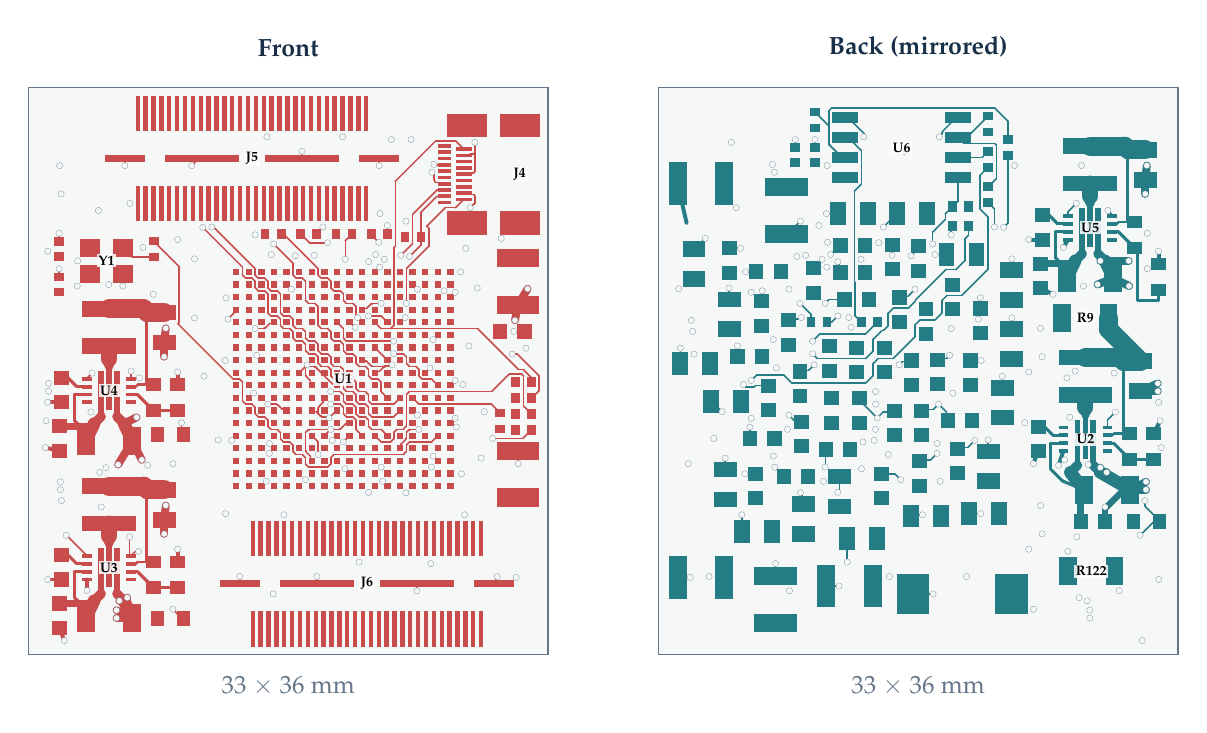
\begin{tikzpicture}[x=0.20cm,y=-0.20cm]
\begin{scope}[shift={(0,0)}]
\fill[boardbg] (0,0) rectangle (33,36);
\draw[muted,line width=.5pt] (0,0) rectangle (33,36);
\node[anchor=south,font=\small\bfseries,text=navy] at (16.5,-1.3) {Front};
\draw[frontcu,line width=0.4000mm,line cap=round] (3.075000,18.985000) -- (2.525000,18.435000);
\draw[frontcu,line width=0.4000mm,line cap=round] (2.525000,18.435000) -- (2.125000,18.435000);
\draw[frontcu,line width=0.4000mm,line cap=round] (3.725000,18.985000) -- (3.075000,18.985000);
\draw[frontcu,line width=0.2000mm,line cap=round] (14.950000,15.300000) -- (14.400000,15.300000);
\draw[frontcu,line width=0.2000mm,line cap=round] (22.075000,18.100000) -- (22.150000,18.025000);
\draw[frontcu,line width=0.2000mm,line cap=round] (17.850000,21.700000) -- (19.200000,21.700000);
\draw[frontcu,line width=0.7000mm,line cap=round] (5.625000,19.235000) -- (5.625000,20.885000);
\draw[frontcu,line width=0.2000mm,line cap=round] (21.200000,17.300000) -- (21.275000,17.300000);
\draw[frontcu,line width=0.2000mm,line cap=round] (28.050000,4.225000) -- (28.275000,4.225000);
\draw[frontcu,line width=0.2000mm,line cap=round] (6.125000,4.500000) -- (6.125000,4.950000);
\draw[frontcu,line width=0.2000mm,line cap=round] (19.775000,21.675000) -- (19.750000,21.700000);
\draw[frontcu,line width=0.2000mm,line cap=round] (18.800000,21.275000) -- (19.100000,20.975000);
\draw[frontcu,line width=0.2000mm,line cap=round] (28.050000,5.425000) -- (28.275000,5.425000);
\draw[frontcu,line width=0.2000mm,line cap=round] (18.400000,20.350000) -- (18.400000,20.700000);
\draw[frontcu,line width=0.2000mm,line cap=round] (25.875000,6.025000) -- (25.825000,5.975000);
\draw[frontcu,line width=0.2000mm,line cap=round] (18.200000,17.725000) -- (18.175000,17.725000);
\draw[frontcu,line width=0.2000mm,line cap=round] (24.000000,21.900000) -- (24.150000,21.750000);
\draw[frontcu,line width=0.2000mm,line cap=round] (17.825000,21.725000) -- (17.850000,21.700000);
\draw[frontcu,line width=0.2000mm,line cap=round] (18.075000,20.500000) -- (18.150000,20.575000);
\draw[frontcu,line width=0.2000mm,line cap=round] (19.575000,20.500000) -- (19.100000,20.975000);
\draw[frontcu,line width=0.2000mm,line cap=round] (28.275000,6.775000) -- (28.325000,6.825000);
\draw[frontcu,line width=0.2000mm,line cap=round] (23.975000,22.275000) -- (24.000000,22.250000);
\draw[frontcu,line width=0.2000mm,line cap=round] (22.800000,9.300000) -- (22.800000,8.750000);
\draw[frontcu,line width=0.2000mm,line cap=round] (18.425000,20.300000) -- (18.425000,20.325000);
\draw[frontcu,line width=0.2000mm,line cap=round] (6.135000,4.500000) -- (6.125000,4.500000);
\draw[frontcu,line width=0.2000mm,line cap=round] (24.675000,31.500000) -- (24.675000,31.950000);
\draw[frontcu,line width=0.2000mm,line cap=round] (28.375000,3.500000) -- (28.350000,3.475000);
\draw[frontcu,line width=0.2000mm,line cap=round] (18.600000,20.875000) -- (18.625000,20.875000);
\draw[frontcu,line width=0.2000mm,line cap=round] (18.200000,17.725000) -- (18.175000,17.725000);
\draw[frontcu,line width=0.2000mm,line cap=round] (18.250000,17.750000) -- (18.225000,17.750000);
\draw[frontcu,line width=0.2000mm,line cap=round] (17.600000,23.050000) -- (17.600000,21.900000);
\draw[frontcu,line width=0.2000mm,line cap=round] (18.450000,20.275000) -- (18.425000,20.300000);
\draw[frontcu,line width=0.2000mm,line cap=round] (11.025000,4.500000) -- (10.950000,4.500000);
\draw[frontcu,line width=0.2000mm,line cap=round] (28.350000,4.075000) -- (28.375000,4.050000);
\draw[frontcu,line width=0.2000mm,line cap=round] (17.625000,18.300000) -- (17.625000,18.275000);
\draw[frontcu,line width=0.2000mm,line cap=round] (17.750000,21.750000) -- (17.775000,21.750000);
\draw[frontcu,line width=0.5000mm,line cap=round] (2.125000,19.985000) -- (1.225000,19.985000);
\draw[frontcu,line width=0.2000mm,line cap=round] (19.450000,18.825000) -- (19.325000,18.825000);
\draw[frontcu,line width=1.2000mm,line cap=round] (5.625000,32.134999) -- (6.075000,32.585000);
\draw[frontcu,line width=0.2000mm,line cap=round] (27.650000,6.700000) -- (27.800000,6.700000);
\draw[frontcu,line width=0.2000mm,line cap=round] (18.625000,20.875000) -- (18.650000,20.900000);
\draw[frontcu,line width=0.2000mm,line cap=round] (22.625000,17.725000) -- (22.650000,17.700000);
\draw[frontcu,line width=0.2000mm,line cap=round] (22.810000,9.300000) -- (22.800000,9.300000);
\draw[frontcu,line width=0.2000mm,line cap=round] (18.575000,20.850000) -- (18.600000,20.875000);
\draw[frontcu,line width=0.2000mm,line cap=round] (19.025000,20.900000) -- (19.100000,20.975000);
\draw[frontcu,line width=0.2000mm,line cap=round] (28.050000,6.775000) -- (28.275000,6.775000);
\draw[frontcu,line width=0.2000mm,line cap=round] (21.850000,17.700000) -- (22.575000,17.700000);
\draw[frontcu,line width=0.2000mm,line cap=round] (29.650000,31.350000) -- (29.650000,31.175000);
\draw[frontcu,line width=0.2000mm,line cap=round] (31.100001,23.075000) -- (31.100000,23.075000);
\draw[frontcu,line width=0.2000mm,line cap=round] (25.825000,5.950000) -- (25.800000,5.925000);
\draw[frontcu,line width=0.2000mm,line cap=round] (18.725000,18.100000) -- (18.650000,18.025000);
\draw[frontcu,line width=0.2000mm,line cap=round] (28.025000,5.450000) -- (28.050000,5.425000);
\draw[frontcu,line width=1.0000mm,line cap=round] (8.625000,27.435000) -- (8.625000,28.335000);
\draw[frontcu,line width=0.2000mm,line cap=round] (19.600000,18.900000) -- (19.525000,18.900000);
\draw[frontcu,line width=0.2000mm,line cap=round] (17.800000,17.700000) -- (17.700000,17.600000);
\draw[frontcu,line width=0.2000mm,line cap=round] (24.175000,21.750000) -- (24.200000,21.725000);
\draw[frontcu,line width=1.0000mm,line cap=round] (31.100000,13.775000) -- (31.700000,12.775000);
\draw[frontcu,line width=0.2000mm,line cap=round] (21.350000,14.025000) -- (21.475000,14.025000);
\draw[frontcu,line width=0.2000mm,line cap=round] (18.450000,20.250000) -- (18.450000,20.275000);
\draw[frontcu,line width=0.2000mm,line cap=round] (23.600000,22.900000) -- (23.600000,22.825000);
\draw[frontcu,line width=0.2000mm,line cap=round] (21.850000,13.700000) -- (22.400000,13.700000);
\draw[frontcu,line width=0.2000mm,line cap=round] (28.375000,6.950000) -- (28.375000,7.325000);
\draw[frontcu,line width=0.2000mm,line cap=round] (28.325000,4.150000) -- (28.350000,4.125000);
\draw[frontcu,line width=0.2000mm,line cap=round] (18.800000,18.100000) -- (18.725000,18.100000);
\draw[frontcu,line width=0.2000mm,line cap=round] (13.425000,31.500000) -- (13.425000,31.050000);
\draw[frontcu,line width=0.2000mm,line cap=round] (19.325000,18.825000) -- (18.250000,17.750000);
\draw[frontcu,line width=0.2000mm,line cap=round] (21.475000,14.025000) -- (21.750000,13.750000);
\draw[frontcu,line width=0.2000mm,line cap=round] (22.000000,11.700000) -- (22.300000,11.400000);
\draw[frontcu,line width=0.2000mm,line cap=round] (27.850000,4.250000) -- (28.025000,4.250000);
\draw[frontcu,line width=0.2000mm,line cap=round] (31.505000,15.480000) -- (31.500000,15.475000);
\draw[frontcu,line width=0.2000mm,line cap=round] (22.575000,17.700000) -- (22.600000,17.675000);
\draw[frontcu,line width=0.2000mm,line cap=round] (18.800000,21.300000) -- (18.800000,21.275000);
\draw[frontcu,line width=0.7000mm,line cap=round] (5.625000,30.485000) -- (5.625000,32.134999);
\draw[frontcu,line width=0.2000mm,line cap=round] (18.800000,22.100000) -- (19.200000,21.700000);
\draw[frontcu,line width=0.2000mm,line cap=round] (14.800000,17.300000) -- (14.500000,17.000000);
\draw[frontcu,line width=1.0000mm,line cap=round] (6.075000,32.585000) -- (5.775000,32.585000);
\draw[frontcu,line width=0.2000mm,line cap=round] (26.800000,21.300000) -- (27.100000,21.000000);
\draw[frontcu,line width=0.2000mm,line cap=round] (28.325000,5.350000) -- (28.350000,5.325000);
\draw[frontcu,line width=0.2000mm,line cap=round] (15.825000,20.150000) -- (15.800000,20.125000);
\draw[frontcu,line width=0.2000mm,line cap=round] (18.000000,20.500000) -- (18.075000,20.500000);
\draw[frontcu,line width=0.2000mm,line cap=round] (18.310000,9.300000) -- (18.300000,9.300000);
\draw[frontcu,line width=1.0000mm,line cap=round] (6.075000,32.585000) -- (6.275000,32.384999);
\draw[frontcu,line width=0.2000mm,line cap=round] (10.875000,4.575000) -- (10.750000,4.575000);
\draw[frontcu,line width=0.2000mm,line cap=round] (20.400000,24.500000) -- (20.100000,24.200000);
\draw[frontcu,line width=0.2000mm,line cap=round] (26.000000,23.700000) -- (25.700000,23.400000);
\draw[frontcu,line width=0.2000mm,line cap=round] (24.225000,21.725000) -- (24.250000,21.700000);
\draw[frontcu,line width=0.2000mm,line cap=round] (28.350000,6.925000) -- (28.375000,6.950000);
\draw[frontcu,line width=0.2000mm,line cap=round] (25.775000,5.525000) -- (25.625000,5.375000);
\draw[frontcu,line width=1.0000mm,line cap=round] (6.600000,33.684999) -- (5.600000,33.684999);
\draw[frontcu,line width=0.2000mm,line cap=round] (17.600000,17.700000) -- (17.700000,17.600000);
\draw[frontcu,line width=0.2000mm,line cap=round] (17.775000,21.750000) -- (17.800000,21.725000);
\draw[frontcu,line width=0.2000mm,line cap=round] (23.025000,17.675000) -- (23.100000,17.600000);
\draw[frontcu,line width=0.2000mm,line cap=round] (25.800000,5.925000) -- (25.800000,5.875000);
\draw[frontcu,line width=0.2000mm,line cap=round] (17.375000,4.500000) -- (17.375000,4.050000);
\draw[frontcu,line width=0.2000mm,line cap=round] (1.960000,12.020001) -- (1.950000,12.025000);
\draw[frontcu,line width=0.2000mm,line cap=round] (19.050000,20.925000) -- (19.100000,20.975000);
\draw[frontcu,line width=0.5000mm,line cap=round] (3.725000,31.235000) -- (3.725000,31.935000);
\draw[frontcu,line width=1.0000mm,line cap=round] (6.600000,33.684999) -- (5.600000,33.184998);
\draw[frontcu,line width=0.2000mm,line cap=round] (16.125000,20.425000) -- (15.850000,20.150000);
\draw[frontcu,line width=0.2000mm,line cap=round] (27.800000,6.700000) -- (27.850000,6.750000);
\draw[frontcu,line width=0.2000mm,line cap=round] (18.150000,20.575000) -- (18.275000,20.575000);
\draw[frontcu,line width=0.2000mm,line cap=round] (23.675000,22.750000) -- (23.675000,22.625000);
\draw[frontcu,line width=0.2000mm,line cap=round] (24.400000,20.500000) -- (24.700000,20.800000);
\draw[frontcu,line width=0.2000mm,line cap=round] (26.800000,13.300000) -- (27.100000,13.000000);
\draw[frontcu,line width=0.2000mm,line cap=round] (18.000000,18.900000) -- (18.000000,18.825000);
\draw[frontcu,line width=0.2000mm,line cap=round] (17.800000,17.700000) -- (17.700000,17.600000);
\draw[frontcu,line width=0.2000mm,line cap=round] (18.575000,20.850000) -- (18.600000,20.875000);
\draw[frontcu,line width=0.2000mm,line cap=round] (22.550000,17.750000) -- (22.575000,17.750000);
\draw[frontcu,line width=0.2000mm,line cap=round] (15.025000,15.250000) -- (15.000000,15.275000);
\draw[frontcu,line width=0.2000mm,line cap=round] (28.325000,5.375000) -- (28.325000,5.350000);
\draw[frontcu,line width=0.2000mm,line cap=round] (19.800000,21.675000) -- (19.775000,21.675000);
\draw[frontcu,line width=0.2000mm,line cap=round] (28.275000,5.425000) -- (28.325000,5.375000);
\draw[frontcu,line width=0.2000mm,line cap=round] (15.050000,15.250000) -- (15.025000,15.250000);
\draw[frontcu,line width=0.2000mm,line cap=round] (17.650000,23.150000) -- (17.650000,23.125000);
\draw[frontcu,line width=0.2000mm,line cap=round] (21.825000,17.675000) -- (21.850000,17.700000);
\draw[frontcu,line width=1.0000mm,line cap=round] (8.625000,27.435000) -- (8.725000,26.535000);
\draw[frontcu,line width=0.2000mm,line cap=round] (22.800000,25.300000) -- (22.500000,25.000000);
\draw[frontcu,line width=0.2000mm,line cap=round] (21.775000,17.650000) -- (21.800000,17.675000);
\draw[frontcu,line width=0.2000mm,line cap=round] (28.375000,5.250000) -- (28.375000,3.500000);
\draw[frontcu,line width=0.2000mm,line cap=round] (29.575000,31.500000) -- (29.575000,31.425000);
\draw[frontcu,line width=0.2000mm,line cap=round] (23.675000,22.625000) -- (23.950000,22.350000);
\draw[frontcu,line width=0.2000mm,line cap=round] (17.925000,23.550000) -- (17.925000,23.425000);
\draw[frontcu,line width=0.2000mm,line cap=round] (20.325000,21.300000) -- (20.250000,21.375000);
\draw[frontcu,line width=0.2000mm,line cap=round] (1.950000,9.775000) -- (1.950000,9.250000);
\draw[frontcu,line width=0.2000mm,line cap=round] (18.225000,17.750000) -- (18.200000,17.725000);
\draw[frontcu,line width=0.2000mm,line cap=round] (28.350000,6.875000) -- (28.350000,6.925000);
\draw[frontcu,line width=0.2000mm,line cap=round] (13.200000,14.175000) -- (12.675000,14.700000);
\draw[frontcu,line width=0.2000mm,line cap=round] (18.300000,9.250000) -- (18.700000,8.850000);
\draw[frontcu,line width=0.2000mm,line cap=round] (26.025000,6.025000) -- (25.875000,6.025000);
\draw[frontcu,line width=0.2000mm,line cap=round] (28.350000,4.125000) -- (28.350000,4.075000);
\draw[frontcu,line width=0.2000mm,line cap=round] (23.600000,14.900000) -- (23.625000,14.900000);
\draw[frontcu,line width=0.2000mm,line cap=round] (17.925000,18.750000) -- (17.925000,18.625000);
\draw[frontcu,line width=0.2000mm,line cap=round] (17.625000,18.275000) -- (17.600000,18.250000);
\draw[frontcu,line width=0.2000mm,line cap=round] (22.275000,18.025000) -- (22.550000,17.750000);
\draw[frontcu,line width=0.2000mm,line cap=round] (18.000000,18.825000) -- (17.925000,18.750000);
\draw[frontcu,line width=0.2000mm,line cap=round] (15.750000,20.100000) -- (15.200000,20.100000);
\draw[frontcu,line width=0.2000mm,line cap=round] (15.775000,20.125000) -- (15.750000,20.100000);
\draw[frontcu,line width=0.2000mm,line cap=round] (17.925000,18.625000) -- (17.650000,18.350000);
\draw[frontcu,line width=0.2000mm,line cap=round] (18.175000,17.725000) -- (18.150000,17.700000);
\draw[frontcu,line width=0.2000mm,line cap=round] (26.050000,6.050000) -- (26.025000,6.025000);
\draw[frontcu,line width=1.0000mm,line cap=round] (6.075000,21.335000) -- (6.875000,20.935000);
\draw[frontcu,line width=0.2000mm,line cap=round] (24.400000,12.500000) -- (24.700000,12.800000);
\draw[frontcu,line width=1.0000mm,line cap=round] (8.625000,16.184999) -- (8.625000,17.085000);
\draw[frontcu,line width=0.2000mm,line cap=round] (26.425000,6.100000) -- (26.275000,6.100000);
\draw[frontcu,line width=0.2000mm,line cap=round] (28.325000,4.175000) -- (28.325000,4.150000);
\draw[frontcu,line width=0.2000mm,line cap=round] (14.800000,25.300000) -- (15.100000,25.000000);
\draw[frontcu,line width=0.2000mm,line cap=round] (21.800000,17.675000) -- (21.825000,17.675000);
\draw[frontcu,line width=0.2000mm,line cap=round] (31.100000,23.075000) -- (31.100000,23.875000);
\draw[frontcu,line width=0.2000mm,line cap=round] (27.650000,4.300000) -- (27.800000,4.300000);
\draw[frontcu,line width=0.2000mm,line cap=round] (18.650000,18.025000) -- (18.525000,18.025000);
\draw[frontcu,line width=0.2000mm,line cap=round] (15.850000,20.150000) -- (15.825000,20.150000);
\draw[frontcu,line width=0.2000mm,line cap=round] (13.435000,31.500000) -- (13.425000,31.500000);
\draw[frontcu,line width=0.2000mm,line cap=round] (19.525000,18.900000) -- (19.450000,18.825000);
\draw[frontcu,line width=0.2000mm,line cap=round] (15.800000,20.125000) -- (15.775000,20.125000);
\draw[frontcu,line width=0.2000mm,line cap=round] (1.960000,9.770001) -- (1.950000,9.775000);
\draw[frontcu,line width=0.5000mm,line cap=round] (1.975000,23.060000) -- (1.075000,22.860000);
\draw[frontcu,line width=0.2000mm,line cap=round] (18.425000,20.325000) -- (18.400000,20.350000);
\draw[frontcu,line width=0.2000mm,line cap=round] (27.800000,5.500000) -- (27.850000,5.450000);
\draw[frontcu,line width=0.2000mm,line cap=round] (18.000000,23.625000) -- (17.925000,23.550000);
\draw[frontcu,line width=0.2000mm,line cap=round] (23.975000,22.300000) -- (23.975000,22.275000);
\draw[frontcu,line width=1.0000mm,line cap=round] (6.600000,22.435000) -- (7.200000,23.635000);
\draw[frontcu,line width=0.2000mm,line cap=round] (27.800000,4.300000) -- (27.850000,4.250000);
\draw[frontcu,line width=0.2000mm,line cap=round] (22.575000,17.750000) -- (22.600000,17.725000);
\draw[frontcu,line width=0.2000mm,line cap=round] (18.300000,9.300000) -- (18.300000,9.250000);
\draw[frontcu,line width=0.2000mm,line cap=round] (17.925000,23.425000) -- (17.650000,23.150000);
\draw[frontcu,line width=0.2000mm,line cap=round] (28.375000,7.325000) -- (28.325000,7.375000);
\draw[frontcu,line width=0.2000mm,line cap=round] (24.250000,21.700000) -- (24.800000,21.700000);
\draw[frontcu,line width=0.2000mm,line cap=round] (19.825000,21.650000) -- (19.800000,21.675000);
\draw[frontcu,line width=0.2000mm,line cap=round] (21.350000,17.375000) -- (21.475000,17.375000);
\draw[frontcu,line width=0.5000mm,line cap=round] (9.475000,18.860000) -- (9.475000,18.060000);
\draw[frontcu,line width=0.2000mm,line cap=round] (23.625000,14.900000) -- (23.925000,14.600000);
\draw[frontcu,line width=0.2000mm,line cap=round] (26.000000,15.700000) -- (25.700000,16.000000);
\draw[frontcu,line width=0.2000mm,line cap=round] (18.725000,20.925000) -- (19.050000,20.925000);
\draw[frontcu,line width=0.2000mm,line cap=round] (27.650000,5.500000) -- (27.800000,5.500000);
\draw[frontcu,line width=0.2000mm,line cap=round] (23.950000,22.350000) -- (23.950000,22.325000);
\draw[frontcu,line width=0.2000mm,line cap=round] (18.325000,31.500000) -- (18.325000,31.050000);
\draw[frontcu,line width=0.2000mm,line cap=round] (28.275000,4.225000) -- (28.325000,4.175000);
\draw[frontcu,line width=0.2000mm,line cap=round] (17.600000,21.900000) -- (17.750000,21.750000);
\draw[frontcu,line width=0.2000mm,line cap=round] (15.325000,14.975000) -- (15.050000,15.250000);
\draw[frontcu,line width=0.2000mm,line cap=round] (17.600000,18.250000) -- (17.600000,17.700000);
\draw[frontcu,line width=0.2000mm,line cap=round] (21.475000,17.375000) -- (21.750000,17.650000);
\draw[frontcu,line width=0.2000mm,line cap=round] (17.650000,18.325000) -- (17.625000,18.300000);
\draw[frontcu,line width=0.5000mm,line cap=round] (1.975000,34.309999) -- (2.275000,35.109999);
\draw[frontcu,line width=0.2000mm,line cap=round] (17.200000,18.100000) -- (17.700000,17.600000);
\draw[frontcu,line width=0.2000mm,line cap=round] (22.000000,16.500000) -- (23.100000,17.600000);
\draw[frontcu,line width=0.2000mm,line cap=round] (18.725000,19.975000) -- (18.450000,20.250000);
\draw[frontcu,line width=0.2000mm,line cap=round] (25.200000,18.100000) -- (25.500000,17.800000);
\draw[frontcu,line width=0.2000mm,line cap=round] (19.850000,21.650000) -- (19.825000,21.650000);
\draw[frontcu,line width=1.6000mm,line cap=round] (6.075000,32.585000) -- (6.600000,33.684999);
\draw[frontcu,line width=0.2000mm,line cap=round] (21.200000,14.100000) -- (21.275000,14.100000);
\draw[frontcu,line width=0.2000mm,line cap=round] (28.325000,6.850000) -- (28.350000,6.875000);
\draw[frontcu,line width=0.2000mm,line cap=round] (1.950000,12.025000) -- (1.950000,11.500000);
\draw[frontcu,line width=0.2000mm,line cap=round] (17.625000,23.075000) -- (17.600000,23.050000);
\draw[frontcu,line width=0.2000mm,line cap=round] (25.775000,5.850000) -- (25.775000,5.525000);
\draw[frontcu,line width=0.2000mm,line cap=round] (21.275000,14.100000) -- (21.350000,14.025000);
\draw[frontcu,line width=1.0000mm,line cap=round] (31.100000,13.775000) -- (30.900000,14.775000);
\draw[frontcu,line width=0.2000mm,line cap=round] (25.800000,5.875000) -- (25.775000,5.850000);
\draw[frontcu,line width=1.0000mm,line cap=round] (6.600000,22.435000) -- (5.700000,23.935000);
\draw[frontcu,line width=0.2000mm,line cap=round] (28.375000,3.500000) -- (28.350000,3.475000);
\draw[frontcu,line width=0.2000mm,line cap=round] (19.750000,21.700000) -- (19.200000,21.700000);
\draw[frontcu,line width=0.2000mm,line cap=round] (18.225000,17.750000) -- (18.200000,17.725000);
\draw[frontcu,line width=0.2000mm,line cap=round] (21.775000,13.750000) -- (21.800000,13.725000);
\draw[frontcu,line width=0.2000mm,line cap=round] (13.200000,22.100000) -- (12.900000,22.400000);
\draw[frontcu,line width=0.2000mm,line cap=round] (17.625000,23.100000) -- (17.625000,23.075000);
\draw[frontcu,line width=0.2000mm,line cap=round] (28.350000,5.325000) -- (28.350000,5.275000);
\draw[frontcu,line width=0.2000mm,line cap=round] (22.600000,17.725000) -- (22.625000,17.725000);
\draw[frontcu,line width=0.2000mm,line cap=round] (18.600000,20.875000) -- (18.625000,20.875000);
\draw[frontcu,line width=0.2000mm,line cap=round] (29.565000,31.500000) -- (29.575000,31.500000);
\draw[frontcu,line width=0.2000mm,line cap=round] (18.725000,19.850000) -- (18.725000,19.975000);
\draw[frontcu,line width=0.2000mm,line cap=round] (21.825000,13.725000) -- (21.850000,13.700000);
\draw[frontcu,line width=0.2000mm,line cap=round] (28.325000,6.825000) -- (28.325000,6.850000);
\draw[frontcu,line width=0.2000mm,line cap=round] (23.600000,22.825000) -- (23.675000,22.750000);
\draw[frontcu,line width=0.2000mm,line cap=round] (22.275000,4.500000) -- (22.275000,4.950000);
\draw[frontcu,line width=0.2000mm,line cap=round] (26.225000,6.050000) -- (26.050000,6.050000);
\draw[frontcu,line width=0.2000mm,line cap=round] (16.250000,20.425000) -- (16.125000,20.425000);
\draw[frontcu,line width=0.2000mm,line cap=round] (20.400000,21.300000) -- (20.325000,21.300000);
\draw[frontcu,line width=0.2000mm,line cap=round] (21.800000,13.725000) -- (21.825000,13.725000);
\draw[frontcu,line width=0.2000mm,line cap=round] (22.150000,18.025000) -- (22.275000,18.025000);
\draw[frontcu,line width=0.2000mm,line cap=round] (24.200000,21.725000) -- (24.225000,21.725000);
\draw[frontcu,line width=0.2000mm,line cap=round] (27.850000,5.450000) -- (28.025000,5.450000);
\draw[frontcu,line width=0.2000mm,line cap=round] (15.600000,22.900000) -- (15.300000,22.600000);
\draw[frontcu,line width=0.2000mm,line cap=round] (25.775000,4.900000) -- (25.750000,4.875000);
\draw[frontcu,line width=0.2000mm,line cap=round] (14.000000,19.700000) -- (14.300000,19.400000);
\draw[frontcu,line width=0.2000mm,line cap=round] (18.550000,20.850000) -- (18.575000,20.850000);
\draw[frontcu,line width=0.2000mm,line cap=round] (28.025000,4.250000) -- (28.050000,4.225000);
\draw[frontcu,line width=0.2000mm,line cap=round] (18.625000,20.875000) -- (18.650000,20.900000);
\draw[frontcu,line width=0.2000mm,line cap=round] (18.700000,20.900000) -- (18.725000,20.925000);
\draw[frontcu,line width=0.2000mm,line cap=round] (18.550000,20.850000) -- (18.575000,20.850000);
\draw[frontcu,line width=0.2000mm,line cap=round] (16.399999,20.500000) -- (16.325000,20.500000);
\draw[frontcu,line width=0.2000mm,line cap=round] (26.275000,6.100000) -- (26.225000,6.050000);
\draw[frontcu,line width=1.6000mm,line cap=round] (6.075000,21.335000) -- (6.600000,22.435000);
\draw[frontcu,line width=0.2000mm,line cap=round] (21.275000,17.300000) -- (21.350000,17.375000);
\draw[frontcu,line width=0.2000mm,line cap=round] (22.265000,4.500000) -- (22.275000,4.500000);
\draw[frontcu,line width=0.2000mm,line cap=round] (17.650000,23.125000) -- (17.625000,23.100000);
\draw[frontcu,line width=0.2000mm,line cap=round] (21.750000,13.750000) -- (21.775000,13.750000);
\draw[frontcu,line width=0.2000mm,line cap=round] (16.399999,12.500000) -- (16.700000,12.800000);
\draw[frontcu,line width=0.2000mm,line cap=round] (15.450000,14.975000) -- (15.325000,14.975000);
\draw[frontcu,line width=0.5000mm,line cap=round] (9.475000,30.110000) -- (9.475000,29.310000);
\draw[frontcu,line width=0.2000mm,line cap=round] (13.200000,14.100000) -- (13.200000,14.175000);
\draw[frontcu,line width=0.2000mm,line cap=round] (27.850000,6.750000) -- (28.025000,6.750000);
\draw[frontcu,line width=0.2000mm,line cap=round] (29.575000,31.425000) -- (29.650000,31.350000);
\draw[frontcu,line width=0.2000mm,line cap=round] (23.950000,22.325000) -- (23.975000,22.300000);
\draw[frontcu,line width=0.2000mm,line cap=round] (23.000000,17.700000) -- (23.100000,17.600000);
\draw[frontcu,line width=0.2000mm,line cap=round] (18.800000,19.775000) -- (18.725000,19.850000);
\draw[frontcu,line width=0.2000mm,line cap=round] (18.800000,19.700000) -- (18.800000,19.775000);
\draw[frontcu,line width=0.2000mm,line cap=round] (15.525000,14.900000) -- (15.450000,14.975000);
\draw[frontcu,line width=0.2000mm,line cap=round] (28.350000,5.275000) -- (28.375000,5.250000);
\draw[frontcu,line width=1.2000mm,line cap=round] (5.625000,20.885000) -- (6.075000,21.335000);
\draw[frontcu,line width=0.2000mm,line cap=round] (18.650000,20.900000) -- (18.700000,20.900000);
\draw[frontcu,line width=0.2000mm,line cap=round] (28.025000,6.750000) -- (28.050000,6.775000);
\draw[frontcu,line width=0.2000mm,line cap=round] (18.250000,17.750000) -- (18.225000,17.750000);
\draw[frontcu,line width=0.2000mm,line cap=round] (24.000000,22.250000) -- (24.000000,21.900000);
\draw[frontcu,line width=0.2000mm,line cap=round] (15.000000,15.275000) -- (14.975000,15.275000);
\draw[frontcu,line width=0.2000mm,line cap=round] (18.525000,18.025000) -- (18.250000,17.750000);
\draw[frontcu,line width=0.2000mm,line cap=round] (31.500000,15.475000) -- (30.825000,15.475000);
\draw[frontcu,line width=0.2000mm,line cap=round] (17.650000,18.350000) -- (17.650000,18.325000);
\draw[frontcu,line width=0.2000mm,line cap=round] (14.975000,15.275000) -- (14.950000,15.300000);
\draw[frontcu,line width=0.2000mm,line cap=round] (20.125000,21.375000) -- (19.850000,21.650000);
\draw[frontcu,line width=0.2000mm,line cap=round] (16.325000,20.500000) -- (16.250000,20.425000);
\draw[frontcu,line width=0.2000mm,line cap=round] (21.750000,17.650000) -- (21.775000,17.650000);
\draw[frontcu,line width=0.2000mm,line cap=round] (28.325000,7.375000) -- (28.300000,7.375000);
\draw[frontcu,line width=0.2000mm,line cap=round] (24.150000,21.750000) -- (24.175000,21.750000);
\draw[frontcu,line width=0.2000mm,line cap=round] (18.650000,20.900000) -- (19.025000,20.900000);
\draw[frontcu,line width=0.2000mm,line cap=round] (15.600000,14.900000) -- (15.525000,14.900000);
\draw[frontcu,line width=0.2000mm,line cap=round] (17.800000,21.725000) -- (17.825000,21.725000);
\draw[frontcu,line width=0.2000mm,line cap=round] (18.275000,20.575000) -- (18.550000,20.850000);
\draw[frontcu,line width=0.2000mm,line cap=round] (18.175000,17.725000) -- (18.150000,17.700000);
\draw[frontcu,line width=0.2000mm,line cap=round] (28.375000,4.050000) -- (28.375000,3.500000);
\draw[frontcu,line width=0.2000mm,line cap=round] (29.650000,31.175000) -- (29.775000,31.050000);
\draw[frontcu,line width=0.2000mm,line cap=round] (6.010000,11.825001) -- (6.000000,11.825000);
\draw[frontcu,line width=0.2000mm,line cap=round] (6.000000,11.825000) -- (6.000000,12.600000);
\draw[frontcu,line width=0.2000mm,line cap=round] (19.600000,20.500000) -- (19.575000,20.500000);
\draw[frontcu,line width=0.2000mm,line cap=round] (10.750000,4.575000) -- (10.375000,4.950000);
\draw[frontcu,line width=0.2000mm,line cap=round] (26.425000,4.900000) -- (25.775000,4.900000);
\draw[frontcu,line width=0.2000mm,line cap=round] (18.150000,17.700000) -- (17.800000,17.700000);
\draw[frontcu,line width=0.2000mm,line cap=round] (20.250000,21.375000) -- (20.125000,21.375000);
\draw[frontcu,line width=0.2000mm,line cap=round] (22.000000,18.100000) -- (22.075000,18.100000);
\draw[frontcu,line width=1.0000mm,line cap=round] (8.625000,16.184999) -- (8.725000,15.285000);
\draw[frontcu,line width=0.5000mm,line cap=round] (2.125000,31.235000) -- (1.225000,31.235000);
\draw[frontcu,line width=0.2000mm,line cap=round] (28.300000,7.375000) -- (28.050000,7.625000);
\draw[frontcu,line width=0.2000mm,line cap=round] (10.950000,4.500000) -- (10.875000,4.575000);
\draw[frontcu,line width=0.2000mm,line cap=round] (18.400000,20.700000) -- (18.550000,20.850000);
\draw[frontcu,line width=0.2000mm,line cap=round] (22.600000,17.675000) -- (23.025000,17.675000);
\draw[frontcu,line width=0.2000mm,line cap=round] (18.000000,23.700000) -- (18.000000,23.625000);
\draw[frontcu,line width=0.2000mm,line cap=round] (25.825000,5.975000) -- (25.825000,5.950000);
\draw[frontcu,line width=0.2000mm,line cap=round] (18.150000,17.700000) -- (17.800000,17.700000);
\draw[frontcu,line width=0.2000mm,line cap=round] (18.000000,17.300000) -- (17.700000,17.600000);
\draw[frontcu,line width=0.2000mm,line cap=round] (22.650000,17.700000) -- (23.000000,17.700000);
\draw[frontcu,line width=0.4000mm,line cap=round] (2.925000,30.735000) -- (2.925000,32.384999);
\draw[frontcu,line width=1.2000mm,line cap=round] (4.625000,32.134999) -- (4.175000,32.585000);
\draw[frontcu,line width=0.8000mm,line cap=round] (1.975000,21.510000) -- (3.800000,21.510000);
\draw[frontcu,line width=1.6000mm,line cap=round] (4.175000,21.335000) -- (3.650000,22.435000);
\draw[frontcu,line width=1.6000mm,line cap=round] (4.175000,32.585000) -- (3.650000,33.684999);
\draw[frontcu,line width=0.8000mm,line cap=round] (1.975000,32.759999) -- (3.800000,32.759999);
\draw[frontcu,line width=0.7000mm,line cap=round] (4.625000,30.485000) -- (4.625000,32.134999);
\draw[frontcu,line width=0.4000mm,line cap=round] (2.925000,21.135000) -- (3.675000,21.885000);
\draw[frontcu,line width=0.4000mm,line cap=round] (2.925000,19.485000) -- (2.925000,21.135000);
\draw[frontcu,line width=1.2000mm,line cap=round] (4.625000,20.885000) -- (4.175000,21.335000);
\draw[frontcu,line width=0.4000mm,line cap=round] (3.675000,21.885000) -- (3.650000,22.435000);
\draw[frontcu,line width=0.4000mm,line cap=round] (3.725000,30.735000) -- (2.925000,30.735000);
\draw[frontcu,line width=0.8000mm,line cap=round] (3.800000,32.759999) -- (3.650000,33.684999);
\draw[frontcu,line width=0.8000mm,line cap=round] (3.800000,21.510000) -- (3.650000,22.435000);
\draw[frontcu,line width=0.4000mm,line cap=round] (2.925000,32.384999) -- (3.675000,33.134999);
\draw[frontcu,line width=0.7000mm,line cap=round] (4.625000,19.235000) -- (4.625000,20.885000);
\draw[frontcu,line width=0.4000mm,line cap=round] (3.725000,19.485000) -- (2.925000,19.485000);
\draw[frontcu,line width=0.4000mm,line cap=round] (3.675000,33.134999) -- (3.650000,33.684999);
\draw[frontcu,line width=0.2000mm,line cap=round] (18.400000,23.300000) -- (18.400000,22.500000);
\draw[frontcu,line width=0.2000mm,line cap=round] (20.560000,9.300000) -- (20.550000,9.300000);
\draw[frontcu,line width=0.2000mm,line cap=round] (20.550000,9.300000) -- (20.125000,9.725000);
\draw[frontcu,line width=0.2000mm,line cap=round] (20.125000,9.725000) -- (20.125000,10.900000);
\draw[frontcu,line width=0.2000mm,line cap=round] (18.400000,22.500000) -- (18.000000,22.100000);
\draw[frontcu,line width=0.2000mm,line cap=round] (29.400000,20.100000) -- (25.050000,20.100000);
\draw[frontcu,line width=0.2000mm,line cap=round] (24.800000,20.100000) -- (24.400000,19.700000);
\draw[frontcu,line width=0.2000mm,line cap=round] (29.970001,20.670000) -- (29.975000,20.675000);
\draw[frontcu,line width=0.2000mm,line cap=round] (25.050000,20.100000) -- (24.800000,20.100000);
\draw[frontcu,line width=0.2000mm,line cap=round] (29.975000,20.675000) -- (29.400000,20.100000);
\draw[frontcu,line width=0.2000mm,line cap=round] (24.950000,9.475000) -- (24.950000,9.975000);
\draw[frontcu,line width=0.2000mm,line cap=round] (24.950000,9.975000) -- (24.200000,10.725000);
\draw[frontcu,line width=0.2000mm,line cap=round] (24.950000,9.475000) -- (24.950000,7.900000);
\draw[frontcu,line width=0.2000mm,line cap=round] (25.950000,6.900000) -- (26.425000,6.900000);
\draw[frontcu,line width=0.2000mm,line cap=round] (24.940001,9.469999) -- (24.950000,9.475000);
\draw[frontcu,line width=0.2000mm,line cap=round] (20.425000,14.900000) -- (20.400000,14.900000);
\draw[frontcu,line width=0.2000mm,line cap=round] (20.750000,15.225000) -- (20.425000,14.900000);
\draw[frontcu,line width=0.2000mm,line cap=round] (25.825000,7.025000) -- (25.950000,6.900000);
\draw[frontcu,line width=0.2000mm,line cap=round] (24.950000,7.900000) -- (25.825000,7.025000);
\draw[frontcu,line width=2.0000mm,line cap=round] (5.125000,17.235000) -- (5.125000,16.420000);
\draw[frontcu,line width=0.7000mm,line cap=round] (5.125000,19.235000) -- (5.125000,17.635000);
\draw[frontcu,line width=1.2000mm,line cap=round] (5.125000,17.635000) -- (5.125000,17.235000);
\draw[frontcu,line width=0.3000mm,line cap=round] (6.525000,18.985000) -- (6.825000,18.985000);
\draw[frontcu,line width=0.4000mm,line cap=round] (8.625000,14.285000) -- (7.525000,14.285000);
\draw[frontcu,line width=0.4000mm,line cap=round] (7.525000,14.285000) -- (7.525000,18.860000);
\draw[frontcu,line width=2.4000mm,line cap=round] (7.560000,14.285000) -- (8.625000,14.285000);
\draw[frontcu,line width=0.4000mm,line cap=round] (7.525000,18.860000) -- (7.925000,18.860000);
\draw[frontcu,line width=2.4000mm,line cap=round] (5.125000,14.050000) -- (7.325000,14.050000);
\draw[frontcu,line width=0.3000mm,line cap=round] (6.950000,18.860000) -- (7.925000,18.860000);
\draw[frontcu,line width=0.3000mm,line cap=round] (6.825000,18.985000) -- (6.950000,18.860000);
\draw[frontcu,line width=2.4000mm,line cap=round] (7.325000,14.050000) -- (7.560000,14.285000);
\draw[frontcu,line width=0.2000mm,line cap=round] (31.950000,18.725000) -- (31.940000,18.720000);
\draw[frontcu,line width=0.2000mm,line cap=round] (23.200000,15.100000) -- (23.050000,15.250000);
\draw[frontcu,line width=0.2000mm,line cap=round] (23.300000,5.950000) -- (23.300000,10.075000);
\draw[frontcu,line width=0.2000mm,line cap=round] (28.525000,15.300000) -- (31.125000,17.900000);
\draw[frontcu,line width=0.2000mm,line cap=round] (22.400000,15.300000) -- (22.000000,14.900000);
\draw[frontcu,line width=0.2000mm,line cap=round] (24.800000,4.450000) -- (23.300000,5.950000);
\draw[frontcu,line width=0.2000mm,line cap=round] (23.200000,10.175000) -- (23.200000,15.050000);
\draw[frontcu,line width=0.2000mm,line cap=round] (26.950000,15.300000) -- (28.525000,15.300000);
\draw[frontcu,line width=0.2000mm,line cap=round] (23.300000,10.075000) -- (23.200000,10.175000);
\draw[frontcu,line width=0.2000mm,line cap=round] (27.125000,3.375000) -- (25.900000,3.375000);
\draw[frontcu,line width=0.2000mm,line cap=round] (23.200000,15.050000) -- (23.200000,15.100000);
\draw[frontcu,line width=0.2000mm,line cap=round] (23.000000,15.300000) -- (22.650000,15.300000);
\draw[frontcu,line width=0.2000mm,line cap=round] (25.875000,3.375000) -- (24.800000,4.450000);
\draw[frontcu,line width=0.2000mm,line cap=round] (31.850000,18.325000) -- (31.950000,18.425000);
\draw[frontcu,line width=0.2000mm,line cap=round] (31.125000,17.900000) -- (31.425000,17.900000);
\draw[frontcu,line width=0.2000mm,line cap=round] (23.050000,15.250000) -- (23.000000,15.300000);
\draw[frontcu,line width=0.2000mm,line cap=round] (31.425000,17.900000) -- (31.850000,18.325000);
\draw[frontcu,line width=0.2000mm,line cap=round] (31.950000,18.425000) -- (31.950000,18.725000);
\draw[frontcu,line width=0.2000mm,line cap=round] (25.900000,3.375000) -- (25.875000,3.375000);
\draw[frontcu,line width=0.2000mm,line cap=round] (27.650000,3.900000) -- (27.125000,3.375000);
\draw[frontcu,line width=0.2000mm,line cap=round] (22.650000,15.300000) -- (22.400000,15.300000);
\draw[frontcu,line width=0.2000mm,line cap=round] (22.400000,15.300000) -- (26.950000,15.300000);
\draw[frontcu,line width=0.2000mm,line cap=round] (20.000000,13.500000) -- (20.000000,13.100000);
\draw[frontcu,line width=0.2000mm,line cap=round] (16.200000,9.300000) -- (16.050000,9.300000);
\draw[frontcu,line width=0.2000mm,line cap=round] (19.400000,12.900000) -- (19.200000,12.700000);
\draw[frontcu,line width=0.2000mm,line cap=round] (18.400000,11.500000) -- (16.250000,9.350000);
\draw[frontcu,line width=0.2000mm,line cap=round] (20.200000,13.700000) -- (20.000000,13.500000);
\draw[frontcu,line width=0.2000mm,line cap=round] (16.250000,9.350000) -- (16.200000,9.300000);
\draw[frontcu,line width=0.2000mm,line cap=round] (24.400000,9.900000) -- (23.650000,10.650000);
\draw[frontcu,line width=0.2000mm,line cap=round] (26.425000,6.500000) -- (25.950000,6.500000);
\draw[frontcu,line width=0.2000mm,line cap=round] (24.400000,9.875000) -- (24.400000,9.900000);
\draw[frontcu,line width=0.2000mm,line cap=round] (20.800000,14.500000) -- (20.800000,13.950000);
\draw[frontcu,line width=0.2000mm,line cap=round] (20.000000,13.100000) -- (19.800000,12.900000);
\draw[frontcu,line width=0.2000mm,line cap=round] (19.000000,12.100000) -- (18.600000,12.100000);
\draw[frontcu,line width=0.2000mm,line cap=round] (21.200000,14.900000) -- (20.800000,14.500000);
\draw[frontcu,line width=0.2000mm,line cap=round] (20.600000,13.700000) -- (20.200000,13.700000);
\draw[frontcu,line width=0.2000mm,line cap=round] (24.400000,8.050000) -- (24.400000,9.875000);
\draw[frontcu,line width=0.2000mm,line cap=round] (20.800000,13.950000) -- (20.800000,13.900000);
\draw[frontcu,line width=0.2000mm,line cap=round] (19.800000,12.900000) -- (19.400000,12.900000);
\draw[frontcu,line width=0.2000mm,line cap=round] (16.050000,9.300000) -- (16.059999,9.300000);
\draw[frontcu,line width=0.2000mm,line cap=round] (18.400000,11.900000) -- (18.400000,11.500000);
\draw[frontcu,line width=0.2000mm,line cap=round] (20.800000,13.900000) -- (20.600000,13.700000);
\draw[frontcu,line width=0.2000mm,line cap=round] (19.200000,12.300000) -- (19.000000,12.100000);
\draw[frontcu,line width=0.2000mm,line cap=round] (19.200000,12.700000) -- (19.200000,12.300000);
\draw[frontcu,line width=0.2000mm,line cap=round] (20.900000,14.600000) -- (21.200000,14.900000);
\draw[frontcu,line width=0.2000mm,line cap=round] (25.950000,6.500000) -- (25.775000,6.675000);
\draw[frontcu,line width=0.2000mm,line cap=round] (25.775000,6.675000) -- (24.400000,8.050000);
\draw[frontcu,line width=0.2000mm,line cap=round] (18.600000,12.100000) -- (18.400000,11.900000);
\draw[frontcu,line width=0.2000mm,line cap=round] (25.425000,8.925000) -- (25.425000,9.875000);
\draw[frontcu,line width=0.2000mm,line cap=round] (27.650000,7.100000) -- (27.125000,7.625000);
\draw[frontcu,line width=0.2000mm,line cap=round] (25.300000,8.800000) -- (25.425000,8.925000);
\draw[frontcu,line width=0.2000mm,line cap=round] (26.475000,7.625000) -- (25.300000,8.800000);
\draw[frontcu,line width=0.2000mm,line cap=round] (24.050000,11.450000) -- (24.000000,11.500000);
\draw[frontcu,line width=0.2000mm,line cap=round] (25.425000,10.075000) -- (24.050000,11.450000);
\draw[frontcu,line width=0.2000mm,line cap=round] (26.525000,7.625000) -- (26.475000,7.625000);
\draw[frontcu,line width=0.2000mm,line cap=round] (24.000000,11.500000) -- (24.000000,13.700000);
\draw[frontcu,line width=0.2000mm,line cap=round] (27.125000,7.625000) -- (26.525000,7.625000);
\draw[frontcu,line width=0.2000mm,line cap=round] (25.425000,9.875000) -- (25.425000,10.075000);
\draw[frontcu,line width=0.2000mm,line cap=round] (20.000000,15.900000) -- (20.200000,16.100000);
\draw[frontcu,line width=0.2000mm,line cap=round] (20.000000,15.300000) -- (20.000000,15.900000);
\draw[frontcu,line width=0.2000mm,line cap=round] (20.200000,16.100000) -- (23.200000,16.100000);
\draw[frontcu,line width=0.2000mm,line cap=round] (19.600000,14.900000) -- (20.000000,15.300000);
\draw[frontcu,line width=0.2000mm,line cap=round] (22.800000,14.900000) -- (22.400000,14.500000);
\draw[frontcu,line width=0.2000mm,line cap=round] (22.400000,14.500000) -- (21.600000,14.500000);
\draw[frontcu,line width=0.2000mm,line cap=round] (23.800000,16.900000) -- (23.200000,16.900000);
\draw[frontcu,line width=0.2000mm,line cap=round] (26.000000,18.900000) -- (25.600000,18.500000);
\draw[frontcu,line width=0.2000mm,line cap=round] (25.000000,18.500000) -- (24.800000,18.300000);
\draw[frontcu,line width=0.2000mm,line cap=round] (24.000000,17.500000) -- (24.000000,17.100000);
\draw[frontcu,line width=0.2000mm,line cap=round] (24.800000,18.300000) -- (24.800000,17.900000);
\draw[frontcu,line width=0.2000mm,line cap=round] (24.000000,17.100000) -- (23.800000,16.900000);
\draw[frontcu,line width=0.2000mm,line cap=round] (24.800000,17.900000) -- (24.600000,17.700000);
\draw[frontcu,line width=0.2000mm,line cap=round] (24.600000,17.700000) -- (24.200000,17.700000);
\draw[frontcu,line width=0.2000mm,line cap=round] (25.600000,18.500000) -- (25.050000,18.500000);
\draw[frontcu,line width=0.2000mm,line cap=round] (24.200000,17.700000) -- (24.000000,17.500000);
\draw[frontcu,line width=0.2000mm,line cap=round] (25.050000,18.500000) -- (25.000000,18.500000);
\draw[frontcu,line width=0.2000mm,line cap=round] (26.800000,18.900000) -- (27.100000,18.600000);
\draw[frontcu,line width=0.2000mm,line cap=round] (21.600000,18.300000) -- (21.600000,17.900000);
\draw[frontcu,line width=0.2000mm,line cap=round] (21.400000,17.700000) -- (21.000000,17.700000);
\draw[frontcu,line width=0.2000mm,line cap=round] (21.600000,17.900000) -- (21.400000,17.700000);
\draw[frontcu,line width=0.2000mm,line cap=round] (22.400000,19.300000) -- (22.400000,18.750000);
\draw[frontcu,line width=0.2000mm,line cap=round] (19.200000,15.900000) -- (19.200000,15.500000);
\draw[frontcu,line width=0.2000mm,line cap=round] (20.000000,16.300000) -- (19.800000,16.100000);
\draw[frontcu,line width=0.2000mm,line cap=round] (19.200000,15.500000) -- (19.000000,15.300000);
\draw[frontcu,line width=0.2000mm,line cap=round] (21.000000,17.700000) -- (20.800000,17.500000);
\draw[frontcu,line width=0.2000mm,line cap=round] (18.600000,15.300000) -- (18.400000,15.100000);
\draw[frontcu,line width=0.2000mm,line cap=round] (20.200000,16.900000) -- (20.000000,16.700000);
\draw[frontcu,line width=0.2000mm,line cap=round] (17.600000,12.300000) -- (17.400000,12.100000);
\draw[frontcu,line width=0.2000mm,line cap=round] (17.400000,12.100000) -- (17.000000,12.100000);
\draw[frontcu,line width=0.2000mm,line cap=round] (19.400000,16.100000) -- (19.200000,15.900000);
\draw[frontcu,line width=0.2000mm,line cap=round] (17.000000,12.100000) -- (16.800000,11.900000);
\draw[frontcu,line width=0.2000mm,line cap=round] (17.800000,13.700000) -- (17.600000,13.500000);
\draw[frontcu,line width=0.2000mm,line cap=round] (18.200000,13.700000) -- (17.800000,13.700000);
\draw[frontcu,line width=0.2000mm,line cap=round] (22.400000,18.750000) -- (22.400000,18.700000);
\draw[frontcu,line width=0.2000mm,line cap=round] (16.800000,11.900000) -- (16.800000,11.150000);
\draw[frontcu,line width=0.2000mm,line cap=round] (21.800000,18.500000) -- (21.600000,18.300000);
\draw[frontcu,line width=0.2000mm,line cap=round] (19.000000,15.300000) -- (18.600000,15.300000);
\draw[frontcu,line width=0.2000mm,line cap=round] (22.200000,18.500000) -- (21.800000,18.500000);
\draw[frontcu,line width=0.2000mm,line cap=round] (17.600000,13.500000) -- (17.600000,12.300000);
\draw[frontcu,line width=0.2000mm,line cap=round] (18.400000,13.900000) -- (18.200000,13.700000);
\draw[frontcu,line width=0.2000mm,line cap=round] (20.600000,16.900000) -- (20.200000,16.900000);
\draw[frontcu,line width=0.2000mm,line cap=round] (20.800000,17.500000) -- (20.800000,17.100000);
\draw[frontcu,line width=0.2000mm,line cap=round] (18.400000,15.100000) -- (18.400000,13.900000);
\draw[frontcu,line width=0.2000mm,line cap=round] (20.000000,16.700000) -- (20.000000,16.300000);
\draw[frontcu,line width=0.2000mm,line cap=round] (22.800000,19.700000) -- (22.400000,19.300000);
\draw[frontcu,line width=0.2000mm,line cap=round] (19.800000,16.100000) -- (19.400000,16.100000);
\draw[frontcu,line width=0.2000mm,line cap=round] (16.800000,11.150000) -- (15.575000,9.925000);
\draw[frontcu,line width=0.2000mm,line cap=round] (22.400000,18.700000) -- (22.200000,18.500000);
\draw[frontcu,line width=0.2000mm,line cap=round] (20.800000,17.100000) -- (20.600000,16.900000);
\draw[frontcu,line width=0.2000mm,line cap=round] (15.200000,12.300000) -- (15.000000,12.100000);
\draw[frontcu,line width=0.2000mm,line cap=round] (14.600000,12.100000) -- (14.400000,11.900000);
\draw[frontcu,line width=0.2000mm,line cap=round] (17.600000,15.900000) -- (17.600000,15.500000);
\draw[frontcu,line width=0.2000mm,line cap=round] (16.800000,15.100000) -- (16.800000,14.700000);
\draw[frontcu,line width=0.2000mm,line cap=round] (14.400000,11.500000) -- (11.750000,8.850000);
\draw[frontcu,line width=0.2000mm,line cap=round] (20.000000,17.900000) -- (19.800000,17.700000);
\draw[frontcu,line width=0.2000mm,line cap=round] (21.000000,19.300000) -- (20.800000,19.100000);
\draw[frontcu,line width=0.2000mm,line cap=round] (15.800000,12.900000) -- (15.400000,12.900000);
\draw[frontcu,line width=0.2000mm,line cap=round] (21.600000,19.900000) -- (21.600000,19.500000);
\draw[frontcu,line width=0.2000mm,line cap=round] (16.800000,14.700000) -- (16.600000,14.500000);
\draw[frontcu,line width=0.2000mm,line cap=round] (21.850000,20.100000) -- (21.800000,20.100000);
\draw[frontcu,line width=0.2000mm,line cap=round] (23.200000,20.100000) -- (21.850000,20.100000);
\draw[frontcu,line width=0.2000mm,line cap=round] (21.800000,20.100000) -- (21.600000,19.900000);
\draw[frontcu,line width=0.2000mm,line cap=round] (19.400000,17.700000) -- (19.200000,17.500000);
\draw[frontcu,line width=0.2000mm,line cap=round] (16.200000,14.500000) -- (16.000000,14.300000);
\draw[frontcu,line width=0.2000mm,line cap=round] (19.800000,17.700000) -- (19.400000,17.700000);
\draw[frontcu,line width=0.2000mm,line cap=round] (15.200000,12.700000) -- (15.200000,12.300000);
\draw[frontcu,line width=0.2000mm,line cap=round] (17.600000,15.500000) -- (17.400000,15.300000);
\draw[frontcu,line width=0.2000mm,line cap=round] (18.400000,16.700000) -- (18.400000,16.300000);
\draw[frontcu,line width=0.2000mm,line cap=round] (15.000000,12.100000) -- (14.600000,12.100000);
\draw[frontcu,line width=0.2000mm,line cap=round] (18.400000,16.300000) -- (18.200000,16.100000);
\draw[frontcu,line width=0.2000mm,line cap=round] (20.200000,18.500000) -- (20.000000,18.300000);
\draw[frontcu,line width=0.2000mm,line cap=round] (17.800000,16.100000) -- (17.600000,15.900000);
\draw[frontcu,line width=0.2000mm,line cap=round] (19.000000,16.900000) -- (18.600000,16.900000);
\draw[frontcu,line width=0.2000mm,line cap=round] (19.200000,17.500000) -- (19.200000,17.100000);
\draw[frontcu,line width=0.2000mm,line cap=round] (14.400000,11.900000) -- (14.400000,11.500000);
\draw[frontcu,line width=0.2000mm,line cap=round] (17.000000,15.300000) -- (16.800000,15.100000);
\draw[frontcu,line width=0.2000mm,line cap=round] (19.200000,17.100000) -- (19.000000,16.900000);
\draw[frontcu,line width=0.2000mm,line cap=round] (18.200000,16.100000) -- (17.800000,16.100000);
\draw[frontcu,line width=0.2000mm,line cap=round] (20.600000,18.500000) -- (20.200000,18.500000);
\draw[frontcu,line width=0.2000mm,line cap=round] (20.800000,19.100000) -- (20.800000,18.700000);
\draw[frontcu,line width=0.2000mm,line cap=round] (18.600000,16.900000) -- (18.400000,16.700000);
\draw[frontcu,line width=0.2000mm,line cap=round] (11.750000,8.850000) -- (11.650000,8.850000);
\draw[frontcu,line width=0.2000mm,line cap=round] (20.000000,18.300000) -- (20.000000,17.900000);
\draw[frontcu,line width=0.2000mm,line cap=round] (17.400000,15.300000) -- (17.000000,15.300000);
\draw[frontcu,line width=0.2000mm,line cap=round] (21.600000,19.500000) -- (21.400000,19.300000);
\draw[frontcu,line width=0.2000mm,line cap=round] (23.600000,19.700000) -- (23.200000,20.100000);
\draw[frontcu,line width=0.2000mm,line cap=round] (16.000000,14.300000) -- (16.000000,13.100000);
\draw[frontcu,line width=0.2000mm,line cap=round] (21.400000,19.300000) -- (21.000000,19.300000);
\draw[frontcu,line width=0.2000mm,line cap=round] (15.400000,12.900000) -- (15.200000,12.700000);
\draw[frontcu,line width=0.2000mm,line cap=round] (20.800000,18.700000) -- (20.600000,18.500000);
\draw[frontcu,line width=0.2000mm,line cap=round] (16.600000,14.500000) -- (16.200000,14.500000);
\draw[frontcu,line width=0.2000mm,line cap=round] (16.000000,13.100000) -- (15.800000,12.900000);
\draw[frontcu,line width=0.2000mm,line cap=round] (15.200000,13.100000) -- (15.000000,12.900000);
\draw[frontcu,line width=0.2000mm,line cap=round] (19.000000,17.700000) -- (18.600000,17.700000);
\draw[frontcu,line width=0.2000mm,line cap=round] (17.800000,16.900000) -- (17.600000,16.700000);
\draw[frontcu,line width=0.2000mm,line cap=round] (20.800000,19.500000) -- (20.600000,19.300000);
\draw[frontcu,line width=0.2000mm,line cap=round] (13.600000,11.900000) -- (13.600000,11.400000);
\draw[frontcu,line width=0.2000mm,line cap=round] (14.200000,12.100000) -- (13.800000,12.100000);
\draw[frontcu,line width=0.2000mm,line cap=round] (19.800000,18.500000) -- (19.400000,18.500000);
\draw[frontcu,line width=0.2000mm,line cap=round] (23.600000,20.500000) -- (23.200000,20.900000);
\draw[frontcu,line width=0.2000mm,line cap=round] (14.400000,12.300000) -- (14.200000,12.100000);
\draw[frontcu,line width=0.2000mm,line cap=round] (16.800000,15.500000) -- (16.600000,15.300000);
\draw[frontcu,line width=0.2000mm,line cap=round] (20.800000,19.900000) -- (20.800000,19.500000);
\draw[frontcu,line width=0.2000mm,line cap=round] (14.600000,12.900000) -- (14.400000,12.700000);
\draw[frontcu,line width=0.2000mm,line cap=round] (16.000000,15.100000) -- (16.000000,14.700000);
\draw[frontcu,line width=0.2000mm,line cap=round] (15.200000,14.300000) -- (15.200000,13.100000);
\draw[frontcu,line width=0.2000mm,line cap=round] (13.600000,11.400000) -- (11.075000,8.875000);
\draw[frontcu,line width=0.2000mm,line cap=round] (21.600000,20.300000) -- (21.400000,20.100000);
\draw[frontcu,line width=0.2000mm,line cap=round] (19.400000,18.500000) -- (19.200000,18.300000);
\draw[frontcu,line width=0.2000mm,line cap=round] (18.400000,17.500000) -- (18.400000,17.100000);
\draw[frontcu,line width=0.2000mm,line cap=round] (20.000000,18.700000) -- (19.800000,18.500000);
\draw[frontcu,line width=0.2000mm,line cap=round] (17.600000,16.700000) -- (17.600000,16.300000);
\draw[frontcu,line width=0.2000mm,line cap=round] (17.400000,16.100000) -- (17.000000,16.100000);
\draw[frontcu,line width=0.2000mm,line cap=round] (19.200000,17.900000) -- (19.000000,17.700000);
\draw[frontcu,line width=0.2000mm,line cap=round] (13.800000,12.100000) -- (13.600000,11.900000);
\draw[frontcu,line width=0.2000mm,line cap=round] (19.200000,18.300000) -- (19.200000,17.900000);
\draw[frontcu,line width=0.2000mm,line cap=round] (16.600000,15.300000) -- (16.200000,15.300000);
\draw[frontcu,line width=0.2000mm,line cap=round] (20.600000,19.300000) -- (20.200000,19.300000);
\draw[frontcu,line width=0.2000mm,line cap=round] (14.400000,12.700000) -- (14.400000,12.300000);
\draw[frontcu,line width=0.2000mm,line cap=round] (18.600000,17.700000) -- (18.400000,17.500000);
\draw[frontcu,line width=0.2000mm,line cap=round] (18.400000,17.100000) -- (18.200000,16.900000);
\draw[frontcu,line width=0.2000mm,line cap=round] (16.200000,15.300000) -- (16.000000,15.100000);
\draw[frontcu,line width=0.2000mm,line cap=round] (16.800000,15.900000) -- (16.800000,15.500000);
\draw[frontcu,line width=0.2000mm,line cap=round] (21.000000,20.100000) -- (20.800000,19.900000);
\draw[frontcu,line width=0.2000mm,line cap=round] (21.850000,20.900000) -- (21.800000,20.900000);
\draw[frontcu,line width=0.2000mm,line cap=round] (17.000000,16.100000) -- (16.800000,15.900000);
\draw[frontcu,line width=0.2000mm,line cap=round] (17.600000,16.300000) -- (17.400000,16.100000);
\draw[frontcu,line width=0.2000mm,line cap=round] (15.400000,14.500000) -- (15.200000,14.300000);
\draw[frontcu,line width=0.2000mm,line cap=round] (23.200000,20.900000) -- (21.850000,20.900000);
\draw[frontcu,line width=0.2000mm,line cap=round] (15.000000,12.900000) -- (14.600000,12.900000);
\draw[frontcu,line width=0.2000mm,line cap=round] (20.200000,19.300000) -- (20.000000,19.100000);
\draw[frontcu,line width=0.2000mm,line cap=round] (21.600000,20.700000) -- (21.600000,20.300000);
\draw[frontcu,line width=0.2000mm,line cap=round] (20.000000,19.100000) -- (20.000000,18.700000);
\draw[frontcu,line width=0.2000mm,line cap=round] (18.200000,16.900000) -- (17.800000,16.900000);
\draw[frontcu,line width=0.2000mm,line cap=round] (21.400000,20.100000) -- (21.000000,20.100000);
\draw[frontcu,line width=0.2000mm,line cap=round] (21.800000,20.900000) -- (21.600000,20.700000);
\draw[frontcu,line width=0.2000mm,line cap=round] (15.800000,14.500000) -- (15.400000,14.500000);
\draw[frontcu,line width=0.2000mm,line cap=round] (16.000000,14.700000) -- (15.800000,14.500000);
\draw[frontcu,line width=0.2000mm,line cap=round] (32.424999,19.250000) -- (31.950000,19.725000);
\draw[frontcu,line width=0.2000mm,line cap=round] (31.050000,16.925000) -- (32.400000,18.275000);
\draw[frontcu,line width=0.2000mm,line cap=round] (31.950000,19.725000) -- (31.940000,19.720001);
\draw[frontcu,line width=0.2000mm,line cap=round] (32.424999,19.125000) -- (32.424999,19.250000);
\draw[frontcu,line width=0.2000mm,line cap=round] (19.600000,22.100000) -- (19.300000,22.400000);
\draw[frontcu,line width=0.2000mm,line cap=round] (30.725000,16.925000) -- (31.050000,16.925000);
\draw[frontcu,line width=0.2000mm,line cap=round] (32.424999,18.300000) -- (32.424999,19.125000);
\draw[frontcu,line width=0.2000mm,line cap=round] (32.400000,18.275000) -- (32.424999,18.300000);
\draw[frontcu,line width=0.2000mm,line cap=round] (31.950000,21.725000) -- (31.940000,21.720001);
\draw[frontcu,line width=0.2000mm,line cap=round] (31.400000,22.275000) -- (31.950000,21.725000);
\draw[frontcu,line width=0.2000mm,line cap=round] (20.400000,22.100000) -- (20.000000,22.500000);
\draw[frontcu,line width=0.2000mm,line cap=round] (29.475000,22.275000) -- (31.400000,22.275000);
\draw[frontcu,line width=0.2000mm,line cap=round] (21.800000,9.375000) -- (21.800000,9.300000);
\draw[frontcu,line width=0.2000mm,line cap=round] (20.200000,20.900000) -- (20.050000,20.750000);
\draw[frontcu,line width=0.2000mm,line cap=round] (20.250000,20.900000) -- (20.200000,20.900000);
\draw[frontcu,line width=0.2000mm,line cap=round] (21.800000,9.300000) -- (21.790000,9.300000);
\draw[frontcu,line width=0.2000mm,line cap=round] (20.800000,21.700000) -- (20.800000,21.100000);
\draw[frontcu,line width=0.2000mm,line cap=round] (19.800000,20.100000) -- (19.200000,20.100000);
\draw[frontcu,line width=0.2000mm,line cap=round] (22.250000,9.825000) -- (21.800000,9.375000);
\draw[frontcu,line width=0.2000mm,line cap=round] (20.000000,20.700000) -- (20.000000,20.300000);
\draw[frontcu,line width=0.2000mm,line cap=round] (20.000000,20.300000) -- (19.800000,20.100000);
\draw[frontcu,line width=0.2000mm,line cap=round] (20.050000,20.750000) -- (20.000000,20.700000);
\draw[frontcu,line width=0.2000mm,line cap=round] (20.800000,21.100000) -- (20.600000,20.900000);
\draw[frontcu,line width=0.2000mm,line cap=round] (20.600000,20.900000) -- (20.250000,20.900000);
\draw[frontcu,line width=0.2000mm,line cap=round] (21.200000,22.100000) -- (20.800000,21.700000);
\draw[frontcu,line width=0.2000mm,line cap=round] (23.350000,21.750000) -- (23.400000,21.700000);
\draw[frontcu,line width=0.2000mm,line cap=round] (31.450000,20.225000) -- (31.950000,20.725000);
\draw[frontcu,line width=0.2000mm,line cap=round] (23.000000,22.500000) -- (23.200000,22.300000);
\draw[frontcu,line width=0.2000mm,line cap=round] (24.000000,21.500000) -- (24.000000,19.550000);
\draw[frontcu,line width=0.2000mm,line cap=round] (31.300000,18.175000) -- (31.350000,18.225000);
\draw[frontcu,line width=0.2000mm,line cap=round] (22.000000,22.100000) -- (22.400000,22.500000);
\draw[frontcu,line width=0.2000mm,line cap=round] (23.200000,21.950000) -- (23.200000,21.900000);
\draw[frontcu,line width=0.2000mm,line cap=round] (31.350000,18.225000) -- (31.450000,18.325000);
\draw[frontcu,line width=0.2000mm,line cap=round] (23.200000,21.900000) -- (23.350000,21.750000);
\draw[frontcu,line width=0.2000mm,line cap=round] (23.800000,21.700000) -- (24.000000,21.500000);
\draw[frontcu,line width=0.2000mm,line cap=round] (31.450000,20.100000) -- (31.450000,20.225000);
\draw[frontcu,line width=0.2000mm,line cap=round] (31.225000,18.175000) -- (31.300000,18.175000);
\draw[frontcu,line width=0.2000mm,line cap=round] (31.450000,18.325000) -- (31.450000,20.100000);
\draw[frontcu,line width=0.2000mm,line cap=round] (24.000000,19.550000) -- (24.000000,19.500000);
\draw[frontcu,line width=0.2000mm,line cap=round] (31.950000,20.725000) -- (31.940000,20.720001);
\draw[frontcu,line width=0.2000mm,line cap=round] (22.400000,22.500000) -- (23.000000,22.500000);
\draw[frontcu,line width=0.2000mm,line cap=round] (29.425000,19.300000) -- (30.550000,18.175000);
\draw[frontcu,line width=0.2000mm,line cap=round] (23.400000,21.700000) -- (23.800000,21.700000);
\draw[frontcu,line width=0.2000mm,line cap=round] (23.200000,22.300000) -- (23.200000,21.950000);
\draw[frontcu,line width=0.2000mm,line cap=round] (24.000000,19.500000) -- (24.150000,19.350000);
\draw[frontcu,line width=0.2000mm,line cap=round] (24.150000,19.350000) -- (24.200000,19.300000);
\draw[frontcu,line width=0.2000mm,line cap=round] (30.550000,18.175000) -- (31.225000,18.175000);
\draw[frontcu,line width=0.2000mm,line cap=round] (24.200000,19.300000) -- (29.425000,19.300000);
\draw[frontcu,line width=0.2000mm,line cap=round] (20.800000,20.700000) -- (20.800000,20.300000);
\draw[frontcu,line width=0.2000mm,line cap=round] (22.800000,22.100000) -- (22.400000,21.700000);
\draw[frontcu,line width=0.2000mm,line cap=round] (21.400000,20.900000) -- (21.000000,20.900000);
\draw[frontcu,line width=0.2000mm,line cap=round] (20.000000,19.900000) -- (20.000000,19.500000);
\draw[frontcu,line width=0.2000mm,line cap=round] (17.850000,9.850000) -- (17.300000,9.300000);
\draw[frontcu,line width=0.2000mm,line cap=round] (21.800000,21.700000) -- (21.600000,21.500000);
\draw[frontcu,line width=0.2000mm,line cap=round] (21.850000,21.700000) -- (21.800000,21.700000);
\draw[frontcu,line width=0.2000mm,line cap=round] (19.000000,9.850000) -- (17.850000,9.850000);
\draw[frontcu,line width=0.2000mm,line cap=round] (21.600000,21.100000) -- (21.400000,20.900000);
\draw[frontcu,line width=0.2000mm,line cap=round] (20.050000,19.950000) -- (20.000000,19.900000);
\draw[frontcu,line width=0.2000mm,line cap=round] (22.400000,21.700000) -- (21.850000,21.700000);
\draw[frontcu,line width=0.2000mm,line cap=round] (19.800000,19.300000) -- (19.200000,19.300000);
\draw[frontcu,line width=0.2000mm,line cap=round] (21.600000,21.500000) -- (21.600000,21.100000);
\draw[frontcu,line width=0.2000mm,line cap=round] (21.000000,20.900000) -- (20.800000,20.700000);
\draw[frontcu,line width=0.2000mm,line cap=round] (20.800000,20.300000) -- (20.600000,20.100000);
\draw[frontcu,line width=0.2000mm,line cap=round] (20.200000,20.100000) -- (20.050000,19.950000);
\draw[frontcu,line width=0.2000mm,line cap=round] (20.000000,19.500000) -- (19.800000,19.300000);
\draw[frontcu,line width=0.2000mm,line cap=round] (17.300000,9.300000) -- (17.290000,9.300000);
\draw[frontcu,line width=0.2000mm,line cap=round] (20.600000,20.100000) -- (20.200000,20.100000);
\draw[frontcu,line width=0.2000mm,line cap=round] (19.200000,23.500000) -- (19.200000,23.850000);
\draw[frontcu,line width=0.2000mm,line cap=round] (13.600000,18.700000) -- (13.400000,18.500000);
\draw[frontcu,line width=0.2000mm,line cap=round] (26.000000,22.100000) -- (25.600000,22.500000);
\draw[frontcu,line width=0.2000mm,line cap=round] (25.600000,22.500000) -- (24.200000,22.500000);
\draw[frontcu,line width=0.2000mm,line cap=round] (19.000000,24.100000) -- (17.850000,24.100000);
\draw[frontcu,line width=0.2000mm,line cap=round] (13.600000,19.900000) -- (13.600000,18.700000);
\draw[frontcu,line width=0.2000mm,line cap=round] (7.950000,9.750000) -- (7.960000,9.740001);
\draw[frontcu,line width=0.2000mm,line cap=round] (17.400000,23.300000) -- (17.000000,23.300000);
\draw[frontcu,line width=0.2000mm,line cap=round] (9.575000,11.375000) -- (7.950000,9.750000);
\draw[frontcu,line width=0.2000mm,line cap=round] (17.000000,23.300000) -- (16.800000,23.100000);
\draw[frontcu,line width=0.2000mm,line cap=round] (9.500000,15.000000) -- (9.575000,14.925000);
\draw[frontcu,line width=0.2000mm,line cap=round] (17.600000,23.500000) -- (17.400000,23.300000);
\draw[frontcu,line width=0.2000mm,line cap=round] (13.800000,20.100000) -- (13.600000,19.900000);
\draw[frontcu,line width=0.2000mm,line cap=round] (19.400000,23.300000) -- (19.200000,23.500000);
\draw[frontcu,line width=0.2000mm,line cap=round] (24.000000,23.050000) -- (24.000000,23.100000);
\draw[frontcu,line width=0.2000mm,line cap=round] (14.600000,20.900000) -- (14.400000,20.700000);
\draw[frontcu,line width=0.2000mm,line cap=round] (24.000000,22.700000) -- (24.000000,23.050000);
\draw[frontcu,line width=0.2000mm,line cap=round] (24.200000,22.500000) -- (24.000000,22.700000);
\draw[frontcu,line width=0.2000mm,line cap=round] (9.575000,13.750000) -- (9.575000,11.375000);
\draw[frontcu,line width=0.2000mm,line cap=round] (17.850000,24.100000) -- (17.800000,24.100000);
\draw[frontcu,line width=0.2000mm,line cap=round] (14.400000,20.700000) -- (14.400000,20.300000);
\draw[frontcu,line width=0.2000mm,line cap=round] (19.200000,23.850000) -- (19.200000,23.900000);
\draw[frontcu,line width=0.2000mm,line cap=round] (15.800000,21.700000) -- (15.400000,21.700000);
\draw[frontcu,line width=0.2000mm,line cap=round] (16.000000,21.900000) -- (15.800000,21.700000);
\draw[frontcu,line width=0.2000mm,line cap=round] (15.200000,21.500000) -- (15.200000,21.100000);
\draw[frontcu,line width=0.2000mm,line cap=round] (19.050000,24.050000) -- (19.000000,24.100000);
\draw[frontcu,line width=0.2000mm,line cap=round] (16.800000,23.100000) -- (16.800000,22.700000);
\draw[frontcu,line width=0.2000mm,line cap=round] (16.000000,22.300000) -- (16.000000,21.900000);
\draw[frontcu,line width=0.2000mm,line cap=round] (24.000000,23.100000) -- (23.850000,23.250000);
\draw[frontcu,line width=0.2000mm,line cap=round] (16.800000,22.700000) -- (16.600000,22.500000);
\draw[frontcu,line width=0.2000mm,line cap=round] (23.850000,23.250000) -- (23.800000,23.300000);
\draw[frontcu,line width=0.2000mm,line cap=round] (9.575000,14.925000) -- (9.575000,13.750000);
\draw[frontcu,line width=0.2000mm,line cap=round] (14.200000,20.100000) -- (13.800000,20.100000);
\draw[frontcu,line width=0.2000mm,line cap=round] (15.200000,21.100000) -- (15.000000,20.900000);
\draw[frontcu,line width=0.2000mm,line cap=round] (23.800000,23.300000) -- (19.400000,23.300000);
\draw[frontcu,line width=0.2000mm,line cap=round] (16.600000,22.500000) -- (16.200000,22.500000);
\draw[frontcu,line width=0.2000mm,line cap=round] (17.800000,24.100000) -- (17.600000,23.900000);
\draw[frontcu,line width=0.2000mm,line cap=round] (13.000000,18.500000) -- (9.500000,15.000000);
\draw[frontcu,line width=0.2000mm,line cap=round] (15.400000,21.700000) -- (15.200000,21.500000);
\draw[frontcu,line width=0.2000mm,line cap=round] (13.400000,18.500000) -- (13.000000,18.500000);
\draw[frontcu,line width=0.2000mm,line cap=round] (16.200000,22.500000) -- (16.000000,22.300000);
\draw[frontcu,line width=0.2000mm,line cap=round] (17.600000,23.900000) -- (17.600000,23.500000);
\draw[frontcu,line width=0.2000mm,line cap=round] (19.200000,23.900000) -- (19.050000,24.050000);
\draw[frontcu,line width=0.2000mm,line cap=round] (14.400000,20.300000) -- (14.200000,20.100000);
\draw[frontcu,line width=0.2000mm,line cap=round] (15.000000,20.900000) -- (14.600000,20.900000);
\draw[frontcu,line width=0.2000mm,line cap=round] (7.000000,18.475000) -- (6.525000,18.475000);
\draw[frontcu,line width=0.2000mm,line cap=round] (6.525000,18.475000) -- (6.525000,18.485000);
\draw[frontcu,line width=0.2000mm,line cap=round] (7.050000,18.425000) -- (7.000000,18.475000);
\draw[frontcu,line width=0.2000mm,line cap=round] (6.525000,18.475000) -- (6.525000,18.000000);
\draw[frontcu,line width=0.2000mm,line cap=round] (9.850000,22.000000) -- (9.725000,21.875000);
\draw[frontcu,line width=0.2000mm,line cap=round] (9.725000,21.875000) -- (9.725000,21.275000);
\draw[frontcu,line width=2.4000mm,line cap=round] (7.560000,25.535000) -- (8.625000,25.535000);
\draw[frontcu,line width=0.3000mm,line cap=round] (6.950000,30.110000) -- (7.925000,30.110000);
\draw[frontcu,line width=0.4000mm,line cap=round] (8.625000,25.535000) -- (7.525000,25.535000);
\draw[frontcu,line width=2.4000mm,line cap=round] (5.125000,25.300000) -- (7.325000,25.300000);
\draw[frontcu,line width=0.4000mm,line cap=round] (7.525000,30.110000) -- (7.925000,30.110000);
\draw[frontcu,line width=0.3000mm,line cap=round] (6.825000,30.235000) -- (6.950000,30.110000);
\draw[frontcu,line width=0.4000mm,line cap=round] (7.525000,25.535000) -- (7.525000,30.110000);
\draw[frontcu,line width=2.4000mm,line cap=round] (7.325000,25.300000) -- (7.560000,25.535000);
\draw[frontcu,line width=0.3000mm,line cap=round] (6.525000,30.235000) -- (6.825000,30.235000);
\draw[frontcu,line width=0.4000mm,line cap=round] (7.950000,31.760000) -- (7.925000,31.760000);
\draw[frontcu,line width=0.4000mm,line cap=round] (6.925000,30.735000) -- (7.950000,31.760000);
\draw[frontcu,line width=0.4000mm,line cap=round] (6.525000,30.735000) -- (6.925000,30.735000);
\draw[frontcu,line width=0.4000mm,line cap=round] (7.925000,31.760000) -- (9.475000,31.760000);
\draw[frontcu,line width=0.4000mm,line cap=round] (7.925000,20.510000) -- (9.475000,20.510000);
\draw[frontcu,line width=0.4000mm,line cap=round] (6.525000,19.485000) -- (6.925000,19.485000);
\draw[frontcu,line width=0.4000mm,line cap=round] (6.925000,19.485000) -- (7.950000,20.510000);
\draw[frontcu,line width=0.4000mm,line cap=round] (7.950000,20.510000) -- (7.925000,20.510000);
\draw[frontcu,line width=0.7000mm,line cap=round] (5.125000,30.485000) -- (5.125000,28.885000);
\draw[frontcu,line width=2.0000mm,line cap=round] (5.125000,28.485000) -- (5.125000,27.670000);
\draw[frontcu,line width=1.2000mm,line cap=round] (5.125000,28.885000) -- (5.125000,28.485000);
\draw[frontcu,line width=0.2000mm,line cap=round] (4.050000,18.125000) -- (3.725000,18.450000);
\draw[frontcu,line width=0.2000mm,line cap=round] (3.725000,18.475000) -- (4.075000,18.125000);
\draw[frontcu,line width=0.2000mm,line cap=round] (4.075000,18.125000) -- (4.075000,18.100000);
\draw[frontcu,line width=0.2000mm,line cap=round] (6.525000,29.735000) -- (6.525000,29.725000);
\draw[frontcu,line width=0.2000mm,line cap=round] (9.850000,33.675000) -- (9.850000,33.685000);
\draw[frontcu,line width=0.2000mm,line cap=round] (6.525000,29.725000) -- (6.425000,29.625000);
\draw[frontcu,line width=0.2000mm,line cap=round] (3.725000,18.450000) -- (3.725000,18.475000);
\draw[frontcu,line width=0.2000mm,line cap=round] (9.175000,33.125000) -- (9.725000,33.675000);
\draw[frontcu,line width=0.2000mm,line cap=round] (6.800000,29.450000) -- (7.000000,29.450000);
\draw[frontcu,line width=0.2000mm,line cap=round] (9.725000,33.675000) -- (9.850000,33.675000);
\draw[frontcu,line width=0.2000mm,line cap=round] (6.525000,29.725000) -- (6.800000,29.450000);
\draw[frontcu,line width=0.2000mm,line cap=round] (3.725000,18.475000) -- (3.725000,18.485000);
\draw[frontcu,line width=0.2000mm,line cap=round] (6.425000,29.625000) -- (6.425000,28.525000);
\draw[frontcu,line width=0.2000mm,line cap=round] (3.725000,29.735000) -- (3.725000,29.725000);
\draw[frontcu,line width=0.2000mm,line cap=round] (2.425000,28.425000) -- (2.400000,28.425000);
\draw[frontcu,line width=0.2000mm,line cap=round] (3.725000,29.725000) -- (2.425000,28.425000);
\draw[frontcu,line width=0.4000mm,line cap=round] (2.525000,29.685000) -- (2.125000,29.685000);
\draw[frontcu,line width=0.4000mm,line cap=round] (3.725000,30.235000) -- (3.075000,30.235000);
\draw[frontcu,line width=0.4000mm,line cap=round] (3.075000,30.235000) -- (2.525000,29.685000);
\draw[frontcu,line width=0.2000mm,line cap=round] (7.950000,10.750000) -- (7.960000,10.760001);
\draw[frontcu,line width=0.2000mm,line cap=round] (6.575000,10.750000) -- (7.950000,10.750000);
\draw[frontcu,line width=0.2000mm,line cap=round] (6.000000,10.175000) -- (6.575000,10.750000);
\draw[frontcu,line width=0.2000mm,line cap=round] (6.010000,10.175001) -- (6.000000,10.175000);
\begin{scope}[shift={(2.125000,18.435000)},rotate=270.000]\fill[frontcu] (-0.450000,-0.475000) rectangle (0.450000,0.475000);\end{scope}
\begin{scope}[shift={(2.125000,19.985000)},rotate=270.000]\fill[frontcu] (-0.450000,-0.475000) rectangle (0.450000,0.475000);\end{scope}
\begin{scope}[shift={(1.975000,34.309999)},rotate=270.000]\fill[frontcu] (-0.450000,-0.475000) rectangle (0.450000,0.475000);\end{scope}
\begin{scope}[shift={(1.975000,32.759999)},rotate=270.000]\fill[frontcu] (-0.450000,-0.475000) rectangle (0.450000,0.475000);\end{scope}
\begin{scope}[shift={(20.560000,9.300000)},rotate=0.000]\fill[frontcu] (-0.270000,-0.320000) rectangle (0.270000,0.320000);\end{scope}
\begin{scope}[shift={(19.540000,9.300000)},rotate=0.000]\fill[frontcu] (-0.270000,-0.320000) rectangle (0.270000,0.320000);\end{scope}
\begin{scope}[shift={(31.100000,10.825000)},rotate=270.000]\fill[frontcu] (-0.575000,-1.350000) rectangle (0.575000,1.350000);\end{scope}
\begin{scope}[shift={(31.100000,13.775000)},rotate=270.000]\fill[frontcu] (-0.575000,-1.350000) rectangle (0.575000,1.350000);\end{scope}
\begin{scope}[shift={(29.970001,20.670000)},rotate=90.000]\fill[frontcu] (-0.270000,-0.320000) rectangle (0.270000,0.320000);\end{scope}
\begin{scope}[shift={(29.970001,21.690000)},rotate=90.000]\fill[frontcu] (-0.270000,-0.320000) rectangle (0.270000,0.320000);\end{scope}
\begin{scope}[shift={(23.920001,9.469999)},rotate=0.000]\fill[frontcu] (-0.270000,-0.320000) rectangle (0.270000,0.320000);\end{scope}
\begin{scope}[shift={(24.940001,9.469999)},rotate=0.000]\fill[frontcu] (-0.270000,-0.320000) rectangle (0.270000,0.320000);\end{scope}
\begin{scope}[shift={(5.125000,14.050000)},rotate=90.000]\fill[frontcu] (-0.490000,-1.700000) rectangle (0.490000,1.700000);\end{scope}
\begin{scope}[shift={(5.125000,16.420000)},rotate=90.000]\fill[frontcu] (-0.490000,-1.700000) rectangle (0.490000,1.700000);\end{scope}
\begin{scope}[shift={(27.650000,4.700000)},rotate=90.000]\fill[frontcu] (-0.115000,-0.500000) rectangle (0.115000,0.500000);\end{scope}
\begin{scope}[shift={(27.650000,5.900000)},rotate=90.000]\fill[frontcu] (-0.115000,-0.500000) rectangle (0.115000,0.500000);\end{scope}
\begin{scope}[shift={(27.650000,6.700000)},rotate=90.000]\fill[frontcu] (-0.115000,-0.500000) rectangle (0.115000,0.500000);\end{scope}
\begin{scope}[shift={(26.425000,4.900000)},rotate=90.000]\fill[frontcu] (-0.115000,-0.425000) rectangle (0.115000,0.425000);\end{scope}
\begin{scope}[shift={(26.425000,6.500000)},rotate=90.000]\fill[frontcu] (-0.115000,-0.425000) rectangle (0.115000,0.425000);\end{scope}
\begin{scope}[shift={(26.425000,5.300000)},rotate=90.000]\fill[frontcu] (-0.115000,-0.425000) rectangle (0.115000,0.425000);\end{scope}
\begin{scope}[shift={(26.425000,6.100000)},rotate=90.000]\fill[frontcu] (-0.115000,-0.425000) rectangle (0.115000,0.425000);\end{scope}
\begin{scope}[shift={(27.840000,2.400000)},rotate=90.000]\fill[frontcu] (-0.750000,-1.275000) rectangle (0.750000,1.275000);\end{scope}
\begin{scope}[shift={(27.650000,3.900000)},rotate=90.000]\fill[frontcu] (-0.115000,-0.500000) rectangle (0.115000,0.500000);\end{scope}
\begin{scope}[shift={(27.840000,8.600000)},rotate=90.000]\fill[frontcu] (-0.750000,-1.275000) rectangle (0.750000,1.275000);\end{scope}
\begin{scope}[shift={(26.425000,3.700000)},rotate=90.000]\fill[frontcu] (-0.115000,-0.425000) rectangle (0.115000,0.425000);\end{scope}
\begin{scope}[shift={(27.650000,5.100000)},rotate=90.000]\fill[frontcu] (-0.115000,-0.500000) rectangle (0.115000,0.500000);\end{scope}
\begin{scope}[shift={(26.425000,4.100000)},rotate=90.000]\fill[frontcu] (-0.115000,-0.425000) rectangle (0.115000,0.425000);\end{scope}
\begin{scope}[shift={(26.425000,7.300000)},rotate=90.000]\fill[frontcu] (-0.115000,-0.425000) rectangle (0.115000,0.425000);\end{scope}
\begin{scope}[shift={(31.200000,8.600000)},rotate=90.000]\fill[frontcu] (-0.750000,-1.275000) rectangle (0.750000,1.275000);\end{scope}
\begin{scope}[shift={(27.650000,6.300000)},rotate=90.000]\fill[frontcu] (-0.115000,-0.500000) rectangle (0.115000,0.500000);\end{scope}
\begin{scope}[shift={(27.650000,7.100000)},rotate=90.000]\fill[frontcu] (-0.115000,-0.500000) rectangle (0.115000,0.500000);\end{scope}
\begin{scope}[shift={(26.425000,5.700000)},rotate=90.000]\fill[frontcu] (-0.115000,-0.425000) rectangle (0.115000,0.425000);\end{scope}
\begin{scope}[shift={(26.425000,4.500000)},rotate=90.000]\fill[frontcu] (-0.115000,-0.425000) rectangle (0.115000,0.425000);\end{scope}
\begin{scope}[shift={(27.650000,5.500000)},rotate=90.000]\fill[frontcu] (-0.115000,-0.500000) rectangle (0.115000,0.500000);\end{scope}
\begin{scope}[shift={(31.200000,2.400000)},rotate=90.000]\fill[frontcu] (-0.750000,-1.275000) rectangle (0.750000,1.275000);\end{scope}
\begin{scope}[shift={(26.425000,6.900000)},rotate=90.000]\fill[frontcu] (-0.115000,-0.425000) rectangle (0.115000,0.425000);\end{scope}
\begin{scope}[shift={(27.650000,4.300000)},rotate=90.000]\fill[frontcu] (-0.115000,-0.500000) rectangle (0.115000,0.500000);\end{scope}
\begin{scope}[shift={(22.800000,23.700000)},rotate=0.000]\fill[frontcu] (-0.200000,-0.200000) rectangle (0.200000,0.200000);\end{scope}
\begin{scope}[shift={(15.600000,22.900000)},rotate=0.000]\fill[frontcu] (-0.200000,-0.200000) rectangle (0.200000,0.200000);\end{scope}
\begin{scope}[shift={(26.800000,18.900000)},rotate=0.000]\fill[frontcu] (-0.200000,-0.200000) rectangle (0.200000,0.200000);\end{scope}
\begin{scope}[shift={(22.000000,12.500000)},rotate=0.000]\fill[frontcu] (-0.200000,-0.200000) rectangle (0.200000,0.200000);\end{scope}
\begin{scope}[shift={(25.200000,21.300000)},rotate=0.000]\fill[frontcu] (-0.200000,-0.200000) rectangle (0.200000,0.200000);\end{scope}
\begin{scope}[shift={(26.000000,12.500000)},rotate=0.000]\fill[frontcu] (-0.200000,-0.200000) rectangle (0.200000,0.200000);\end{scope}
\begin{scope}[shift={(14.000000,22.100000)},rotate=0.000]\fill[frontcu] (-0.200000,-0.200000) rectangle (0.200000,0.200000);\end{scope}
\begin{scope}[shift={(18.000000,11.700000)},rotate=0.000]\fill[frontcu] (-0.200000,-0.200000) rectangle (0.200000,0.200000);\end{scope}
\begin{scope}[shift={(18.000000,16.500000)},rotate=0.000]\fill[frontcu] (-0.200000,-0.200000) rectangle (0.200000,0.200000);\end{scope}
\begin{scope}[shift={(18.000000,18.100000)},rotate=0.000]\fill[frontcu] (-0.200000,-0.200000) rectangle (0.200000,0.200000);\end{scope}
\begin{scope}[shift={(17.200000,14.900000)},rotate=0.000]\fill[frontcu] (-0.200000,-0.200000) rectangle (0.200000,0.200000);\end{scope}
\begin{scope}[shift={(26.000000,13.300000)},rotate=0.000]\fill[frontcu] (-0.200000,-0.200000) rectangle (0.200000,0.200000);\end{scope}
\begin{scope}[shift={(26.800000,22.100000)},rotate=0.000]\fill[frontcu] (-0.200000,-0.200000) rectangle (0.200000,0.200000);\end{scope}
\begin{scope}[shift={(15.600000,11.700000)},rotate=0.000]\fill[frontcu] (-0.200000,-0.200000) rectangle (0.200000,0.200000);\end{scope}
\begin{scope}[shift={(18.800000,24.500000)},rotate=0.000]\fill[frontcu] (-0.200000,-0.200000) rectangle (0.200000,0.200000);\end{scope}
\begin{scope}[shift={(14.000000,12.500000)},rotate=0.000]\fill[frontcu] (-0.200000,-0.200000) rectangle (0.200000,0.200000);\end{scope}
\begin{scope}[shift={(14.800000,14.900000)},rotate=0.000]\fill[frontcu] (-0.200000,-0.200000) rectangle (0.200000,0.200000);\end{scope}
\begin{scope}[shift={(25.200000,12.500000)},rotate=0.000]\fill[frontcu] (-0.200000,-0.200000) rectangle (0.200000,0.200000);\end{scope}
\begin{scope}[shift={(17.200000,19.700000)},rotate=0.000]\fill[frontcu] (-0.200000,-0.200000) rectangle (0.200000,0.200000);\end{scope}
\begin{scope}[shift={(18.000000,22.100000)},rotate=0.000]\fill[frontcu] (-0.200000,-0.200000) rectangle (0.200000,0.200000);\end{scope}
\begin{scope}[shift={(21.200000,11.700000)},rotate=0.000]\fill[frontcu] (-0.200000,-0.200000) rectangle (0.200000,0.200000);\end{scope}
\begin{scope}[shift={(20.400000,24.500000)},rotate=0.000]\fill[frontcu] (-0.200000,-0.200000) rectangle (0.200000,0.200000);\end{scope}
\begin{scope}[shift={(19.600000,14.900000)},rotate=0.000]\fill[frontcu] (-0.200000,-0.200000) rectangle (0.200000,0.200000);\end{scope}
\begin{scope}[shift={(26.000000,19.700000)},rotate=0.000]\fill[frontcu] (-0.200000,-0.200000) rectangle (0.200000,0.200000);\end{scope}
\begin{scope}[shift={(22.000000,14.100000)},rotate=0.000]\fill[frontcu] (-0.200000,-0.200000) rectangle (0.200000,0.200000);\end{scope}
\begin{scope}[shift={(21.200000,17.300000)},rotate=0.000]\fill[frontcu] (-0.200000,-0.200000) rectangle (0.200000,0.200000);\end{scope}
\begin{scope}[shift={(14.800000,18.100000)},rotate=0.000]\fill[frontcu] (-0.200000,-0.200000) rectangle (0.200000,0.200000);\end{scope}
\begin{scope}[shift={(26.000000,25.300000)},rotate=0.000]\fill[frontcu] (-0.200000,-0.200000) rectangle (0.200000,0.200000);\end{scope}
\begin{scope}[shift={(21.200000,14.900000)},rotate=0.000]\fill[frontcu] (-0.200000,-0.200000) rectangle (0.200000,0.200000);\end{scope}
\begin{scope}[shift={(14.800000,23.700000)},rotate=0.000]\fill[frontcu] (-0.200000,-0.200000) rectangle (0.200000,0.200000);\end{scope}
\begin{scope}[shift={(22.000000,22.100000)},rotate=0.000]\fill[frontcu] (-0.200000,-0.200000) rectangle (0.200000,0.200000);\end{scope}
\begin{scope}[shift={(26.000000,11.700000)},rotate=0.000]\fill[frontcu] (-0.200000,-0.200000) rectangle (0.200000,0.200000);\end{scope}
\begin{scope}[shift={(22.800000,14.900000)},rotate=0.000]\fill[frontcu] (-0.200000,-0.200000) rectangle (0.200000,0.200000);\end{scope}
\begin{scope}[shift={(25.200000,16.500000)},rotate=0.000]\fill[frontcu] (-0.200000,-0.200000) rectangle (0.200000,0.200000);\end{scope}
\begin{scope}[shift={(24.400000,25.300000)},rotate=0.000]\fill[frontcu] (-0.200000,-0.200000) rectangle (0.200000,0.200000);\end{scope}
\begin{scope}[shift={(17.200000,13.300000)},rotate=0.000]\fill[frontcu] (-0.200000,-0.200000) rectangle (0.200000,0.200000);\end{scope}
\begin{scope}[shift={(14.800000,11.700000)},rotate=0.000]\fill[frontcu] (-0.200000,-0.200000) rectangle (0.200000,0.200000);\end{scope}
\begin{scope}[shift={(15.600000,12.500000)},rotate=0.000]\fill[frontcu] (-0.200000,-0.200000) rectangle (0.200000,0.200000);\end{scope}
\begin{scope}[shift={(26.000000,17.300000)},rotate=0.000]\fill[frontcu] (-0.200000,-0.200000) rectangle (0.200000,0.200000);\end{scope}
\begin{scope}[shift={(19.600000,24.500000)},rotate=0.000]\fill[frontcu] (-0.200000,-0.200000) rectangle (0.200000,0.200000);\end{scope}
\begin{scope}[shift={(25.200000,18.100000)},rotate=0.000]\fill[frontcu] (-0.200000,-0.200000) rectangle (0.200000,0.200000);\end{scope}
\begin{scope}[shift={(19.600000,21.300000)},rotate=0.000]\fill[frontcu] (-0.200000,-0.200000) rectangle (0.200000,0.200000);\end{scope}
\begin{scope}[shift={(19.600000,22.900000)},rotate=0.000]\fill[frontcu] (-0.200000,-0.200000) rectangle (0.200000,0.200000);\end{scope}
\begin{scope}[shift={(26.800000,18.100000)},rotate=0.000]\fill[frontcu] (-0.200000,-0.200000) rectangle (0.200000,0.200000);\end{scope}
\begin{scope}[shift={(26.000000,21.300000)},rotate=0.000]\fill[frontcu] (-0.200000,-0.200000) rectangle (0.200000,0.200000);\end{scope}
\begin{scope}[shift={(17.200000,23.700000)},rotate=0.000]\fill[frontcu] (-0.200000,-0.200000) rectangle (0.200000,0.200000);\end{scope}
\begin{scope}[shift={(22.800000,21.300000)},rotate=0.000]\fill[frontcu] (-0.200000,-0.200000) rectangle (0.200000,0.200000);\end{scope}
\begin{scope}[shift={(16.400000,13.300000)},rotate=0.000]\fill[frontcu] (-0.200000,-0.200000) rectangle (0.200000,0.200000);\end{scope}
\begin{scope}[shift={(15.600000,13.300000)},rotate=0.000]\fill[frontcu] (-0.200000,-0.200000) rectangle (0.200000,0.200000);\end{scope}
\begin{scope}[shift={(26.000000,24.500000)},rotate=0.000]\fill[frontcu] (-0.200000,-0.200000) rectangle (0.200000,0.200000);\end{scope}
\begin{scope}[shift={(14.800000,15.700000)},rotate=0.000]\fill[frontcu] (-0.200000,-0.200000) rectangle (0.200000,0.200000);\end{scope}
\begin{scope}[shift={(14.800000,24.500000)},rotate=0.000]\fill[frontcu] (-0.200000,-0.200000) rectangle (0.200000,0.200000);\end{scope}
\begin{scope}[shift={(13.200000,13.300000)},rotate=0.000]\fill[frontcu] (-0.200000,-0.200000) rectangle (0.200000,0.200000);\end{scope}
\begin{scope}[shift={(24.400000,22.900000)},rotate=0.000]\fill[frontcu] (-0.200000,-0.200000) rectangle (0.200000,0.200000);\end{scope}
\begin{scope}[shift={(15.600000,18.900000)},rotate=0.000]\fill[frontcu] (-0.200000,-0.200000) rectangle (0.200000,0.200000);\end{scope}
\begin{scope}[shift={(21.200000,18.900000)},rotate=0.000]\fill[frontcu] (-0.200000,-0.200000) rectangle (0.200000,0.200000);\end{scope}
\begin{scope}[shift={(20.400000,20.500000)},rotate=0.000]\fill[frontcu] (-0.200000,-0.200000) rectangle (0.200000,0.200000);\end{scope}
\begin{scope}[shift={(17.200000,22.900000)},rotate=0.000]\fill[frontcu] (-0.200000,-0.200000) rectangle (0.200000,0.200000);\end{scope}
\begin{scope}[shift={(18.800000,14.900000)},rotate=0.000]\fill[frontcu] (-0.200000,-0.200000) rectangle (0.200000,0.200000);\end{scope}
\begin{scope}[shift={(13.200000,11.700000)},rotate=0.000]\fill[frontcu] (-0.200000,-0.200000) rectangle (0.200000,0.200000);\end{scope}
\begin{scope}[shift={(14.000000,18.900000)},rotate=0.000]\fill[frontcu] (-0.200000,-0.200000) rectangle (0.200000,0.200000);\end{scope}
\begin{scope}[shift={(26.000000,20.500000)},rotate=0.000]\fill[frontcu] (-0.200000,-0.200000) rectangle (0.200000,0.200000);\end{scope}
\begin{scope}[shift={(18.000000,20.500000)},rotate=0.000]\fill[frontcu] (-0.200000,-0.200000) rectangle (0.200000,0.200000);\end{scope}
\begin{scope}[shift={(13.200000,19.700000)},rotate=0.000]\fill[frontcu] (-0.200000,-0.200000) rectangle (0.200000,0.200000);\end{scope}
\begin{scope}[shift={(22.800000,24.500000)},rotate=0.000]\fill[frontcu] (-0.200000,-0.200000) rectangle (0.200000,0.200000);\end{scope}
\begin{scope}[shift={(16.400000,24.500000)},rotate=0.000]\fill[frontcu] (-0.200000,-0.200000) rectangle (0.200000,0.200000);\end{scope}
\begin{scope}[shift={(25.200000,11.700000)},rotate=0.000]\fill[frontcu] (-0.200000,-0.200000) rectangle (0.200000,0.200000);\end{scope}
\begin{scope}[shift={(26.800000,22.900000)},rotate=0.000]\fill[frontcu] (-0.200000,-0.200000) rectangle (0.200000,0.200000);\end{scope}
\begin{scope}[shift={(13.200000,18.900000)},rotate=0.000]\fill[frontcu] (-0.200000,-0.200000) rectangle (0.200000,0.200000);\end{scope}
\begin{scope}[shift={(20.400000,14.900000)},rotate=0.000]\fill[frontcu] (-0.200000,-0.200000) rectangle (0.200000,0.200000);\end{scope}
\begin{scope}[shift={(22.000000,16.500000)},rotate=0.000]\fill[frontcu] (-0.200000,-0.200000) rectangle (0.200000,0.200000);\end{scope}
\begin{scope}[shift={(18.800000,23.700000)},rotate=0.000]\fill[frontcu] (-0.200000,-0.200000) rectangle (0.200000,0.200000);\end{scope}
\begin{scope}[shift={(21.200000,16.500000)},rotate=0.000]\fill[frontcu] (-0.200000,-0.200000) rectangle (0.200000,0.200000);\end{scope}
\begin{scope}[shift={(23.600000,16.500000)},rotate=0.000]\fill[frontcu] (-0.200000,-0.200000) rectangle (0.200000,0.200000);\end{scope}
\begin{scope}[shift={(13.200000,25.300000)},rotate=0.000]\fill[frontcu] (-0.200000,-0.200000) rectangle (0.200000,0.200000);\end{scope}
\begin{scope}[shift={(14.000000,19.700000)},rotate=0.000]\fill[frontcu] (-0.200000,-0.200000) rectangle (0.200000,0.200000);\end{scope}
\begin{scope}[shift={(15.600000,21.300000)},rotate=0.000]\fill[frontcu] (-0.200000,-0.200000) rectangle (0.200000,0.200000);\end{scope}
\begin{scope}[shift={(17.200000,11.700000)},rotate=0.000]\fill[frontcu] (-0.200000,-0.200000) rectangle (0.200000,0.200000);\end{scope}
\begin{scope}[shift={(24.400000,17.300000)},rotate=0.000]\fill[frontcu] (-0.200000,-0.200000) rectangle (0.200000,0.200000);\end{scope}
\begin{scope}[shift={(18.800000,25.300000)},rotate=0.000]\fill[frontcu] (-0.200000,-0.200000) rectangle (0.200000,0.200000);\end{scope}
\begin{scope}[shift={(18.000000,14.100000)},rotate=0.000]\fill[frontcu] (-0.200000,-0.200000) rectangle (0.200000,0.200000);\end{scope}
\begin{scope}[shift={(23.600000,15.700000)},rotate=0.000]\fill[frontcu] (-0.200000,-0.200000) rectangle (0.200000,0.200000);\end{scope}
\begin{scope}[shift={(16.400000,15.700000)},rotate=0.000]\fill[frontcu] (-0.200000,-0.200000) rectangle (0.200000,0.200000);\end{scope}
\begin{scope}[shift={(16.400000,12.500000)},rotate=0.000]\fill[frontcu] (-0.200000,-0.200000) rectangle (0.200000,0.200000);\end{scope}
\begin{scope}[shift={(26.800000,24.500000)},rotate=0.000]\fill[frontcu] (-0.200000,-0.200000) rectangle (0.200000,0.200000);\end{scope}
\begin{scope}[shift={(13.200000,22.900000)},rotate=0.000]\fill[frontcu] (-0.200000,-0.200000) rectangle (0.200000,0.200000);\end{scope}
\begin{scope}[shift={(18.000000,18.900000)},rotate=0.000]\fill[frontcu] (-0.200000,-0.200000) rectangle (0.200000,0.200000);\end{scope}
\begin{scope}[shift={(20.400000,17.300000)},rotate=0.000]\fill[frontcu] (-0.200000,-0.200000) rectangle (0.200000,0.200000);\end{scope}
\begin{scope}[shift={(21.200000,21.300000)},rotate=0.000]\fill[frontcu] (-0.200000,-0.200000) rectangle (0.200000,0.200000);\end{scope}
\begin{scope}[shift={(26.000000,14.900000)},rotate=0.000]\fill[frontcu] (-0.200000,-0.200000) rectangle (0.200000,0.200000);\end{scope}
\begin{scope}[shift={(25.200000,25.300000)},rotate=0.000]\fill[frontcu] (-0.200000,-0.200000) rectangle (0.200000,0.200000);\end{scope}
\begin{scope}[shift={(15.600000,17.300000)},rotate=0.000]\fill[frontcu] (-0.200000,-0.200000) rectangle (0.200000,0.200000);\end{scope}
\begin{scope}[shift={(23.600000,23.700000)},rotate=0.000]\fill[frontcu] (-0.200000,-0.200000) rectangle (0.200000,0.200000);\end{scope}
\begin{scope}[shift={(24.400000,14.900000)},rotate=0.000]\fill[frontcu] (-0.200000,-0.200000) rectangle (0.200000,0.200000);\end{scope}
\begin{scope}[shift={(18.800000,11.700000)},rotate=0.000]\fill[frontcu] (-0.200000,-0.200000) rectangle (0.200000,0.200000);\end{scope}
\begin{scope}[shift={(18.800000,21.300000)},rotate=0.000]\fill[frontcu] (-0.200000,-0.200000) rectangle (0.200000,0.200000);\end{scope}
\begin{scope}[shift={(14.800000,12.500000)},rotate=0.000]\fill[frontcu] (-0.200000,-0.200000) rectangle (0.200000,0.200000);\end{scope}
\begin{scope}[shift={(16.400000,20.500000)},rotate=0.000]\fill[frontcu] (-0.200000,-0.200000) rectangle (0.200000,0.200000);\end{scope}
\begin{scope}[shift={(18.000000,17.300000)},rotate=0.000]\fill[frontcu] (-0.200000,-0.200000) rectangle (0.200000,0.200000);\end{scope}
\begin{scope}[shift={(16.400000,11.700000)},rotate=0.000]\fill[frontcu] (-0.200000,-0.200000) rectangle (0.200000,0.200000);\end{scope}
\begin{scope}[shift={(21.200000,25.300000)},rotate=0.000]\fill[frontcu] (-0.200000,-0.200000) rectangle (0.200000,0.200000);\end{scope}
\begin{scope}[shift={(22.000000,18.100000)},rotate=0.000]\fill[frontcu] (-0.200000,-0.200000) rectangle (0.200000,0.200000);\end{scope}
\begin{scope}[shift={(26.800000,13.300000)},rotate=0.000]\fill[frontcu] (-0.200000,-0.200000) rectangle (0.200000,0.200000);\end{scope}
\begin{scope}[shift={(23.600000,11.700000)},rotate=0.000]\fill[frontcu] (-0.200000,-0.200000) rectangle (0.200000,0.200000);\end{scope}
\begin{scope}[shift={(26.800000,21.300000)},rotate=0.000]\fill[frontcu] (-0.200000,-0.200000) rectangle (0.200000,0.200000);\end{scope}
\begin{scope}[shift={(17.200000,16.500000)},rotate=0.000]\fill[frontcu] (-0.200000,-0.200000) rectangle (0.200000,0.200000);\end{scope}
\begin{scope}[shift={(18.000000,24.500000)},rotate=0.000]\fill[frontcu] (-0.200000,-0.200000) rectangle (0.200000,0.200000);\end{scope}
\begin{scope}[shift={(26.800000,23.700000)},rotate=0.000]\fill[frontcu] (-0.200000,-0.200000) rectangle (0.200000,0.200000);\end{scope}
\begin{scope}[shift={(14.800000,14.100000)},rotate=0.000]\fill[frontcu] (-0.200000,-0.200000) rectangle (0.200000,0.200000);\end{scope}
\begin{scope}[shift={(18.800000,19.700000)},rotate=0.000]\fill[frontcu] (-0.200000,-0.200000) rectangle (0.200000,0.200000);\end{scope}
\begin{scope}[shift={(18.000000,15.700000)},rotate=0.000]\fill[frontcu] (-0.200000,-0.200000) rectangle (0.200000,0.200000);\end{scope}
\begin{scope}[shift={(24.400000,22.100000)},rotate=0.000]\fill[frontcu] (-0.200000,-0.200000) rectangle (0.200000,0.200000);\end{scope}
\begin{scope}[shift={(22.800000,25.300000)},rotate=0.000]\fill[frontcu] (-0.200000,-0.200000) rectangle (0.200000,0.200000);\end{scope}
\begin{scope}[shift={(22.800000,19.700000)},rotate=0.000]\fill[frontcu] (-0.200000,-0.200000) rectangle (0.200000,0.200000);\end{scope}
\begin{scope}[shift={(23.600000,19.700000)},rotate=0.000]\fill[frontcu] (-0.200000,-0.200000) rectangle (0.200000,0.200000);\end{scope}
\begin{scope}[shift={(18.800000,15.700000)},rotate=0.000]\fill[frontcu] (-0.200000,-0.200000) rectangle (0.200000,0.200000);\end{scope}
\begin{scope}[shift={(14.800000,20.500000)},rotate=0.000]\fill[frontcu] (-0.200000,-0.200000) rectangle (0.200000,0.200000);\end{scope}
\begin{scope}[shift={(19.600000,18.100000)},rotate=0.000]\fill[frontcu] (-0.200000,-0.200000) rectangle (0.200000,0.200000);\end{scope}
\begin{scope}[shift={(19.600000,17.300000)},rotate=0.000]\fill[frontcu] (-0.200000,-0.200000) rectangle (0.200000,0.200000);\end{scope}
\begin{scope}[shift={(15.600000,20.500000)},rotate=0.000]\fill[frontcu] (-0.200000,-0.200000) rectangle (0.200000,0.200000);\end{scope}
\begin{scope}[shift={(16.400000,14.900000)},rotate=0.000]\fill[frontcu] (-0.200000,-0.200000) rectangle (0.200000,0.200000);\end{scope}
\begin{scope}[shift={(25.200000,24.500000)},rotate=0.000]\fill[frontcu] (-0.200000,-0.200000) rectangle (0.200000,0.200000);\end{scope}
\begin{scope}[shift={(25.200000,17.300000)},rotate=0.000]\fill[frontcu] (-0.200000,-0.200000) rectangle (0.200000,0.200000);\end{scope}
\begin{scope}[shift={(25.200000,13.300000)},rotate=0.000]\fill[frontcu] (-0.200000,-0.200000) rectangle (0.200000,0.200000);\end{scope}
\begin{scope}[shift={(15.600000,15.700000)},rotate=0.000]\fill[frontcu] (-0.200000,-0.200000) rectangle (0.200000,0.200000);\end{scope}
\begin{scope}[shift={(17.200000,15.700000)},rotate=0.000]\fill[frontcu] (-0.200000,-0.200000) rectangle (0.200000,0.200000);\end{scope}
\begin{scope}[shift={(24.400000,23.700000)},rotate=0.000]\fill[frontcu] (-0.200000,-0.200000) rectangle (0.200000,0.200000);\end{scope}
\begin{scope}[shift={(24.400000,24.500000)},rotate=0.000]\fill[frontcu] (-0.200000,-0.200000) rectangle (0.200000,0.200000);\end{scope}
\begin{scope}[shift={(15.600000,14.100000)},rotate=0.000]\fill[frontcu] (-0.200000,-0.200000) rectangle (0.200000,0.200000);\end{scope}
\begin{scope}[shift={(15.600000,14.900000)},rotate=0.000]\fill[frontcu] (-0.200000,-0.200000) rectangle (0.200000,0.200000);\end{scope}
\begin{scope}[shift={(18.000000,22.900000)},rotate=0.000]\fill[frontcu] (-0.200000,-0.200000) rectangle (0.200000,0.200000);\end{scope}
\begin{scope}[shift={(18.800000,22.900000)},rotate=0.000]\fill[frontcu] (-0.200000,-0.200000) rectangle (0.200000,0.200000);\end{scope}
\begin{scope}[shift={(23.600000,20.500000)},rotate=0.000]\fill[frontcu] (-0.200000,-0.200000) rectangle (0.200000,0.200000);\end{scope}
\begin{scope}[shift={(22.800000,18.100000)},rotate=0.000]\fill[frontcu] (-0.200000,-0.200000) rectangle (0.200000,0.200000);\end{scope}
\begin{scope}[shift={(26.000000,23.700000)},rotate=0.000]\fill[frontcu] (-0.200000,-0.200000) rectangle (0.200000,0.200000);\end{scope}
\begin{scope}[shift={(21.200000,12.500000)},rotate=0.000]\fill[frontcu] (-0.200000,-0.200000) rectangle (0.200000,0.200000);\end{scope}
\begin{scope}[shift={(14.000000,16.500000)},rotate=0.000]\fill[frontcu] (-0.200000,-0.200000) rectangle (0.200000,0.200000);\end{scope}
\begin{scope}[shift={(24.400000,15.700000)},rotate=0.000]\fill[frontcu] (-0.200000,-0.200000) rectangle (0.200000,0.200000);\end{scope}
\begin{scope}[shift={(14.800000,22.100000)},rotate=0.000]\fill[frontcu] (-0.200000,-0.200000) rectangle (0.200000,0.200000);\end{scope}
\begin{scope}[shift={(22.800000,18.900000)},rotate=0.000]\fill[frontcu] (-0.200000,-0.200000) rectangle (0.200000,0.200000);\end{scope}
\begin{scope}[shift={(13.200000,14.100000)},rotate=0.000]\fill[frontcu] (-0.200000,-0.200000) rectangle (0.200000,0.200000);\end{scope}
\begin{scope}[shift={(21.200000,18.100000)},rotate=0.000]\fill[frontcu] (-0.200000,-0.200000) rectangle (0.200000,0.200000);\end{scope}
\begin{scope}[shift={(24.400000,12.500000)},rotate=0.000]\fill[frontcu] (-0.200000,-0.200000) rectangle (0.200000,0.200000);\end{scope}
\begin{scope}[shift={(13.200000,12.500000)},rotate=0.000]\fill[frontcu] (-0.200000,-0.200000) rectangle (0.200000,0.200000);\end{scope}
\begin{scope}[shift={(17.200000,18.100000)},rotate=0.000]\fill[frontcu] (-0.200000,-0.200000) rectangle (0.200000,0.200000);\end{scope}
\begin{scope}[shift={(13.200000,15.700000)},rotate=0.000]\fill[frontcu] (-0.200000,-0.200000) rectangle (0.200000,0.200000);\end{scope}
\begin{scope}[shift={(21.200000,24.500000)},rotate=0.000]\fill[frontcu] (-0.200000,-0.200000) rectangle (0.200000,0.200000);\end{scope}
\begin{scope}[shift={(14.000000,17.300000)},rotate=0.000]\fill[frontcu] (-0.200000,-0.200000) rectangle (0.200000,0.200000);\end{scope}
\begin{scope}[shift={(14.800000,16.500000)},rotate=0.000]\fill[frontcu] (-0.200000,-0.200000) rectangle (0.200000,0.200000);\end{scope}
\begin{scope}[shift={(14.000000,23.700000)},rotate=0.000]\fill[frontcu] (-0.200000,-0.200000) rectangle (0.200000,0.200000);\end{scope}
\begin{scope}[shift={(23.600000,21.300000)},rotate=0.000]\fill[frontcu] (-0.200000,-0.200000) rectangle (0.200000,0.200000);\end{scope}
\begin{scope}[shift={(13.200000,24.500000)},rotate=0.000]\fill[frontcu] (-0.200000,-0.200000) rectangle (0.200000,0.200000);\end{scope}
\begin{scope}[shift={(14.800000,21.300000)},rotate=0.000]\fill[frontcu] (-0.200000,-0.200000) rectangle (0.200000,0.200000);\end{scope}
\begin{scope}[shift={(22.800000,16.500000)},rotate=0.000]\fill[frontcu] (-0.200000,-0.200000) rectangle (0.200000,0.200000);\end{scope}
\begin{scope}[shift={(16.400000,18.100000)},rotate=0.000]\fill[frontcu] (-0.200000,-0.200000) rectangle (0.200000,0.200000);\end{scope}
\begin{scope}[shift={(21.200000,14.100000)},rotate=0.000]\fill[frontcu] (-0.200000,-0.200000) rectangle (0.200000,0.200000);\end{scope}
\begin{scope}[shift={(20.400000,21.300000)},rotate=0.000]\fill[frontcu] (-0.200000,-0.200000) rectangle (0.200000,0.200000);\end{scope}
\begin{scope}[shift={(18.000000,23.700000)},rotate=0.000]\fill[frontcu] (-0.200000,-0.200000) rectangle (0.200000,0.200000);\end{scope}
\begin{scope}[shift={(23.600000,12.500000)},rotate=0.000]\fill[frontcu] (-0.200000,-0.200000) rectangle (0.200000,0.200000);\end{scope}
\begin{scope}[shift={(24.400000,20.500000)},rotate=0.000]\fill[frontcu] (-0.200000,-0.200000) rectangle (0.200000,0.200000);\end{scope}
\begin{scope}[shift={(19.600000,12.500000)},rotate=0.000]\fill[frontcu] (-0.200000,-0.200000) rectangle (0.200000,0.200000);\end{scope}
\begin{scope}[shift={(19.600000,15.700000)},rotate=0.000]\fill[frontcu] (-0.200000,-0.200000) rectangle (0.200000,0.200000);\end{scope}
\begin{scope}[shift={(23.600000,24.500000)},rotate=0.000]\fill[frontcu] (-0.200000,-0.200000) rectangle (0.200000,0.200000);\end{scope}
\begin{scope}[shift={(20.400000,14.100000)},rotate=0.000]\fill[frontcu] (-0.200000,-0.200000) rectangle (0.200000,0.200000);\end{scope}
\begin{scope}[shift={(16.400000,18.900000)},rotate=0.000]\fill[frontcu] (-0.200000,-0.200000) rectangle (0.200000,0.200000);\end{scope}
\begin{scope}[shift={(16.400000,22.100000)},rotate=0.000]\fill[frontcu] (-0.200000,-0.200000) rectangle (0.200000,0.200000);\end{scope}
\begin{scope}[shift={(14.000000,11.700000)},rotate=0.000]\fill[frontcu] (-0.200000,-0.200000) rectangle (0.200000,0.200000);\end{scope}
\begin{scope}[shift={(13.200000,22.100000)},rotate=0.000]\fill[frontcu] (-0.200000,-0.200000) rectangle (0.200000,0.200000);\end{scope}
\begin{scope}[shift={(26.000000,22.900000)},rotate=0.000]\fill[frontcu] (-0.200000,-0.200000) rectangle (0.200000,0.200000);\end{scope}
\begin{scope}[shift={(23.600000,22.100000)},rotate=0.000]\fill[frontcu] (-0.200000,-0.200000) rectangle (0.200000,0.200000);\end{scope}
\begin{scope}[shift={(15.600000,25.300000)},rotate=0.000]\fill[frontcu] (-0.200000,-0.200000) rectangle (0.200000,0.200000);\end{scope}
\begin{scope}[shift={(14.800000,18.900000)},rotate=0.000]\fill[frontcu] (-0.200000,-0.200000) rectangle (0.200000,0.200000);\end{scope}
\begin{scope}[shift={(16.400000,16.500000)},rotate=0.000]\fill[frontcu] (-0.200000,-0.200000) rectangle (0.200000,0.200000);\end{scope}
\begin{scope}[shift={(17.200000,12.500000)},rotate=0.000]\fill[frontcu] (-0.200000,-0.200000) rectangle (0.200000,0.200000);\end{scope}
\begin{scope}[shift={(17.200000,21.300000)},rotate=0.000]\fill[frontcu] (-0.200000,-0.200000) rectangle (0.200000,0.200000);\end{scope}
\begin{scope}[shift={(24.400000,14.100000)},rotate=0.000]\fill[frontcu] (-0.200000,-0.200000) rectangle (0.200000,0.200000);\end{scope}
\begin{scope}[shift={(22.000000,14.900000)},rotate=0.000]\fill[frontcu] (-0.200000,-0.200000) rectangle (0.200000,0.200000);\end{scope}
\begin{scope}[shift={(23.600000,18.900000)},rotate=0.000]\fill[frontcu] (-0.200000,-0.200000) rectangle (0.200000,0.200000);\end{scope}
\begin{scope}[shift={(22.000000,15.700000)},rotate=0.000]\fill[frontcu] (-0.200000,-0.200000) rectangle (0.200000,0.200000);\end{scope}
\begin{scope}[shift={(19.600000,19.700000)},rotate=0.000]\fill[frontcu] (-0.200000,-0.200000) rectangle (0.200000,0.200000);\end{scope}
\begin{scope}[shift={(22.000000,21.300000)},rotate=0.000]\fill[frontcu] (-0.200000,-0.200000) rectangle (0.200000,0.200000);\end{scope}
\begin{scope}[shift={(20.400000,19.700000)},rotate=0.000]\fill[frontcu] (-0.200000,-0.200000) rectangle (0.200000,0.200000);\end{scope}
\begin{scope}[shift={(25.200000,19.700000)},rotate=0.000]\fill[frontcu] (-0.200000,-0.200000) rectangle (0.200000,0.200000);\end{scope}
\begin{scope}[shift={(15.600000,19.700000)},rotate=0.000]\fill[frontcu] (-0.200000,-0.200000) rectangle (0.200000,0.200000);\end{scope}
\begin{scope}[shift={(26.800000,20.500000)},rotate=0.000]\fill[frontcu] (-0.200000,-0.200000) rectangle (0.200000,0.200000);\end{scope}
\begin{scope}[shift={(14.800000,25.300000)},rotate=0.000]\fill[frontcu] (-0.200000,-0.200000) rectangle (0.200000,0.200000);\end{scope}
\begin{scope}[shift={(22.800000,14.100000)},rotate=0.000]\fill[frontcu] (-0.200000,-0.200000) rectangle (0.200000,0.200000);\end{scope}
\begin{scope}[shift={(18.000000,13.300000)},rotate=0.000]\fill[frontcu] (-0.200000,-0.200000) rectangle (0.200000,0.200000);\end{scope}
\begin{scope}[shift={(19.600000,25.300000)},rotate=0.000]\fill[frontcu] (-0.200000,-0.200000) rectangle (0.200000,0.200000);\end{scope}
\begin{scope}[shift={(13.200000,17.300000)},rotate=0.000]\fill[frontcu] (-0.200000,-0.200000) rectangle (0.200000,0.200000);\end{scope}
\begin{scope}[shift={(24.400000,18.900000)},rotate=0.000]\fill[frontcu] (-0.200000,-0.200000) rectangle (0.200000,0.200000);\end{scope}
\begin{scope}[shift={(23.600000,14.900000)},rotate=0.000]\fill[frontcu] (-0.200000,-0.200000) rectangle (0.200000,0.200000);\end{scope}
\begin{scope}[shift={(20.400000,22.100000)},rotate=0.000]\fill[frontcu] (-0.200000,-0.200000) rectangle (0.200000,0.200000);\end{scope}
\begin{scope}[shift={(18.800000,17.300000)},rotate=0.000]\fill[frontcu] (-0.200000,-0.200000) rectangle (0.200000,0.200000);\end{scope}
\begin{scope}[shift={(19.600000,16.500000)},rotate=0.000]\fill[frontcu] (-0.200000,-0.200000) rectangle (0.200000,0.200000);\end{scope}
\begin{scope}[shift={(18.000000,19.700000)},rotate=0.000]\fill[frontcu] (-0.200000,-0.200000) rectangle (0.200000,0.200000);\end{scope}
\begin{scope}[shift={(22.800000,17.300000)},rotate=0.000]\fill[frontcu] (-0.200000,-0.200000) rectangle (0.200000,0.200000);\end{scope}
\begin{scope}[shift={(25.200000,14.100000)},rotate=0.000]\fill[frontcu] (-0.200000,-0.200000) rectangle (0.200000,0.200000);\end{scope}
\begin{scope}[shift={(22.000000,24.500000)},rotate=0.000]\fill[frontcu] (-0.200000,-0.200000) rectangle (0.200000,0.200000);\end{scope}
\begin{scope}[shift={(23.600000,25.300000)},rotate=0.000]\fill[frontcu] (-0.200000,-0.200000) rectangle (0.200000,0.200000);\end{scope}
\begin{scope}[shift={(22.000000,25.300000)},rotate=0.000]\fill[frontcu] (-0.200000,-0.200000) rectangle (0.200000,0.200000);\end{scope}
\begin{scope}[shift={(21.200000,23.700000)},rotate=0.000]\fill[frontcu] (-0.200000,-0.200000) rectangle (0.200000,0.200000);\end{scope}
\begin{scope}[shift={(14.000000,15.700000)},rotate=0.000]\fill[frontcu] (-0.200000,-0.200000) rectangle (0.200000,0.200000);\end{scope}
\begin{scope}[shift={(26.800000,12.500000)},rotate=0.000]\fill[frontcu] (-0.200000,-0.200000) rectangle (0.200000,0.200000);\end{scope}
\begin{scope}[shift={(25.200000,18.900000)},rotate=0.000]\fill[frontcu] (-0.200000,-0.200000) rectangle (0.200000,0.200000);\end{scope}
\begin{scope}[shift={(14.000000,13.300000)},rotate=0.000]\fill[frontcu] (-0.200000,-0.200000) rectangle (0.200000,0.200000);\end{scope}
\begin{scope}[shift={(13.200000,20.500000)},rotate=0.000]\fill[frontcu] (-0.200000,-0.200000) rectangle (0.200000,0.200000);\end{scope}
\begin{scope}[shift={(26.000000,18.900000)},rotate=0.000]\fill[frontcu] (-0.200000,-0.200000) rectangle (0.200000,0.200000);\end{scope}
\begin{scope}[shift={(26.800000,25.300000)},rotate=0.000]\fill[frontcu] (-0.200000,-0.200000) rectangle (0.200000,0.200000);\end{scope}
\begin{scope}[shift={(22.000000,17.300000)},rotate=0.000]\fill[frontcu] (-0.200000,-0.200000) rectangle (0.200000,0.200000);\end{scope}
\begin{scope}[shift={(25.200000,14.900000)},rotate=0.000]\fill[frontcu] (-0.200000,-0.200000) rectangle (0.200000,0.200000);\end{scope}
\begin{scope}[shift={(22.800000,22.900000)},rotate=0.000]\fill[frontcu] (-0.200000,-0.200000) rectangle (0.200000,0.200000);\end{scope}
\begin{scope}[shift={(16.400000,23.700000)},rotate=0.000]\fill[frontcu] (-0.200000,-0.200000) rectangle (0.200000,0.200000);\end{scope}
\begin{scope}[shift={(23.600000,22.900000)},rotate=0.000]\fill[frontcu] (-0.200000,-0.200000) rectangle (0.200000,0.200000);\end{scope}
\begin{scope}[shift={(17.200000,25.300000)},rotate=0.000]\fill[frontcu] (-0.200000,-0.200000) rectangle (0.200000,0.200000);\end{scope}
\begin{scope}[shift={(19.600000,18.900000)},rotate=0.000]\fill[frontcu] (-0.200000,-0.200000) rectangle (0.200000,0.200000);\end{scope}
\begin{scope}[shift={(18.000000,21.300000)},rotate=0.000]\fill[frontcu] (-0.200000,-0.200000) rectangle (0.200000,0.200000);\end{scope}
\begin{scope}[shift={(22.000000,11.700000)},rotate=0.000]\fill[frontcu] (-0.200000,-0.200000) rectangle (0.200000,0.200000);\end{scope}
\begin{scope}[shift={(17.200000,18.900000)},rotate=0.000]\fill[frontcu] (-0.200000,-0.200000) rectangle (0.200000,0.200000);\end{scope}
\begin{scope}[shift={(26.800000,11.700000)},rotate=0.000]\fill[frontcu] (-0.200000,-0.200000) rectangle (0.200000,0.200000);\end{scope}
\begin{scope}[shift={(24.400000,21.300000)},rotate=0.000]\fill[frontcu] (-0.200000,-0.200000) rectangle (0.200000,0.200000);\end{scope}
\begin{scope}[shift={(19.600000,20.500000)},rotate=0.000]\fill[frontcu] (-0.200000,-0.200000) rectangle (0.200000,0.200000);\end{scope}
\begin{scope}[shift={(13.200000,18.100000)},rotate=0.000]\fill[frontcu] (-0.200000,-0.200000) rectangle (0.200000,0.200000);\end{scope}
\begin{scope}[shift={(25.200000,23.700000)},rotate=0.000]\fill[frontcu] (-0.200000,-0.200000) rectangle (0.200000,0.200000);\end{scope}
\begin{scope}[shift={(16.400000,17.300000)},rotate=0.000]\fill[frontcu] (-0.200000,-0.200000) rectangle (0.200000,0.200000);\end{scope}
\begin{scope}[shift={(24.400000,13.300000)},rotate=0.000]\fill[frontcu] (-0.200000,-0.200000) rectangle (0.200000,0.200000);\end{scope}
\begin{scope}[shift={(14.000000,22.900000)},rotate=0.000]\fill[frontcu] (-0.200000,-0.200000) rectangle (0.200000,0.200000);\end{scope}
\begin{scope}[shift={(18.800000,18.900000)},rotate=0.000]\fill[frontcu] (-0.200000,-0.200000) rectangle (0.200000,0.200000);\end{scope}
\begin{scope}[shift={(19.600000,14.100000)},rotate=0.000]\fill[frontcu] (-0.200000,-0.200000) rectangle (0.200000,0.200000);\end{scope}
\begin{scope}[shift={(21.200000,19.700000)},rotate=0.000]\fill[frontcu] (-0.200000,-0.200000) rectangle (0.200000,0.200000);\end{scope}
\begin{scope}[shift={(20.400000,22.900000)},rotate=0.000]\fill[frontcu] (-0.200000,-0.200000) rectangle (0.200000,0.200000);\end{scope}
\begin{scope}[shift={(25.200000,20.500000)},rotate=0.000]\fill[frontcu] (-0.200000,-0.200000) rectangle (0.200000,0.200000);\end{scope}
\begin{scope}[shift={(22.800000,22.100000)},rotate=0.000]\fill[frontcu] (-0.200000,-0.200000) rectangle (0.200000,0.200000);\end{scope}
\begin{scope}[shift={(19.600000,22.100000)},rotate=0.000]\fill[frontcu] (-0.200000,-0.200000) rectangle (0.200000,0.200000);\end{scope}
\begin{scope}[shift={(24.400000,11.700000)},rotate=0.000]\fill[frontcu] (-0.200000,-0.200000) rectangle (0.200000,0.200000);\end{scope}
\begin{scope}[shift={(14.800000,22.900000)},rotate=0.000]\fill[frontcu] (-0.200000,-0.200000) rectangle (0.200000,0.200000);\end{scope}
\begin{scope}[shift={(14.000000,14.900000)},rotate=0.000]\fill[frontcu] (-0.200000,-0.200000) rectangle (0.200000,0.200000);\end{scope}
\begin{scope}[shift={(26.800000,15.700000)},rotate=0.000]\fill[frontcu] (-0.200000,-0.200000) rectangle (0.200000,0.200000);\end{scope}
\begin{scope}[shift={(20.400000,12.500000)},rotate=0.000]\fill[frontcu] (-0.200000,-0.200000) rectangle (0.200000,0.200000);\end{scope}
\begin{scope}[shift={(22.000000,23.700000)},rotate=0.000]\fill[frontcu] (-0.200000,-0.200000) rectangle (0.200000,0.200000);\end{scope}
\begin{scope}[shift={(23.600000,14.100000)},rotate=0.000]\fill[frontcu] (-0.200000,-0.200000) rectangle (0.200000,0.200000);\end{scope}
\begin{scope}[shift={(16.400000,21.300000)},rotate=0.000]\fill[frontcu] (-0.200000,-0.200000) rectangle (0.200000,0.200000);\end{scope}
\begin{scope}[shift={(22.000000,13.300000)},rotate=0.000]\fill[frontcu] (-0.200000,-0.200000) rectangle (0.200000,0.200000);\end{scope}
\begin{scope}[shift={(14.000000,25.300000)},rotate=0.000]\fill[frontcu] (-0.200000,-0.200000) rectangle (0.200000,0.200000);\end{scope}
\begin{scope}[shift={(14.800000,13.300000)},rotate=0.000]\fill[frontcu] (-0.200000,-0.200000) rectangle (0.200000,0.200000);\end{scope}
\begin{scope}[shift={(22.000000,22.900000)},rotate=0.000]\fill[frontcu] (-0.200000,-0.200000) rectangle (0.200000,0.200000);\end{scope}
\begin{scope}[shift={(26.000000,22.100000)},rotate=0.000]\fill[frontcu] (-0.200000,-0.200000) rectangle (0.200000,0.200000);\end{scope}
\begin{scope}[shift={(14.000000,18.100000)},rotate=0.000]\fill[frontcu] (-0.200000,-0.200000) rectangle (0.200000,0.200000);\end{scope}
\begin{scope}[shift={(13.200000,23.700000)},rotate=0.000]\fill[frontcu] (-0.200000,-0.200000) rectangle (0.200000,0.200000);\end{scope}
\begin{scope}[shift={(20.400000,23.700000)},rotate=0.000]\fill[frontcu] (-0.200000,-0.200000) rectangle (0.200000,0.200000);\end{scope}
\begin{scope}[shift={(19.600000,13.300000)},rotate=0.000]\fill[frontcu] (-0.200000,-0.200000) rectangle (0.200000,0.200000);\end{scope}
\begin{scope}[shift={(16.400000,14.100000)},rotate=0.000]\fill[frontcu] (-0.200000,-0.200000) rectangle (0.200000,0.200000);\end{scope}
\begin{scope}[shift={(18.800000,12.500000)},rotate=0.000]\fill[frontcu] (-0.200000,-0.200000) rectangle (0.200000,0.200000);\end{scope}
\begin{scope}[shift={(14.000000,24.500000)},rotate=0.000]\fill[frontcu] (-0.200000,-0.200000) rectangle (0.200000,0.200000);\end{scope}
\begin{scope}[shift={(23.600000,18.100000)},rotate=0.000]\fill[frontcu] (-0.200000,-0.200000) rectangle (0.200000,0.200000);\end{scope}
\begin{scope}[shift={(22.000000,19.700000)},rotate=0.000]\fill[frontcu] (-0.200000,-0.200000) rectangle (0.200000,0.200000);\end{scope}
\begin{scope}[shift={(22.000000,20.500000)},rotate=0.000]\fill[frontcu] (-0.200000,-0.200000) rectangle (0.200000,0.200000);\end{scope}
\begin{scope}[shift={(22.800000,20.500000)},rotate=0.000]\fill[frontcu] (-0.200000,-0.200000) rectangle (0.200000,0.200000);\end{scope}
\begin{scope}[shift={(22.800000,15.700000)},rotate=0.000]\fill[frontcu] (-0.200000,-0.200000) rectangle (0.200000,0.200000);\end{scope}
\begin{scope}[shift={(20.400000,18.900000)},rotate=0.000]\fill[frontcu] (-0.200000,-0.200000) rectangle (0.200000,0.200000);\end{scope}
\begin{scope}[shift={(16.400000,22.900000)},rotate=0.000]\fill[frontcu] (-0.200000,-0.200000) rectangle (0.200000,0.200000);\end{scope}
\begin{scope}[shift={(15.600000,16.500000)},rotate=0.000]\fill[frontcu] (-0.200000,-0.200000) rectangle (0.200000,0.200000);\end{scope}
\begin{scope}[shift={(18.000000,14.900000)},rotate=0.000]\fill[frontcu] (-0.200000,-0.200000) rectangle (0.200000,0.200000);\end{scope}
\begin{scope}[shift={(20.400000,11.700000)},rotate=0.000]\fill[frontcu] (-0.200000,-0.200000) rectangle (0.200000,0.200000);\end{scope}
\begin{scope}[shift={(26.800000,14.900000)},rotate=0.000]\fill[frontcu] (-0.200000,-0.200000) rectangle (0.200000,0.200000);\end{scope}
\begin{scope}[shift={(26.800000,14.100000)},rotate=0.000]\fill[frontcu] (-0.200000,-0.200000) rectangle (0.200000,0.200000);\end{scope}
\begin{scope}[shift={(25.200000,22.900000)},rotate=0.000]\fill[frontcu] (-0.200000,-0.200000) rectangle (0.200000,0.200000);\end{scope}
\begin{scope}[shift={(13.200000,16.500000)},rotate=0.000]\fill[frontcu] (-0.200000,-0.200000) rectangle (0.200000,0.200000);\end{scope}
\begin{scope}[shift={(19.600000,11.700000)},rotate=0.000]\fill[frontcu] (-0.200000,-0.200000) rectangle (0.200000,0.200000);\end{scope}
\begin{scope}[shift={(21.200000,13.300000)},rotate=0.000]\fill[frontcu] (-0.200000,-0.200000) rectangle (0.200000,0.200000);\end{scope}
\begin{scope}[shift={(14.800000,17.300000)},rotate=0.000]\fill[frontcu] (-0.200000,-0.200000) rectangle (0.200000,0.200000);\end{scope}
\begin{scope}[shift={(25.200000,22.100000)},rotate=0.000]\fill[frontcu] (-0.200000,-0.200000) rectangle (0.200000,0.200000);\end{scope}
\begin{scope}[shift={(24.400000,19.700000)},rotate=0.000]\fill[frontcu] (-0.200000,-0.200000) rectangle (0.200000,0.200000);\end{scope}
\begin{scope}[shift={(19.600000,23.700000)},rotate=0.000]\fill[frontcu] (-0.200000,-0.200000) rectangle (0.200000,0.200000);\end{scope}
\begin{scope}[shift={(18.800000,16.500000)},rotate=0.000]\fill[frontcu] (-0.200000,-0.200000) rectangle (0.200000,0.200000);\end{scope}
\begin{scope}[shift={(24.400000,18.100000)},rotate=0.000]\fill[frontcu] (-0.200000,-0.200000) rectangle (0.200000,0.200000);\end{scope}
\begin{scope}[shift={(18.800000,22.100000)},rotate=0.000]\fill[frontcu] (-0.200000,-0.200000) rectangle (0.200000,0.200000);\end{scope}
\begin{scope}[shift={(20.400000,15.700000)},rotate=0.000]\fill[frontcu] (-0.200000,-0.200000) rectangle (0.200000,0.200000);\end{scope}
\begin{scope}[shift={(18.000000,12.500000)},rotate=0.000]\fill[frontcu] (-0.200000,-0.200000) rectangle (0.200000,0.200000);\end{scope}
\begin{scope}[shift={(26.000000,18.100000)},rotate=0.000]\fill[frontcu] (-0.200000,-0.200000) rectangle (0.200000,0.200000);\end{scope}
\begin{scope}[shift={(14.000000,21.300000)},rotate=0.000]\fill[frontcu] (-0.200000,-0.200000) rectangle (0.200000,0.200000);\end{scope}
\begin{scope}[shift={(20.400000,18.100000)},rotate=0.000]\fill[frontcu] (-0.200000,-0.200000) rectangle (0.200000,0.200000);\end{scope}
\begin{scope}[shift={(18.800000,14.100000)},rotate=0.000]\fill[frontcu] (-0.200000,-0.200000) rectangle (0.200000,0.200000);\end{scope}
\begin{scope}[shift={(21.200000,22.100000)},rotate=0.000]\fill[frontcu] (-0.200000,-0.200000) rectangle (0.200000,0.200000);\end{scope}
\begin{scope}[shift={(14.000000,14.100000)},rotate=0.000]\fill[frontcu] (-0.200000,-0.200000) rectangle (0.200000,0.200000);\end{scope}
\begin{scope}[shift={(25.200000,15.700000)},rotate=0.000]\fill[frontcu] (-0.200000,-0.200000) rectangle (0.200000,0.200000);\end{scope}
\begin{scope}[shift={(24.400000,16.500000)},rotate=0.000]\fill[frontcu] (-0.200000,-0.200000) rectangle (0.200000,0.200000);\end{scope}
\begin{scope}[shift={(13.200000,21.300000)},rotate=0.000]\fill[frontcu] (-0.200000,-0.200000) rectangle (0.200000,0.200000);\end{scope}
\begin{scope}[shift={(14.000000,20.500000)},rotate=0.000]\fill[frontcu] (-0.200000,-0.200000) rectangle (0.200000,0.200000);\end{scope}
\begin{scope}[shift={(21.200000,22.900000)},rotate=0.000]\fill[frontcu] (-0.200000,-0.200000) rectangle (0.200000,0.200000);\end{scope}
\begin{scope}[shift={(20.400000,16.500000)},rotate=0.000]\fill[frontcu] (-0.200000,-0.200000) rectangle (0.200000,0.200000);\end{scope}
\begin{scope}[shift={(15.600000,18.100000)},rotate=0.000]\fill[frontcu] (-0.200000,-0.200000) rectangle (0.200000,0.200000);\end{scope}
\begin{scope}[shift={(18.800000,20.500000)},rotate=0.000]\fill[frontcu] (-0.200000,-0.200000) rectangle (0.200000,0.200000);\end{scope}
\begin{scope}[shift={(17.200000,22.100000)},rotate=0.000]\fill[frontcu] (-0.200000,-0.200000) rectangle (0.200000,0.200000);\end{scope}
\begin{scope}[shift={(23.600000,17.300000)},rotate=0.000]\fill[frontcu] (-0.200000,-0.200000) rectangle (0.200000,0.200000);\end{scope}
\begin{scope}[shift={(21.200000,15.700000)},rotate=0.000]\fill[frontcu] (-0.200000,-0.200000) rectangle (0.200000,0.200000);\end{scope}
\begin{scope}[shift={(26.000000,15.700000)},rotate=0.000]\fill[frontcu] (-0.200000,-0.200000) rectangle (0.200000,0.200000);\end{scope}
\begin{scope}[shift={(26.800000,17.300000)},rotate=0.000]\fill[frontcu] (-0.200000,-0.200000) rectangle (0.200000,0.200000);\end{scope}
\begin{scope}[shift={(22.000000,18.900000)},rotate=0.000]\fill[frontcu] (-0.200000,-0.200000) rectangle (0.200000,0.200000);\end{scope}
\begin{scope}[shift={(13.200000,14.900000)},rotate=0.000]\fill[frontcu] (-0.200000,-0.200000) rectangle (0.200000,0.200000);\end{scope}
\begin{scope}[shift={(20.400000,13.300000)},rotate=0.000]\fill[frontcu] (-0.200000,-0.200000) rectangle (0.200000,0.200000);\end{scope}
\begin{scope}[shift={(17.200000,14.100000)},rotate=0.000]\fill[frontcu] (-0.200000,-0.200000) rectangle (0.200000,0.200000);\end{scope}
\begin{scope}[shift={(15.600000,23.700000)},rotate=0.000]\fill[frontcu] (-0.200000,-0.200000) rectangle (0.200000,0.200000);\end{scope}
\begin{scope}[shift={(17.200000,20.500000)},rotate=0.000]\fill[frontcu] (-0.200000,-0.200000) rectangle (0.200000,0.200000);\end{scope}
\begin{scope}[shift={(26.800000,16.500000)},rotate=0.000]\fill[frontcu] (-0.200000,-0.200000) rectangle (0.200000,0.200000);\end{scope}
\begin{scope}[shift={(22.800000,12.500000)},rotate=0.000]\fill[frontcu] (-0.200000,-0.200000) rectangle (0.200000,0.200000);\end{scope}
\begin{scope}[shift={(26.000000,16.500000)},rotate=0.000]\fill[frontcu] (-0.200000,-0.200000) rectangle (0.200000,0.200000);\end{scope}
\begin{scope}[shift={(14.800000,19.700000)},rotate=0.000]\fill[frontcu] (-0.200000,-0.200000) rectangle (0.200000,0.200000);\end{scope}
\begin{scope}[shift={(16.400000,25.300000)},rotate=0.000]\fill[frontcu] (-0.200000,-0.200000) rectangle (0.200000,0.200000);\end{scope}
\begin{scope}[shift={(20.400000,25.300000)},rotate=0.000]\fill[frontcu] (-0.200000,-0.200000) rectangle (0.200000,0.200000);\end{scope}
\begin{scope}[shift={(15.600000,24.500000)},rotate=0.000]\fill[frontcu] (-0.200000,-0.200000) rectangle (0.200000,0.200000);\end{scope}
\begin{scope}[shift={(17.200000,17.300000)},rotate=0.000]\fill[frontcu] (-0.200000,-0.200000) rectangle (0.200000,0.200000);\end{scope}
\begin{scope}[shift={(16.400000,19.700000)},rotate=0.000]\fill[frontcu] (-0.200000,-0.200000) rectangle (0.200000,0.200000);\end{scope}
\begin{scope}[shift={(18.800000,13.300000)},rotate=0.000]\fill[frontcu] (-0.200000,-0.200000) rectangle (0.200000,0.200000);\end{scope}
\begin{scope}[shift={(21.200000,20.500000)},rotate=0.000]\fill[frontcu] (-0.200000,-0.200000) rectangle (0.200000,0.200000);\end{scope}
\begin{scope}[shift={(15.600000,22.100000)},rotate=0.000]\fill[frontcu] (-0.200000,-0.200000) rectangle (0.200000,0.200000);\end{scope}
\begin{scope}[shift={(17.200000,24.500000)},rotate=0.000]\fill[frontcu] (-0.200000,-0.200000) rectangle (0.200000,0.200000);\end{scope}
\begin{scope}[shift={(26.800000,19.700000)},rotate=0.000]\fill[frontcu] (-0.200000,-0.200000) rectangle (0.200000,0.200000);\end{scope}
\begin{scope}[shift={(18.000000,25.300000)},rotate=0.000]\fill[frontcu] (-0.200000,-0.200000) rectangle (0.200000,0.200000);\end{scope}
\begin{scope}[shift={(23.600000,13.300000)},rotate=0.000]\fill[frontcu] (-0.200000,-0.200000) rectangle (0.200000,0.200000);\end{scope}
\begin{scope}[shift={(18.800000,18.100000)},rotate=0.000]\fill[frontcu] (-0.200000,-0.200000) rectangle (0.200000,0.200000);\end{scope}
\begin{scope}[shift={(22.800000,11.700000)},rotate=0.000]\fill[frontcu] (-0.200000,-0.200000) rectangle (0.200000,0.200000);\end{scope}
\begin{scope}[shift={(22.800000,13.300000)},rotate=0.000]\fill[frontcu] (-0.200000,-0.200000) rectangle (0.200000,0.200000);\end{scope}
\begin{scope}[shift={(26.000000,14.100000)},rotate=0.000]\fill[frontcu] (-0.200000,-0.200000) rectangle (0.200000,0.200000);\end{scope}
\begin{scope}[shift={(8.200000,22.000000)},rotate=0.000]\fill[frontcu] (-0.400000,-0.475000) rectangle (0.400000,0.475000);\end{scope}
\begin{scope}[shift={(9.850000,22.000000)},rotate=0.000]\fill[frontcu] (-0.400000,-0.475000) rectangle (0.400000,0.475000);\end{scope}
\begin{scope}[shift={(7.925000,30.110000)},rotate=270.000]\fill[frontcu] (-0.400000,-0.475000) rectangle (0.400000,0.475000);\end{scope}
\begin{scope}[shift={(7.925000,31.760000)},rotate=270.000]\fill[frontcu] (-0.400000,-0.475000) rectangle (0.400000,0.475000);\end{scope}
\begin{scope}[shift={(7.925000,18.860000)},rotate=270.000]\fill[frontcu] (-0.400000,-0.475000) rectangle (0.400000,0.475000);\end{scope}
\begin{scope}[shift={(7.925000,20.510000)},rotate=270.000]\fill[frontcu] (-0.400000,-0.475000) rectangle (0.400000,0.475000);\end{scope}
\begin{scope}[shift={(31.940000,20.720001)},rotate=0.000]\fill[frontcu] (-0.270000,-0.320000) rectangle (0.270000,0.320000);\end{scope}
\begin{scope}[shift={(30.920000,20.720001)},rotate=0.000]\fill[frontcu] (-0.270000,-0.320000) rectangle (0.270000,0.320000);\end{scope}
\begin{scope}[shift={(30.920000,21.720001)},rotate=0.000]\fill[frontcu] (-0.270000,-0.320000) rectangle (0.270000,0.320000);\end{scope}
\begin{scope}[shift={(31.940000,21.720001)},rotate=0.000]\fill[frontcu] (-0.270000,-0.320000) rectangle (0.270000,0.320000);\end{scope}
\begin{scope}[shift={(1.975000,23.060000)},rotate=270.000]\fill[frontcu] (-0.450000,-0.475000) rectangle (0.450000,0.475000);\end{scope}
\begin{scope}[shift={(1.975000,21.510000)},rotate=270.000]\fill[frontcu] (-0.450000,-0.475000) rectangle (0.450000,0.475000);\end{scope}
\begin{scope}[shift={(6.525000,31.235000)},rotate=90.000]\fill[frontcu] (-0.125000,-0.300000) rectangle (0.125000,0.300000);\end{scope}
\begin{scope}[shift={(6.525000,29.735000)},rotate=90.000]\fill[frontcu] (-0.125000,-0.300000) rectangle (0.125000,0.300000);\end{scope}
\begin{scope}[shift={(5.125000,30.485000)},rotate=90.000]\fill[frontcu] (-1.250000,-0.175000) rectangle (1.250000,0.175000);\end{scope}
\begin{scope}[shift={(6.525000,30.235000)},rotate=90.000]\fill[frontcu] (-0.125000,-0.300000) rectangle (0.125000,0.300000);\end{scope}
\begin{scope}[shift={(3.725000,30.235000)},rotate=90.000]\fill[frontcu] (-0.125000,-0.300000) rectangle (0.125000,0.300000);\end{scope}
\begin{scope}[shift={(3.725000,30.735000)},rotate=90.000]\fill[frontcu] (-0.125000,-0.300000) rectangle (0.125000,0.300000);\end{scope}
\begin{scope}[shift={(5.625000,30.485000)},rotate=90.000]\fill[frontcu] (-1.250000,-0.175000) rectangle (1.250000,0.175000);\end{scope}
\begin{scope}[shift={(3.725000,31.235000)},rotate=90.000]\fill[frontcu] (-0.125000,-0.300000) rectangle (0.125000,0.300000);\end{scope}
\begin{scope}[shift={(6.525000,30.735000)},rotate=90.000]\fill[frontcu] (-0.125000,-0.300000) rectangle (0.125000,0.300000);\end{scope}
\begin{scope}[shift={(3.725000,29.735000)},rotate=90.000]\fill[frontcu] (-0.125000,-0.300000) rectangle (0.125000,0.300000);\end{scope}
\begin{scope}[shift={(4.625000,30.485000)},rotate=90.000]\fill[frontcu] (-1.250000,-0.175000) rectangle (1.250000,0.175000);\end{scope}
\begin{scope}[shift={(30.920000,19.720001)},rotate=0.000]\fill[frontcu] (-0.270000,-0.320000) rectangle (0.270000,0.320000);\end{scope}
\begin{scope}[shift={(31.940000,19.720001)},rotate=0.000]\fill[frontcu] (-0.270000,-0.320000) rectangle (0.270000,0.320000);\end{scope}
\begin{scope}[shift={(30.920000,18.720000)},rotate=0.000]\fill[frontcu] (-0.270000,-0.320000) rectangle (0.270000,0.320000);\end{scope}
\begin{scope}[shift={(31.940000,18.720000)},rotate=0.000]\fill[frontcu] (-0.270000,-0.320000) rectangle (0.270000,0.320000);\end{scope}
\begin{scope}[shift={(1.960000,10.730001)},rotate=90.000]\fill[frontcu] (-0.280000,-0.310000) rectangle (0.280000,0.310000);\end{scope}
\begin{scope}[shift={(1.960000,9.770001)},rotate=90.000]\fill[frontcu] (-0.280000,-0.310000) rectangle (0.280000,0.310000);\end{scope}
\begin{scope}[shift={(18.310000,9.300000)},rotate=0.000]\fill[frontcu] (-0.270000,-0.320000) rectangle (0.270000,0.320000);\end{scope}
\begin{scope}[shift={(17.290000,9.300000)},rotate=0.000]\fill[frontcu] (-0.270000,-0.320000) rectangle (0.270000,0.320000);\end{scope}
\begin{scope}[shift={(31.100001,26.025000)},rotate=90.000]\fill[frontcu] (-0.575000,-1.350000) rectangle (0.575000,1.350000);\end{scope}
\begin{scope}[shift={(31.100001,23.075000)},rotate=90.000]\fill[frontcu] (-0.575000,-1.350000) rectangle (0.575000,1.350000);\end{scope}
\begin{scope}[shift={(21.750050,34.365000)},rotate=0.000]\fill[frontcu] (-0.139500,-1.135000) rectangle (0.139500,1.135000);\end{scope}
\begin{scope}[shift={(27.751250,34.365000)},rotate=0.000]\fill[frontcu] (-0.139500,-1.135000) rectangle (0.139500,1.135000);\end{scope}
\begin{scope}[shift={(28.251350,28.635000)},rotate=0.000]\fill[frontcu] (-0.139500,-1.135000) rectangle (0.139500,1.135000);\end{scope}
\begin{scope}[shift={(22.750250,28.635000)},rotate=0.000]\fill[frontcu] (-0.139500,-1.135000) rectangle (0.139500,1.135000);\end{scope}
\begin{scope}[shift={(28.251350,34.365000)},rotate=0.000]\fill[frontcu] (-0.139500,-1.135000) rectangle (0.139500,1.135000);\end{scope}
\begin{scope}[shift={(20.749850,28.635000)},rotate=0.000]\fill[frontcu] (-0.139500,-1.135000) rectangle (0.139500,1.135000);\end{scope}
\begin{scope}[shift={(22.250150,34.365000)},rotate=0.000]\fill[frontcu] (-0.139500,-1.135000) rectangle (0.139500,1.135000);\end{scope}
\begin{scope}[shift={(19.249550,28.635000)},rotate=0.000]\fill[frontcu] (-0.139500,-1.135000) rectangle (0.139500,1.135000);\end{scope}
\begin{scope}[shift={(22.250150,28.635000)},rotate=0.000]\fill[frontcu] (-0.139500,-1.135000) rectangle (0.139500,1.135000);\end{scope}
\begin{scope}[shift={(23.250350,28.635000)},rotate=0.000]\fill[frontcu] (-0.139500,-1.135000) rectangle (0.139500,1.135000);\end{scope}
\begin{scope}[shift={(17.249150,34.365000)},rotate=0.000]\fill[frontcu] (-0.139500,-1.135000) rectangle (0.139500,1.135000);\end{scope}
\begin{scope}[shift={(21.249950,28.635000)},rotate=0.000]\fill[frontcu] (-0.139500,-1.135000) rectangle (0.139500,1.135000);\end{scope}
\begin{scope}[shift={(26.250950,34.365000)},rotate=0.000]\fill[frontcu] (-0.139500,-1.135000) rectangle (0.139500,1.135000);\end{scope}
\begin{scope}[shift={(25.750850,28.635000)},rotate=0.000]\fill[frontcu] (-0.139500,-1.135000) rectangle (0.139500,1.135000);\end{scope}
\begin{scope}[shift={(15.748850,34.365000)},rotate=0.000]\fill[frontcu] (-0.139500,-1.135000) rectangle (0.139500,1.135000);\end{scope}
\begin{scope}[shift={(18.325000,31.500000)},rotate=0.000]\fill[frontcu] (-2.350000,-0.215000) rectangle (2.350000,0.215000);\end{scope}
\begin{scope}[shift={(25.750850,34.365000)},rotate=0.000]\fill[frontcu] (-0.139500,-1.135000) rectangle (0.139500,1.135000);\end{scope}
\begin{scope}[shift={(15.248750,28.635000)},rotate=0.000]\fill[frontcu] (-0.139500,-1.135000) rectangle (0.139500,1.135000);\end{scope}
\begin{scope}[shift={(19.749650,34.365000)},rotate=0.000]\fill[frontcu] (-0.139500,-1.135000) rectangle (0.139500,1.135000);\end{scope}
\begin{scope}[shift={(18.249350,34.365000)},rotate=0.000]\fill[frontcu] (-0.139500,-1.135000) rectangle (0.139500,1.135000);\end{scope}
\begin{scope}[shift={(24.750650,28.635000)},rotate=0.000]\fill[frontcu] (-0.139500,-1.135000) rectangle (0.139500,1.135000);\end{scope}
\begin{scope}[shift={(16.749050,28.635000)},rotate=0.000]\fill[frontcu] (-0.139500,-1.135000) rectangle (0.139500,1.135000);\end{scope}
\begin{scope}[shift={(29.565000,31.500000)},rotate=0.000]\fill[frontcu] (-1.270000,-0.215000) rectangle (1.270000,0.215000);\end{scope}
\begin{scope}[shift={(15.748850,28.635000)},rotate=0.000]\fill[frontcu] (-0.139500,-1.135000) rectangle (0.139500,1.135000);\end{scope}
\begin{scope}[shift={(14.748650,28.635000)},rotate=0.000]\fill[frontcu] (-0.139500,-1.135000) rectangle (0.139500,1.135000);\end{scope}
\begin{scope}[shift={(28.751450,28.635000)},rotate=0.000]\fill[frontcu] (-0.139500,-1.135000) rectangle (0.139500,1.135000);\end{scope}
\begin{scope}[shift={(26.751050,34.365000)},rotate=0.000]\fill[frontcu] (-0.139500,-1.135000) rectangle (0.139500,1.135000);\end{scope}
\begin{scope}[shift={(24.750650,34.365000)},rotate=0.000]\fill[frontcu] (-0.139500,-1.135000) rectangle (0.139500,1.135000);\end{scope}
\begin{scope}[shift={(25.250750,34.365000)},rotate=0.000]\fill[frontcu] (-0.139500,-1.135000) rectangle (0.139500,1.135000);\end{scope}
\begin{scope}[shift={(20.249750,34.365000)},rotate=0.000]\fill[frontcu] (-0.139500,-1.135000) rectangle (0.139500,1.135000);\end{scope}
\begin{scope}[shift={(18.249350,28.635000)},rotate=0.000]\fill[frontcu] (-0.139500,-1.135000) rectangle (0.139500,1.135000);\end{scope}
\begin{scope}[shift={(26.751050,28.635000)},rotate=0.000]\fill[frontcu] (-0.139500,-1.135000) rectangle (0.139500,1.135000);\end{scope}
\begin{scope}[shift={(20.749850,34.365000)},rotate=0.000]\fill[frontcu] (-0.139500,-1.135000) rectangle (0.139500,1.135000);\end{scope}
\begin{scope}[shift={(14.248550,28.635000)},rotate=0.000]\fill[frontcu] (-0.139500,-1.135000) rectangle (0.139500,1.135000);\end{scope}
\begin{scope}[shift={(23.750450,28.635000)},rotate=0.000]\fill[frontcu] (-0.139500,-1.135000) rectangle (0.139500,1.135000);\end{scope}
\begin{scope}[shift={(27.751250,28.635000)},rotate=0.000]\fill[frontcu] (-0.139500,-1.135000) rectangle (0.139500,1.135000);\end{scope}
\begin{scope}[shift={(16.248950,34.365000)},rotate=0.000]\fill[frontcu] (-0.139500,-1.135000) rectangle (0.139500,1.135000);\end{scope}
\begin{scope}[shift={(21.750050,28.635000)},rotate=0.000]\fill[frontcu] (-0.139500,-1.135000) rectangle (0.139500,1.135000);\end{scope}
\begin{scope}[shift={(23.250350,34.365000)},rotate=0.000]\fill[frontcu] (-0.139500,-1.135000) rectangle (0.139500,1.135000);\end{scope}
\begin{scope}[shift={(21.249950,34.365000)},rotate=0.000]\fill[frontcu] (-0.139500,-1.135000) rectangle (0.139500,1.135000);\end{scope}
\begin{scope}[shift={(16.248950,28.635000)},rotate=0.000]\fill[frontcu] (-0.139500,-1.135000) rectangle (0.139500,1.135000);\end{scope}
\begin{scope}[shift={(17.749250,28.635000)},rotate=0.000]\fill[frontcu] (-0.139500,-1.135000) rectangle (0.139500,1.135000);\end{scope}
\begin{scope}[shift={(26.250950,28.635000)},rotate=0.000]\fill[frontcu] (-0.139500,-1.135000) rectangle (0.139500,1.135000);\end{scope}
\begin{scope}[shift={(27.251150,34.365000)},rotate=0.000]\fill[frontcu] (-0.139500,-1.135000) rectangle (0.139500,1.135000);\end{scope}
\begin{scope}[shift={(14.248550,34.365000)},rotate=0.000]\fill[frontcu] (-0.139500,-1.135000) rectangle (0.139500,1.135000);\end{scope}
\begin{scope}[shift={(28.751450,34.365000)},rotate=0.000]\fill[frontcu] (-0.139500,-1.135000) rectangle (0.139500,1.135000);\end{scope}
\begin{scope}[shift={(13.435000,31.500000)},rotate=0.000]\fill[frontcu] (-1.270000,-0.215000) rectangle (1.270000,0.215000);\end{scope}
\begin{scope}[shift={(19.249550,34.365000)},rotate=0.000]\fill[frontcu] (-0.139500,-1.135000) rectangle (0.139500,1.135000);\end{scope}
\begin{scope}[shift={(17.249150,28.635000)},rotate=0.000]\fill[frontcu] (-0.139500,-1.135000) rectangle (0.139500,1.135000);\end{scope}
\begin{scope}[shift={(15.248750,34.365000)},rotate=0.000]\fill[frontcu] (-0.139500,-1.135000) rectangle (0.139500,1.135000);\end{scope}
\begin{scope}[shift={(14.748650,34.365000)},rotate=0.000]\fill[frontcu] (-0.139500,-1.135000) rectangle (0.139500,1.135000);\end{scope}
\begin{scope}[shift={(17.749250,34.365000)},rotate=0.000]\fill[frontcu] (-0.139500,-1.135000) rectangle (0.139500,1.135000);\end{scope}
\begin{scope}[shift={(20.249750,28.635000)},rotate=0.000]\fill[frontcu] (-0.139500,-1.135000) rectangle (0.139500,1.135000);\end{scope}
\begin{scope}[shift={(19.749650,28.635000)},rotate=0.000]\fill[frontcu] (-0.139500,-1.135000) rectangle (0.139500,1.135000);\end{scope}
\begin{scope}[shift={(23.750450,34.365000)},rotate=0.000]\fill[frontcu] (-0.139500,-1.135000) rectangle (0.139500,1.135000);\end{scope}
\begin{scope}[shift={(18.749450,34.365000)},rotate=0.000]\fill[frontcu] (-0.139500,-1.135000) rectangle (0.139500,1.135000);\end{scope}
\begin{scope}[shift={(24.250550,28.635000)},rotate=0.000]\fill[frontcu] (-0.139500,-1.135000) rectangle (0.139500,1.135000);\end{scope}
\begin{scope}[shift={(25.250750,28.635000)},rotate=0.000]\fill[frontcu] (-0.139500,-1.135000) rectangle (0.139500,1.135000);\end{scope}
\begin{scope}[shift={(27.251150,28.635000)},rotate=0.000]\fill[frontcu] (-0.139500,-1.135000) rectangle (0.139500,1.135000);\end{scope}
\begin{scope}[shift={(22.750250,34.365000)},rotate=0.000]\fill[frontcu] (-0.139500,-1.135000) rectangle (0.139500,1.135000);\end{scope}
\begin{scope}[shift={(24.675000,31.500000)},rotate=0.000]\fill[frontcu] (-2.350000,-0.215000) rectangle (2.350000,0.215000);\end{scope}
\begin{scope}[shift={(24.250550,34.365000)},rotate=0.000]\fill[frontcu] (-0.139500,-1.135000) rectangle (0.139500,1.135000);\end{scope}
\begin{scope}[shift={(16.749050,34.365000)},rotate=0.000]\fill[frontcu] (-0.139500,-1.135000) rectangle (0.139500,1.135000);\end{scope}
\begin{scope}[shift={(18.749450,28.635000)},rotate=0.000]\fill[frontcu] (-0.139500,-1.135000) rectangle (0.139500,1.135000);\end{scope}
\begin{scope}[shift={(5.125000,27.670000)},rotate=90.000]\fill[frontcu] (-0.490000,-1.700000) rectangle (0.490000,1.700000);\end{scope}
\begin{scope}[shift={(5.125000,25.300000)},rotate=90.000]\fill[frontcu] (-0.490000,-1.700000) rectangle (0.490000,1.700000);\end{scope}
\begin{scope}[shift={(5.125000,19.235000)},rotate=90.000]\fill[frontcu] (-1.250000,-0.175000) rectangle (1.250000,0.175000);\end{scope}
\begin{scope}[shift={(4.625000,19.235000)},rotate=90.000]\fill[frontcu] (-1.250000,-0.175000) rectangle (1.250000,0.175000);\end{scope}
\begin{scope}[shift={(6.525000,18.985000)},rotate=90.000]\fill[frontcu] (-0.125000,-0.300000) rectangle (0.125000,0.300000);\end{scope}
\begin{scope}[shift={(3.725000,18.985000)},rotate=90.000]\fill[frontcu] (-0.125000,-0.300000) rectangle (0.125000,0.300000);\end{scope}
\begin{scope}[shift={(5.625000,19.235000)},rotate=90.000]\fill[frontcu] (-1.250000,-0.175000) rectangle (1.250000,0.175000);\end{scope}
\begin{scope}[shift={(6.525000,19.985000)},rotate=90.000]\fill[frontcu] (-0.125000,-0.300000) rectangle (0.125000,0.300000);\end{scope}
\begin{scope}[shift={(3.725000,18.485000)},rotate=90.000]\fill[frontcu] (-0.125000,-0.300000) rectangle (0.125000,0.300000);\end{scope}
\begin{scope}[shift={(6.525000,18.485000)},rotate=90.000]\fill[frontcu] (-0.125000,-0.300000) rectangle (0.125000,0.300000);\end{scope}
\begin{scope}[shift={(3.725000,19.485000)},rotate=90.000]\fill[frontcu] (-0.125000,-0.300000) rectangle (0.125000,0.300000);\end{scope}
\begin{scope}[shift={(3.725000,19.985000)},rotate=90.000]\fill[frontcu] (-0.125000,-0.300000) rectangle (0.125000,0.300000);\end{scope}
\begin{scope}[shift={(6.525000,19.485000)},rotate=90.000]\fill[frontcu] (-0.125000,-0.300000) rectangle (0.125000,0.300000);\end{scope}
\begin{scope}[shift={(9.475000,31.760000)},rotate=90.000]\fill[frontcu] (-0.400000,-0.475000) rectangle (0.400000,0.475000);\end{scope}
\begin{scope}[shift={(9.475000,30.110000)},rotate=90.000]\fill[frontcu] (-0.400000,-0.475000) rectangle (0.400000,0.475000);\end{scope}
\begin{scope}[shift={(8.625000,25.535000)},rotate=270.000]\fill[frontcu] (-0.500000,-0.725000) rectangle (0.500000,0.725000);\end{scope}
\begin{scope}[shift={(8.625000,27.435000)},rotate=270.000]\fill[frontcu] (-0.500000,-0.725000) rectangle (0.500000,0.725000);\end{scope}
\begin{scope}[shift={(6.010000,11.825001)},rotate=0.000]\fill[frontcu] (-0.650000,-0.550000) rectangle (0.650000,0.550000);\end{scope}
\begin{scope}[shift={(3.910000,11.825001)},rotate=0.000]\fill[frontcu] (-0.650000,-0.550000) rectangle (0.650000,0.550000);\end{scope}
\begin{scope}[shift={(3.910000,10.175001)},rotate=0.000]\fill[frontcu] (-0.650000,-0.550000) rectangle (0.650000,0.550000);\end{scope}
\begin{scope}[shift={(6.010000,10.175001)},rotate=0.000]\fill[frontcu] (-0.650000,-0.550000) rectangle (0.650000,0.550000);\end{scope}
\begin{scope}[shift={(16.060000,9.300000)},rotate=0.000]\fill[frontcu] (-0.270000,-0.320000) rectangle (0.270000,0.320000);\end{scope}
\begin{scope}[shift={(15.040000,9.300000)},rotate=0.000]\fill[frontcu] (-0.270000,-0.320000) rectangle (0.270000,0.320000);\end{scope}
\begin{scope}[shift={(15.450250,7.365000)},rotate=0.000]\fill[frontcu] (-0.139500,-1.135000) rectangle (0.139500,1.135000);\end{scope}
\begin{scope}[shift={(7.448650,7.365000)},rotate=0.000]\fill[frontcu] (-0.139500,-1.135000) rectangle (0.139500,1.135000);\end{scope}
\begin{scope}[shift={(18.950950,7.365000)},rotate=0.000]\fill[frontcu] (-0.139500,-1.135000) rectangle (0.139500,1.135000);\end{scope}
\begin{scope}[shift={(7.948750,1.635000)},rotate=0.000]\fill[frontcu] (-0.139500,-1.135000) rectangle (0.139500,1.135000);\end{scope}
\begin{scope}[shift={(9.449050,1.635000)},rotate=0.000]\fill[frontcu] (-0.139500,-1.135000) rectangle (0.139500,1.135000);\end{scope}
\begin{scope}[shift={(11.949550,7.365000)},rotate=0.000]\fill[frontcu] (-0.139500,-1.135000) rectangle (0.139500,1.135000);\end{scope}
\begin{scope}[shift={(11.025000,4.500000)},rotate=0.000]\fill[frontcu] (-2.350000,-0.215000) rectangle (2.350000,0.215000);\end{scope}
\begin{scope}[shift={(8.948950,1.635000)},rotate=0.000]\fill[frontcu] (-0.139500,-1.135000) rectangle (0.139500,1.135000);\end{scope}
\begin{scope}[shift={(8.448850,1.635000)},rotate=0.000]\fill[frontcu] (-0.139500,-1.135000) rectangle (0.139500,1.135000);\end{scope}
\begin{scope}[shift={(17.450650,7.365000)},rotate=0.000]\fill[frontcu] (-0.139500,-1.135000) rectangle (0.139500,1.135000);\end{scope}
\begin{scope}[shift={(18.450850,7.365000)},rotate=0.000]\fill[frontcu] (-0.139500,-1.135000) rectangle (0.139500,1.135000);\end{scope}
\begin{scope}[shift={(10.949350,1.635000)},rotate=0.000]\fill[frontcu] (-0.139500,-1.135000) rectangle (0.139500,1.135000);\end{scope}
\begin{scope}[shift={(21.451450,7.365000)},rotate=0.000]\fill[frontcu] (-0.139500,-1.135000) rectangle (0.139500,1.135000);\end{scope}
\begin{scope}[shift={(17.450650,1.635000)},rotate=0.000]\fill[frontcu] (-0.139500,-1.135000) rectangle (0.139500,1.135000);\end{scope}
\begin{scope}[shift={(15.950350,1.635000)},rotate=0.000]\fill[frontcu] (-0.139500,-1.135000) rectangle (0.139500,1.135000);\end{scope}
\begin{scope}[shift={(17.950750,7.365000)},rotate=0.000]\fill[frontcu] (-0.139500,-1.135000) rectangle (0.139500,1.135000);\end{scope}
\begin{scope}[shift={(12.449650,7.365000)},rotate=0.000]\fill[frontcu] (-0.139500,-1.135000) rectangle (0.139500,1.135000);\end{scope}
\begin{scope}[shift={(6.135000,4.500000)},rotate=0.000]\fill[frontcu] (-1.270000,-0.215000) rectangle (1.270000,0.215000);\end{scope}
\begin{scope}[shift={(19.451050,7.365000)},rotate=0.000]\fill[frontcu] (-0.139500,-1.135000) rectangle (0.139500,1.135000);\end{scope}
\begin{scope}[shift={(20.951350,7.365000)},rotate=0.000]\fill[frontcu] (-0.139500,-1.135000) rectangle (0.139500,1.135000);\end{scope}
\begin{scope}[shift={(10.449250,1.635000)},rotate=0.000]\fill[frontcu] (-0.139500,-1.135000) rectangle (0.139500,1.135000);\end{scope}
\begin{scope}[shift={(6.948550,1.635000)},rotate=0.000]\fill[frontcu] (-0.139500,-1.135000) rectangle (0.139500,1.135000);\end{scope}
\begin{scope}[shift={(20.451250,1.635000)},rotate=0.000]\fill[frontcu] (-0.139500,-1.135000) rectangle (0.139500,1.135000);\end{scope}
\begin{scope}[shift={(13.449850,7.365000)},rotate=0.000]\fill[frontcu] (-0.139500,-1.135000) rectangle (0.139500,1.135000);\end{scope}
\begin{scope}[shift={(10.949350,7.365000)},rotate=0.000]\fill[frontcu] (-0.139500,-1.135000) rectangle (0.139500,1.135000);\end{scope}
\begin{scope}[shift={(11.449450,7.365000)},rotate=0.000]\fill[frontcu] (-0.139500,-1.135000) rectangle (0.139500,1.135000);\end{scope}
\begin{scope}[shift={(12.949750,7.365000)},rotate=0.000]\fill[frontcu] (-0.139500,-1.135000) rectangle (0.139500,1.135000);\end{scope}
\begin{scope}[shift={(12.949750,1.635000)},rotate=0.000]\fill[frontcu] (-0.139500,-1.135000) rectangle (0.139500,1.135000);\end{scope}
\begin{scope}[shift={(12.449650,1.635000)},rotate=0.000]\fill[frontcu] (-0.139500,-1.135000) rectangle (0.139500,1.135000);\end{scope}
\begin{scope}[shift={(15.950350,7.365000)},rotate=0.000]\fill[frontcu] (-0.139500,-1.135000) rectangle (0.139500,1.135000);\end{scope}
\begin{scope}[shift={(10.449250,7.365000)},rotate=0.000]\fill[frontcu] (-0.139500,-1.135000) rectangle (0.139500,1.135000);\end{scope}
\begin{scope}[shift={(13.449850,1.635000)},rotate=0.000]\fill[frontcu] (-0.139500,-1.135000) rectangle (0.139500,1.135000);\end{scope}
\begin{scope}[shift={(15.450250,1.635000)},rotate=0.000]\fill[frontcu] (-0.139500,-1.135000) rectangle (0.139500,1.135000);\end{scope}
\begin{scope}[shift={(19.451050,1.635000)},rotate=0.000]\fill[frontcu] (-0.139500,-1.135000) rectangle (0.139500,1.135000);\end{scope}
\begin{scope}[shift={(11.949550,1.635000)},rotate=0.000]\fill[frontcu] (-0.139500,-1.135000) rectangle (0.139500,1.135000);\end{scope}
\begin{scope}[shift={(17.950750,1.635000)},rotate=0.000]\fill[frontcu] (-0.139500,-1.135000) rectangle (0.139500,1.135000);\end{scope}
\begin{scope}[shift={(17.375000,4.500000)},rotate=0.000]\fill[frontcu] (-2.350000,-0.215000) rectangle (2.350000,0.215000);\end{scope}
\begin{scope}[shift={(9.949150,7.365000)},rotate=0.000]\fill[frontcu] (-0.139500,-1.135000) rectangle (0.139500,1.135000);\end{scope}
\begin{scope}[shift={(19.951150,7.365000)},rotate=0.000]\fill[frontcu] (-0.139500,-1.135000) rectangle (0.139500,1.135000);\end{scope}
\begin{scope}[shift={(11.449450,1.635000)},rotate=0.000]\fill[frontcu] (-0.139500,-1.135000) rectangle (0.139500,1.135000);\end{scope}
\begin{scope}[shift={(16.450450,7.365000)},rotate=0.000]\fill[frontcu] (-0.139500,-1.135000) rectangle (0.139500,1.135000);\end{scope}
\begin{scope}[shift={(13.949950,1.635000)},rotate=0.000]\fill[frontcu] (-0.139500,-1.135000) rectangle (0.139500,1.135000);\end{scope}
\begin{scope}[shift={(14.950150,7.365000)},rotate=0.000]\fill[frontcu] (-0.139500,-1.135000) rectangle (0.139500,1.135000);\end{scope}
\begin{scope}[shift={(7.948750,7.365000)},rotate=0.000]\fill[frontcu] (-0.139500,-1.135000) rectangle (0.139500,1.135000);\end{scope}
\begin{scope}[shift={(19.951150,1.635000)},rotate=0.000]\fill[frontcu] (-0.139500,-1.135000) rectangle (0.139500,1.135000);\end{scope}
\begin{scope}[shift={(18.950950,1.635000)},rotate=0.000]\fill[frontcu] (-0.139500,-1.135000) rectangle (0.139500,1.135000);\end{scope}
\begin{scope}[shift={(8.948950,7.365000)},rotate=0.000]\fill[frontcu] (-0.139500,-1.135000) rectangle (0.139500,1.135000);\end{scope}
\begin{scope}[shift={(14.450050,1.635000)},rotate=0.000]\fill[frontcu] (-0.139500,-1.135000) rectangle (0.139500,1.135000);\end{scope}
\begin{scope}[shift={(20.951350,1.635000)},rotate=0.000]\fill[frontcu] (-0.139500,-1.135000) rectangle (0.139500,1.135000);\end{scope}
\begin{scope}[shift={(13.949950,7.365000)},rotate=0.000]\fill[frontcu] (-0.139500,-1.135000) rectangle (0.139500,1.135000);\end{scope}
\begin{scope}[shift={(16.950550,7.365000)},rotate=0.000]\fill[frontcu] (-0.139500,-1.135000) rectangle (0.139500,1.135000);\end{scope}
\begin{scope}[shift={(18.450850,1.635000)},rotate=0.000]\fill[frontcu] (-0.139500,-1.135000) rectangle (0.139500,1.135000);\end{scope}
\begin{scope}[shift={(16.450450,1.635000)},rotate=0.000]\fill[frontcu] (-0.139500,-1.135000) rectangle (0.139500,1.135000);\end{scope}
\begin{scope}[shift={(14.450050,7.365000)},rotate=0.000]\fill[frontcu] (-0.139500,-1.135000) rectangle (0.139500,1.135000);\end{scope}
\begin{scope}[shift={(20.451250,7.365000)},rotate=0.000]\fill[frontcu] (-0.139500,-1.135000) rectangle (0.139500,1.135000);\end{scope}
\begin{scope}[shift={(14.950150,1.635000)},rotate=0.000]\fill[frontcu] (-0.139500,-1.135000) rectangle (0.139500,1.135000);\end{scope}
\begin{scope}[shift={(9.449050,7.365000)},rotate=0.000]\fill[frontcu] (-0.139500,-1.135000) rectangle (0.139500,1.135000);\end{scope}
\begin{scope}[shift={(8.448850,7.365000)},rotate=0.000]\fill[frontcu] (-0.139500,-1.135000) rectangle (0.139500,1.135000);\end{scope}
\begin{scope}[shift={(22.265000,4.500000)},rotate=0.000]\fill[frontcu] (-1.270000,-0.215000) rectangle (1.270000,0.215000);\end{scope}
\begin{scope}[shift={(16.950550,1.635000)},rotate=0.000]\fill[frontcu] (-0.139500,-1.135000) rectangle (0.139500,1.135000);\end{scope}
\begin{scope}[shift={(6.948550,7.365000)},rotate=0.000]\fill[frontcu] (-0.139500,-1.135000) rectangle (0.139500,1.135000);\end{scope}
\begin{scope}[shift={(9.949150,1.635000)},rotate=0.000]\fill[frontcu] (-0.139500,-1.135000) rectangle (0.139500,1.135000);\end{scope}
\begin{scope}[shift={(7.448650,1.635000)},rotate=0.000]\fill[frontcu] (-0.139500,-1.135000) rectangle (0.139500,1.135000);\end{scope}
\begin{scope}[shift={(21.451450,1.635000)},rotate=0.000]\fill[frontcu] (-0.139500,-1.135000) rectangle (0.139500,1.135000);\end{scope}
\begin{scope}[shift={(3.650000,33.684999)},rotate=0.000]\fill[frontcu] (-0.575000,-0.900000) rectangle (0.575000,0.900000);\end{scope}
\begin{scope}[shift={(6.600000,33.684999)},rotate=0.000]\fill[frontcu] (-0.575000,-0.900000) rectangle (0.575000,0.900000);\end{scope}
\begin{scope}[shift={(7.960000,9.740001)},rotate=90.000]\fill[frontcu] (-0.270000,-0.320000) rectangle (0.270000,0.320000);\end{scope}
\begin{scope}[shift={(7.960000,10.760001)},rotate=90.000]\fill[frontcu] (-0.270000,-0.320000) rectangle (0.270000,0.320000);\end{scope}
\begin{scope}[shift={(2.125000,31.235000)},rotate=270.000]\fill[frontcu] (-0.450000,-0.475000) rectangle (0.450000,0.475000);\end{scope}
\begin{scope}[shift={(2.125000,29.685000)},rotate=270.000]\fill[frontcu] (-0.450000,-0.475000) rectangle (0.450000,0.475000);\end{scope}
\begin{scope}[shift={(9.850000,33.685000)},rotate=0.000]\fill[frontcu] (-0.400000,-0.475000) rectangle (0.400000,0.475000);\end{scope}
\begin{scope}[shift={(8.200000,33.685000)},rotate=0.000]\fill[frontcu] (-0.400000,-0.475000) rectangle (0.400000,0.475000);\end{scope}
\begin{scope}[shift={(9.475000,18.860000)},rotate=90.000]\fill[frontcu] (-0.400000,-0.475000) rectangle (0.400000,0.475000);\end{scope}
\begin{scope}[shift={(9.475000,20.510000)},rotate=90.000]\fill[frontcu] (-0.400000,-0.475000) rectangle (0.400000,0.475000);\end{scope}
\begin{scope}[shift={(8.625000,16.185000)},rotate=270.000]\fill[frontcu] (-0.500000,-0.725000) rectangle (0.500000,0.725000);\end{scope}
\begin{scope}[shift={(8.625000,14.285000)},rotate=270.000]\fill[frontcu] (-0.500000,-0.725000) rectangle (0.500000,0.725000);\end{scope}
\begin{scope}[shift={(1.960000,12.980001)},rotate=90.000]\fill[frontcu] (-0.280000,-0.310000) rectangle (0.280000,0.310000);\end{scope}
\begin{scope}[shift={(1.960000,12.020001)},rotate=90.000]\fill[frontcu] (-0.280000,-0.310000) rectangle (0.280000,0.310000);\end{scope}
\begin{scope}[shift={(29.955000,15.480000)},rotate=0.000]\fill[frontcu] (-0.450000,-0.475000) rectangle (0.450000,0.475000);\end{scope}
\begin{scope}[shift={(31.505000,15.480000)},rotate=0.000]\fill[frontcu] (-0.450000,-0.475000) rectangle (0.450000,0.475000);\end{scope}
\begin{scope}[shift={(6.600000,22.435000)},rotate=0.000]\fill[frontcu] (-0.575000,-0.900000) rectangle (0.575000,0.900000);\end{scope}
\begin{scope}[shift={(3.650000,22.435000)},rotate=0.000]\fill[frontcu] (-0.575000,-0.900000) rectangle (0.575000,0.900000);\end{scope}
\begin{scope}[shift={(22.810000,9.300000)},rotate=0.000]\fill[frontcu] (-0.270000,-0.320000) rectangle (0.270000,0.320000);\end{scope}
\begin{scope}[shift={(21.790000,9.300000)},rotate=0.000]\fill[frontcu] (-0.270000,-0.320000) rectangle (0.270000,0.320000);\end{scope}
\fill[boardbg,draw=muted,line width=.08pt] (22.275000,4.950000) circle (0.200);
\fill[boardbg,draw=muted,line width=.08pt] (30.900000,14.775000) circle (0.200);
\fill[boardbg,draw=muted,line width=.08pt] (21.000000,30.125000) circle (0.200);
\fill[boardbg,draw=muted,line width=.08pt] (1.075000,22.860000) circle (0.200);
\fill[boardbg,draw=muted,line width=.08pt] (31.600000,16.550000) circle (0.200);
\fill[boardbg,draw=muted,line width=.08pt] (28.350000,3.475000) circle (0.200);
\fill[boardbg,draw=muted,line width=.08pt] (25.700000,23.400000) circle (0.200);
\fill[boardbg,draw=muted,line width=.08pt] (17.375000,4.050000) circle (0.200);
\fill[boardbg,draw=muted,line width=.08pt] (15.425000,10.600000) circle (0.200);
\fill[boardbg,draw=muted,line width=.08pt] (1.130000,21.154999) circle (0.200);
\fill[boardbg,draw=muted,line width=.08pt] (1.229999,10.390000) circle (0.200);
\fill[boardbg,draw=muted,line width=.08pt] (1.280000,18.779999) circle (0.200);
\fill[boardbg,draw=muted,line width=.08pt] (18.325000,31.050000) circle (0.200);
\fill[boardbg,draw=muted,line width=.08pt] (14.400000,15.300000) circle (0.200);
\fill[boardbg,draw=muted,line width=.08pt] (9.180000,23.879999) circle (0.200);
\fill[boardbg,draw=muted,line width=.08pt] (5.775000,32.585000) circle (0.200);
\fill[boardbg,draw=muted,line width=.08pt] (17.700000,17.600000) circle (0.200);
\fill[boardbg,draw=muted,line width=.08pt] (25.700000,16.000000) circle (0.200);
\fill[boardbg,draw=muted,line width=.08pt] (23.925000,14.600000) circle (0.200);
\fill[boardbg,draw=muted,line width=.08pt] (1.979999,4.950000) circle (0.200);
\fill[boardbg,draw=muted,line width=.08pt] (23.975000,25.725000) circle (0.200);
\fill[boardbg,draw=muted,line width=.08pt] (3.725000,31.935000) circle (0.200);
\fill[boardbg,draw=muted,line width=.08pt] (16.225000,27.125000) circle (0.200);
\fill[boardbg,draw=muted,line width=.08pt] (22.300000,11.400000) circle (0.200);
\fill[boardbg,draw=muted,line width=.08pt] (18.150000,10.650000) circle (0.200);
\fill[boardbg,draw=muted,line width=.08pt] (2.275000,35.109999) circle (0.200);
\fill[boardbg,draw=muted,line width=.08pt] (24.700000,12.800000) circle (0.200);
\fill[boardbg,draw=muted,line width=.08pt] (1.225000,19.985000) circle (0.200);
\fill[boardbg,draw=muted,line width=.08pt] (4.630000,26.629999) circle (0.200);
\fill[boardbg,draw=muted,line width=.08pt] (15.300000,23.225000) circle (0.200);
\fill[boardbg,draw=muted,line width=.08pt] (21.525000,31.650000) circle (0.200);
\fill[boardbg,draw=muted,line width=.08pt] (19.200000,21.700000) circle (0.200);
\fill[boardbg,draw=muted,line width=.08pt] (1.950000,11.500000) circle (0.200);
\fill[boardbg,draw=muted,line width=.08pt] (21.600000,25.700000) circle (0.200);
\fill[boardbg,draw=muted,line width=.08pt] (10.375000,4.950000) circle (0.200);
\fill[boardbg,draw=muted,line width=.08pt] (22.325000,8.000000) circle (0.200);
\fill[boardbg,draw=muted,line width=.08pt] (27.700000,27.125000) circle (0.200);
\fill[boardbg,draw=muted,line width=.08pt] (27.775000,10.200000) circle (0.200);
\fill[boardbg,draw=muted,line width=.08pt] (28.050000,7.625000) circle (0.200);
\fill[boardbg,draw=muted,line width=.08pt] (5.104999,12.500000) circle (0.200);
\fill[boardbg,draw=muted,line width=.08pt] (9.475000,18.060000) circle (0.200);
\fill[boardbg,draw=muted,line width=.08pt] (10.550000,10.875000) circle (0.200);
\fill[boardbg,draw=muted,line width=.08pt] (15.300000,22.600000) circle (0.200);
\fill[boardbg,draw=muted,line width=.08pt] (30.975000,31.100000) circle (0.200);
\fill[boardbg,draw=muted,line width=.08pt] (7.580000,23.979999) circle (0.200);
\fill[boardbg,draw=muted,line width=.08pt] (22.050000,10.600000) circle (0.200);
\fill[boardbg,draw=muted,line width=.08pt] (12.500000,17.325000) circle (0.200);
\fill[boardbg,draw=muted,line width=.08pt] (31.100000,23.875000) circle (0.200);
\fill[boardbg,draw=muted,line width=.08pt] (27.100000,21.000000) circle (0.200);
\fill[boardbg,draw=muted,line width=.08pt] (24.675000,31.950000) circle (0.200);
\fill[boardbg,draw=muted,line width=.08pt] (7.279999,10.150000) circle (0.200);
\fill[boardbg,draw=muted,line width=.08pt] (6.000000,12.600000) circle (0.200);
\fill[boardbg,draw=muted,line width=.08pt] (27.175000,21.550000) circle (0.200);
\fill[boardbg,draw=muted,line width=.08pt] (23.050000,3.300000) circle (0.200);
\fill[boardbg,draw=muted,line width=.08pt] (2.029999,25.529999) circle (0.200);
\fill[boardbg,draw=muted,line width=.08pt] (7.929999,13.125000) circle (0.200);
\fill[boardbg,draw=muted,line width=.08pt] (2.079999,6.750000) circle (0.200);
\fill[boardbg,draw=muted,line width=.08pt] (12.050000,22.375000) circle (0.200);
\fill[boardbg,draw=muted,line width=.08pt] (24.300000,3.300000) circle (0.200);
\fill[boardbg,draw=muted,line width=.08pt] (22.400000,24.100000) circle (0.200);
\fill[boardbg,draw=muted,line width=.08pt] (31.700000,12.775000) circle (0.200);
\fill[boardbg,draw=muted,line width=.08pt] (23.100000,17.600000) circle (0.200);
\fill[boardbg,draw=muted,line width=.08pt] (6.275000,32.384999) circle (0.200);
\fill[boardbg,draw=muted,line width=.08pt] (28.950000,20.575000) circle (0.200);
\fill[boardbg,draw=muted,line width=.08pt] (16.700000,12.800000) circle (0.200);
\fill[boardbg,draw=muted,line width=.08pt] (1.950000,9.250000) circle (0.200);
\fill[boardbg,draw=muted,line width=.08pt] (28.500000,12.725000) circle (0.200);
\fill[boardbg,draw=muted,line width=.08pt] (28.750000,23.525000) circle (0.200);
\fill[boardbg,draw=muted,line width=.08pt] (30.825000,15.475000) circle (0.200);
\fill[boardbg,draw=muted,line width=.08pt] (11.150000,18.325000) circle (0.200);
\fill[boardbg,draw=muted,line width=.08pt] (14.300000,19.400000) circle (0.200);
\fill[boardbg,draw=muted,line width=.08pt] (27.975000,16.399999) circle (0.200);
\fill[boardbg,draw=muted,line width=.08pt] (24.700000,20.800000) circle (0.200);
\fill[boardbg,draw=muted,line width=.08pt] (12.550000,13.350000) circle (0.200);
\fill[boardbg,draw=muted,line width=.08pt] (26.400000,12.900000) circle (0.200);
\fill[boardbg,draw=muted,line width=.08pt] (6.875000,20.935000) circle (0.200);
\fill[boardbg,draw=muted,line width=.08pt] (3.104999,12.600000) circle (0.200);
\fill[boardbg,draw=muted,line width=.08pt] (1.280000,19.279999) circle (0.200);
\fill[boardbg,draw=muted,line width=.08pt] (8.625000,28.335000) circle (0.200);
\fill[boardbg,draw=muted,line width=.08pt] (27.100000,13.000000) circle (0.200);
\fill[boardbg,draw=muted,line width=.08pt] (14.500000,17.000000) circle (0.200);
\fill[boardbg,draw=muted,line width=.08pt] (25.600000,24.100000) circle (0.200);
\fill[boardbg,draw=muted,line width=.08pt] (24.800000,21.700000) circle (0.200);
\fill[boardbg,draw=muted,line width=.08pt] (15.100000,25.000000) circle (0.200);
\fill[boardbg,draw=muted,line width=.08pt] (22.500000,25.000000) circle (0.200);
\fill[boardbg,draw=muted,line width=.08pt] (3.129999,11.000000) circle (0.200);
\fill[boardbg,draw=muted,line width=.08pt] (25.625000,5.375000) circle (0.200);
\fill[boardbg,draw=muted,line width=.08pt] (23.975000,8.475000) circle (0.200);
\fill[boardbg,draw=muted,line width=.08pt] (22.400000,13.700000) circle (0.200);
\fill[boardbg,draw=muted,line width=.08pt] (25.500000,17.800000) circle (0.200);
\fill[boardbg,draw=muted,line width=.08pt] (12.900000,22.400000) circle (0.200);
\fill[boardbg,draw=muted,line width=.08pt] (5.700000,23.935000) circle (0.200);
\fill[boardbg,draw=muted,line width=.08pt] (4.530000,24.429999) circle (0.200);
\fill[boardbg,draw=muted,line width=.08pt] (5.600000,33.684999) circle (0.200);
\fill[boardbg,draw=muted,line width=.08pt] (15.550000,32.150000) circle (0.200);
\fill[boardbg,draw=muted,line width=.08pt] (9.475000,29.310000) circle (0.200);
\fill[boardbg,draw=muted,line width=.08pt] (8.725000,26.535000) circle (0.200);
\fill[boardbg,draw=muted,line width=.08pt] (13.425000,31.050000) circle (0.200);
\fill[boardbg,draw=muted,line width=.08pt] (5.600000,33.184998) circle (0.200);
\fill[boardbg,draw=muted,line width=.08pt] (27.500000,24.525000) circle (0.200);
\fill[boardbg,draw=muted,line width=.08pt] (25.550000,30.225000) circle (0.200);
\fill[boardbg,draw=muted,line width=.08pt] (15.200000,20.100000) circle (0.200);
\fill[boardbg,draw=muted,line width=.08pt] (7.200000,23.635000) circle (0.200);
\fill[boardbg,draw=muted,line width=.08pt] (29.775000,31.050000) circle (0.200);
\fill[boardbg,draw=muted,line width=.08pt] (10.550000,14.625000) circle (0.200);
\fill[boardbg,draw=muted,line width=.08pt] (27.600000,18.850000) circle (0.200);
\fill[boardbg,draw=muted,line width=.08pt] (15.150000,3.125000) circle (0.200);
\fill[boardbg,draw=muted,line width=.08pt] (4.929999,11.000000) circle (0.200);
\fill[boardbg,draw=muted,line width=.08pt] (22.800000,8.750000) circle (0.200);
\fill[boardbg,draw=muted,line width=.08pt] (12.525000,27.050000) circle (0.200);
\fill[boardbg,draw=muted,line width=.08pt] (18.700000,8.850000) circle (0.200);
\fill[boardbg,draw=muted,line width=.08pt] (6.125000,4.950000) circle (0.200);
\fill[boardbg,draw=muted,line width=.08pt] (9.479999,9.650000) circle (0.200);
\fill[boardbg,draw=muted,line width=.08pt] (4.930000,24.129999) circle (0.200);
\fill[boardbg,draw=muted,line width=.08pt] (12.675000,14.700000) circle (0.200);
\fill[boardbg,draw=muted,line width=.08pt] (8.625000,17.085000) circle (0.200);
\fill[boardbg,draw=muted,line width=.08pt] (17.600000,24.900000) circle (0.200);
\fill[boardbg,draw=muted,line width=.08pt] (1.225000,31.235000) circle (0.200);
\fill[boardbg,draw=muted,line width=.08pt] (27.450000,11.700000) circle (0.200);
\fill[boardbg,draw=muted,line width=.08pt] (8.725000,15.285000) circle (0.200);
\fill[boardbg,draw=muted,line width=.08pt] (19.100000,20.975000) circle (0.200);
\fill[boardbg,draw=muted,line width=.08pt] (20.100000,24.200000) circle (0.200);
\fill[boardbg,draw=muted,line width=.08pt] (22.600000,10.900000) circle (0.200);
\fill[boardbg,draw=muted,line width=.08pt] (21.600000,11.050000) circle (0.200);
\fill[boardbg,draw=muted,line width=.08pt] (16.950000,10.675000) circle (0.200);
\fill[boardbg,draw=muted,line width=.08pt] (2.029999,25.029999) circle (0.200);
\fill[boardbg,draw=muted,line width=.08pt] (30.025000,9.575000) circle (0.200);
\fill[boardbg,draw=muted,line width=.08pt] (25.750000,4.875000) circle (0.200);
\fill[boardbg,draw=muted,line width=.08pt] (20.125000,10.900000) circle (0.200);
\fill[boardbg,draw=muted,line width=.08pt] (18.400000,23.300000) circle (0.200);
\fill[boardbg,draw=muted,line width=.08pt] (20.750000,15.225000) circle (0.200);
\fill[boardbg,draw=muted,line width=.08pt] (24.200000,10.725000) circle (0.200);
\fill[boardbg,draw=muted,line width=.08pt] (23.650000,10.650000) circle (0.200);
\fill[boardbg,draw=muted,line width=.08pt] (20.900000,14.600000) circle (0.200);
\fill[boardbg,draw=muted,line width=.08pt] (24.000000,13.700000) circle (0.200);
\fill[boardbg,draw=muted,line width=.08pt] (23.200000,16.100000) circle (0.200);
\fill[boardbg,draw=muted,line width=.08pt] (21.600000,14.500000) circle (0.200);
\fill[boardbg,draw=muted,line width=.08pt] (23.200000,16.900000) circle (0.200);
\fill[boardbg,draw=muted,line width=.08pt] (27.100000,18.600000) circle (0.200);
\fill[boardbg,draw=muted,line width=.08pt] (15.575000,9.925000) circle (0.200);
\fill[boardbg,draw=muted,line width=.08pt] (11.650000,8.850000) circle (0.200);
\fill[boardbg,draw=muted,line width=.08pt] (11.075000,8.875000) circle (0.200);
\fill[boardbg,draw=muted,line width=.08pt] (30.725000,16.925000) circle (0.200);
\fill[boardbg,draw=muted,line width=.08pt] (19.300000,22.400000) circle (0.200);
\fill[boardbg,draw=muted,line width=.08pt] (20.000000,22.500000) circle (0.200);
\fill[boardbg,draw=muted,line width=.08pt] (29.475000,22.275000) circle (0.200);
\fill[boardbg,draw=muted,line width=.08pt] (22.250000,9.825000) circle (0.200);
\fill[boardbg,draw=muted,line width=.08pt] (19.200000,20.100000) circle (0.200);
\fill[boardbg,draw=muted,line width=.08pt] (19.000000,9.850000) circle (0.200);
\fill[boardbg,draw=muted,line width=.08pt] (19.200000,19.300000) circle (0.200);
\fill[boardbg,draw=muted,line width=.08pt] (9.725000,21.275000) circle (0.200);
\fill[boardbg,draw=muted,line width=.08pt] (4.450000,7.800000) circle (0.200);
\fill[boardbg,draw=muted,line width=.08pt] (6.525000,18.000000) circle (0.200);
\fill[boardbg,draw=muted,line width=.08pt] (7.050000,18.425000) circle (0.200);
\fill[boardbg,draw=muted,line width=.08pt] (9.175000,33.125000) circle (0.200);
\fill[boardbg,draw=muted,line width=.08pt] (6.450000,7.350000) circle (0.200);
\fill[boardbg,draw=muted,line width=.08pt] (7.000000,29.450000) circle (0.200);
\fill[boardbg,draw=muted,line width=.08pt] (6.425000,28.525000) circle (0.200);
\fill[boardbg,draw=muted,line width=.08pt] (4.050000,18.125000) circle (0.200);
\fill[boardbg,draw=muted,line width=.08pt] (2.100000,26.225000) circle (0.200);
\fill[boardbg,draw=muted,line width=.08pt] (2.400000,28.425000) circle (0.200);
\fill[boardbg,draw=muted,line width=.08pt] (3.975000,20.600000) circle (0.200);
\fill[boardbg,draw=muted,line width=.08pt] (19.950000,3.125000) circle (0.200);
\fill[boardbg,draw=muted,line width=.08pt] (14.400000,9.350000) circle (0.200);
\node[font=\tiny\bfseries,fill=white,inner sep=.6pt,fill opacity=.85,text opacity=1] at (20.00000,18.50000) {U1};
\node[font=\tiny\bfseries,fill=white,inner sep=.6pt,fill opacity=.85,text opacity=1] at (5.12500,30.48500) {U3};
\node[font=\tiny\bfseries,fill=white,inner sep=.6pt,fill opacity=.85,text opacity=1] at (5.12500,19.23500) {U4};
\node[font=\tiny\bfseries,fill=white,inner sep=.6pt,fill opacity=.85,text opacity=1] at (4.96000,11.00000) {Y1};
\node[font=\tiny\bfseries,fill=white,inner sep=.6pt,fill opacity=.85,text opacity=1] at (31.20000,5.50000) {J4};
\node[font=\tiny\bfseries,fill=white,inner sep=.6pt,fill opacity=.85,text opacity=1] at (14.20000,4.50000) {J5};
\node[font=\tiny\bfseries,fill=white,inner sep=.6pt,fill opacity=.85,text opacity=1] at (21.50000,31.50000) {J6};
\node[font=\small,text=muted] at (16.5,38) {33 $\times$ 36 mm};\end{scope}
\begin{scope}[shift={(40,0)}]
\fill[boardbg] (0,0) rectangle (33,36);
\draw[muted,line width=.5pt] (0,0) rectangle (33,36);
\node[anchor=south,font=\small\bfseries,text=navy] at (16.5,-1.3) {Back (mirrored)};
\draw[backcu,line width=0.2000mm,line cap=round] (8.650000,21.150000) -- (8.300000,20.800000);
\draw[backcu,line width=0.2000mm,line cap=round] (14.625000,20.575000) -- (14.600000,20.600000);
\draw[backcu,line width=0.2000mm,line cap=round] (17.750000,17.275000) -- (17.900000,17.275000);
\draw[backcu,line width=0.2000mm,line cap=round] (16.175000,32.150000) -- (17.450000,32.150000);
\draw[backcu,line width=0.2000mm,line cap=round] (16.800000,23.675000) -- (16.975001,23.675000);
\draw[backcu,line width=0.2000mm,line cap=round] (18.100000,2.725000) -- (18.100000,2.750000);
\draw[backcu,line width=0.2000mm,line cap=round] (8.400000,14.775000) -- (8.450000,14.725000);
\draw[backcu,line width=0.2000mm,line cap=round] (18.375000,21.150000) -- (18.375000,21.000000);
\draw[backcu,line width=0.2000mm,line cap=round] (11.500000,11.150000) -- (11.400000,11.050000);
\draw[backcu,line width=0.2000mm,line cap=round] (5.575000,19.025000) -- (5.400000,18.850000);
\draw[backcu,line width=0.2000mm,line cap=round] (3.350000,19.950000) -- (3.425000,19.950000);
\draw[backcu,line width=1.0000mm,line cap=round] (28.370001,11.000000) -- (28.070001,11.000000);
\draw[backcu,line width=1.0000mm,line cap=round] (30.920001,5.850000) -- (30.920001,6.750000);
\draw[backcu,line width=0.2000mm,line cap=round] (6.550000,13.575000) -- (6.550000,12.950000);
\draw[backcu,line width=0.2000mm,line cap=round] (18.325000,20.950000) -- (18.325000,20.775000);
\draw[backcu,line width=1.0000mm,line cap=round] (30.920001,5.850000) -- (31.020001,4.950000);
\draw[backcu,line width=0.7000mm,line cap=round] (27.920001,8.900000) -- (27.920001,10.550000);
\draw[backcu,line width=0.2000mm,line cap=round] (18.300000,20.750000) -- (18.300000,20.600000);
\draw[backcu,line width=0.2000mm,line cap=round] (4.500000,13.450000) -- (4.500000,12.725000);
\draw[backcu,line width=0.2000mm,line cap=round] (18.300000,20.600000) -- (17.800000,20.100000);
\draw[backcu,line width=0.2000mm,line cap=round] (7.975000,24.675000) -- (7.400000,24.100000);
\draw[backcu,line width=0.2000mm,line cap=round] (16.450000,27.125000) -- (16.775000,27.125000);
\draw[backcu,line width=0.2000mm,line cap=round] (8.700000,3.820000) -- (8.700000,3.825000);
\draw[backcu,line width=0.2000mm,line cap=round] (9.950000,3.820000) -- (9.950000,3.825000);
\draw[backcu,line width=0.2000mm,line cap=round] (16.600001,23.725000) -- (16.600001,23.725000);
\draw[backcu,line width=0.2000mm,line cap=round] (1.400000,17.500000) -- (1.400000,16.550000);
\draw[backcu,line width=0.2000mm,line cap=round] (18.025000,2.850000) -- (18.025000,2.925000);
\draw[backcu,line width=0.2000mm,line cap=round] (8.450000,14.725000) -- (8.625000,14.725000);
\draw[backcu,line width=0.2000mm,line cap=round] (15.850000,13.250000) -- (16.300000,12.800000);
\draw[backcu,line width=0.2000mm,line cap=round] (7.450000,31.025000) -- (7.450000,30.225000);
\draw[backcu,line width=0.2000mm,line cap=round] (12.750000,19.725000) -- (12.750000,19.800000);
\draw[backcu,line width=0.2000mm,line cap=round] (4.520000,10.205000) -- (4.525000,10.200000);
\draw[backcu,line width=0.5000mm,line cap=round] (28.370000,27.529999) -- (28.370000,26.629999);
\draw[backcu,line width=0.2000mm,line cap=round] (2.270000,10.249999) -- (2.275000,10.250000);
\draw[backcu,line width=0.2000mm,line cap=round] (18.050000,2.825000) -- (18.025000,2.850000);
\draw[backcu,line width=0.2000mm,line cap=round] (7.975000,24.700000) -- (7.975000,24.675000);
\draw[backcu,line width=0.8000mm,line cap=round] (28.370000,26.730000) -- (29.570000,25.530000);
\draw[backcu,line width=0.2000mm,line cap=round] (18.850000,1.975000) -- (18.100000,2.725000);
\draw[backcu,line width=0.2000mm,line cap=round] (9.125000,25.825000) -- (9.025000,25.725000);
\draw[backcu,line width=1.0000mm,line cap=round] (28.895001,12.100000) -- (27.895001,12.500000);
\draw[backcu,line width=0.2000mm,line cap=round] (16.050000,17.325000) -- (15.900000,17.325000);
\draw[backcu,line width=0.2000mm,line cap=round] (16.900000,20.475000) -- (17.075000,20.475000);
\draw[backcu,line width=0.2000mm,line cap=round] (9.850000,11.475000) -- (9.850000,11.450000);
\draw[backcu,line width=1.0000mm,line cap=round] (29.970000,25.529999) -- (30.970001,25.029999);
\draw[backcu,line width=0.2000mm,line cap=round] (16.975001,23.675000) -- (17.000000,23.650000);
\draw[backcu,line width=0.2000mm,line cap=round] (11.500000,11.350000) -- (11.500000,11.150000);
\draw[backcu,line width=0.2000mm,line cap=round] (15.500000,13.275000) -- (15.675000,13.275000);
\draw[backcu,line width=0.2000mm,line cap=round] (18.125000,17.225000) -- (18.150000,17.200000);
\draw[backcu,line width=0.2000mm,line cap=round] (19.375000,22.875000) -- (19.400000,22.850000);
\draw[backcu,line width=0.8000mm,line cap=round] (28.370000,27.529999) -- (28.370000,26.730000);
\draw[backcu,line width=1.6000mm,line cap=round] (28.370001,11.000000) -- (28.895001,12.100000);
\draw[backcu,line width=0.2000mm,line cap=round] (8.225000,9.275000) -- (9.025000,8.475000);
\draw[backcu,line width=0.2000mm,line cap=round] (11.525000,11.550000) -- (11.525000,11.375000);
\draw[backcu,line width=0.2000mm,line cap=round] (16.550000,10.075000) -- (16.550000,10.150000);
\draw[backcu,line width=0.2000mm,line cap=round] (11.400000,8.000000) -- (10.675000,8.000000);
\draw[backcu,line width=0.7000mm,line cap=round] (27.620000,22.329999) -- (27.620000,23.979999);
\draw[backcu,line width=0.2000mm,line cap=round] (16.425000,27.150000) -- (16.450000,27.125000);
\draw[backcu,line width=0.2000mm,line cap=round] (16.850001,20.525000) -- (16.900000,20.475000);
\draw[backcu,line width=0.2000mm,line cap=round] (18.900000,1.975000) -- (18.850000,1.975000);
\draw[backcu,line width=0.2000mm,line cap=round] (16.050000,27.200000) -- (16.200000,27.200000);
\draw[backcu,line width=0.2000mm,line cap=round] (8.150000,9.275000) -- (8.225000,9.275000);
\draw[backcu,line width=0.2000mm,line cap=round] (20.450000,14.025000) -- (20.450000,13.350000);
\draw[backcu,line width=0.2000mm,line cap=round] (9.400000,17.950000) -- (9.550000,17.950000);
\draw[backcu,line width=0.2000mm,line cap=round] (17.975000,2.975000) -- (17.975000,3.000000);
\draw[backcu,line width=0.2000mm,line cap=round] (16.200000,27.200000) -- (16.250000,27.150000);
\draw[backcu,line width=0.2000mm,line cap=round] (17.950000,17.225000) -- (18.125000,17.225000);
\draw[backcu,line width=0.2000mm,line cap=round] (17.100000,20.450000) -- (17.450000,20.450000);
\draw[backcu,line width=0.2000mm,line cap=round] (16.750000,23.725000) -- (16.800000,23.675000);
\draw[backcu,line width=0.2000mm,line cap=round] (19.037500,1.895000) -- (19.050000,1.900000);
\draw[backcu,line width=0.2000mm,line cap=round] (14.850000,20.525000) -- (14.800000,20.575000);
\draw[backcu,line width=0.8000mm,line cap=round] (29.570000,25.530000) -- (29.970000,25.529999);
\draw[backcu,line width=0.2000mm,line cap=round] (15.675000,17.375000) -- (15.650000,17.400000);
\draw[backcu,line width=0.2000mm,line cap=round] (8.625000,14.725000) -- (8.650000,14.700000);
\draw[backcu,line width=0.2000mm,line cap=round] (6.200000,24.525000) -- (5.500000,24.525000);
\draw[backcu,line width=0.2000mm,line cap=round] (8.250000,14.775000) -- (8.400000,14.775000);
\draw[backcu,line width=0.2000mm,line cap=round] (19.400000,22.850000) -- (19.650000,22.850000);
\draw[backcu,line width=1.0000mm,line cap=round] (30.620000,19.279999) -- (31.720000,18.779999);
\draw[backcu,line width=0.2000mm,line cap=round] (1.225000,31.100000) -- (2.025000,31.100000);
\draw[backcu,line width=0.2000mm,line cap=round] (16.180000,32.150000) -- (16.175000,32.150000);
\draw[backcu,line width=0.2000mm,line cap=round] (5.025000,17.100000) -- (5.025000,16.399999);
\draw[backcu,line width=0.2000mm,line cap=round] (18.975000,1.900000) -- (18.900000,1.975000);
\draw[backcu,line width=0.2000mm,line cap=round] (8.725000,21.175000) -- (8.700000,21.150000);
\draw[backcu,line width=0.2000mm,line cap=round] (15.300000,13.325000) -- (15.450000,13.325000);
\draw[backcu,line width=0.2000mm,line cap=round] (19.000000,22.925000) -- (19.150000,22.925000);
\draw[backcu,line width=0.2000mm,line cap=round] (12.825000,19.875000) -- (12.825000,19.900000);
\draw[backcu,line width=0.2000mm,line cap=round] (4.525000,10.200000) -- (5.225000,10.200000);
\draw[backcu,line width=0.2000mm,line cap=round] (10.625000,24.075000) -- (10.600000,24.100000);
\draw[backcu,line width=0.2000mm,line cap=round] (18.375000,21.000000) -- (18.325000,20.950000);
\draw[backcu,line width=1.0000mm,line cap=round] (30.620000,19.279999) -- (31.720000,19.279999);
\draw[backcu,line width=0.2000mm,line cap=round] (5.975000,19.025000) -- (5.575000,19.025000);
\draw[backcu,line width=0.2000mm,line cap=round] (19.050000,1.900000) -- (18.975000,1.900000);
\draw[backcu,line width=0.2000mm,line cap=round] (15.650000,17.400000) -- (15.500000,17.400000);
\draw[backcu,line width=0.2000mm,line cap=round] (11.575000,10.000000) -- (11.550000,10.000000);
\draw[backcu,line width=0.2000mm,line cap=round] (17.975000,3.000000) -- (17.850000,3.125000);
\draw[backcu,line width=0.5000mm,line cap=round] (31.470000,21.954999) -- (31.870000,21.154999);
\draw[backcu,line width=0.2000mm,line cap=round] (10.850000,13.450000) -- (10.600000,13.700000);
\draw[backcu,line width=0.2000mm,line cap=round] (17.000000,23.650000) -- (17.275000,23.650000);
\draw[backcu,line width=0.5000mm,line cap=round] (26.020001,9.650000) -- (25.720001,10.150000);
\draw[backcu,line width=0.2000mm,line cap=round] (11.550000,10.000000) -- (10.950000,10.600000);
\draw[backcu,line width=0.2000mm,line cap=round] (22.450000,11.600000) -- (22.450000,10.875000);
\draw[backcu,line width=0.2000mm,line cap=round] (16.600001,23.725000) -- (16.750000,23.725000);
\draw[backcu,line width=0.2000mm,line cap=round] (9.125000,26.050000) -- (9.125000,25.825000);
\draw[backcu,line width=1.0000mm,line cap=round] (29.970000,25.529999) -- (30.970001,25.529999);
\draw[backcu,line width=0.2000mm,line cap=round] (19.650000,22.850000) -- (20.100000,22.400000);
\draw[backcu,line width=0.5000mm,line cap=round] (24.420001,9.650000) -- (23.520001,9.650000);
\draw[backcu,line width=0.2000mm,line cap=round] (18.325000,20.775000) -- (18.300000,20.750000);
\draw[backcu,line width=0.2000mm,line cap=round] (2.275000,10.250000) -- (2.300000,10.250000);
\draw[backcu,line width=0.2000mm,line cap=round] (8.975000,14.700000) -- (9.075000,14.600000);
\draw[backcu,line width=0.2000mm,line cap=round] (12.825000,19.900000) -- (13.900000,20.975000);
\draw[backcu,line width=0.2000mm,line cap=round] (17.075000,20.475000) -- (17.100000,20.450000);
\draw[backcu,line width=0.2000mm,line cap=round] (15.675000,13.275000) -- (15.700000,13.250000);
\draw[backcu,line width=0.2000mm,line cap=round] (15.700000,13.250000) -- (15.850000,13.250000);
\draw[backcu,line width=0.2000mm,line cap=round] (18.300000,17.200000) -- (18.500000,17.000000);
\draw[backcu,line width=0.2000mm,line cap=round] (15.900000,17.325000) -- (15.850000,17.375000);
\draw[backcu,line width=0.2000mm,line cap=round] (15.500000,17.400000) -- (15.300000,17.600000);
\draw[backcu,line width=0.2000mm,line cap=round] (10.675000,31.650000) -- (11.475000,31.650000);
\draw[backcu,line width=0.2000mm,line cap=round] (19.150000,22.925000) -- (19.200000,22.875000);
\draw[backcu,line width=0.2000mm,line cap=round] (17.275000,23.650000) -- (17.700000,23.225000);
\draw[backcu,line width=0.2000mm,line cap=round] (8.650000,14.700000) -- (8.975000,14.700000);
\draw[backcu,line width=0.2000mm,line cap=round] (5.300000,28.200000) -- (5.300000,27.125000);
\draw[backcu,line width=0.2000mm,line cap=round] (8.700000,3.825000) -- (8.700000,3.300000);
\draw[backcu,line width=0.2000mm,line cap=round] (6.100000,18.975000) -- (6.075000,19.000000);
\draw[backcu,line width=0.2000mm,line cap=round] (9.150000,26.075000) -- (9.125000,26.050000);
\draw[backcu,line width=0.2000mm,line cap=round] (18.100000,2.750000) -- (18.050000,2.800000);
\draw[backcu,line width=0.2000mm,line cap=round] (9.850000,11.450000) -- (10.400000,10.900000);
\draw[backcu,line width=0.2000mm,line cap=round] (10.625000,22.950000) -- (10.625000,24.075000);
\draw[backcu,line width=0.2000mm,line cap=round] (11.575000,11.750000) -- (11.575000,11.600000);
\draw[backcu,line width=0.2000mm,line cap=round] (18.025000,2.925000) -- (17.975000,2.975000);
\draw[backcu,line width=0.2000mm,line cap=round] (14.600000,20.600000) -- (14.275000,20.600000);
\draw[backcu,line width=0.2000mm,line cap=round] (15.450000,13.325000) -- (15.500000,13.275000);
\draw[backcu,line width=0.2000mm,line cap=round] (14.200000,24.525000) -- (15.025000,24.525000);
\draw[backcu,line width=0.2000mm,line cap=round] (3.425000,19.950000) -- (4.050000,20.575000);
\draw[backcu,line width=1.0000mm,line cap=round] (28.070000,24.429999) -- (28.070000,24.129999);
\draw[backcu,line width=0.2000mm,line cap=round] (6.550000,12.950000) -- (6.600000,12.900000);
\draw[backcu,line width=0.2000mm,line cap=round] (22.450000,15.350000) -- (22.450000,14.625000);
\draw[backcu,line width=0.2000mm,line cap=round] (19.800000,17.325000) -- (20.500000,17.325000);
\draw[backcu,line width=0.2000mm,line cap=round] (11.525000,11.375000) -- (11.500000,11.350000);
\draw[backcu,line width=0.2000mm,line cap=round] (15.850000,17.375000) -- (15.675000,17.375000);
\draw[backcu,line width=0.2000mm,line cap=round] (8.950000,21.225000) -- (8.900000,21.175000);
\draw[backcu,line width=0.2000mm,line cap=round] (2.300000,10.250000) -- (2.975000,9.575000);
\draw[backcu,line width=0.2000mm,line cap=round] (18.050000,2.800000) -- (18.050000,2.825000);
\draw[backcu,line width=0.2000mm,line cap=round] (16.475001,10.250000) -- (16.050000,10.675000);
\draw[backcu,line width=0.2000mm,line cap=round] (11.575000,11.600000) -- (11.525000,11.550000);
\draw[backcu,line width=0.2000mm,line cap=round] (6.075000,19.000000) -- (6.000000,19.000000);
\draw[backcu,line width=0.2000mm,line cap=round] (8.700000,21.150000) -- (8.650000,21.150000);
\draw[backcu,line width=0.2000mm,line cap=round] (19.200000,22.875000) -- (19.375000,22.875000);
\draw[backcu,line width=0.2000mm,line cap=round] (14.800000,20.575000) -- (14.625000,20.575000);
\draw[backcu,line width=0.2000mm,line cap=round] (9.950000,3.825000) -- (9.950000,3.300000);
\draw[backcu,line width=0.5000mm,line cap=round] (25.720000,23.079999) -- (25.420000,23.979999);
\draw[backcu,line width=0.2000mm,line cap=round] (9.550000,17.950000) -- (9.900000,17.600000);
\draw[backcu,line width=0.5000mm,line cap=round] (31.770001,11.190000) -- (31.770001,10.390000);
\draw[backcu,line width=0.2000mm,line cap=round] (6.000000,19.000000) -- (5.975000,19.025000);
\draw[backcu,line width=0.2000mm,line cap=round] (9.150000,18.025000) -- (9.200000,17.975000);
\draw[backcu,line width=0.2000mm,line cap=round] (15.150000,8.000000) -- (14.300000,8.850000);
\draw[backcu,line width=0.2000mm,line cap=round] (11.500000,25.600000) -- (11.400000,25.700000);
\draw[backcu,line width=0.2000mm,line cap=round] (20.950000,23.100000) -- (20.950000,22.375000);
\draw[backcu,line width=0.2000mm,line cap=round] (18.300000,10.600000) -- (17.575000,10.600000);
\draw[backcu,line width=1.6000mm,line cap=round] (28.070000,24.429999) -- (29.970000,25.529999);
\draw[backcu,line width=0.2000mm,line cap=round] (9.150000,26.250000) -- (9.150000,26.075000);
\draw[backcu,line width=0.5000mm,line cap=round] (1.225000,6.100000) -- (1.800000,8.600000);
\draw[backcu,line width=0.2000mm,line cap=round] (5.825000,22.250000) -- (5.825000,21.550000);
\draw[backcu,line width=0.2000mm,line cap=round] (18.150000,17.200000) -- (18.300000,17.200000);
\draw[backcu,line width=0.2000mm,line cap=round] (17.900000,17.275000) -- (17.950000,17.225000);
\draw[backcu,line width=0.2000mm,line cap=round] (9.200000,26.450000) -- (9.200000,26.300000);
\draw[backcu,line width=1.0000mm,line cap=round] (28.895001,12.100000) -- (29.895001,12.600000);
\draw[backcu,line width=0.5000mm,line cap=round] (24.120000,23.079999) -- (23.820000,23.879999);
\draw[backcu,line width=0.2000mm,line cap=round] (9.200000,26.300000) -- (9.150000,26.250000);
\draw[backcu,line width=0.2000mm,line cap=round] (9.100000,21.225000) -- (8.950000,21.225000);
\draw[backcu,line width=0.2000mm,line cap=round] (16.700000,20.525000) -- (16.850001,20.525000);
\draw[backcu,line width=0.2000mm,line cap=round] (9.375000,17.975000) -- (9.400000,17.950000);
\draw[backcu,line width=0.2000mm,line cap=round] (14.850000,9.975000) -- (14.850000,10.650000);
\draw[backcu,line width=0.2000mm,line cap=round] (7.000000,18.925000) -- (6.175000,18.925000);
\draw[backcu,line width=0.2000mm,line cap=round] (6.175000,18.925000) -- (6.125000,18.975000);
\draw[backcu,line width=1.2000mm,line cap=round] (27.920001,10.550000) -- (28.370001,11.000000);
\draw[backcu,line width=0.2000mm,line cap=round] (6.125000,18.975000) -- (6.100000,18.975000);
\draw[backcu,line width=0.2000mm,line cap=round] (12.750000,19.800000) -- (12.825000,19.875000);
\draw[backcu,line width=1.2000mm,line cap=round] (27.620000,23.979999) -- (28.070000,24.429999);
\draw[backcu,line width=0.2000mm,line cap=round] (11.825000,13.450000) -- (10.850000,13.450000);
\draw[backcu,line width=0.2000mm,line cap=round] (14.275000,20.600000) -- (13.900000,20.975000);
\draw[backcu,line width=0.2000mm,line cap=round] (15.000000,20.525000) -- (14.850000,20.525000);
\draw[backcu,line width=1.0000mm,line cap=round] (28.370001,11.000000) -- (29.870001,11.000000);
\draw[backcu,line width=0.2000mm,line cap=round] (21.850000,19.050000) -- (21.850000,18.325000);
\draw[backcu,line width=0.2000mm,line cap=round] (16.250000,27.150000) -- (16.425000,27.150000);
\draw[backcu,line width=0.2000mm,line cap=round] (17.450000,20.450000) -- (17.800000,20.100000);
\draw[backcu,line width=0.2000mm,line cap=round] (8.900000,21.175000) -- (8.725000,21.175000);
\draw[backcu,line width=0.2000mm,line cap=round] (4.250000,24.250000) -- (4.250000,23.525000);
\draw[backcu,line width=0.5000mm,line cap=round] (24.270001,12.725000) -- (25.070001,13.125000);
\draw[backcu,line width=0.2000mm,line cap=round] (16.550000,10.150000) -- (16.475001,10.225000);
\draw[backcu,line width=0.2000mm,line cap=round] (19.750000,27.050000) -- (20.475000,27.050000);
\draw[backcu,line width=0.2000mm,line cap=round] (16.475001,10.225000) -- (16.475001,10.250000);
\draw[backcu,line width=1.0000mm,line cap=round] (28.070000,24.429999) -- (28.470000,24.429999);
\draw[backcu,line width=0.2000mm,line cap=round] (15.025000,24.525000) -- (15.400000,24.900000);
\draw[backcu,line width=0.2000mm,line cap=round] (9.000000,18.025000) -- (9.150000,18.025000);
\draw[backcu,line width=0.2000mm,line cap=round] (12.000000,28.650000) -- (12.000000,30.125000);
\draw[backcu,line width=0.2000mm,line cap=round] (6.225000,11.700000) -- (5.550000,11.700000);
\draw[backcu,line width=0.2000mm,line cap=round] (9.200000,17.975000) -- (9.375000,17.975000);
\draw[backcu,line width=0.2000mm,line cap=round] (11.500000,24.700000) -- (11.500000,25.600000);
\draw[backcu,line width=0.4000mm,line cap=round] (25.970001,11.550000) -- (25.945001,12.100000);
\draw[backcu,line width=0.4000mm,line cap=round] (26.020001,9.150000) -- (25.220001,9.150000);
\draw[backcu,line width=1.2000mm,line cap=round] (26.620000,23.979999) -- (26.170000,24.429999);
\draw[backcu,line width=0.4000mm,line cap=round] (25.670000,24.980000) -- (27.020000,25.529999);
\draw[backcu,line width=0.8000mm,line cap=round] (26.820000,26.200000) -- (27.020000,25.529999);
\draw[backcu,line width=0.7000mm,line cap=round] (26.620000,22.329999) -- (26.620000,23.979999);
\draw[backcu,line width=0.4000mm,line cap=round] (24.920000,24.230000) -- (25.670000,24.980000);
\draw[backcu,line width=0.8000mm,line cap=round] (24.270001,11.175000) -- (26.095001,11.175000);
\draw[backcu,line width=0.8000mm,line cap=round] (26.095001,11.175000) -- (25.945001,12.100000);
\draw[backcu,line width=1.6000mm,line cap=round] (26.170000,24.429999) -- (27.020000,25.529999);
\draw[backcu,line width=0.4000mm,line cap=round] (25.720000,22.579999) -- (24.920000,22.579999);
\draw[backcu,line width=0.4000mm,line cap=round] (25.220001,10.800000) -- (25.970001,11.550000);
\draw[backcu,line width=0.4000mm,line cap=round] (24.920000,22.579999) -- (24.920000,24.230000);
\draw[backcu,line width=0.8000mm,line cap=round] (26.820000,27.529999) -- (26.820000,26.200000);
\draw[backcu,line width=0.7000mm,line cap=round] (26.920001,8.900000) -- (26.920001,10.550000);
\draw[backcu,line width=1.2000mm,line cap=round] (26.920001,10.550000) -- (26.470001,11.000000);
\draw[backcu,line width=1.6000mm,line cap=round] (26.470001,11.000000) -- (25.945001,12.100000);
\draw[backcu,line width=0.4000mm,line cap=round] (25.220001,9.150000) -- (25.220001,10.800000);
\draw[backcu,line width=0.2000mm,line cap=round] (9.700000,14.400000) -- (9.700000,14.900000);
\draw[backcu,line width=0.2000mm,line cap=round] (9.000000,13.700000) -- (9.700000,14.400000);
\draw[backcu,line width=0.2000mm,line cap=round] (9.700000,14.900000) -- (9.690000,14.900000);
\draw[backcu,line width=0.4000mm,line cap=round] (29.820001,3.950000) -- (29.820001,8.525000);
\draw[backcu,line width=2.4000mm,line cap=round] (29.620001,3.715000) -- (29.855001,3.950000);
\draw[backcu,line width=0.3000mm,line cap=round] (29.245001,8.525000) -- (30.220001,8.525000);
\draw[backcu,line width=2.4000mm,line cap=round] (29.855001,3.950000) -- (30.920001,3.950000);
\draw[backcu,line width=0.4000mm,line cap=round] (30.920001,3.950000) -- (29.820001,3.950000);
\draw[backcu,line width=0.3000mm,line cap=round] (29.120001,8.650000) -- (29.245001,8.525000);
\draw[backcu,line width=0.4000mm,line cap=round] (29.820001,8.525000) -- (30.220001,8.525000);
\draw[backcu,line width=2.4000mm,line cap=round] (27.420001,3.715000) -- (29.620001,3.715000);
\draw[backcu,line width=0.3000mm,line cap=round] (28.820002,8.650000) -- (29.120001,8.650000);
\draw[backcu,line width=0.2000mm,line cap=round] (13.150000,15.650000) -- (13.900000,14.900000);
\draw[backcu,line width=0.2000mm,line cap=round] (10.250000,15.650000) -- (12.325000,15.650000);
\draw[backcu,line width=0.2000mm,line cap=round] (13.900000,14.900000) -- (13.910000,14.900000);
\draw[backcu,line width=0.2000mm,line cap=round] (9.800000,16.100000) -- (10.250000,15.650000);
\draw[backcu,line width=0.2000mm,line cap=round] (12.325000,15.650000) -- (13.150000,15.650000);
\draw[backcu,line width=0.2000mm,line cap=round] (11.000000,14.900000) -- (10.700000,14.900000);
\draw[backcu,line width=0.2000mm,line cap=round] (11.400000,14.500000) -- (11.000000,14.900000);
\draw[backcu,line width=0.2000mm,line cap=round] (10.700000,14.900000) -- (10.710000,14.900000);
\draw[backcu,line width=0.2000mm,line cap=round] (18.275000,11.550000) -- (18.900000,11.550000);
\draw[backcu,line width=0.2000mm,line cap=round] (19.475000,10.975000) -- (19.475000,9.600000);
\draw[backcu,line width=0.2000mm,line cap=round] (19.475000,9.600000) -- (19.700000,9.375000);
\draw[backcu,line width=0.2000mm,line cap=round] (19.000000,11.450000) -- (19.475000,10.975000);
\draw[backcu,line width=0.2000mm,line cap=round] (13.175000,17.200000) -- (13.650000,16.725000);
\draw[backcu,line width=0.2000mm,line cap=round] (13.650000,16.725000) -- (13.650000,15.975000);
\draw[backcu,line width=0.2000mm,line cap=round] (14.925000,14.000000) -- (15.875000,14.000000);
\draw[backcu,line width=0.2000mm,line cap=round] (14.600000,15.125000) -- (14.600000,14.325000);
\draw[backcu,line width=0.2000mm,line cap=round] (16.325000,13.500000) -- (18.275000,11.550000);
\draw[backcu,line width=0.2000mm,line cap=round] (9.800000,16.900000) -- (10.100000,17.200000);
\draw[backcu,line width=0.2000mm,line cap=round] (19.700000,8.800000) -- (19.710000,8.800000);
\draw[backcu,line width=0.2000mm,line cap=round] (15.875000,14.000000) -- (16.325000,13.550000);
\draw[backcu,line width=0.2000mm,line cap=round] (18.900000,11.550000) -- (19.000000,11.450000);
\draw[backcu,line width=0.2000mm,line cap=round] (14.200000,15.425000) -- (14.300000,15.425000);
\draw[backcu,line width=0.2000mm,line cap=round] (13.125000,17.200000) -- (13.175000,17.200000);
\draw[backcu,line width=0.2000mm,line cap=round] (10.100000,17.200000) -- (13.125000,17.200000);
\draw[backcu,line width=0.2000mm,line cap=round] (14.600000,14.325000) -- (14.925000,14.000000);
\draw[backcu,line width=0.2000mm,line cap=round] (13.650000,15.975000) -- (14.200000,15.425000);
\draw[backcu,line width=0.2000mm,line cap=round] (19.700000,9.375000) -- (19.700000,8.800000);
\draw[backcu,line width=0.2000mm,line cap=round] (16.325000,13.550000) -- (16.325000,13.500000);
\draw[backcu,line width=0.2000mm,line cap=round] (14.300000,15.425000) -- (14.600000,15.125000);
\draw[backcu,line width=0.2000mm,line cap=round] (13.650000,18.275000) -- (13.650000,17.525000);
\draw[backcu,line width=0.2000mm,line cap=round] (20.425000,5.925000) -- (20.425000,5.575000);
\draw[backcu,line width=0.2000mm,line cap=round] (13.975000,17.200000) -- (14.925000,17.200000);
\draw[backcu,line width=0.2000mm,line cap=round] (8.475000,18.750000) -- (13.125000,18.750000);
\draw[backcu,line width=0.2000mm,line cap=round] (5.900000,18.600000) -- (6.250000,18.250000);
\draw[backcu,line width=0.2000mm,line cap=round] (20.950000,5.050000) -- (20.950000,5.060000);
\draw[backcu,line width=0.2000mm,line cap=round] (19.375000,13.100000) -- (20.925000,11.550000);
\draw[backcu,line width=0.2000mm,line cap=round] (20.425000,7.700000) -- (20.425000,5.925000);
\draw[backcu,line width=0.2000mm,line cap=round] (20.925000,11.550000) -- (20.925000,8.199999);
\draw[backcu,line width=0.2000mm,line cap=round] (20.925000,8.199999) -- (20.425000,7.700000);
\draw[backcu,line width=0.2000mm,line cap=round] (19.275000,13.200000) -- (19.375000,13.100000);
\draw[backcu,line width=0.2000mm,line cap=round] (13.650000,17.525000) -- (13.975000,17.200000);
\draw[backcu,line width=0.2000mm,line cap=round] (18.000000,14.325000) -- (18.000000,13.525000);
\draw[backcu,line width=0.2000mm,line cap=round] (14.925000,17.200000) -- (16.300000,15.825000);
\draw[backcu,line width=0.2000mm,line cap=round] (13.175000,18.750000) -- (13.650000,18.275000);
\draw[backcu,line width=0.2000mm,line cap=round] (16.300000,15.825000) -- (16.300000,15.075000);
\draw[backcu,line width=0.2000mm,line cap=round] (18.000000,13.525000) -- (18.325000,13.200000);
\draw[backcu,line width=0.2000mm,line cap=round] (16.300000,15.075000) -- (16.625000,14.750000);
\draw[backcu,line width=0.2000mm,line cap=round] (7.975000,18.250000) -- (8.475000,18.750000);
\draw[backcu,line width=0.2000mm,line cap=round] (13.125000,18.750000) -- (13.175000,18.750000);
\draw[backcu,line width=0.2000mm,line cap=round] (17.575000,14.750000) -- (18.000000,14.325000);
\draw[backcu,line width=0.2000mm,line cap=round] (18.325000,13.200000) -- (19.275000,13.200000);
\draw[backcu,line width=0.2000mm,line cap=round] (20.425000,5.575000) -- (20.950000,5.050000);
\draw[backcu,line width=0.2000mm,line cap=round] (6.250000,18.250000) -- (7.975000,18.250000);
\draw[backcu,line width=0.2000mm,line cap=round] (16.625000,14.750000) -- (17.575000,14.750000);
\draw[backcu,line width=0.2000mm,line cap=round] (19.050000,5.700000) -- (19.037500,5.705000);
\draw[backcu,line width=0.2000mm,line cap=round] (18.700000,7.550000) -- (19.050000,7.200000);
\draw[backcu,line width=0.2000mm,line cap=round] (18.225000,8.025000) -- (18.700000,7.550000);
\draw[backcu,line width=0.2000mm,line cap=round] (17.425000,9.925000) -- (17.425000,9.175000);
\draw[backcu,line width=0.2000mm,line cap=round] (18.225000,8.375000) -- (18.225000,8.025000);
\draw[backcu,line width=0.2000mm,line cap=round] (17.425000,9.175000) -- (18.225000,8.375000);
\draw[backcu,line width=0.2000mm,line cap=round] (19.050000,7.200000) -- (19.050000,5.700000);
\draw[backcu,line width=0.2000mm,line cap=round] (18.700000,7.550000) -- (18.690000,7.550000);
\draw[backcu,line width=0.2000mm,line cap=round] (21.350000,7.700000) -- (20.950000,7.300000);
\draw[backcu,line width=0.2000mm,line cap=round] (21.350000,8.850000) -- (21.350000,7.700000);
\draw[backcu,line width=0.2000mm,line cap=round] (20.950000,7.300000) -- (20.950000,7.310000);
\draw[backcu,line width=0.2000mm,line cap=round] (22.200000,8.600000) -- (22.200000,4.300000);
\draw[backcu,line width=0.2000mm,line cap=round] (22.200000,4.300000) -- (22.200000,4.310000);
\draw[backcu,line width=0.2000mm,line cap=round] (21.925000,8.875000) -- (22.200000,8.600000);
\draw[backcu,line width=0.2000mm,line cap=round] (28.825000,8.074999) -- (28.825000,8.150000);
\draw[backcu,line width=0.2000mm,line cap=round] (28.550000,7.800000) -- (28.825000,8.074999);
\draw[backcu,line width=0.2000mm,line cap=round] (28.825000,8.150000) -- (28.820002,8.150000);
\draw[backcu,line width=0.2000mm,line cap=round] (26.025000,7.875000) -- (26.025000,8.150000);
\draw[backcu,line width=0.2000mm,line cap=round] (26.550000,7.350000) -- (26.025000,7.875000);
\draw[backcu,line width=0.2000mm,line cap=round] (26.025000,8.150000) -- (26.020001,8.150000);
\draw[backcu,line width=0.2000mm,line cap=round] (31.500000,27.525000) -- (31.850000,27.525000);
\draw[backcu,line width=0.2000mm,line cap=round] (28.525000,21.575000) -- (28.520000,21.579999);
\draw[backcu,line width=0.2000mm,line cap=round] (28.525000,21.100000) -- (28.525000,21.575000);
\draw[backcu,line width=0.2000mm,line cap=round] (30.900000,26.575000) -- (30.900000,26.225000);
\draw[backcu,line width=0.2000mm,line cap=round] (31.850000,27.525000) -- (31.845000,27.529999);
\draw[backcu,line width=0.2000mm,line cap=round] (29.025000,20.600000) -- (28.525000,21.100000);
\draw[backcu,line width=0.2000mm,line cap=round] (30.600000,28.425000) -- (31.500000,27.525000);
\draw[backcu,line width=0.2000mm,line cap=round] (31.850000,27.525000) -- (30.900000,26.575000);
\draw[backcu,line width=0.4000mm,line cap=round] (28.920000,22.579999) -- (29.945000,23.604999);
\draw[backcu,line width=0.4000mm,line cap=round] (29.945000,23.604999) -- (29.920000,23.604999);
\draw[backcu,line width=0.4000mm,line cap=round] (29.920000,23.604999) -- (31.470000,23.604999);
\draw[backcu,line width=0.4000mm,line cap=round] (28.520000,22.579999) -- (28.920000,22.579999);
\draw[backcu,line width=0.2000mm,line cap=round] (18.700000,8.800000) -- (18.600000,8.900000);
\draw[backcu,line width=0.2000mm,line cap=round] (13.050000,2.900000) -- (12.100000,1.950000);
\draw[backcu,line width=0.2000mm,line cap=round] (11.875000,1.900000) -- (11.862500,1.895000);
\draw[backcu,line width=0.2000mm,line cap=round] (12.100000,1.950000) -- (12.050000,1.900000);
\draw[backcu,line width=0.2000mm,line cap=round] (13.050000,3.125000) -- (13.050000,2.900000);
\draw[backcu,line width=0.2000mm,line cap=round] (18.690000,8.800000) -- (18.700000,8.800000);
\draw[backcu,line width=0.2000mm,line cap=round] (18.600000,8.900000) -- (18.600000,9.350000);
\draw[backcu,line width=0.2000mm,line cap=round] (12.050000,1.900000) -- (11.875000,1.900000);
\draw[backcu,line width=2.0000mm,line cap=round] (27.420001,6.900000) -- (27.420001,6.085000);
\draw[backcu,line width=0.7000mm,line cap=round] (27.420001,8.900000) -- (27.420001,7.300000);
\draw[backcu,line width=1.2000mm,line cap=round] (27.420001,7.300000) -- (27.420001,6.900000);
\draw[backcu,line width=0.4000mm,line cap=round] (31.770000,13.500000) -- (31.770001,12.840000);
\draw[backcu,line width=0.4000mm,line cap=round] (30.220001,10.175000) -- (30.450000,10.175000);
\draw[backcu,line width=0.4000mm,line cap=round] (30.450000,10.175000) -- (30.450000,13.500000);
\draw[backcu,line width=0.4000mm,line cap=round] (29.220001,9.150000) -- (30.245001,10.175000);
\draw[backcu,line width=0.4000mm,line cap=round] (30.245001,10.175000) -- (30.220001,10.175000);
\draw[backcu,line width=0.4000mm,line cap=round] (30.450000,13.500000) -- (31.770000,13.500000);
\draw[backcu,line width=0.4000mm,line cap=round] (28.820002,9.150000) -- (29.220001,9.150000);
\draw[backcu,line width=0.4000mm,line cap=round] (26.020001,8.650000) -- (25.370001,8.650000);
\draw[backcu,line width=0.4000mm,line cap=round] (24.820001,8.100000) -- (24.420001,8.100000);
\draw[backcu,line width=0.4000mm,line cap=round] (25.370001,8.650000) -- (24.820001,8.100000);
\draw[backcu,line width=0.2000mm,line cap=round] (12.150000,3.250000) -- (12.075000,3.175000);
\draw[backcu,line width=0.2000mm,line cap=round] (12.900000,4.000000) -- (12.150000,3.250000);
\draw[backcu,line width=0.2000mm,line cap=round] (12.900000,14.900000) -- (12.500000,14.500000);
\draw[backcu,line width=0.2000mm,line cap=round] (12.450000,12.325000) -- (12.450000,6.575000);
\draw[backcu,line width=0.2000mm,line cap=round] (12.900000,4.075000) -- (12.900000,4.000000);
\draw[backcu,line width=0.2000mm,line cap=round] (12.450000,6.575000) -- (12.900000,6.125000);
\draw[backcu,line width=0.2000mm,line cap=round] (12.500000,14.500000) -- (12.500000,12.375000);
\draw[backcu,line width=0.2000mm,line cap=round] (12.075000,3.175000) -- (11.875000,3.175000);
\draw[backcu,line width=0.2000mm,line cap=round] (11.875000,3.175000) -- (11.862500,3.165000);
\draw[backcu,line width=0.2000mm,line cap=round] (12.500000,12.375000) -- (12.450000,12.325000);
\draw[backcu,line width=0.2000mm,line cap=round] (12.890000,14.900000) -- (12.900000,14.900000);
\draw[backcu,line width=0.2000mm,line cap=round] (12.900000,6.125000) -- (12.900000,4.075000);
\draw[backcu,line width=2.4000mm,line cap=round] (28.582500,15.342499) -- (28.582500,14.629999);
\draw[backcu,line width=0.3000mm,line cap=round] (28.520000,22.079999) -- (28.820001,22.079999);
\draw[backcu,line width=0.4000mm,line cap=round] (30.620000,17.379999) -- (29.520000,17.379999);
\draw[backcu,line width=2.4000mm,line cap=round] (27.120000,17.144999) -- (29.320000,17.144999);
\draw[backcu,line width=2.4000mm,line cap=round] (29.320000,17.144999) -- (29.555000,17.379999);
\draw[backcu,line width=0.3000mm,line cap=round] (28.820001,22.079999) -- (28.945001,21.954999);
\draw[backcu,line width=2.4000mm,line cap=round] (30.620000,17.379999) -- (28.582500,15.342499);
\draw[backcu,line width=0.3000mm,line cap=round] (28.945001,21.954999) -- (29.920000,21.954999);
\draw[backcu,line width=0.4000mm,line cap=round] (29.520000,17.379999) -- (29.520000,21.954999);
\draw[backcu,line width=0.4000mm,line cap=round] (29.520000,21.954999) -- (29.920000,21.954999);
\draw[backcu,line width=2.4000mm,line cap=round] (29.555000,17.379999) -- (30.620000,17.379999);
\draw[backcu,line width=0.2000mm,line cap=round] (21.375000,1.300000) -- (21.775000,1.700000);
\draw[backcu,line width=0.2000mm,line cap=round] (21.325000,1.300000) -- (21.375000,1.300000);
\draw[backcu,line width=0.2000mm,line cap=round] (11.575000,4.350000) -- (11.650000,4.425000);
\draw[backcu,line width=0.2000mm,line cap=round] (10.875000,3.650000) -- (10.825000,3.600000);
\draw[backcu,line width=0.2000mm,line cap=round] (11.875000,4.425000) -- (11.862500,4.435000);
\draw[backcu,line width=0.2000mm,line cap=round] (11.650000,4.425000) -- (11.875000,4.425000);
\draw[backcu,line width=0.2000mm,line cap=round] (11.000000,1.300000) -- (21.325000,1.300000);
\draw[backcu,line width=0.2000mm,line cap=round] (10.825000,3.600000) -- (10.825000,1.525000);
\draw[backcu,line width=0.2000mm,line cap=round] (10.825000,1.525000) -- (10.825000,1.475000);
\draw[backcu,line width=0.2000mm,line cap=round] (10.825000,2.425000) -- (10.825000,3.525000);
\draw[backcu,line width=0.2000mm,line cap=round] (9.950000,1.539999) -- (9.950000,1.550000);
\draw[backcu,line width=0.2000mm,line cap=round] (22.200000,2.125000) -- (22.200000,3.300000);
\draw[backcu,line width=0.2000mm,line cap=round] (11.650000,4.425000) -- (10.875000,3.650000);
\draw[backcu,line width=0.2000mm,line cap=round] (10.825000,1.475000) -- (10.925000,1.375000);
\draw[backcu,line width=0.2000mm,line cap=round] (10.825000,3.525000) -- (10.825000,3.600000);
\draw[backcu,line width=0.2000mm,line cap=round] (9.950000,1.550000) -- (10.825000,2.425000);
\draw[backcu,line width=0.2000mm,line cap=round] (21.775000,1.700000) -- (22.200000,2.125000);
\draw[backcu,line width=0.2000mm,line cap=round] (22.200000,3.300000) -- (22.200000,3.290000);
\draw[backcu,line width=0.2000mm,line cap=round] (10.825000,3.600000) -- (11.575000,4.350000);
\draw[backcu,line width=0.2000mm,line cap=round] (10.925000,1.375000) -- (11.000000,1.300000);
\draw[backcu,line width=0.4000mm,line cap=round] (24.520000,21.529999) -- (24.120000,21.529999);
\draw[backcu,line width=0.4000mm,line cap=round] (25.720000,22.079999) -- (25.070000,22.079999);
\draw[backcu,line width=0.4000mm,line cap=round] (25.070000,22.079999) -- (24.520000,21.529999);
\draw[backcu,line width=0.7000mm,line cap=round] (27.120000,22.329999) -- (27.120000,20.729999);
\draw[backcu,line width=2.0000mm,line cap=round] (27.120000,20.329999) -- (27.120000,19.514999);
\draw[backcu,line width=1.2000mm,line cap=round] (27.120000,20.729999) -- (27.120000,20.329999);
\draw[backcu,line width=0.2000mm,line cap=round] (20.950000,4.040000) -- (20.950000,4.050000);
\draw[backcu,line width=0.2000mm,line cap=round] (19.050000,4.425000) -- (19.037500,4.435000);
\draw[backcu,line width=0.2000mm,line cap=round] (20.950000,4.050000) -- (20.575000,4.425000);
\draw[backcu,line width=0.2000mm,line cap=round] (20.575000,4.425000) -- (19.050000,4.425000);
\draw[backcu,line width=0.2000mm,line cap=round] (19.037500,3.165000) -- (19.050000,3.175000);
\draw[backcu,line width=0.2000mm,line cap=round] (21.375000,3.550000) -- (21.450000,3.625000);
\draw[backcu,line width=0.2000mm,line cap=round] (20.950000,1.800000) -- (20.950000,1.790000);
\draw[backcu,line width=0.2000mm,line cap=round] (19.575000,3.175000) -- (20.950000,1.800000);
\draw[backcu,line width=0.2000mm,line cap=round] (21.450000,3.625000) -- (21.475000,3.650000);
\draw[backcu,line width=0.2000mm,line cap=round] (19.425000,3.550000) -- (21.325000,3.550000);
\draw[backcu,line width=0.2000mm,line cap=round] (20.950000,6.300000) -- (20.950000,6.290000);
\draw[backcu,line width=0.2000mm,line cap=round] (21.325000,3.550000) -- (21.375000,3.550000);
\draw[backcu,line width=0.2000mm,line cap=round] (19.050000,3.175000) -- (19.575000,3.175000);
\draw[backcu,line width=0.2000mm,line cap=round] (21.475000,3.650000) -- (21.475000,5.425000);
\draw[backcu,line width=0.2000mm,line cap=round] (21.475000,5.425000) -- (21.475000,5.775000);
\draw[backcu,line width=0.2000mm,line cap=round] (21.475000,5.775000) -- (20.950000,6.300000);
\draw[backcu,line width=0.2000mm,line cap=round] (19.050000,3.175000) -- (19.425000,3.550000);
\begin{scope}[shift={(31.470000,23.604999)},rotate=90.000]\fill[backcu] (-0.400000,-0.475000) rectangle (0.400000,0.475000);\end{scope}
\begin{scope}[shift={(31.470000,21.954999)},rotate=90.000]\fill[backcu] (-0.400000,-0.475000) rectangle (0.400000,0.475000);\end{scope}
\begin{scope}[shift={(24.270001,12.725000)},rotate=270.000]\fill[backcu] (-0.450000,-0.475000) rectangle (0.450000,0.475000);\end{scope}
\begin{scope}[shift={(24.270001,11.175000)},rotate=270.000]\fill[backcu] (-0.450000,-0.475000) rectangle (0.450000,0.475000);\end{scope}
\begin{scope}[shift={(13.300000,8.000000)},rotate=0.000]\fill[backcu] (-0.500000,-0.725000) rectangle (0.500000,0.725000);\end{scope}
\begin{scope}[shift={(11.400000,8.000000)},rotate=0.000]\fill[backcu] (-0.500000,-0.725000) rectangle (0.500000,0.725000);\end{scope}
\begin{scope}[shift={(12.000000,28.650000)},rotate=0.000]\fill[backcu] (-0.500000,-0.725000) rectangle (0.500000,0.725000);\end{scope}
\begin{scope}[shift={(13.900000,28.650000)},rotate=0.000]\fill[backcu] (-0.500000,-0.725000) rectangle (0.500000,0.725000);\end{scope}
\begin{scope}[shift={(18.690000,8.800000)},rotate=0.000]\fill[backcu] (-0.270000,-0.320000) rectangle (0.270000,0.320000);\end{scope}
\begin{scope}[shift={(19.710000,8.800000)},rotate=0.000]\fill[backcu] (-0.270000,-0.320000) rectangle (0.270000,0.320000);\end{scope}
\begin{scope}[shift={(16.050000,27.200000)},rotate=0.000]\fill[backcu] (-0.500000,-0.725000) rectangle (0.500000,0.725000);\end{scope}
\begin{scope}[shift={(17.950000,27.200000)},rotate=0.000]\fill[backcu] (-0.500000,-0.725000) rectangle (0.500000,0.725000);\end{scope}
\begin{scope}[shift={(15.300000,13.325000)},rotate=90.000]\fill[backcu] (-0.450000,-0.475000) rectangle (0.450000,0.475000);\end{scope}
\begin{scope}[shift={(15.300000,14.875000)},rotate=90.000]\fill[backcu] (-0.450000,-0.475000) rectangle (0.450000,0.475000);\end{scope}
\begin{scope}[shift={(18.375000,21.150000)},rotate=0.000]\fill[backcu] (-0.450000,-0.475000) rectangle (0.450000,0.475000);\end{scope}
\begin{scope}[shift={(19.925000,21.150000)},rotate=0.000]\fill[backcu] (-0.450000,-0.475000) rectangle (0.450000,0.475000);\end{scope}
\begin{scope}[shift={(14.850000,11.525000)},rotate=90.000]\fill[backcu] (-0.450000,-0.475000) rectangle (0.450000,0.475000);\end{scope}
\begin{scope}[shift={(14.850000,9.975000)},rotate=90.000]\fill[backcu] (-0.450000,-0.475000) rectangle (0.450000,0.475000);\end{scope}
\begin{scope}[shift={(9.200000,26.450000)},rotate=90.000]\fill[backcu] (-0.500000,-0.725000) rectangle (0.500000,0.725000);\end{scope}
\begin{scope}[shift={(9.200000,28.350000)},rotate=90.000]\fill[backcu] (-0.500000,-0.725000) rectangle (0.500000,0.725000);\end{scope}
\begin{scope}[shift={(22.450000,13.500000)},rotate=90.000]\fill[backcu] (-0.500000,-0.725000) rectangle (0.500000,0.725000);\end{scope}
\begin{scope}[shift={(22.450000,11.600000)},rotate=90.000]\fill[backcu] (-0.500000,-0.725000) rectangle (0.500000,0.725000);\end{scope}
\begin{scope}[shift={(1.225000,31.100000)},rotate=0.000]\fill[backcu] (-0.575000,-1.350000) rectangle (0.575000,1.350000);\end{scope}
\begin{scope}[shift={(4.175000,31.100000)},rotate=0.000]\fill[backcu] (-0.575000,-1.350000) rectangle (0.575000,1.350000);\end{scope}
\begin{scope}[shift={(26.020001,9.150000)},rotate=90.000]\fill[backcu] (-0.125000,-0.300000) rectangle (0.125000,0.300000);\end{scope}
\begin{scope}[shift={(26.920001,8.900000)},rotate=90.000]\fill[backcu] (-1.250000,-0.175000) rectangle (1.250000,0.175000);\end{scope}
\begin{scope}[shift={(28.820001,8.650000)},rotate=90.000]\fill[backcu] (-0.125000,-0.300000) rectangle (0.125000,0.300000);\end{scope}
\begin{scope}[shift={(28.820001,9.150000)},rotate=90.000]\fill[backcu] (-0.125000,-0.300000) rectangle (0.125000,0.300000);\end{scope}
\begin{scope}[shift={(26.020001,8.650000)},rotate=90.000]\fill[backcu] (-0.125000,-0.300000) rectangle (0.125000,0.300000);\end{scope}
\begin{scope}[shift={(28.820001,9.650000)},rotate=90.000]\fill[backcu] (-0.125000,-0.300000) rectangle (0.125000,0.300000);\end{scope}
\begin{scope}[shift={(26.020001,9.650000)},rotate=90.000]\fill[backcu] (-0.125000,-0.300000) rectangle (0.125000,0.300000);\end{scope}
\begin{scope}[shift={(28.820001,8.150000)},rotate=90.000]\fill[backcu] (-0.125000,-0.300000) rectangle (0.125000,0.300000);\end{scope}
\begin{scope}[shift={(27.420001,8.900000)},rotate=90.000]\fill[backcu] (-1.250000,-0.175000) rectangle (1.250000,0.175000);\end{scope}
\begin{scope}[shift={(27.920001,8.900000)},rotate=90.000]\fill[backcu] (-1.250000,-0.175000) rectangle (1.250000,0.175000);\end{scope}
\begin{scope}[shift={(26.020001,8.150000)},rotate=90.000]\fill[backcu] (-0.125000,-0.300000) rectangle (0.125000,0.300000);\end{scope}
\begin{scope}[shift={(26.037500,30.700000)},rotate=0.000]\fill[backcu] (-0.562500,-0.875000) rectangle (0.562500,0.875000);\end{scope}
\begin{scope}[shift={(28.962500,30.700000)},rotate=0.000]\fill[backcu] (-0.562500,-0.875000) rectangle (0.562500,0.875000);\end{scope}
\begin{scope}[shift={(9.850000,13.025000)},rotate=90.000]\fill[backcu] (-0.450000,-0.475000) rectangle (0.450000,0.475000);\end{scope}
\begin{scope}[shift={(9.850000,11.475000)},rotate=90.000]\fill[backcu] (-0.450000,-0.475000) rectangle (0.450000,0.475000);\end{scope}
\begin{scope}[shift={(1.400000,17.500000)},rotate=0.000]\fill[backcu] (-0.500000,-0.725000) rectangle (0.500000,0.725000);\end{scope}
\begin{scope}[shift={(3.300000,17.500000)},rotate=0.000]\fill[backcu] (-0.500000,-0.725000) rectangle (0.500000,0.725000);\end{scope}
\begin{scope}[shift={(21.850000,20.950000)},rotate=90.000]\fill[backcu] (-0.500000,-0.725000) rectangle (0.500000,0.725000);\end{scope}
\begin{scope}[shift={(21.850000,19.050000)},rotate=90.000]\fill[backcu] (-0.500000,-0.725000) rectangle (0.500000,0.725000);\end{scope}
\begin{scope}[shift={(18.700000,12.525000)},rotate=90.000]\fill[backcu] (-0.450000,-0.475000) rectangle (0.450000,0.475000);\end{scope}
\begin{scope}[shift={(18.700000,14.075000)},rotate=90.000]\fill[backcu] (-0.450000,-0.475000) rectangle (0.450000,0.475000);\end{scope}
\begin{scope}[shift={(9.000000,18.025000)},rotate=90.000]\fill[backcu] (-0.450000,-0.475000) rectangle (0.450000,0.475000);\end{scope}
\begin{scope}[shift={(9.000000,19.575000)},rotate=90.000]\fill[backcu] (-0.450000,-0.475000) rectangle (0.450000,0.475000);\end{scope}
\begin{scope}[shift={(9.100000,22.775000)},rotate=90.000]\fill[backcu] (-0.450000,-0.475000) rectangle (0.450000,0.475000);\end{scope}
\begin{scope}[shift={(9.100000,21.225000)},rotate=90.000]\fill[backcu] (-0.450000,-0.475000) rectangle (0.450000,0.475000);\end{scope}
\begin{scope}[shift={(8.250000,16.325000)},rotate=90.000]\fill[backcu] (-0.450000,-0.475000) rectangle (0.450000,0.475000);\end{scope}
\begin{scope}[shift={(8.250000,14.775000)},rotate=90.000]\fill[backcu] (-0.450000,-0.475000) rectangle (0.450000,0.475000);\end{scope}
\begin{scope}[shift={(16.700000,20.525000)},rotate=90.000]\fill[backcu] (-0.450000,-0.475000) rectangle (0.450000,0.475000);\end{scope}
\begin{scope}[shift={(16.700000,22.075000)},rotate=90.000]\fill[backcu] (-0.450000,-0.475000) rectangle (0.450000,0.475000);\end{scope}
\begin{scope}[shift={(12.890000,14.900000)},rotate=0.000]\fill[backcu] (-0.270000,-0.320000) rectangle (0.270000,0.320000);\end{scope}
\begin{scope}[shift={(13.910000,14.900000)},rotate=0.000]\fill[backcu] (-0.270000,-0.320000) rectangle (0.270000,0.320000);\end{scope}
\begin{scope}[shift={(17.000000,15.625000)},rotate=90.000]\fill[backcu] (-0.450000,-0.475000) rectangle (0.450000,0.475000);\end{scope}
\begin{scope}[shift={(17.000000,14.075000)},rotate=90.000]\fill[backcu] (-0.450000,-0.475000) rectangle (0.450000,0.475000);\end{scope}
\begin{scope}[shift={(30.220001,8.525000)},rotate=270.000]\fill[backcu] (-0.400000,-0.475000) rectangle (0.400000,0.475000);\end{scope}
\begin{scope}[shift={(30.220001,10.175000)},rotate=270.000]\fill[backcu] (-0.400000,-0.475000) rectangle (0.400000,0.475000);\end{scope}
\begin{scope}[shift={(28.582500,14.629999)},rotate=0.000]\fill[backcu] (-0.562500,-0.875000) rectangle (0.562500,0.875000);\end{scope}
\begin{scope}[shift={(25.657500,14.629999)},rotate=0.000]\fill[backcu] (-0.562500,-0.875000) rectangle (0.562500,0.875000);\end{scope}
\begin{scope}[shift={(14.350000,18.075000)},rotate=90.000]\fill[backcu] (-0.450000,-0.475000) rectangle (0.450000,0.475000);\end{scope}
\begin{scope}[shift={(14.350000,16.525000)},rotate=90.000]\fill[backcu] (-0.450000,-0.475000) rectangle (0.450000,0.475000);\end{scope}
\begin{scope}[shift={(4.250000,26.150000)},rotate=90.000]\fill[backcu] (-0.500000,-0.725000) rectangle (0.500000,0.725000);\end{scope}
\begin{scope}[shift={(4.250000,24.250000)},rotate=90.000]\fill[backcu] (-0.500000,-0.725000) rectangle (0.500000,0.725000);\end{scope}
\begin{scope}[shift={(9.950000,3.820000)},rotate=90.000]\fill[backcu] (-0.280000,-0.310000) rectangle (0.280000,0.310000);\end{scope}
\begin{scope}[shift={(9.950000,4.780000)},rotate=90.000]\fill[backcu] (-0.280000,-0.310000) rectangle (0.280000,0.310000);\end{scope}
\begin{scope}[shift={(13.375000,13.450000)},rotate=0.000]\fill[backcu] (-0.450000,-0.475000) rectangle (0.450000,0.475000);\end{scope}
\begin{scope}[shift={(11.825000,13.450000)},rotate=0.000]\fill[backcu] (-0.450000,-0.475000) rectangle (0.450000,0.475000);\end{scope}
\begin{scope}[shift={(1.225000,6.100000)},rotate=0.000]\fill[backcu] (-0.575000,-1.350000) rectangle (0.575000,1.350000);\end{scope}
\begin{scope}[shift={(4.175000,6.100000)},rotate=0.000]\fill[backcu] (-0.575000,-1.350000) rectangle (0.575000,1.350000);\end{scope}
\begin{scope}[shift={(10.675000,31.650000)},rotate=0.000]\fill[backcu] (-0.575000,-1.350000) rectangle (0.575000,1.350000);\end{scope}
\begin{scope}[shift={(13.625000,31.650000)},rotate=0.000]\fill[backcu] (-0.575000,-1.350000) rectangle (0.575000,1.350000);\end{scope}
\begin{scope}[shift={(20.450000,15.575000)},rotate=90.000]\fill[backcu] (-0.450000,-0.475000) rectangle (0.450000,0.475000);\end{scope}
\begin{scope}[shift={(20.450000,14.025000)},rotate=90.000]\fill[backcu] (-0.450000,-0.475000) rectangle (0.450000,0.475000);\end{scope}
\begin{scope}[shift={(22.450000,15.350000)},rotate=90.000]\fill[backcu] (-0.500000,-0.725000) rectangle (0.500000,0.725000);\end{scope}
\begin{scope}[shift={(22.450000,17.250000)},rotate=90.000]\fill[backcu] (-0.500000,-0.725000) rectangle (0.500000,0.725000);\end{scope}
\begin{scope}[shift={(7.375000,22.250000)},rotate=0.000]\fill[backcu] (-0.450000,-0.475000) rectangle (0.450000,0.475000);\end{scope}
\begin{scope}[shift={(5.825000,22.250000)},rotate=0.000]\fill[backcu] (-0.450000,-0.475000) rectangle (0.450000,0.475000);\end{scope}
\begin{scope}[shift={(11.000000,21.275000)},rotate=90.000]\fill[backcu] (-0.450000,-0.475000) rectangle (0.450000,0.475000);\end{scope}
\begin{scope}[shift={(11.000000,19.725000)},rotate=90.000]\fill[backcu] (-0.450000,-0.475000) rectangle (0.450000,0.475000);\end{scope}
\begin{scope}[shift={(16.050000,18.875000)},rotate=90.000]\fill[backcu] (-0.450000,-0.475000) rectangle (0.450000,0.475000);\end{scope}
\begin{scope}[shift={(16.050000,17.325000)},rotate=90.000]\fill[backcu] (-0.450000,-0.475000) rectangle (0.450000,0.475000);\end{scope}
\begin{scope}[shift={(9.950000,2.559999)},rotate=90.000]\fill[backcu] (-0.270000,-0.320000) rectangle (0.270000,0.320000);\end{scope}
\begin{scope}[shift={(9.950000,1.539999)},rotate=90.000]\fill[backcu] (-0.270000,-0.320000) rectangle (0.270000,0.320000);\end{scope}
\begin{scope}[shift={(8.150000,6.325000)},rotate=270.000]\fill[backcu] (-0.575000,-1.350000) rectangle (0.575000,1.350000);\end{scope}
\begin{scope}[shift={(8.150000,9.275000)},rotate=270.000]\fill[backcu] (-0.575000,-1.350000) rectangle (0.575000,1.350000);\end{scope}
\begin{scope}[shift={(6.200000,24.525000)},rotate=90.000]\fill[backcu] (-0.450000,-0.475000) rectangle (0.450000,0.475000);\end{scope}
\begin{scope}[shift={(6.200000,26.075000)},rotate=90.000]\fill[backcu] (-0.450000,-0.475000) rectangle (0.450000,0.475000);\end{scope}
\begin{scope}[shift={(7.450000,33.975000)},rotate=90.000]\fill[backcu] (-0.575000,-1.350000) rectangle (0.575000,1.350000);\end{scope}
\begin{scope}[shift={(7.450000,31.025000)},rotate=90.000]\fill[backcu] (-0.575000,-1.350000) rectangle (0.575000,1.350000);\end{scope}
\begin{scope}[shift={(13.125000,11.750000)},rotate=0.000]\fill[backcu] (-0.450000,-0.475000) rectangle (0.450000,0.475000);\end{scope}
\begin{scope}[shift={(11.575000,11.750000)},rotate=0.000]\fill[backcu] (-0.450000,-0.475000) rectangle (0.450000,0.475000);\end{scope}
\begin{scope}[shift={(30.920001,3.950000)},rotate=270.000]\fill[backcu] (-0.500000,-0.725000) rectangle (0.500000,0.725000);\end{scope}
\begin{scope}[shift={(30.920001,5.850000)},rotate=270.000]\fill[backcu] (-0.500000,-0.725000) rectangle (0.500000,0.725000);\end{scope}
\begin{scope}[shift={(20.950000,23.100000)},rotate=90.000]\fill[backcu] (-0.500000,-0.725000) rectangle (0.500000,0.725000);\end{scope}
\begin{scope}[shift={(20.950000,25.000000)},rotate=90.000]\fill[backcu] (-0.500000,-0.725000) rectangle (0.500000,0.725000);\end{scope}
\begin{scope}[shift={(18.690000,7.550000)},rotate=0.000]\fill[backcu] (-0.270000,-0.320000) rectangle (0.270000,0.320000);\end{scope}
\begin{scope}[shift={(19.710000,7.550000)},rotate=0.000]\fill[backcu] (-0.270000,-0.320000) rectangle (0.270000,0.320000);\end{scope}
\begin{scope}[shift={(17.750000,17.275000)},rotate=90.000]\fill[backcu] (-0.450000,-0.475000) rectangle (0.450000,0.475000);\end{scope}
\begin{scope}[shift={(17.750000,18.825000)},rotate=90.000]\fill[backcu] (-0.450000,-0.475000) rectangle (0.450000,0.475000);\end{scope}
\begin{scope}[shift={(24.120000,21.529999)},rotate=270.000]\fill[backcu] (-0.450000,-0.475000) rectangle (0.450000,0.475000);\end{scope}
\begin{scope}[shift={(24.120000,23.079999)},rotate=270.000]\fill[backcu] (-0.450000,-0.475000) rectangle (0.450000,0.475000);\end{scope}
\begin{scope}[shift={(29.920000,21.954999)},rotate=270.000]\fill[backcu] (-0.400000,-0.475000) rectangle (0.400000,0.475000);\end{scope}
\begin{scope}[shift={(29.920000,23.604999)},rotate=270.000]\fill[backcu] (-0.400000,-0.475000) rectangle (0.400000,0.475000);\end{scope}
\begin{scope}[shift={(29.970000,25.529999)},rotate=180.000]\fill[backcu] (-0.575000,-0.900000) rectangle (0.575000,0.900000);\end{scope}
\begin{scope}[shift={(27.020000,25.529999)},rotate=180.000]\fill[backcu] (-0.575000,-0.900000) rectangle (0.575000,0.900000);\end{scope}
\begin{scope}[shift={(25.945001,12.100000)},rotate=180.000]\fill[backcu] (-0.575000,-0.900000) rectangle (0.575000,0.900000);\end{scope}
\begin{scope}[shift={(28.895001,12.100000)},rotate=180.000]\fill[backcu] (-0.575000,-0.900000) rectangle (0.575000,0.900000);\end{scope}
\begin{scope}[shift={(10.710000,14.900000)},rotate=0.000]\fill[backcu] (-0.270000,-0.320000) rectangle (0.270000,0.320000);\end{scope}
\begin{scope}[shift={(9.690000,14.900000)},rotate=0.000]\fill[backcu] (-0.270000,-0.320000) rectangle (0.270000,0.320000);\end{scope}
\begin{scope}[shift={(27.120000,17.144999)},rotate=90.000]\fill[backcu] (-0.490000,-1.700000) rectangle (0.490000,1.700000);\end{scope}
\begin{scope}[shift={(27.120000,19.514999)},rotate=90.000]\fill[backcu] (-0.490000,-1.700000) rectangle (0.490000,1.700000);\end{scope}
\begin{scope}[shift={(11.575000,10.000000)},rotate=0.000]\fill[backcu] (-0.450000,-0.475000) rectangle (0.450000,0.475000);\end{scope}
\begin{scope}[shift={(13.125000,10.000000)},rotate=0.000]\fill[backcu] (-0.450000,-0.475000) rectangle (0.450000,0.475000);\end{scope}
\begin{scope}[shift={(24.420001,9.650000)},rotate=270.000]\fill[backcu] (-0.450000,-0.475000) rectangle (0.450000,0.475000);\end{scope}
\begin{scope}[shift={(24.420001,8.100000)},rotate=270.000]\fill[backcu] (-0.450000,-0.475000) rectangle (0.450000,0.475000);\end{scope}
\begin{scope}[shift={(15.150000,8.000000)},rotate=0.000]\fill[backcu] (-0.500000,-0.725000) rectangle (0.500000,0.725000);\end{scope}
\begin{scope}[shift={(17.050000,8.000000)},rotate=0.000]\fill[backcu] (-0.500000,-0.725000) rectangle (0.500000,0.725000);\end{scope}
\begin{scope}[shift={(7.200000,28.200000)},rotate=0.000]\fill[backcu] (-0.500000,-0.725000) rectangle (0.500000,0.725000);\end{scope}
\begin{scope}[shift={(5.300000,28.200000)},rotate=0.000]\fill[backcu] (-0.500000,-0.725000) rectangle (0.500000,0.725000);\end{scope}
\begin{scope}[shift={(19.000000,24.475000)},rotate=90.000]\fill[backcu] (-0.450000,-0.475000) rectangle (0.450000,0.475000);\end{scope}
\begin{scope}[shift={(19.000000,22.925000)},rotate=90.000]\fill[backcu] (-0.450000,-0.475000) rectangle (0.450000,0.475000);\end{scope}
\begin{scope}[shift={(4.500000,13.450000)},rotate=90.000]\fill[backcu] (-0.500000,-0.725000) rectangle (0.500000,0.725000);\end{scope}
\begin{scope}[shift={(4.500000,15.350000)},rotate=90.000]\fill[backcu] (-0.500000,-0.725000) rectangle (0.500000,0.725000);\end{scope}
\begin{scope}[shift={(3.350000,19.950000)},rotate=0.000]\fill[backcu] (-0.500000,-0.725000) rectangle (0.500000,0.725000);\end{scope}
\begin{scope}[shift={(5.250000,19.950000)},rotate=0.000]\fill[backcu] (-0.500000,-0.725000) rectangle (0.500000,0.725000);\end{scope}
\begin{scope}[shift={(2.270000,10.249999)},rotate=90.000]\fill[backcu] (-0.500000,-0.725000) rectangle (0.500000,0.725000);\end{scope}
\begin{scope}[shift={(2.270000,12.149999)},rotate=90.000]\fill[backcu] (-0.500000,-0.725000) rectangle (0.500000,0.725000);\end{scope}
\begin{scope}[shift={(15.000000,22.075000)},rotate=90.000]\fill[backcu] (-0.450000,-0.475000) rectangle (0.450000,0.475000);\end{scope}
\begin{scope}[shift={(15.000000,20.525000)},rotate=90.000]\fill[backcu] (-0.450000,-0.475000) rectangle (0.450000,0.475000);\end{scope}
\begin{scope}[shift={(19.800000,17.325000)},rotate=90.000]\fill[backcu] (-0.450000,-0.475000) rectangle (0.450000,0.475000);\end{scope}
\begin{scope}[shift={(19.800000,18.875000)},rotate=90.000]\fill[backcu] (-0.450000,-0.475000) rectangle (0.450000,0.475000);\end{scope}
\begin{scope}[shift={(6.550000,15.125000)},rotate=90.000]\fill[backcu] (-0.450000,-0.475000) rectangle (0.450000,0.475000);\end{scope}
\begin{scope}[shift={(6.550000,13.575000)},rotate=90.000]\fill[backcu] (-0.450000,-0.475000) rectangle (0.450000,0.475000);\end{scope}
\begin{scope}[shift={(26.820000,27.529999)},rotate=180.000]\fill[backcu] (-0.450000,-0.475000) rectangle (0.450000,0.475000);\end{scope}
\begin{scope}[shift={(28.370000,27.529999)},rotate=180.000]\fill[backcu] (-0.450000,-0.475000) rectangle (0.450000,0.475000);\end{scope}
\begin{scope}[shift={(5.025000,17.100000)},rotate=0.000]\fill[backcu] (-0.450000,-0.475000) rectangle (0.450000,0.475000);\end{scope}
\begin{scope}[shift={(6.575000,17.100000)},rotate=0.000]\fill[backcu] (-0.450000,-0.475000) rectangle (0.450000,0.475000);\end{scope}
\begin{scope}[shift={(16.600001,25.275000)},rotate=90.000]\fill[backcu] (-0.450000,-0.475000) rectangle (0.450000,0.475000);\end{scope}
\begin{scope}[shift={(16.600001,23.725000)},rotate=90.000]\fill[backcu] (-0.450000,-0.475000) rectangle (0.450000,0.475000);\end{scope}
\begin{scope}[shift={(10.850000,17.975000)},rotate=90.000]\fill[backcu] (-0.450000,-0.475000) rectangle (0.450000,0.475000);\end{scope}
\begin{scope}[shift={(10.850000,16.425000)},rotate=90.000]\fill[backcu] (-0.450000,-0.475000) rectangle (0.450000,0.475000);\end{scope}
\begin{scope}[shift={(7.000000,18.925000)},rotate=90.000]\fill[backcu] (-0.450000,-0.475000) rectangle (0.450000,0.475000);\end{scope}
\begin{scope}[shift={(7.000000,20.475000)},rotate=90.000]\fill[backcu] (-0.450000,-0.475000) rectangle (0.450000,0.475000);\end{scope}
\begin{scope}[shift={(16.180000,32.150000)},rotate=0.000]\fill[backcu] (-1.035000,-1.295000) rectangle (1.035000,1.295000);\end{scope}
\begin{scope}[shift={(22.420000,32.150000)},rotate=0.000]\fill[backcu] (-1.035000,-1.295000) rectangle (1.035000,1.295000);\end{scope}
\begin{scope}[shift={(16.550000,10.075000)},rotate=90.000]\fill[backcu] (-0.450000,-0.475000) rectangle (0.450000,0.475000);\end{scope}
\begin{scope}[shift={(16.550000,11.625000)},rotate=90.000]\fill[backcu] (-0.450000,-0.475000) rectangle (0.450000,0.475000);\end{scope}
\begin{scope}[shift={(14.200000,24.525000)},rotate=90.000]\fill[backcu] (-0.450000,-0.475000) rectangle (0.450000,0.475000);\end{scope}
\begin{scope}[shift={(14.200000,26.075000)},rotate=90.000]\fill[backcu] (-0.450000,-0.475000) rectangle (0.450000,0.475000);\end{scope}
\begin{scope}[shift={(9.525000,24.700000)},rotate=0.000]\fill[backcu] (-0.450000,-0.475000) rectangle (0.450000,0.475000);\end{scope}
\begin{scope}[shift={(7.975000,24.700000)},rotate=0.000]\fill[backcu] (-0.450000,-0.475000) rectangle (0.450000,0.475000);\end{scope}
\begin{scope}[shift={(25.720000,22.579999)},rotate=90.000]\fill[backcu] (-0.125000,-0.300000) rectangle (0.125000,0.300000);\end{scope}
\begin{scope}[shift={(25.720000,21.579999)},rotate=90.000]\fill[backcu] (-0.125000,-0.300000) rectangle (0.125000,0.300000);\end{scope}
\begin{scope}[shift={(27.620000,22.329999)},rotate=90.000]\fill[backcu] (-1.250000,-0.175000) rectangle (1.250000,0.175000);\end{scope}
\begin{scope}[shift={(25.720000,23.079999)},rotate=90.000]\fill[backcu] (-0.125000,-0.300000) rectangle (0.125000,0.300000);\end{scope}
\begin{scope}[shift={(28.520000,22.079999)},rotate=90.000]\fill[backcu] (-0.125000,-0.300000) rectangle (0.125000,0.300000);\end{scope}
\begin{scope}[shift={(27.120000,22.329999)},rotate=90.000]\fill[backcu] (-1.250000,-0.175000) rectangle (1.250000,0.175000);\end{scope}
\begin{scope}[shift={(28.520000,21.579999)},rotate=90.000]\fill[backcu] (-0.125000,-0.300000) rectangle (0.125000,0.300000);\end{scope}
\begin{scope}[shift={(28.520000,22.579999)},rotate=90.000]\fill[backcu] (-0.125000,-0.300000) rectangle (0.125000,0.300000);\end{scope}
\begin{scope}[shift={(26.620000,22.329999)},rotate=90.000]\fill[backcu] (-1.250000,-0.175000) rectangle (1.250000,0.175000);\end{scope}
\begin{scope}[shift={(28.520000,23.079999)},rotate=90.000]\fill[backcu] (-0.125000,-0.300000) rectangle (0.125000,0.300000);\end{scope}
\begin{scope}[shift={(25.720000,22.079999)},rotate=90.000]\fill[backcu] (-0.125000,-0.300000) rectangle (0.125000,0.300000);\end{scope}
\begin{scope}[shift={(11.500000,24.700000)},rotate=90.000]\fill[backcu] (-0.500000,-0.725000) rectangle (0.500000,0.725000);\end{scope}
\begin{scope}[shift={(11.500000,26.600000)},rotate=90.000]\fill[backcu] (-0.500000,-0.725000) rectangle (0.500000,0.725000);\end{scope}
\begin{scope}[shift={(20.950000,4.040000)},rotate=90.000]\fill[backcu] (-0.270000,-0.320000) rectangle (0.270000,0.320000);\end{scope}
\begin{scope}[shift={(20.950000,5.060000)},rotate=90.000]\fill[backcu] (-0.270000,-0.320000) rectangle (0.270000,0.320000);\end{scope}
\begin{scope}[shift={(11.862500,3.165000)},rotate=0.000]\fill[backcu] (-0.812500,-0.325000) rectangle (0.812500,0.325000);\end{scope}
\begin{scope}[shift={(11.862500,4.435000)},rotate=0.000]\fill[backcu] (-0.812500,-0.325000) rectangle (0.812500,0.325000);\end{scope}
\begin{scope}[shift={(19.037500,3.165000)},rotate=0.000]\fill[backcu] (-0.812500,-0.325000) rectangle (0.812500,0.325000);\end{scope}
\begin{scope}[shift={(11.862500,5.705000)},rotate=0.000]\fill[backcu] (-0.812500,-0.325000) rectangle (0.812500,0.325000);\end{scope}
\begin{scope}[shift={(19.037500,1.895000)},rotate=0.000]\fill[backcu] (-0.812500,-0.325000) rectangle (0.812500,0.325000);\end{scope}
\begin{scope}[shift={(19.037500,5.705000)},rotate=0.000]\fill[backcu] (-0.812500,-0.325000) rectangle (0.812500,0.325000);\end{scope}
\begin{scope}[shift={(19.037500,4.435000)},rotate=0.000]\fill[backcu] (-0.812500,-0.325000) rectangle (0.812500,0.325000);\end{scope}
\begin{scope}[shift={(11.862500,1.895000)},rotate=0.000]\fill[backcu] (-0.812500,-0.325000) rectangle (0.812500,0.325000);\end{scope}
\begin{scope}[shift={(8.700000,3.820000)},rotate=90.000]\fill[backcu] (-0.280000,-0.310000) rectangle (0.280000,0.310000);\end{scope}
\begin{scope}[shift={(8.700000,4.780000)},rotate=90.000]\fill[backcu] (-0.280000,-0.310000) rectangle (0.280000,0.310000);\end{scope}
\begin{scope}[shift={(12.600000,18.075000)},rotate=90.000]\fill[backcu] (-0.450000,-0.475000) rectangle (0.450000,0.475000);\end{scope}
\begin{scope}[shift={(12.600000,16.525000)},rotate=90.000]\fill[backcu] (-0.450000,-0.475000) rectangle (0.450000,0.475000);\end{scope}
\begin{scope}[shift={(18.300000,10.600000)},rotate=0.000]\fill[backcu] (-0.500000,-0.725000) rectangle (0.500000,0.725000);\end{scope}
\begin{scope}[shift={(20.200000,10.600000)},rotate=0.000]\fill[backcu] (-0.500000,-0.725000) rectangle (0.500000,0.725000);\end{scope}
\begin{scope}[shift={(4.520000,10.205000)},rotate=90.000]\fill[backcu] (-0.450000,-0.475000) rectangle (0.450000,0.475000);\end{scope}
\begin{scope}[shift={(4.520000,11.755000)},rotate=90.000]\fill[backcu] (-0.450000,-0.475000) rectangle (0.450000,0.475000);\end{scope}
\begin{scope}[shift={(30.195000,27.529999)},rotate=180.000]\fill[backcu] (-0.400000,-0.475000) rectangle (0.400000,0.475000);\end{scope}
\begin{scope}[shift={(31.845000,27.529999)},rotate=180.000]\fill[backcu] (-0.400000,-0.475000) rectangle (0.400000,0.475000);\end{scope}
\begin{scope}[shift={(20.950000,2.810000)},rotate=90.000]\fill[backcu] (-0.270000,-0.320000) rectangle (0.270000,0.320000);\end{scope}
\begin{scope}[shift={(20.950000,1.790000)},rotate=90.000]\fill[backcu] (-0.270000,-0.320000) rectangle (0.270000,0.320000);\end{scope}
\begin{scope}[shift={(27.420001,6.085000)},rotate=90.000]\fill[backcu] (-0.490000,-1.700000) rectangle (0.490000,1.700000);\end{scope}
\begin{scope}[shift={(27.420001,3.715000)},rotate=90.000]\fill[backcu] (-0.490000,-1.700000) rectangle (0.490000,1.700000);\end{scope}
\begin{scope}[shift={(30.620000,19.279999)},rotate=270.000]\fill[backcu] (-0.500000,-0.725000) rectangle (0.500000,0.725000);\end{scope}
\begin{scope}[shift={(30.620000,17.379999)},rotate=270.000]\fill[backcu] (-0.500000,-0.725000) rectangle (0.500000,0.725000);\end{scope}
\begin{scope}[shift={(31.770001,11.190000)},rotate=90.000]\fill[backcu] (-0.400000,-0.475000) rectangle (0.400000,0.475000);\end{scope}
\begin{scope}[shift={(31.770001,12.840000)},rotate=90.000]\fill[backcu] (-0.400000,-0.475000) rectangle (0.400000,0.475000);\end{scope}
\begin{scope}[shift={(22.200000,4.310000)},rotate=90.000]\fill[backcu] (-0.270000,-0.320000) rectangle (0.270000,0.320000);\end{scope}
\begin{scope}[shift={(22.200000,3.290000)},rotate=90.000]\fill[backcu] (-0.270000,-0.320000) rectangle (0.270000,0.320000);\end{scope}
\begin{scope}[shift={(19.750000,27.050000)},rotate=0.000]\fill[backcu] (-0.500000,-0.725000) rectangle (0.500000,0.725000);\end{scope}
\begin{scope}[shift={(21.650000,27.050000)},rotate=0.000]\fill[backcu] (-0.500000,-0.725000) rectangle (0.500000,0.725000);\end{scope}
\begin{scope}[shift={(12.175000,22.950000)},rotate=0.000]\fill[backcu] (-0.450000,-0.475000) rectangle (0.450000,0.475000);\end{scope}
\begin{scope}[shift={(10.625000,22.950000)},rotate=0.000]\fill[backcu] (-0.450000,-0.475000) rectangle (0.450000,0.475000);\end{scope}
\begin{scope}[shift={(20.950000,7.310000)},rotate=90.000]\fill[backcu] (-0.270000,-0.320000) rectangle (0.270000,0.320000);\end{scope}
\begin{scope}[shift={(20.950000,6.290000)},rotate=90.000]\fill[backcu] (-0.270000,-0.320000) rectangle (0.270000,0.320000);\end{scope}
\begin{scope}[shift={(6.225000,11.700000)},rotate=0.000]\fill[backcu] (-0.450000,-0.475000) rectangle (0.450000,0.475000);\end{scope}
\begin{scope}[shift={(7.775000,11.700000)},rotate=0.000]\fill[backcu] (-0.450000,-0.475000) rectangle (0.450000,0.475000);\end{scope}
\begin{scope}[shift={(12.750000,21.275000)},rotate=90.000]\fill[backcu] (-0.450000,-0.475000) rectangle (0.450000,0.475000);\end{scope}
\begin{scope}[shift={(12.750000,19.725000)},rotate=90.000]\fill[backcu] (-0.450000,-0.475000) rectangle (0.450000,0.475000);\end{scope}
\fill[boardbg,draw=muted,line width=.08pt] (10.725000,4.950000) circle (0.200);
\fill[boardbg,draw=muted,line width=.08pt] (2.100000,14.775000) circle (0.200);
\fill[boardbg,draw=muted,line width=.08pt] (12.000000,30.125000) circle (0.200);
\fill[boardbg,draw=muted,line width=.08pt] (31.925000,22.860000) circle (0.200);
\fill[boardbg,draw=muted,line width=.08pt] (1.400000,16.550000) circle (0.200);
\fill[boardbg,draw=muted,line width=.08pt] (4.650000,3.475000) circle (0.200);
\fill[boardbg,draw=muted,line width=.08pt] (7.300000,23.400000) circle (0.200);
\fill[boardbg,draw=muted,line width=.08pt] (15.625000,4.050000) circle (0.200);
\fill[boardbg,draw=muted,line width=.08pt] (17.575000,10.600000) circle (0.200);
\fill[boardbg,draw=muted,line width=.08pt] (31.870000,21.154999) circle (0.200);
\fill[boardbg,draw=muted,line width=.08pt] (31.770001,10.390000) circle (0.200);
\fill[boardbg,draw=muted,line width=.08pt] (31.720000,18.779999) circle (0.200);
\fill[boardbg,draw=muted,line width=.08pt] (14.675000,31.050000) circle (0.200);
\fill[boardbg,draw=muted,line width=.08pt] (18.600000,15.300000) circle (0.200);
\fill[boardbg,draw=muted,line width=.08pt] (23.820000,23.879999) circle (0.200);
\fill[boardbg,draw=muted,line width=.08pt] (27.225000,32.585000) circle (0.200);
\fill[boardbg,draw=muted,line width=.08pt] (15.300000,17.600000) circle (0.200);
\fill[boardbg,draw=muted,line width=.08pt] (7.300000,16.000000) circle (0.200);
\fill[boardbg,draw=muted,line width=.08pt] (9.075000,14.600000) circle (0.200);
\fill[boardbg,draw=muted,line width=.08pt] (31.020001,4.950000) circle (0.200);
\fill[boardbg,draw=muted,line width=.08pt] (9.025000,25.725000) circle (0.200);
\fill[boardbg,draw=muted,line width=.08pt] (29.275000,31.935000) circle (0.200);
\fill[boardbg,draw=muted,line width=.08pt] (16.775000,27.125000) circle (0.200);
\fill[boardbg,draw=muted,line width=.08pt] (10.700000,11.400000) circle (0.200);
\fill[boardbg,draw=muted,line width=.08pt] (14.850000,10.650000) circle (0.200);
\fill[boardbg,draw=muted,line width=.08pt] (30.725000,35.109999) circle (0.200);
\fill[boardbg,draw=muted,line width=.08pt] (8.300000,12.800000) circle (0.200);
\fill[boardbg,draw=muted,line width=.08pt] (31.775000,19.985000) circle (0.200);
\fill[boardbg,draw=muted,line width=.08pt] (28.370000,26.629999) circle (0.200);
\fill[boardbg,draw=muted,line width=.08pt] (17.700000,23.225000) circle (0.200);
\fill[boardbg,draw=muted,line width=.08pt] (11.475000,31.650000) circle (0.200);
\fill[boardbg,draw=muted,line width=.08pt] (13.800000,21.700000) circle (0.200);
\fill[boardbg,draw=muted,line width=.08pt] (31.050000,11.500000) circle (0.200);
\fill[boardbg,draw=muted,line width=.08pt] (11.400000,25.700000) circle (0.200);
\fill[boardbg,draw=muted,line width=.08pt] (22.625000,4.950000) circle (0.200);
\fill[boardbg,draw=muted,line width=.08pt] (10.675000,8.000000) circle (0.200);
\fill[boardbg,draw=muted,line width=.08pt] (5.300000,27.125000) circle (0.200);
\fill[boardbg,draw=muted,line width=.08pt] (5.225000,10.200000) circle (0.200);
\fill[boardbg,draw=muted,line width=.08pt] (4.950000,7.625000) circle (0.200);
\fill[boardbg,draw=muted,line width=.08pt] (27.895001,12.500000) circle (0.200);
\fill[boardbg,draw=muted,line width=.08pt] (23.525000,18.060000) circle (0.200);
\fill[boardbg,draw=muted,line width=.08pt] (22.450000,10.875000) circle (0.200);
\fill[boardbg,draw=muted,line width=.08pt] (17.700000,22.600000) circle (0.200);
\fill[boardbg,draw=muted,line width=.08pt] (2.025000,31.100000) circle (0.200);
\fill[boardbg,draw=muted,line width=.08pt] (25.420000,23.979999) circle (0.200);
\fill[boardbg,draw=muted,line width=.08pt] (10.950000,10.600000) circle (0.200);
\fill[boardbg,draw=muted,line width=.08pt] (20.500000,17.325000) circle (0.200);
\fill[boardbg,draw=muted,line width=.08pt] (1.900000,23.875000) circle (0.200);
\fill[boardbg,draw=muted,line width=.08pt] (5.900000,21.000000) circle (0.200);
\fill[boardbg,draw=muted,line width=.08pt] (8.325000,31.950000) circle (0.200);
\fill[boardbg,draw=muted,line width=.08pt] (25.720001,10.150000) circle (0.200);
\fill[boardbg,draw=muted,line width=.08pt] (27.000000,12.600000) circle (0.200);
\fill[boardbg,draw=muted,line width=.08pt] (5.825000,21.550000) circle (0.200);
\fill[boardbg,draw=muted,line width=.08pt] (9.950000,3.300000) circle (0.200);
\fill[boardbg,draw=muted,line width=.08pt] (30.970001,25.529999) circle (0.200);
\fill[boardbg,draw=muted,line width=.08pt] (25.070001,13.125000) circle (0.200);
\fill[boardbg,draw=muted,line width=.08pt] (30.920001,6.750000) circle (0.200);
\fill[boardbg,draw=muted,line width=.08pt] (20.950000,22.375000) circle (0.200);
\fill[boardbg,draw=muted,line width=.08pt] (8.700000,3.300000) circle (0.200);
\fill[boardbg,draw=muted,line width=.08pt] (10.600000,24.100000) circle (0.200);
\fill[boardbg,draw=muted,line width=.08pt] (1.300000,12.775000) circle (0.200);
\fill[boardbg,draw=muted,line width=.08pt] (9.900000,17.600000) circle (0.200);
\fill[boardbg,draw=muted,line width=.08pt] (26.725000,32.384999) circle (0.200);
\fill[boardbg,draw=muted,line width=.08pt] (4.050000,20.575000) circle (0.200);
\fill[boardbg,draw=muted,line width=.08pt] (16.300000,12.800000) circle (0.200);
\fill[boardbg,draw=muted,line width=.08pt] (31.050000,9.250000) circle (0.200);
\fill[boardbg,draw=muted,line width=.08pt] (4.500000,12.725000) circle (0.200);
\fill[boardbg,draw=muted,line width=.08pt] (4.250000,23.525000) circle (0.200);
\fill[boardbg,draw=muted,line width=.08pt] (2.175000,15.475000) circle (0.200);
\fill[boardbg,draw=muted,line width=.08pt] (21.850000,18.325000) circle (0.200);
\fill[boardbg,draw=muted,line width=.08pt] (18.700000,19.400000) circle (0.200);
\fill[boardbg,draw=muted,line width=.08pt] (5.025000,16.399999) circle (0.200);
\fill[boardbg,draw=muted,line width=.08pt] (8.300000,20.800000) circle (0.200);
\fill[boardbg,draw=muted,line width=.08pt] (20.450000,13.350000) circle (0.200);
\fill[boardbg,draw=muted,line width=.08pt] (6.600000,12.900000) circle (0.200);
\fill[boardbg,draw=muted,line width=.08pt] (26.125000,20.935000) circle (0.200);
\fill[boardbg,draw=muted,line width=.08pt] (29.895001,12.600000) circle (0.200);
\fill[boardbg,draw=muted,line width=.08pt] (31.720000,19.279999) circle (0.200);
\fill[boardbg,draw=muted,line width=.08pt] (24.375000,28.335000) circle (0.200);
\fill[boardbg,draw=muted,line width=.08pt] (5.900000,13.000000) circle (0.200);
\fill[boardbg,draw=muted,line width=.08pt] (18.500000,17.000000) circle (0.200);
\fill[boardbg,draw=muted,line width=.08pt] (7.400000,24.100000) circle (0.200);
\fill[boardbg,draw=muted,line width=.08pt] (8.200000,21.700000) circle (0.200);
\fill[boardbg,draw=muted,line width=.08pt] (17.900000,25.000000) circle (0.200);
\fill[boardbg,draw=muted,line width=.08pt] (10.500000,25.000000) circle (0.200);
\fill[boardbg,draw=muted,line width=.08pt] (29.870001,11.000000) circle (0.200);
\fill[boardbg,draw=muted,line width=.08pt] (7.375000,5.375000) circle (0.200);
\fill[boardbg,draw=muted,line width=.08pt] (9.025000,8.475000) circle (0.200);
\fill[boardbg,draw=muted,line width=.08pt] (10.600000,13.700000) circle (0.200);
\fill[boardbg,draw=muted,line width=.08pt] (7.500000,17.800000) circle (0.200);
\fill[boardbg,draw=muted,line width=.08pt] (20.100000,22.400000) circle (0.200);
\fill[boardbg,draw=muted,line width=.08pt] (27.300000,23.935000) circle (0.200);
\fill[boardbg,draw=muted,line width=.08pt] (28.470000,24.429999) circle (0.200);
\fill[boardbg,draw=muted,line width=.08pt] (27.400000,33.684999) circle (0.200);
\fill[boardbg,draw=muted,line width=.08pt] (17.450000,32.150000) circle (0.200);
\fill[boardbg,draw=muted,line width=.08pt] (23.525000,29.310000) circle (0.200);
\fill[boardbg,draw=muted,line width=.08pt] (24.275000,26.535000) circle (0.200);
\fill[boardbg,draw=muted,line width=.08pt] (19.575000,31.050000) circle (0.200);
\fill[boardbg,draw=muted,line width=.08pt] (27.400000,33.184998) circle (0.200);
\fill[boardbg,draw=muted,line width=.08pt] (5.500000,24.525000) circle (0.200);
\fill[boardbg,draw=muted,line width=.08pt] (7.450000,30.225000) circle (0.200);
\fill[boardbg,draw=muted,line width=.08pt] (17.800000,20.100000) circle (0.200);
\fill[boardbg,draw=muted,line width=.08pt] (25.800000,23.635000) circle (0.200);
\fill[boardbg,draw=muted,line width=.08pt] (3.225000,31.050000) circle (0.200);
\fill[boardbg,draw=muted,line width=.08pt] (22.450000,14.625000) circle (0.200);
\fill[boardbg,draw=muted,line width=.08pt] (5.400000,18.850000) circle (0.200);
\fill[boardbg,draw=muted,line width=.08pt] (17.850000,3.125000) circle (0.200);
\fill[boardbg,draw=muted,line width=.08pt] (28.070001,11.000000) circle (0.200);
\fill[boardbg,draw=muted,line width=.08pt] (10.200000,8.750000) circle (0.200);
\fill[boardbg,draw=muted,line width=.08pt] (20.475000,27.050000) circle (0.200);
\fill[boardbg,draw=muted,line width=.08pt] (14.300000,8.850000) circle (0.200);
\fill[boardbg,draw=muted,line width=.08pt] (26.875000,4.950000) circle (0.200);
\fill[boardbg,draw=muted,line width=.08pt] (23.520001,9.650000) circle (0.200);
\fill[boardbg,draw=muted,line width=.08pt] (28.070000,24.129999) circle (0.200);
\fill[boardbg,draw=muted,line width=.08pt] (20.325000,14.700000) circle (0.200);
\fill[boardbg,draw=muted,line width=.08pt] (24.375000,17.085000) circle (0.200);
\fill[boardbg,draw=muted,line width=.08pt] (15.400000,24.900000) circle (0.200);
\fill[boardbg,draw=muted,line width=.08pt] (31.775000,31.235000) circle (0.200);
\fill[boardbg,draw=muted,line width=.08pt] (5.550000,11.700000) circle (0.200);
\fill[boardbg,draw=muted,line width=.08pt] (24.275000,15.285000) circle (0.200);
\fill[boardbg,draw=muted,line width=.08pt] (13.900000,20.975000) circle (0.200);
\fill[boardbg,draw=muted,line width=.08pt] (12.900000,24.200000) circle (0.200);
\fill[boardbg,draw=muted,line width=.08pt] (10.400000,10.900000) circle (0.200);
\fill[boardbg,draw=muted,line width=.08pt] (11.400000,11.050000) circle (0.200);
\fill[boardbg,draw=muted,line width=.08pt] (16.050000,10.675000) circle (0.200);
\fill[boardbg,draw=muted,line width=.08pt] (30.970001,25.029999) circle (0.200);
\fill[boardbg,draw=muted,line width=.08pt] (2.975000,9.575000) circle (0.200);
\fill[boardbg,draw=muted,line width=.08pt] (7.250000,4.875000) circle (0.200);
\fill[boardbg,draw=muted,line width=.08pt] (12.875000,10.900000) circle (0.200);
\fill[boardbg,draw=muted,line width=.08pt] (14.600000,23.300000) circle (0.200);
\fill[boardbg,draw=muted,line width=.08pt] (12.250000,15.225000) circle (0.200);
\fill[boardbg,draw=muted,line width=.08pt] (8.800000,10.725000) circle (0.200);
\fill[boardbg,draw=muted,line width=.08pt] (9.350000,10.650000) circle (0.200);
\fill[boardbg,draw=muted,line width=.08pt] (12.100000,14.600000) circle (0.200);
\fill[boardbg,draw=muted,line width=.08pt] (9.000000,13.700000) circle (0.200);
\fill[boardbg,draw=muted,line width=.08pt] (9.800000,16.100000) circle (0.200);
\fill[boardbg,draw=muted,line width=.08pt] (11.400000,14.500000) circle (0.200);
\fill[boardbg,draw=muted,line width=.08pt] (9.800000,16.900000) circle (0.200);
\fill[boardbg,draw=muted,line width=.08pt] (5.900000,18.600000) circle (0.200);
\fill[boardbg,draw=muted,line width=.08pt] (17.425000,9.925000) circle (0.200);
\fill[boardbg,draw=muted,line width=.08pt] (21.350000,8.850000) circle (0.200);
\fill[boardbg,draw=muted,line width=.08pt] (21.925000,8.875000) circle (0.200);
\fill[boardbg,draw=muted,line width=.08pt] (2.275000,16.925000) circle (0.200);
\fill[boardbg,draw=muted,line width=.08pt] (13.700000,22.400000) circle (0.200);
\fill[boardbg,draw=muted,line width=.08pt] (13.000000,22.500000) circle (0.200);
\fill[boardbg,draw=muted,line width=.08pt] (3.525000,22.275000) circle (0.200);
\fill[boardbg,draw=muted,line width=.08pt] (10.750000,9.825000) circle (0.200);
\fill[boardbg,draw=muted,line width=.08pt] (13.800000,20.100000) circle (0.200);
\fill[boardbg,draw=muted,line width=.08pt] (14.000000,9.850000) circle (0.200);
\fill[boardbg,draw=muted,line width=.08pt] (13.800000,19.300000) circle (0.200);
\fill[boardbg,draw=muted,line width=.08pt] (23.275000,21.275000) circle (0.200);
\fill[boardbg,draw=muted,line width=.08pt] (28.550000,7.800000) circle (0.200);
\fill[boardbg,draw=muted,line width=.08pt] (26.475000,18.000000) circle (0.200);
\fill[boardbg,draw=muted,line width=.08pt] (25.950000,18.425000) circle (0.200);
\fill[boardbg,draw=muted,line width=.08pt] (23.825000,33.125000) circle (0.200);
\fill[boardbg,draw=muted,line width=.08pt] (26.550000,7.350000) circle (0.200);
\fill[boardbg,draw=muted,line width=.08pt] (26.000000,29.450000) circle (0.200);
\fill[boardbg,draw=muted,line width=.08pt] (26.575000,28.525000) circle (0.200);
\fill[boardbg,draw=muted,line width=.08pt] (28.950000,18.125000) circle (0.200);
\fill[boardbg,draw=muted,line width=.08pt] (30.900000,26.225000) circle (0.200);
\fill[boardbg,draw=muted,line width=.08pt] (30.600000,28.425000) circle (0.200);
\fill[boardbg,draw=muted,line width=.08pt] (29.025000,20.600000) circle (0.200);
\fill[boardbg,draw=muted,line width=.08pt] (13.050000,3.125000) circle (0.200);
\fill[boardbg,draw=muted,line width=.08pt] (18.600000,9.350000) circle (0.200);
\node[font=\tiny\bfseries,fill=white,inner sep=.6pt,fill opacity=.85,text opacity=1] at (27.12000,22.33000) {U2};
\node[font=\tiny\bfseries,fill=white,inner sep=.6pt,fill opacity=.85,text opacity=1] at (27.42000,8.90000) {U5};
\node[font=\tiny\bfseries,fill=white,inner sep=.6pt,fill opacity=.85,text opacity=1] at (15.45000,3.80000) {U6};
\node[font=\tiny\bfseries,fill=white,inner sep=.6pt,fill opacity=.85,text opacity=1] at (27.12000,14.63000) {R9};
\node[font=\tiny\bfseries,fill=white,inner sep=.6pt,fill opacity=.85,text opacity=1] at (27.50000,30.70000) {R122};
\node[font=\small,text=muted] at (16.5,38) {33 $\times$ 36 mm};\end{scope}
\end{tikzpicture}\end{center}
{\footnotesize\textcolor{muted}{Saved native geometry: front and mirrored back. Outer copper, numbered pad envelopes and vias only; inner layers and ground fills are omitted. This is a review view, not an assembly drawing.}}

\textbf{What you will learn.} Follow the signal path, understand the seven component groups, read the pin labels, and explain which parts can be reconsidered. Every one of the 130 components and 762 numbered electrical endpoints is indexed in the appendices.

\finding{The board is an incomplete routing checkpoint. U1.L9/L10 must be grounded; four regulator FB2 pins need grounding review. These findings are incorporated here, but the native circuit has not been corrected. There are also 146 assigned-net routing gaps and 331 unassigned endpoints.}

\textbf{How to use this report.} Read Sections 1--12 first; use the appendices during questions. The component and pin reference is evidence to consult, not a script to read aloud.
\clearpage
\tableofcontents
\vfill
\textbf{Two ways to read it}\par
\textbf{Learn:} work through the diagrams and ``Explain it aloud'' boxes. Terms are defined as they appear.\par
\textbf{Present:} use the short briefing on page~\pageref{sec:briefing}; open a detailed component or pin row only when asked. The linked \href{https://howardwhsrun.github.io/FPGA_4K/presentation/fpga/}{website} supports zooming and searching.


\clearpage\section{Start with the job of the board}\label{sec:system}

The intended system receives signals from eight ASICs (custom recording chips). The routing board brings those signals to this 100T board. FPGA logic is intended to capture data, generate control and timing signals, and format a downstream stream. The XEM8310 is another FPGA module with a USB interface; it is not a conventional microcontroller [9].

\begin{center}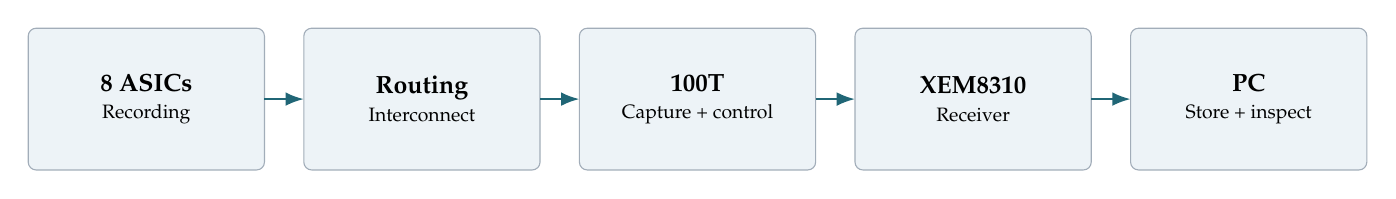
\begin{tikzpicture}[x=1mm,y=1mm,>=Latex]
\foreach \x/\title/\sub in {0/8 ASICs/Recording,35/Routing/Interconnect,70/100T/Capture + control,105/XEM8310/Receiver,140/PC/Store + inspect}{
\node[draw=muted!60,rounded corners=1mm,fill=paperblue,minimum width=30mm,minimum height=18mm,align=center,font=\small] at (\x,0) {\textbf{\title}\\[-1pt]{\scriptsize\sub}};}
\foreach \x in {15,50,85,120}\draw[->,teal,line width=.8pt] (\x,0)--(\x+5,0);
\end{tikzpicture}\end{center}
{\small\textbf{Figure 1.} Intended system path. This diagram describes the target behavior; full ASIC and cable assignments and end-to-end firmware are unfinished.}

\begingroup\fontsize{10}{12.5}\selectfont\setlength{\tabcolsep}{2.8pt}\renewcommand{\arraystretch}{1.12}
\begin{longtable}{@{}P{53mm}P{13mm}P{99mm}@{}}
\toprule \textbf{Function} & \textbf{Parts} & \textbf{What the group contributes} \\ \midrule
\endfirsthead\toprule \textbf{Function} & \textbf{Parts} & \textbf{What the group contributes} \\ \midrule
\endhead\midrule\multicolumn{3}{r}{\footnotesize Continued on next page}\endfoot\bottomrule\endlastfoot
FPGA logic & 1 & U1: programmable acquisition and control logic. \\
Four power rails & 39 & Four converters and their energy storage, voltage-setting and startup parts. \\
FPGA supply decoupling & 61 & Local and bulk supply capacitors around the FPGA power domains. \\
Boot memory & 11 & Flash memory and its local supply and signal-support parts. \\
System clock & 4 & The 32 MHz oscillator and its supply/edge support. \\
Configuration and JTAG & 11 & Startup straps, pull-ups and JTAG support. \\
External connections & 3 & J4 powered cable; J5/J6 two 60-contact mezzanines. \\
\end{longtable}\endgroup

\textbf{Why 130 parts around one chip?} The FPGA package contains the digital logic, but it still needs correct power, stable startup states, a configuration image, clocking and physical interfaces. Small supporting components provide those functions.

\textbf{Read a component reference.} U identifies an integrated circuit; C a capacitor; R a resistor; L an inductor; J a connector; Y the oscillator. For example, U1 is the FPGA, while R119 is a resistor in its reference-clock path. These letters are reference labels, not pin numbers.

\saybox{This is the interface between the recording-chip routing board and the downstream FPGA module. The surrounding parts make power, startup, timing and connection possible.}


\clearpage\section{Power: one cable input, four local supplies}\label{sec:power}

A \textbf{rail} is a named power-supply connection. The FPGA core, auxiliary circuits and I/O banks use different rails. A \textbf{bank} is a group of FPGA I/O pins sharing a supply and electrical constraints; it is not an independently programmable voltage source.

The current architecture proposes nominal 12 V at J4.19. Each TPS62135 converter and inductor steps that voltage down. The 1.5 V ASIC-facing and 2.5 V link-bank choices still require interface validation; they are not universal requirements of every Artix-7 application [1,2].
\begin{center}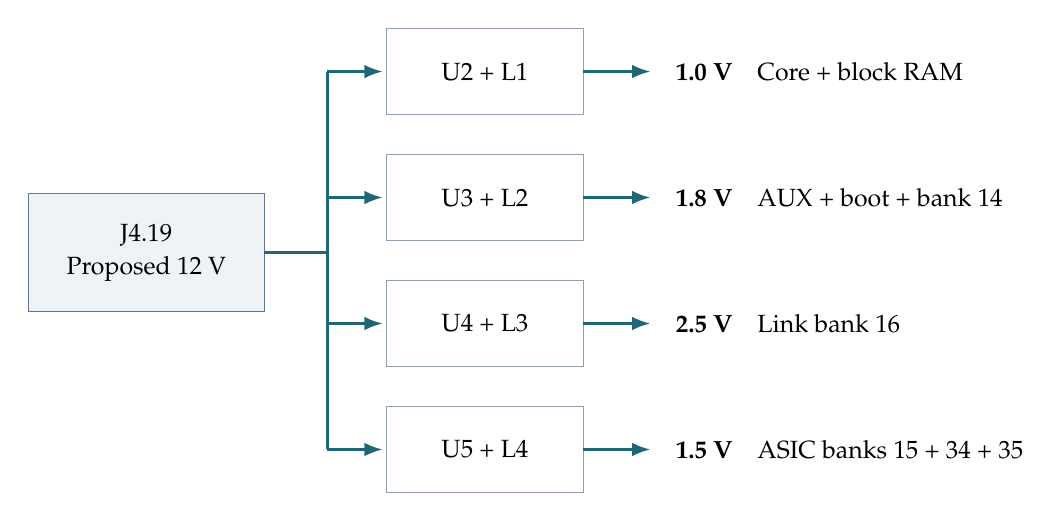
\begin{tikzpicture}[x=1mm,y=1mm,>=Latex]
\node[draw=muted,fill=paperblue,align=center,minimum width=30mm,minimum height=15mm] (input) at (15,-23) {\small J4.19\\\small Proposed 12 V};
\draw[teal,line width=1pt] (30,-23)--(38,-23);\draw[teal,line width=1pt] (38,0)--(38,-48);
\foreach \y/\id/\coil/\rail/\load in {0/U2/L1/1.0 V/Core + block RAM,-16/U3/L2/1.8 V/AUX + boot + bank 14,-32/U4/L3/2.5 V/Link bank 16,-48/U5/L4/1.5 V/ASIC banks 15 + 34 + 35}{
\draw[->,teal,line width=.8pt] (38,\y)--(45,\y);
\node[draw=muted!70,align=center,minimum width=25mm,minimum height=11mm] at (58,\y) {\small \id\ + \coil};
\draw[->,teal,line width=.8pt] (70.5,\y)--(79,\y);
\node[anchor=west,align=left,font=\small] at (81,\y) {\textbf{\rail}\quad \load};}
\end{tikzpicture}\end{center}
{\small\textbf{Figure 2.} Supply destinations. This is a functional diagram, not a routed power or enable diagram. R9 separates U2's local output from the core rail; R122 does the same for U3's distributed 1.8 V rail.}

\textbf{What each converter needs.} Its inductor transfers energy; input/output capacitors support the switching-current loops; a feedback divider sets the output; the soft-start network controls the startup transition. Placement and current-return paths matter as much as logical connectivity [1].

\textbf{Startup order.} The present enable chain is \nolinkurl{PG_CORE} $\rightarrow$ U3, then \nolinkurl{PG_AUX} $\rightarrow$ U4/U5. These two sequencing nets are connected in the saved checks. Startup and shutdown waveforms still need measurement. R12's \nolinkurl{PGOOD_IO} signal has no consumer.

\textbf{Why the local names differ.} U2's local sense node is \nolinkurl{VCORE_REG_1V025}; the distributed rail after R9 is \nolinkurl{VCCINT_1V0}. R9 and R122 are 15 milliohm isolation resistors, not zero-ohm jumpers. For illustration only, 1 A through 15 milliohm drops 15 mV; the actual load and copper loss need analysis. Do not bypass either resistor during routing.

\finding{The headboard does not yet have a completed input-protection solution. A powered cable and carrier must be designed and qualified; an unmodified XEM8310 is not established as this board's power source.}

\saybox{The cable voltage is converted into the rails required by our chosen core and interface architecture. Connected power-good wires do not yet prove correct power-up at the FPGA pins.}


\clearpage\section{Capacitors: why so many small parts?}\label{sec:caps}

A capacitor stores charge. Close to a switching load, it can supply a brief current pulse while the regulator and wider power network respond. \textbf{Decoupling} means providing that local supply support and limiting unwanted coupling through supply impedance.

There are \textbf{83 capacitors in the saved board}: 61 belong to the FPGA supply-decoupling group, and 22 support converters, cable entry, flash or oscillator circuits. The figure below illustrates a function, not a literal trace path.
\begin{center}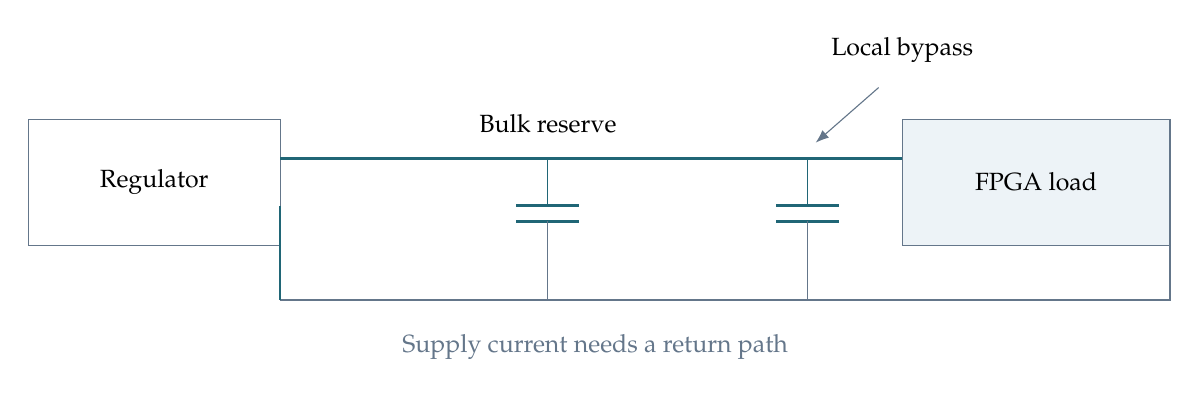
\begin{tikzpicture}[x=1mm,y=1mm,>=Latex]
\node[draw=muted,minimum width=32mm,minimum height=16mm,align=center] (reg) at (15,0) {\small Regulator};
\node[draw=muted,fill=paperblue,minimum width=34mm,minimum height=16mm,align=center] (load) at (127,0) {\small FPGA load};
\draw[teal,line width=1pt] (31,3)--(110,3);\draw[muted,line width=.8pt] (31,-15)--(144,-15)--(144,-8);
\draw[teal,line width=.8pt] (31,-3)--(31,-15);
\foreach \x in {65,98}{\draw[teal] (\x,3)--(\x,-3);\draw[teal,line width=1pt] (\x-4,-3)--(\x+4,-3);\draw[teal,line width=1pt] (\x-4,-5)--(\x+4,-5);\draw[muted] (\x,-5)--(\x,-15);}
\node[font=\small,anchor=south] at (65,5) {Bulk reserve};\node[font=\small,anchor=south] at (110,14) {Local bypass};
\draw[->,muted] (107,12)--(99,5);\node[font=\small,text=muted] at (71,-21) {Supply current needs a return path};
\end{tikzpicture}\end{center}

\begingroup\fontsize{9.5}{12.0}\selectfont\setlength{\tabcolsep}{2.8pt}\renewcommand{\arraystretch}{1.12}
\begin{longtable}{@{}P{48mm}P{97mm}P{18mm}@{}}
\toprule \textbf{FPGA domain} & \textbf{Capacitors} & \textbf{Count} \\ \midrule
\endfirsthead\toprule \textbf{FPGA domain} & \textbf{Capacitors} & \textbf{Count} \\ \midrule
\endhead\midrule\multicolumn{3}{r}{\footnotesize Continued on next page}\endfoot\bottomrule\endlastfoot
Core & C20, C22-C35 & 15 \\
Block RAM & C21, C36, C37 & 3 \\
Auxiliary & C40-C46 & 7 \\
Configuration bank 0 & C50 & 1 \\
Bank 14 & C51-C56, C92 & 7 \\
Bank 16 & C57-C63 & 7 \\
Banks 15 / 34 / 35 & C64-C81 & 18 \\
Shared ASIC-bank bulk & C82 & 1 \\
XADC-related supply & C90, C91 & 2 \\
\end{longtable}\endgroup

\textbf{Why different values and locations?} The entire mounted network has capacitance, resistance and inductance. Larger nominal capacitance is not automatically better at every frequency, and a long connection can reduce the value of a nearby capacitor. Two parts on the same net can serve different current paths [3].

\textbf{Can we remove some?} The required function is an adequate power-distribution network. The exact count is not proven minimal. Reduction needs an application load model, effective capacitance, impedance/placement analysis and suitable measurements. C92 supports bank 14 after the voltage-domain split; removing it simply because other 1.8 V capacitors exist is not justified. C21's recorded part choice also needs an orderable replacement review.

\saybox{These are local energy reserves, not decorative extras. We can optimize the network, but we need evidence that the FPGA supply remains within limits after the change.}


\clearpage\section{Startup, memory, clock and programming}\label{sec:boot}

\textbf{Configuration} is loading the FPGA's logic design. It is separate from the application data captured later. U6 is the 1.8 V MX25U12835F flash that stores a configuration image for independent startup [4,5]. Removing it requires another configuration source at every power-up.

\begin{center}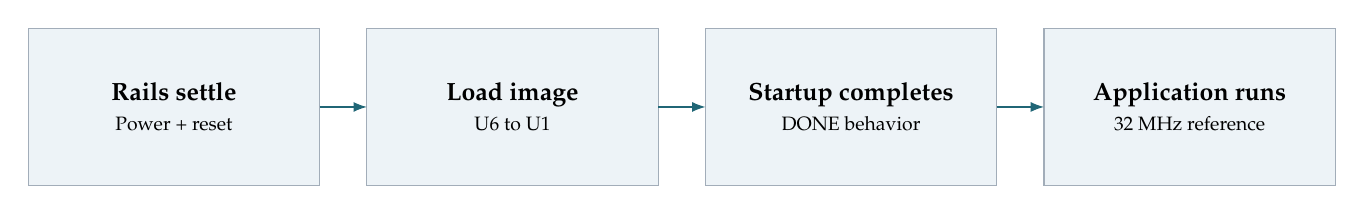
\begin{tikzpicture}[x=1mm,y=1mm,>=Latex]
\foreach \x/\title/\sub in {0/Rails settle/Power + reset,43/Load image/U6 to U1,86/Startup completes/DONE behavior,129/Application runs/32 MHz reference}{\node[draw=muted!60,fill=paperblue,minimum width=37mm,minimum height=20mm,align=center,font=\small] at (\x,0) {\textbf{\title}\\{\scriptsize\sub}};}
\foreach \x in {18.5,61.5,104.5}\draw[->,teal] (\x,0)--(\x+6,0);
\end{tikzpicture}\end{center}
{\small\textbf{Figure 3.} Conceptual startup sequence, not measured timing. The oscillator can run before the application; it is not switched on by DONE in this circuit.}

\begingroup\fontsize{9.3}{11.8}\selectfont\setlength{\tabcolsep}{2.8pt}\renewcommand{\arraystretch}{1.12}
\begin{longtable}{@{}P{35mm}P{58mm}P{73mm}@{}}
\toprule \textbf{Parts} & \textbf{Purpose} & \textbf{What to remember} \\ \midrule
\endfirsthead\toprule \textbf{Parts} & \textbf{Purpose} & \textbf{What to remember} \\ \midrule
\endhead\midrule\multicolumn{3}{r}{\footnotesize Continued on next page}\endfoot\bottomrule\endlastfoot
U6; C100/C101 & Boot storage and local supply support & A stored image and verified flash/configuration settings are still needed. \\
R100-R107 & Flash startup levels and signal paths & U6.7 is RESET/SIO3 for this exact part. Zero-ohm links still carry a connection. \\
Y1; C102/C103; R119 & 1.8 V oscillator, bypass and clock edge & 32 MHz reference; damping value needs signal-integrity review. \\
R108 / R109 & PROGRAM\_B / INIT\_B pull-ups & Keep the specified external pull-up functions. \\
R110 & Additional DONE pull-up & Conditional: DONE has an internal pull-up; review loading/startup before removal. \\
R111-R114 & SPI mode and PUDC\_B startup straps & Keep the required states; reviewed copper ties could replace some resistor footprints. \\
R115-R118; J4 & JTAG bias and TDO path & Dedicated FPGA programming pins share the custom cable connector. \\
\end{longtable}\endgroup

\textbf{Read one actual signal path.} Y1.3 and R119.1 share \nolinkurl{OSC_32M_RAW}. R119.2 and U1.P17 share \nolinkurl{CLK_32MHZ}. The resistor deliberately separates two net names. The signal nets are connected in the saved native check; rail/ground completion and waveform quality remain open.

\textbf{A pull-up is not a wire replacement.} It biases a signal high while allowing a device to drive it low. A fixed mode strap has a different role. That is why all startup resistors cannot be removed using one general rule [4].

\saybox{Flash stores the design, the oscillator supplies a time reference, and startup/JTAG parts make configuration predictable and accessible. No cold boot or programming test has yet been demonstrated on this board.}


\clearpage\section{The 117 signals and three connectors}\label{sec:connectors}

The corrected ASIC interface budget is \textbf{117 logical signals}. The 88-output group consists of eight sets of 11: each set includes eight data outputs, a returned clock, READ and SYNC. It is not 88 independent sampled data bits. Gerald's tutorial establishes useful framing, but electrical limits and several timing details remain unresolved [8].

\begingroup\fontsize{9.3}{11.8}\selectfont\setlength{\tabcolsep}{2.8pt}\renewcommand{\arraystretch}{1.12}
\begin{longtable}{@{}P{53mm}P{14mm}P{99mm}@{}}
\toprule \textbf{Signal group} & \textbf{Count} & \textbf{Interpretation} \\ \midrule
\endfirsthead\toprule \textbf{Signal group} & \textbf{Count} & \textbf{Interpretation} \\ \midrule
\endhead\midrule\multicolumn{3}{r}{\footnotesize Continued on next page}\endfoot\bottomrule\endlastfoot
ASIC output/interface lines & 88 & 8 ASICs x 11; includes data and associated timing/handshake. \\
SPI L/R streams & 12 & Stimulation and non-stimulation configuration data streams. \\
Shared controls & 9 & CHIP\_RESET, AC\_IN, IMP\_TST, FE\_RESET, SPI\_LATCH, STIM\_CLK, STIM\_START, STIM\_EN, STIM\_CHB. \\
Board clocks & 4 & One recording-board clock per board. \\
Additional SPI clocks & 4 & Correction to the original 113-signal count. \\
Total & 117 & Excludes grounds, power and shielding. \\
\end{longtable}\endgroup

\textbf{J5 and J6: routing-board connection.} Two 60-contact mezzanines provide 120 numbered signal contacts, plus separate ground-blade lands. The allocation proposal is 117 signals plus three reserved contacts. All 120 remain unassigned in the native design, so those three are not yet implemented permanent spares.

\textbf{J4: powered cable and JTAG.} This micro-HDMI-style connector has a custom electrical assignment. It is incompatible with ordinary HDMI equipment. The eight lane contacts are reserved for a proposed data link; they are still unassigned in CAD.

\begingroup\fontsize{9.2}{11.7}\selectfont\setlength{\tabcolsep}{2.8pt}\renewcommand{\arraystretch}{1.12}
\begin{longtable}{@{}P{40mm}P{51mm}P{75mm}@{}}
\toprule \textbf{J4 contacts} & \textbf{Saved assignment} & \textbf{Meaning} \\ \midrule
\endfirsthead\toprule \textbf{J4 contacts} & \textbf{Saved assignment} & \textbf{Meaning} \\ \midrule
\endhead\midrule\multicolumn{3}{r}{\footnotesize Continued on next page}\endfoot\bottomrule\endlastfoot
19 & LINK\_12V & Proposed nominal 12 V input. \\
1 & VCCAUX\_1V8 & 1.8 V target-voltage reference for programming. \\
2 / 15 / 17 / 18 & TMS / TDI / TCK / TDO & Dedicated target JTAG connections. \\
16; 4 / 7 / 10 / 13; SH & GND & DC return, pair shields and shell. \\
3/5; 6/8; 9/11; 12/14 & Unassigned & Four proposed differential-pair positions. \\
\end{longtable}\endgroup

\finding{The XEM8310 carrier contacts, cable continuity, voltage/current limits, link timing, termination and target-JTAG bridge remain to be designed or qualified. AC\_IN and IMP\_TST do not yet have established pad functions and safe electrical limits.}

\saybox{J5 and J6 carry our ASIC interface; J4 combines power and programming with reserved data contacts. None of these three connectors is an unexplained extra header.}


\clearpage\section{Unused function does not mean leave it open}\label{sec:pinstatus}

A \textbf{pin} is an electrical terminal; a \textbf{pad} is its physical copper landing. Some ground and shell terminals have multiple pads. A \textbf{net} names terminals intended to be electrically joined. A \textbf{via} connects copper between board layers.

The current 762 numbered endpoints comprise 425 assigned endpoints, 331 unassigned endpoints and six marked NC (no-connect) in the saved CAD. This report adds the electrical review overlay below. It does not silently turn unfinished interfaces into approved no-connects.

\begingroup\fontsize{9.7}{12.2}\selectfont\setlength{\tabcolsep}{2.8pt}\renewcommand{\arraystretch}{1.12}
\begin{longtable}{@{}P{14mm}P{50mm}P{102mm}@{}}
\toprule \textbf{Code} & \textbf{Read it as} & \textbf{What it establishes} \\ \midrule
\endfirsthead\toprule \textbf{Code} & \textbf{Read it as} & \textbf{What it establishes} \\ \midrule
\endhead\midrule\multicolumn{3}{r}{\footnotesize Continued on next page}\endfoot\bottomrule\endlastfoot
C & Assigned; whole net connected & Native connectivity only, not waveform quality or working hardware. \\
P & Assigned; net has gaps & At least one gap exists somewhere on this net. This individual pad may already be connected locally. \\
U & Awaiting assignment & A final signal/net has not been implemented. Do not call every U pin a permanent spare. \\
G & Ground required; saved NC & U1.L9 DXN\_0 and U1.L10 DXP\_0 require GND per AMD UG475. \\
R & Grounding review; saved NC & U2-U5 pin 4 FB2: unused switched-divider outputs. TI single-divider example grounds them. \\
\end{longtable}\endgroup

\finding{\textbf{U1.L9 and U1.L10 need correction.} The temperature-diode function is unused, but AMD's package guidance requires the pins tied to GND [7]. Their current NC markers are incorrect final wiring. The source PCB remains unchanged in this report.}

\textbf{FB2 is a different case.} U2.4, U3.4, U4.4 and U5.4 are optional switched-feedback outputs. No divider branch is attached here. TI's Figure 5 grounds FB2 in its single-divider circuit; this audit therefore marks a grounding review, without pretending the current NC treatment has explicit manufacturer approval [1].

\textbf{331 unassigned endpoints are separate from 146 routing gaps.} The unassigned set is 203 U1 user-I/O balls + 120 J5/J6 contacts + eight J4 lane contacts. A signal with no assignment cannot be counted as a missing connection on an already assigned net.

\textbf{Do not double-count physical lands.} The 762 electrical endpoint IDs represent 771 numbered pad records. Another 40 unnumbered pad records bring the physical total to 811. The 130 components are neither 130 pins nor 130 nets.

\saybox{I use one label for unassigned signals, another for incomplete copper, and explicit correction labels for unused functions that still need a ground connection or review.}


\clearpage\section{Read the FPGA ball map}\label{sec:ballmap}

Every one of U1's 324 balls is shown below using native pad coordinates, viewed from the front of the PCB. A1 is at the top left in this saved layout. This is not a bottom-of-package or connector mating-face drawing. Each circle shows its ball name and the status code defined on page~\pageref{sec:pinstatus}.

\begin{center}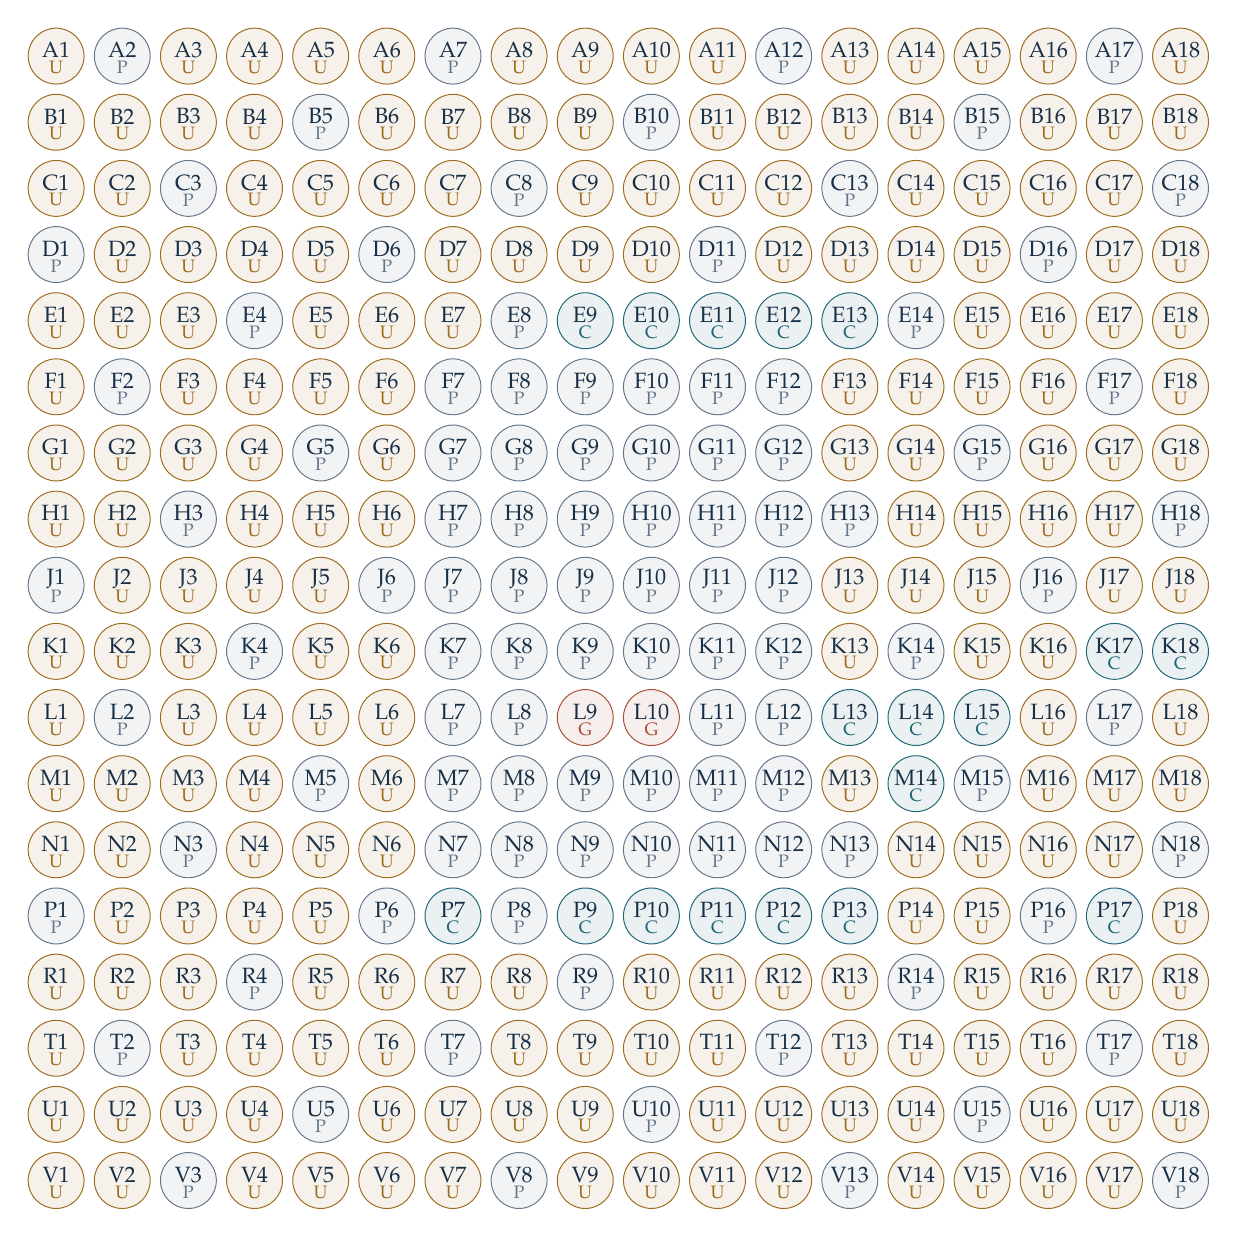
\begin{tikzpicture}[x=1mm,y=-1mm]
\draw[fill=amber!9,draw=amber,line width=.35pt] (0.000,0.000) circle (3.55);
\node[font=\fontsize{8}{8.5}\selectfont,text=navy] at (0.000,-0.750) {A1};
\node[font=\fontsize{6.5}{7}\selectfont,text=amber] at (0.000,1.450) {U};
\draw[fill=amber!9,draw=amber,line width=.35pt] (75.600,0.000) circle (3.55);
\node[font=\fontsize{8}{8.5}\selectfont,text=navy] at (75.600,-0.750) {A10};
\node[font=\fontsize{6.5}{7}\selectfont,text=amber] at (75.600,1.450) {U};
\draw[fill=amber!9,draw=amber,line width=.35pt] (84.000,0.000) circle (3.55);
\node[font=\fontsize{8}{8.5}\selectfont,text=navy] at (84.000,-0.750) {A11};
\node[font=\fontsize{6.5}{7}\selectfont,text=amber] at (84.000,1.450) {U};
\draw[fill=muted!9,draw=muted,line width=.35pt] (92.400,0.000) circle (3.55);
\node[font=\fontsize{8}{8.5}\selectfont,text=navy] at (92.400,-0.750) {A12};
\node[font=\fontsize{6.5}{7}\selectfont,text=muted] at (92.400,1.450) {P};
\draw[fill=amber!9,draw=amber,line width=.35pt] (100.800,0.000) circle (3.55);
\node[font=\fontsize{8}{8.5}\selectfont,text=navy] at (100.800,-0.750) {A13};
\node[font=\fontsize{6.5}{7}\selectfont,text=amber] at (100.800,1.450) {U};
\draw[fill=amber!9,draw=amber,line width=.35pt] (109.200,0.000) circle (3.55);
\node[font=\fontsize{8}{8.5}\selectfont,text=navy] at (109.200,-0.750) {A14};
\node[font=\fontsize{6.5}{7}\selectfont,text=amber] at (109.200,1.450) {U};
\draw[fill=amber!9,draw=amber,line width=.35pt] (117.600,0.000) circle (3.55);
\node[font=\fontsize{8}{8.5}\selectfont,text=navy] at (117.600,-0.750) {A15};
\node[font=\fontsize{6.5}{7}\selectfont,text=amber] at (117.600,1.450) {U};
\draw[fill=amber!9,draw=amber,line width=.35pt] (126.000,0.000) circle (3.55);
\node[font=\fontsize{8}{8.5}\selectfont,text=navy] at (126.000,-0.750) {A16};
\node[font=\fontsize{6.5}{7}\selectfont,text=amber] at (126.000,1.450) {U};
\draw[fill=muted!9,draw=muted,line width=.35pt] (134.400,0.000) circle (3.55);
\node[font=\fontsize{8}{8.5}\selectfont,text=navy] at (134.400,-0.750) {A17};
\node[font=\fontsize{6.5}{7}\selectfont,text=muted] at (134.400,1.450) {P};
\draw[fill=amber!9,draw=amber,line width=.35pt] (142.800,0.000) circle (3.55);
\node[font=\fontsize{8}{8.5}\selectfont,text=navy] at (142.800,-0.750) {A18};
\node[font=\fontsize{6.5}{7}\selectfont,text=amber] at (142.800,1.450) {U};
\draw[fill=muted!9,draw=muted,line width=.35pt] (8.400,0.000) circle (3.55);
\node[font=\fontsize{8}{8.5}\selectfont,text=navy] at (8.400,-0.750) {A2};
\node[font=\fontsize{6.5}{7}\selectfont,text=muted] at (8.400,1.450) {P};
\draw[fill=amber!9,draw=amber,line width=.35pt] (16.800,0.000) circle (3.55);
\node[font=\fontsize{8}{8.5}\selectfont,text=navy] at (16.800,-0.750) {A3};
\node[font=\fontsize{6.5}{7}\selectfont,text=amber] at (16.800,1.450) {U};
\draw[fill=amber!9,draw=amber,line width=.35pt] (25.200,0.000) circle (3.55);
\node[font=\fontsize{8}{8.5}\selectfont,text=navy] at (25.200,-0.750) {A4};
\node[font=\fontsize{6.5}{7}\selectfont,text=amber] at (25.200,1.450) {U};
\draw[fill=amber!9,draw=amber,line width=.35pt] (33.600,0.000) circle (3.55);
\node[font=\fontsize{8}{8.5}\selectfont,text=navy] at (33.600,-0.750) {A5};
\node[font=\fontsize{6.5}{7}\selectfont,text=amber] at (33.600,1.450) {U};
\draw[fill=amber!9,draw=amber,line width=.35pt] (42.000,0.000) circle (3.55);
\node[font=\fontsize{8}{8.5}\selectfont,text=navy] at (42.000,-0.750) {A6};
\node[font=\fontsize{6.5}{7}\selectfont,text=amber] at (42.000,1.450) {U};
\draw[fill=muted!9,draw=muted,line width=.35pt] (50.400,0.000) circle (3.55);
\node[font=\fontsize{8}{8.5}\selectfont,text=navy] at (50.400,-0.750) {A7};
\node[font=\fontsize{6.5}{7}\selectfont,text=muted] at (50.400,1.450) {P};
\draw[fill=amber!9,draw=amber,line width=.35pt] (58.800,0.000) circle (3.55);
\node[font=\fontsize{8}{8.5}\selectfont,text=navy] at (58.800,-0.750) {A8};
\node[font=\fontsize{6.5}{7}\selectfont,text=amber] at (58.800,1.450) {U};
\draw[fill=amber!9,draw=amber,line width=.35pt] (67.200,0.000) circle (3.55);
\node[font=\fontsize{8}{8.5}\selectfont,text=navy] at (67.200,-0.750) {A9};
\node[font=\fontsize{6.5}{7}\selectfont,text=amber] at (67.200,1.450) {U};
\draw[fill=amber!9,draw=amber,line width=.35pt] (0.000,8.400) circle (3.55);
\node[font=\fontsize{8}{8.5}\selectfont,text=navy] at (0.000,7.650) {B1};
\node[font=\fontsize{6.5}{7}\selectfont,text=amber] at (0.000,9.850) {U};
\draw[fill=muted!9,draw=muted,line width=.35pt] (75.600,8.400) circle (3.55);
\node[font=\fontsize{8}{8.5}\selectfont,text=navy] at (75.600,7.650) {B10};
\node[font=\fontsize{6.5}{7}\selectfont,text=muted] at (75.600,9.850) {P};
\draw[fill=amber!9,draw=amber,line width=.35pt] (84.000,8.400) circle (3.55);
\node[font=\fontsize{8}{8.5}\selectfont,text=navy] at (84.000,7.650) {B11};
\node[font=\fontsize{6.5}{7}\selectfont,text=amber] at (84.000,9.850) {U};
\draw[fill=amber!9,draw=amber,line width=.35pt] (92.400,8.400) circle (3.55);
\node[font=\fontsize{8}{8.5}\selectfont,text=navy] at (92.400,7.650) {B12};
\node[font=\fontsize{6.5}{7}\selectfont,text=amber] at (92.400,9.850) {U};
\draw[fill=amber!9,draw=amber,line width=.35pt] (100.800,8.400) circle (3.55);
\node[font=\fontsize{8}{8.5}\selectfont,text=navy] at (100.800,7.650) {B13};
\node[font=\fontsize{6.5}{7}\selectfont,text=amber] at (100.800,9.850) {U};
\draw[fill=amber!9,draw=amber,line width=.35pt] (109.200,8.400) circle (3.55);
\node[font=\fontsize{8}{8.5}\selectfont,text=navy] at (109.200,7.650) {B14};
\node[font=\fontsize{6.5}{7}\selectfont,text=amber] at (109.200,9.850) {U};
\draw[fill=muted!9,draw=muted,line width=.35pt] (117.600,8.400) circle (3.55);
\node[font=\fontsize{8}{8.5}\selectfont,text=navy] at (117.600,7.650) {B15};
\node[font=\fontsize{6.5}{7}\selectfont,text=muted] at (117.600,9.850) {P};
\draw[fill=amber!9,draw=amber,line width=.35pt] (126.000,8.400) circle (3.55);
\node[font=\fontsize{8}{8.5}\selectfont,text=navy] at (126.000,7.650) {B16};
\node[font=\fontsize{6.5}{7}\selectfont,text=amber] at (126.000,9.850) {U};
\draw[fill=amber!9,draw=amber,line width=.35pt] (134.400,8.400) circle (3.55);
\node[font=\fontsize{8}{8.5}\selectfont,text=navy] at (134.400,7.650) {B17};
\node[font=\fontsize{6.5}{7}\selectfont,text=amber] at (134.400,9.850) {U};
\draw[fill=amber!9,draw=amber,line width=.35pt] (142.800,8.400) circle (3.55);
\node[font=\fontsize{8}{8.5}\selectfont,text=navy] at (142.800,7.650) {B18};
\node[font=\fontsize{6.5}{7}\selectfont,text=amber] at (142.800,9.850) {U};
\draw[fill=amber!9,draw=amber,line width=.35pt] (8.400,8.400) circle (3.55);
\node[font=\fontsize{8}{8.5}\selectfont,text=navy] at (8.400,7.650) {B2};
\node[font=\fontsize{6.5}{7}\selectfont,text=amber] at (8.400,9.850) {U};
\draw[fill=amber!9,draw=amber,line width=.35pt] (16.800,8.400) circle (3.55);
\node[font=\fontsize{8}{8.5}\selectfont,text=navy] at (16.800,7.650) {B3};
\node[font=\fontsize{6.5}{7}\selectfont,text=amber] at (16.800,9.850) {U};
\draw[fill=amber!9,draw=amber,line width=.35pt] (25.200,8.400) circle (3.55);
\node[font=\fontsize{8}{8.5}\selectfont,text=navy] at (25.200,7.650) {B4};
\node[font=\fontsize{6.5}{7}\selectfont,text=amber] at (25.200,9.850) {U};
\draw[fill=muted!9,draw=muted,line width=.35pt] (33.600,8.400) circle (3.55);
\node[font=\fontsize{8}{8.5}\selectfont,text=navy] at (33.600,7.650) {B5};
\node[font=\fontsize{6.5}{7}\selectfont,text=muted] at (33.600,9.850) {P};
\draw[fill=amber!9,draw=amber,line width=.35pt] (42.000,8.400) circle (3.55);
\node[font=\fontsize{8}{8.5}\selectfont,text=navy] at (42.000,7.650) {B6};
\node[font=\fontsize{6.5}{7}\selectfont,text=amber] at (42.000,9.850) {U};
\draw[fill=amber!9,draw=amber,line width=.35pt] (50.400,8.400) circle (3.55);
\node[font=\fontsize{8}{8.5}\selectfont,text=navy] at (50.400,7.650) {B7};
\node[font=\fontsize{6.5}{7}\selectfont,text=amber] at (50.400,9.850) {U};
\draw[fill=amber!9,draw=amber,line width=.35pt] (58.800,8.400) circle (3.55);
\node[font=\fontsize{8}{8.5}\selectfont,text=navy] at (58.800,7.650) {B8};
\node[font=\fontsize{6.5}{7}\selectfont,text=amber] at (58.800,9.850) {U};
\draw[fill=amber!9,draw=amber,line width=.35pt] (67.200,8.400) circle (3.55);
\node[font=\fontsize{8}{8.5}\selectfont,text=navy] at (67.200,7.650) {B9};
\node[font=\fontsize{6.5}{7}\selectfont,text=amber] at (67.200,9.850) {U};
\draw[fill=amber!9,draw=amber,line width=.35pt] (0.000,16.800) circle (3.55);
\node[font=\fontsize{8}{8.5}\selectfont,text=navy] at (0.000,16.050) {C1};
\node[font=\fontsize{6.5}{7}\selectfont,text=amber] at (0.000,18.250) {U};
\draw[fill=amber!9,draw=amber,line width=.35pt] (75.600,16.800) circle (3.55);
\node[font=\fontsize{8}{8.5}\selectfont,text=navy] at (75.600,16.050) {C10};
\node[font=\fontsize{6.5}{7}\selectfont,text=amber] at (75.600,18.250) {U};
\draw[fill=amber!9,draw=amber,line width=.35pt] (84.000,16.800) circle (3.55);
\node[font=\fontsize{8}{8.5}\selectfont,text=navy] at (84.000,16.050) {C11};
\node[font=\fontsize{6.5}{7}\selectfont,text=amber] at (84.000,18.250) {U};
\draw[fill=amber!9,draw=amber,line width=.35pt] (92.400,16.800) circle (3.55);
\node[font=\fontsize{8}{8.5}\selectfont,text=navy] at (92.400,16.050) {C12};
\node[font=\fontsize{6.5}{7}\selectfont,text=amber] at (92.400,18.250) {U};
\draw[fill=muted!9,draw=muted,line width=.35pt] (100.800,16.800) circle (3.55);
\node[font=\fontsize{8}{8.5}\selectfont,text=navy] at (100.800,16.050) {C13};
\node[font=\fontsize{6.5}{7}\selectfont,text=muted] at (100.800,18.250) {P};
\draw[fill=amber!9,draw=amber,line width=.35pt] (109.200,16.800) circle (3.55);
\node[font=\fontsize{8}{8.5}\selectfont,text=navy] at (109.200,16.050) {C14};
\node[font=\fontsize{6.5}{7}\selectfont,text=amber] at (109.200,18.250) {U};
\draw[fill=amber!9,draw=amber,line width=.35pt] (117.600,16.800) circle (3.55);
\node[font=\fontsize{8}{8.5}\selectfont,text=navy] at (117.600,16.050) {C15};
\node[font=\fontsize{6.5}{7}\selectfont,text=amber] at (117.600,18.250) {U};
\draw[fill=amber!9,draw=amber,line width=.35pt] (126.000,16.800) circle (3.55);
\node[font=\fontsize{8}{8.5}\selectfont,text=navy] at (126.000,16.050) {C16};
\node[font=\fontsize{6.5}{7}\selectfont,text=amber] at (126.000,18.250) {U};
\draw[fill=amber!9,draw=amber,line width=.35pt] (134.400,16.800) circle (3.55);
\node[font=\fontsize{8}{8.5}\selectfont,text=navy] at (134.400,16.050) {C17};
\node[font=\fontsize{6.5}{7}\selectfont,text=amber] at (134.400,18.250) {U};
\draw[fill=muted!9,draw=muted,line width=.35pt] (142.800,16.800) circle (3.55);
\node[font=\fontsize{8}{8.5}\selectfont,text=navy] at (142.800,16.050) {C18};
\node[font=\fontsize{6.5}{7}\selectfont,text=muted] at (142.800,18.250) {P};
\draw[fill=amber!9,draw=amber,line width=.35pt] (8.400,16.800) circle (3.55);
\node[font=\fontsize{8}{8.5}\selectfont,text=navy] at (8.400,16.050) {C2};
\node[font=\fontsize{6.5}{7}\selectfont,text=amber] at (8.400,18.250) {U};
\draw[fill=muted!9,draw=muted,line width=.35pt] (16.800,16.800) circle (3.55);
\node[font=\fontsize{8}{8.5}\selectfont,text=navy] at (16.800,16.050) {C3};
\node[font=\fontsize{6.5}{7}\selectfont,text=muted] at (16.800,18.250) {P};
\draw[fill=amber!9,draw=amber,line width=.35pt] (25.200,16.800) circle (3.55);
\node[font=\fontsize{8}{8.5}\selectfont,text=navy] at (25.200,16.050) {C4};
\node[font=\fontsize{6.5}{7}\selectfont,text=amber] at (25.200,18.250) {U};
\draw[fill=amber!9,draw=amber,line width=.35pt] (33.600,16.800) circle (3.55);
\node[font=\fontsize{8}{8.5}\selectfont,text=navy] at (33.600,16.050) {C5};
\node[font=\fontsize{6.5}{7}\selectfont,text=amber] at (33.600,18.250) {U};
\draw[fill=amber!9,draw=amber,line width=.35pt] (42.000,16.800) circle (3.55);
\node[font=\fontsize{8}{8.5}\selectfont,text=navy] at (42.000,16.050) {C6};
\node[font=\fontsize{6.5}{7}\selectfont,text=amber] at (42.000,18.250) {U};
\draw[fill=amber!9,draw=amber,line width=.35pt] (50.400,16.800) circle (3.55);
\node[font=\fontsize{8}{8.5}\selectfont,text=navy] at (50.400,16.050) {C7};
\node[font=\fontsize{6.5}{7}\selectfont,text=amber] at (50.400,18.250) {U};
\draw[fill=muted!9,draw=muted,line width=.35pt] (58.800,16.800) circle (3.55);
\node[font=\fontsize{8}{8.5}\selectfont,text=navy] at (58.800,16.050) {C8};
\node[font=\fontsize{6.5}{7}\selectfont,text=muted] at (58.800,18.250) {P};
\draw[fill=amber!9,draw=amber,line width=.35pt] (67.200,16.800) circle (3.55);
\node[font=\fontsize{8}{8.5}\selectfont,text=navy] at (67.200,16.050) {C9};
\node[font=\fontsize{6.5}{7}\selectfont,text=amber] at (67.200,18.250) {U};
\draw[fill=muted!9,draw=muted,line width=.35pt] (0.000,25.200) circle (3.55);
\node[font=\fontsize{8}{8.5}\selectfont,text=navy] at (0.000,24.450) {D1};
\node[font=\fontsize{6.5}{7}\selectfont,text=muted] at (0.000,26.650) {P};
\draw[fill=amber!9,draw=amber,line width=.35pt] (75.600,25.200) circle (3.55);
\node[font=\fontsize{8}{8.5}\selectfont,text=navy] at (75.600,24.450) {D10};
\node[font=\fontsize{6.5}{7}\selectfont,text=amber] at (75.600,26.650) {U};
\draw[fill=muted!9,draw=muted,line width=.35pt] (84.000,25.200) circle (3.55);
\node[font=\fontsize{8}{8.5}\selectfont,text=navy] at (84.000,24.450) {D11};
\node[font=\fontsize{6.5}{7}\selectfont,text=muted] at (84.000,26.650) {P};
\draw[fill=amber!9,draw=amber,line width=.35pt] (92.400,25.200) circle (3.55);
\node[font=\fontsize{8}{8.5}\selectfont,text=navy] at (92.400,24.450) {D12};
\node[font=\fontsize{6.5}{7}\selectfont,text=amber] at (92.400,26.650) {U};
\draw[fill=amber!9,draw=amber,line width=.35pt] (100.800,25.200) circle (3.55);
\node[font=\fontsize{8}{8.5}\selectfont,text=navy] at (100.800,24.450) {D13};
\node[font=\fontsize{6.5}{7}\selectfont,text=amber] at (100.800,26.650) {U};
\draw[fill=amber!9,draw=amber,line width=.35pt] (109.200,25.200) circle (3.55);
\node[font=\fontsize{8}{8.5}\selectfont,text=navy] at (109.200,24.450) {D14};
\node[font=\fontsize{6.5}{7}\selectfont,text=amber] at (109.200,26.650) {U};
\draw[fill=amber!9,draw=amber,line width=.35pt] (117.600,25.200) circle (3.55);
\node[font=\fontsize{8}{8.5}\selectfont,text=navy] at (117.600,24.450) {D15};
\node[font=\fontsize{6.5}{7}\selectfont,text=amber] at (117.600,26.650) {U};
\draw[fill=muted!9,draw=muted,line width=.35pt] (126.000,25.200) circle (3.55);
\node[font=\fontsize{8}{8.5}\selectfont,text=navy] at (126.000,24.450) {D16};
\node[font=\fontsize{6.5}{7}\selectfont,text=muted] at (126.000,26.650) {P};
\draw[fill=amber!9,draw=amber,line width=.35pt] (134.400,25.200) circle (3.55);
\node[font=\fontsize{8}{8.5}\selectfont,text=navy] at (134.400,24.450) {D17};
\node[font=\fontsize{6.5}{7}\selectfont,text=amber] at (134.400,26.650) {U};
\draw[fill=amber!9,draw=amber,line width=.35pt] (142.800,25.200) circle (3.55);
\node[font=\fontsize{8}{8.5}\selectfont,text=navy] at (142.800,24.450) {D18};
\node[font=\fontsize{6.5}{7}\selectfont,text=amber] at (142.800,26.650) {U};
\draw[fill=amber!9,draw=amber,line width=.35pt] (8.400,25.200) circle (3.55);
\node[font=\fontsize{8}{8.5}\selectfont,text=navy] at (8.400,24.450) {D2};
\node[font=\fontsize{6.5}{7}\selectfont,text=amber] at (8.400,26.650) {U};
\draw[fill=amber!9,draw=amber,line width=.35pt] (16.800,25.200) circle (3.55);
\node[font=\fontsize{8}{8.5}\selectfont,text=navy] at (16.800,24.450) {D3};
\node[font=\fontsize{6.5}{7}\selectfont,text=amber] at (16.800,26.650) {U};
\draw[fill=amber!9,draw=amber,line width=.35pt] (25.200,25.200) circle (3.55);
\node[font=\fontsize{8}{8.5}\selectfont,text=navy] at (25.200,24.450) {D4};
\node[font=\fontsize{6.5}{7}\selectfont,text=amber] at (25.200,26.650) {U};
\draw[fill=amber!9,draw=amber,line width=.35pt] (33.600,25.200) circle (3.55);
\node[font=\fontsize{8}{8.5}\selectfont,text=navy] at (33.600,24.450) {D5};
\node[font=\fontsize{6.5}{7}\selectfont,text=amber] at (33.600,26.650) {U};
\draw[fill=muted!9,draw=muted,line width=.35pt] (42.000,25.200) circle (3.55);
\node[font=\fontsize{8}{8.5}\selectfont,text=navy] at (42.000,24.450) {D6};
\node[font=\fontsize{6.5}{7}\selectfont,text=muted] at (42.000,26.650) {P};
\draw[fill=amber!9,draw=amber,line width=.35pt] (50.400,25.200) circle (3.55);
\node[font=\fontsize{8}{8.5}\selectfont,text=navy] at (50.400,24.450) {D7};
\node[font=\fontsize{6.5}{7}\selectfont,text=amber] at (50.400,26.650) {U};
\draw[fill=amber!9,draw=amber,line width=.35pt] (58.800,25.200) circle (3.55);
\node[font=\fontsize{8}{8.5}\selectfont,text=navy] at (58.800,24.450) {D8};
\node[font=\fontsize{6.5}{7}\selectfont,text=amber] at (58.800,26.650) {U};
\draw[fill=amber!9,draw=amber,line width=.35pt] (67.200,25.200) circle (3.55);
\node[font=\fontsize{8}{8.5}\selectfont,text=navy] at (67.200,24.450) {D9};
\node[font=\fontsize{6.5}{7}\selectfont,text=amber] at (67.200,26.650) {U};
\draw[fill=amber!9,draw=amber,line width=.35pt] (0.000,33.600) circle (3.55);
\node[font=\fontsize{8}{8.5}\selectfont,text=navy] at (0.000,32.850) {E1};
\node[font=\fontsize{6.5}{7}\selectfont,text=amber] at (0.000,35.050) {U};
\draw[fill=teal!9,draw=teal,line width=.35pt] (75.600,33.600) circle (3.55);
\node[font=\fontsize{8}{8.5}\selectfont,text=navy] at (75.600,32.850) {E10};
\node[font=\fontsize{6.5}{7}\selectfont,text=teal] at (75.600,35.050) {C};
\draw[fill=teal!9,draw=teal,line width=.35pt] (84.000,33.600) circle (3.55);
\node[font=\fontsize{8}{8.5}\selectfont,text=navy] at (84.000,32.850) {E11};
\node[font=\fontsize{6.5}{7}\selectfont,text=teal] at (84.000,35.050) {C};
\draw[fill=teal!9,draw=teal,line width=.35pt] (92.400,33.600) circle (3.55);
\node[font=\fontsize{8}{8.5}\selectfont,text=navy] at (92.400,32.850) {E12};
\node[font=\fontsize{6.5}{7}\selectfont,text=teal] at (92.400,35.050) {C};
\draw[fill=teal!9,draw=teal,line width=.35pt] (100.800,33.600) circle (3.55);
\node[font=\fontsize{8}{8.5}\selectfont,text=navy] at (100.800,32.850) {E13};
\node[font=\fontsize{6.5}{7}\selectfont,text=teal] at (100.800,35.050) {C};
\draw[fill=muted!9,draw=muted,line width=.35pt] (109.200,33.600) circle (3.55);
\node[font=\fontsize{8}{8.5}\selectfont,text=navy] at (109.200,32.850) {E14};
\node[font=\fontsize{6.5}{7}\selectfont,text=muted] at (109.200,35.050) {P};
\draw[fill=amber!9,draw=amber,line width=.35pt] (117.600,33.600) circle (3.55);
\node[font=\fontsize{8}{8.5}\selectfont,text=navy] at (117.600,32.850) {E15};
\node[font=\fontsize{6.5}{7}\selectfont,text=amber] at (117.600,35.050) {U};
\draw[fill=amber!9,draw=amber,line width=.35pt] (126.000,33.600) circle (3.55);
\node[font=\fontsize{8}{8.5}\selectfont,text=navy] at (126.000,32.850) {E16};
\node[font=\fontsize{6.5}{7}\selectfont,text=amber] at (126.000,35.050) {U};
\draw[fill=amber!9,draw=amber,line width=.35pt] (134.400,33.600) circle (3.55);
\node[font=\fontsize{8}{8.5}\selectfont,text=navy] at (134.400,32.850) {E17};
\node[font=\fontsize{6.5}{7}\selectfont,text=amber] at (134.400,35.050) {U};
\draw[fill=amber!9,draw=amber,line width=.35pt] (142.800,33.600) circle (3.55);
\node[font=\fontsize{8}{8.5}\selectfont,text=navy] at (142.800,32.850) {E18};
\node[font=\fontsize{6.5}{7}\selectfont,text=amber] at (142.800,35.050) {U};
\draw[fill=amber!9,draw=amber,line width=.35pt] (8.400,33.600) circle (3.55);
\node[font=\fontsize{8}{8.5}\selectfont,text=navy] at (8.400,32.850) {E2};
\node[font=\fontsize{6.5}{7}\selectfont,text=amber] at (8.400,35.050) {U};
\draw[fill=amber!9,draw=amber,line width=.35pt] (16.800,33.600) circle (3.55);
\node[font=\fontsize{8}{8.5}\selectfont,text=navy] at (16.800,32.850) {E3};
\node[font=\fontsize{6.5}{7}\selectfont,text=amber] at (16.800,35.050) {U};
\draw[fill=muted!9,draw=muted,line width=.35pt] (25.200,33.600) circle (3.55);
\node[font=\fontsize{8}{8.5}\selectfont,text=navy] at (25.200,32.850) {E4};
\node[font=\fontsize{6.5}{7}\selectfont,text=muted] at (25.200,35.050) {P};
\draw[fill=amber!9,draw=amber,line width=.35pt] (33.600,33.600) circle (3.55);
\node[font=\fontsize{8}{8.5}\selectfont,text=navy] at (33.600,32.850) {E5};
\node[font=\fontsize{6.5}{7}\selectfont,text=amber] at (33.600,35.050) {U};
\draw[fill=amber!9,draw=amber,line width=.35pt] (42.000,33.600) circle (3.55);
\node[font=\fontsize{8}{8.5}\selectfont,text=navy] at (42.000,32.850) {E6};
\node[font=\fontsize{6.5}{7}\selectfont,text=amber] at (42.000,35.050) {U};
\draw[fill=amber!9,draw=amber,line width=.35pt] (50.400,33.600) circle (3.55);
\node[font=\fontsize{8}{8.5}\selectfont,text=navy] at (50.400,32.850) {E7};
\node[font=\fontsize{6.5}{7}\selectfont,text=amber] at (50.400,35.050) {U};
\draw[fill=muted!9,draw=muted,line width=.35pt] (58.800,33.600) circle (3.55);
\node[font=\fontsize{8}{8.5}\selectfont,text=navy] at (58.800,32.850) {E8};
\node[font=\fontsize{6.5}{7}\selectfont,text=muted] at (58.800,35.050) {P};
\draw[fill=teal!9,draw=teal,line width=.35pt] (67.200,33.600) circle (3.55);
\node[font=\fontsize{8}{8.5}\selectfont,text=navy] at (67.200,32.850) {E9};
\node[font=\fontsize{6.5}{7}\selectfont,text=teal] at (67.200,35.050) {C};
\draw[fill=amber!9,draw=amber,line width=.35pt] (0.000,42.000) circle (3.55);
\node[font=\fontsize{8}{8.5}\selectfont,text=navy] at (0.000,41.250) {F1};
\node[font=\fontsize{6.5}{7}\selectfont,text=amber] at (0.000,43.450) {U};
\draw[fill=muted!9,draw=muted,line width=.35pt] (75.600,42.000) circle (3.55);
\node[font=\fontsize{8}{8.5}\selectfont,text=navy] at (75.600,41.250) {F10};
\node[font=\fontsize{6.5}{7}\selectfont,text=muted] at (75.600,43.450) {P};
\draw[fill=muted!9,draw=muted,line width=.35pt] (84.000,42.000) circle (3.55);
\node[font=\fontsize{8}{8.5}\selectfont,text=navy] at (84.000,41.250) {F11};
\node[font=\fontsize{6.5}{7}\selectfont,text=muted] at (84.000,43.450) {P};
\draw[fill=muted!9,draw=muted,line width=.35pt] (92.400,42.000) circle (3.55);
\node[font=\fontsize{8}{8.5}\selectfont,text=navy] at (92.400,41.250) {F12};
\node[font=\fontsize{6.5}{7}\selectfont,text=muted] at (92.400,43.450) {P};
\draw[fill=amber!9,draw=amber,line width=.35pt] (100.800,42.000) circle (3.55);
\node[font=\fontsize{8}{8.5}\selectfont,text=navy] at (100.800,41.250) {F13};
\node[font=\fontsize{6.5}{7}\selectfont,text=amber] at (100.800,43.450) {U};
\draw[fill=amber!9,draw=amber,line width=.35pt] (109.200,42.000) circle (3.55);
\node[font=\fontsize{8}{8.5}\selectfont,text=navy] at (109.200,41.250) {F14};
\node[font=\fontsize{6.5}{7}\selectfont,text=amber] at (109.200,43.450) {U};
\draw[fill=amber!9,draw=amber,line width=.35pt] (117.600,42.000) circle (3.55);
\node[font=\fontsize{8}{8.5}\selectfont,text=navy] at (117.600,41.250) {F15};
\node[font=\fontsize{6.5}{7}\selectfont,text=amber] at (117.600,43.450) {U};
\draw[fill=amber!9,draw=amber,line width=.35pt] (126.000,42.000) circle (3.55);
\node[font=\fontsize{8}{8.5}\selectfont,text=navy] at (126.000,41.250) {F16};
\node[font=\fontsize{6.5}{7}\selectfont,text=amber] at (126.000,43.450) {U};
\draw[fill=muted!9,draw=muted,line width=.35pt] (134.400,42.000) circle (3.55);
\node[font=\fontsize{8}{8.5}\selectfont,text=navy] at (134.400,41.250) {F17};
\node[font=\fontsize{6.5}{7}\selectfont,text=muted] at (134.400,43.450) {P};
\draw[fill=amber!9,draw=amber,line width=.35pt] (142.800,42.000) circle (3.55);
\node[font=\fontsize{8}{8.5}\selectfont,text=navy] at (142.800,41.250) {F18};
\node[font=\fontsize{6.5}{7}\selectfont,text=amber] at (142.800,43.450) {U};
\draw[fill=muted!9,draw=muted,line width=.35pt] (8.400,42.000) circle (3.55);
\node[font=\fontsize{8}{8.5}\selectfont,text=navy] at (8.400,41.250) {F2};
\node[font=\fontsize{6.5}{7}\selectfont,text=muted] at (8.400,43.450) {P};
\draw[fill=amber!9,draw=amber,line width=.35pt] (16.800,42.000) circle (3.55);
\node[font=\fontsize{8}{8.5}\selectfont,text=navy] at (16.800,41.250) {F3};
\node[font=\fontsize{6.5}{7}\selectfont,text=amber] at (16.800,43.450) {U};
\draw[fill=amber!9,draw=amber,line width=.35pt] (25.200,42.000) circle (3.55);
\node[font=\fontsize{8}{8.5}\selectfont,text=navy] at (25.200,41.250) {F4};
\node[font=\fontsize{6.5}{7}\selectfont,text=amber] at (25.200,43.450) {U};
\draw[fill=amber!9,draw=amber,line width=.35pt] (33.600,42.000) circle (3.55);
\node[font=\fontsize{8}{8.5}\selectfont,text=navy] at (33.600,41.250) {F5};
\node[font=\fontsize{6.5}{7}\selectfont,text=amber] at (33.600,43.450) {U};
\draw[fill=amber!9,draw=amber,line width=.35pt] (42.000,42.000) circle (3.55);
\node[font=\fontsize{8}{8.5}\selectfont,text=navy] at (42.000,41.250) {F6};
\node[font=\fontsize{6.5}{7}\selectfont,text=amber] at (42.000,43.450) {U};
\draw[fill=muted!9,draw=muted,line width=.35pt] (50.400,42.000) circle (3.55);
\node[font=\fontsize{8}{8.5}\selectfont,text=navy] at (50.400,41.250) {F7};
\node[font=\fontsize{6.5}{7}\selectfont,text=muted] at (50.400,43.450) {P};
\draw[fill=muted!9,draw=muted,line width=.35pt] (58.800,42.000) circle (3.55);
\node[font=\fontsize{8}{8.5}\selectfont,text=navy] at (58.800,41.250) {F8};
\node[font=\fontsize{6.5}{7}\selectfont,text=muted] at (58.800,43.450) {P};
\draw[fill=muted!9,draw=muted,line width=.35pt] (67.200,42.000) circle (3.55);
\node[font=\fontsize{8}{8.5}\selectfont,text=navy] at (67.200,41.250) {F9};
\node[font=\fontsize{6.5}{7}\selectfont,text=muted] at (67.200,43.450) {P};
\draw[fill=amber!9,draw=amber,line width=.35pt] (0.000,50.400) circle (3.55);
\node[font=\fontsize{8}{8.5}\selectfont,text=navy] at (0.000,49.650) {G1};
\node[font=\fontsize{6.5}{7}\selectfont,text=amber] at (0.000,51.850) {U};
\draw[fill=muted!9,draw=muted,line width=.35pt] (75.600,50.400) circle (3.55);
\node[font=\fontsize{8}{8.5}\selectfont,text=navy] at (75.600,49.650) {G10};
\node[font=\fontsize{6.5}{7}\selectfont,text=muted] at (75.600,51.850) {P};
\draw[fill=muted!9,draw=muted,line width=.35pt] (84.000,50.400) circle (3.55);
\node[font=\fontsize{8}{8.5}\selectfont,text=navy] at (84.000,49.650) {G11};
\node[font=\fontsize{6.5}{7}\selectfont,text=muted] at (84.000,51.850) {P};
\draw[fill=muted!9,draw=muted,line width=.35pt] (92.400,50.400) circle (3.55);
\node[font=\fontsize{8}{8.5}\selectfont,text=navy] at (92.400,49.650) {G12};
\node[font=\fontsize{6.5}{7}\selectfont,text=muted] at (92.400,51.850) {P};
\draw[fill=amber!9,draw=amber,line width=.35pt] (100.800,50.400) circle (3.55);
\node[font=\fontsize{8}{8.5}\selectfont,text=navy] at (100.800,49.650) {G13};
\node[font=\fontsize{6.5}{7}\selectfont,text=amber] at (100.800,51.850) {U};
\draw[fill=amber!9,draw=amber,line width=.35pt] (109.200,50.400) circle (3.55);
\node[font=\fontsize{8}{8.5}\selectfont,text=navy] at (109.200,49.650) {G14};
\node[font=\fontsize{6.5}{7}\selectfont,text=amber] at (109.200,51.850) {U};
\draw[fill=muted!9,draw=muted,line width=.35pt] (117.600,50.400) circle (3.55);
\node[font=\fontsize{8}{8.5}\selectfont,text=navy] at (117.600,49.650) {G15};
\node[font=\fontsize{6.5}{7}\selectfont,text=muted] at (117.600,51.850) {P};
\draw[fill=amber!9,draw=amber,line width=.35pt] (126.000,50.400) circle (3.55);
\node[font=\fontsize{8}{8.5}\selectfont,text=navy] at (126.000,49.650) {G16};
\node[font=\fontsize{6.5}{7}\selectfont,text=amber] at (126.000,51.850) {U};
\draw[fill=amber!9,draw=amber,line width=.35pt] (134.400,50.400) circle (3.55);
\node[font=\fontsize{8}{8.5}\selectfont,text=navy] at (134.400,49.650) {G17};
\node[font=\fontsize{6.5}{7}\selectfont,text=amber] at (134.400,51.850) {U};
\draw[fill=amber!9,draw=amber,line width=.35pt] (142.800,50.400) circle (3.55);
\node[font=\fontsize{8}{8.5}\selectfont,text=navy] at (142.800,49.650) {G18};
\node[font=\fontsize{6.5}{7}\selectfont,text=amber] at (142.800,51.850) {U};
\draw[fill=amber!9,draw=amber,line width=.35pt] (8.400,50.400) circle (3.55);
\node[font=\fontsize{8}{8.5}\selectfont,text=navy] at (8.400,49.650) {G2};
\node[font=\fontsize{6.5}{7}\selectfont,text=amber] at (8.400,51.850) {U};
\draw[fill=amber!9,draw=amber,line width=.35pt] (16.800,50.400) circle (3.55);
\node[font=\fontsize{8}{8.5}\selectfont,text=navy] at (16.800,49.650) {G3};
\node[font=\fontsize{6.5}{7}\selectfont,text=amber] at (16.800,51.850) {U};
\draw[fill=amber!9,draw=amber,line width=.35pt] (25.200,50.400) circle (3.55);
\node[font=\fontsize{8}{8.5}\selectfont,text=navy] at (25.200,49.650) {G4};
\node[font=\fontsize{6.5}{7}\selectfont,text=amber] at (25.200,51.850) {U};
\draw[fill=muted!9,draw=muted,line width=.35pt] (33.600,50.400) circle (3.55);
\node[font=\fontsize{8}{8.5}\selectfont,text=navy] at (33.600,49.650) {G5};
\node[font=\fontsize{6.5}{7}\selectfont,text=muted] at (33.600,51.850) {P};
\draw[fill=amber!9,draw=amber,line width=.35pt] (42.000,50.400) circle (3.55);
\node[font=\fontsize{8}{8.5}\selectfont,text=navy] at (42.000,49.650) {G6};
\node[font=\fontsize{6.5}{7}\selectfont,text=amber] at (42.000,51.850) {U};
\draw[fill=muted!9,draw=muted,line width=.35pt] (50.400,50.400) circle (3.55);
\node[font=\fontsize{8}{8.5}\selectfont,text=navy] at (50.400,49.650) {G7};
\node[font=\fontsize{6.5}{7}\selectfont,text=muted] at (50.400,51.850) {P};
\draw[fill=muted!9,draw=muted,line width=.35pt] (58.800,50.400) circle (3.55);
\node[font=\fontsize{8}{8.5}\selectfont,text=navy] at (58.800,49.650) {G8};
\node[font=\fontsize{6.5}{7}\selectfont,text=muted] at (58.800,51.850) {P};
\draw[fill=muted!9,draw=muted,line width=.35pt] (67.200,50.400) circle (3.55);
\node[font=\fontsize{8}{8.5}\selectfont,text=navy] at (67.200,49.650) {G9};
\node[font=\fontsize{6.5}{7}\selectfont,text=muted] at (67.200,51.850) {P};
\draw[fill=amber!9,draw=amber,line width=.35pt] (0.000,58.800) circle (3.55);
\node[font=\fontsize{8}{8.5}\selectfont,text=navy] at (0.000,58.050) {H1};
\node[font=\fontsize{6.5}{7}\selectfont,text=amber] at (0.000,60.250) {U};
\draw[fill=muted!9,draw=muted,line width=.35pt] (75.600,58.800) circle (3.55);
\node[font=\fontsize{8}{8.5}\selectfont,text=navy] at (75.600,58.050) {H10};
\node[font=\fontsize{6.5}{7}\selectfont,text=muted] at (75.600,60.250) {P};
\draw[fill=muted!9,draw=muted,line width=.35pt] (84.000,58.800) circle (3.55);
\node[font=\fontsize{8}{8.5}\selectfont,text=navy] at (84.000,58.050) {H11};
\node[font=\fontsize{6.5}{7}\selectfont,text=muted] at (84.000,60.250) {P};
\draw[fill=muted!9,draw=muted,line width=.35pt] (92.400,58.800) circle (3.55);
\node[font=\fontsize{8}{8.5}\selectfont,text=navy] at (92.400,58.050) {H12};
\node[font=\fontsize{6.5}{7}\selectfont,text=muted] at (92.400,60.250) {P};
\draw[fill=muted!9,draw=muted,line width=.35pt] (100.800,58.800) circle (3.55);
\node[font=\fontsize{8}{8.5}\selectfont,text=navy] at (100.800,58.050) {H13};
\node[font=\fontsize{6.5}{7}\selectfont,text=muted] at (100.800,60.250) {P};
\draw[fill=amber!9,draw=amber,line width=.35pt] (109.200,58.800) circle (3.55);
\node[font=\fontsize{8}{8.5}\selectfont,text=navy] at (109.200,58.050) {H14};
\node[font=\fontsize{6.5}{7}\selectfont,text=amber] at (109.200,60.250) {U};
\draw[fill=amber!9,draw=amber,line width=.35pt] (117.600,58.800) circle (3.55);
\node[font=\fontsize{8}{8.5}\selectfont,text=navy] at (117.600,58.050) {H15};
\node[font=\fontsize{6.5}{7}\selectfont,text=amber] at (117.600,60.250) {U};
\draw[fill=amber!9,draw=amber,line width=.35pt] (126.000,58.800) circle (3.55);
\node[font=\fontsize{8}{8.5}\selectfont,text=navy] at (126.000,58.050) {H16};
\node[font=\fontsize{6.5}{7}\selectfont,text=amber] at (126.000,60.250) {U};
\draw[fill=amber!9,draw=amber,line width=.35pt] (134.400,58.800) circle (3.55);
\node[font=\fontsize{8}{8.5}\selectfont,text=navy] at (134.400,58.050) {H17};
\node[font=\fontsize{6.5}{7}\selectfont,text=amber] at (134.400,60.250) {U};
\draw[fill=muted!9,draw=muted,line width=.35pt] (142.800,58.800) circle (3.55);
\node[font=\fontsize{8}{8.5}\selectfont,text=navy] at (142.800,58.050) {H18};
\node[font=\fontsize{6.5}{7}\selectfont,text=muted] at (142.800,60.250) {P};
\draw[fill=amber!9,draw=amber,line width=.35pt] (8.400,58.800) circle (3.55);
\node[font=\fontsize{8}{8.5}\selectfont,text=navy] at (8.400,58.050) {H2};
\node[font=\fontsize{6.5}{7}\selectfont,text=amber] at (8.400,60.250) {U};
\draw[fill=muted!9,draw=muted,line width=.35pt] (16.800,58.800) circle (3.55);
\node[font=\fontsize{8}{8.5}\selectfont,text=navy] at (16.800,58.050) {H3};
\node[font=\fontsize{6.5}{7}\selectfont,text=muted] at (16.800,60.250) {P};
\draw[fill=amber!9,draw=amber,line width=.35pt] (25.200,58.800) circle (3.55);
\node[font=\fontsize{8}{8.5}\selectfont,text=navy] at (25.200,58.050) {H4};
\node[font=\fontsize{6.5}{7}\selectfont,text=amber] at (25.200,60.250) {U};
\draw[fill=amber!9,draw=amber,line width=.35pt] (33.600,58.800) circle (3.55);
\node[font=\fontsize{8}{8.5}\selectfont,text=navy] at (33.600,58.050) {H5};
\node[font=\fontsize{6.5}{7}\selectfont,text=amber] at (33.600,60.250) {U};
\draw[fill=amber!9,draw=amber,line width=.35pt] (42.000,58.800) circle (3.55);
\node[font=\fontsize{8}{8.5}\selectfont,text=navy] at (42.000,58.050) {H6};
\node[font=\fontsize{6.5}{7}\selectfont,text=amber] at (42.000,60.250) {U};
\draw[fill=muted!9,draw=muted,line width=.35pt] (50.400,58.800) circle (3.55);
\node[font=\fontsize{8}{8.5}\selectfont,text=navy] at (50.400,58.050) {H7};
\node[font=\fontsize{6.5}{7}\selectfont,text=muted] at (50.400,60.250) {P};
\draw[fill=muted!9,draw=muted,line width=.35pt] (58.800,58.800) circle (3.55);
\node[font=\fontsize{8}{8.5}\selectfont,text=navy] at (58.800,58.050) {H8};
\node[font=\fontsize{6.5}{7}\selectfont,text=muted] at (58.800,60.250) {P};
\draw[fill=muted!9,draw=muted,line width=.35pt] (67.200,58.800) circle (3.55);
\node[font=\fontsize{8}{8.5}\selectfont,text=navy] at (67.200,58.050) {H9};
\node[font=\fontsize{6.5}{7}\selectfont,text=muted] at (67.200,60.250) {P};
\draw[fill=muted!9,draw=muted,line width=.35pt] (0.000,67.200) circle (3.55);
\node[font=\fontsize{8}{8.5}\selectfont,text=navy] at (0.000,66.450) {J1};
\node[font=\fontsize{6.5}{7}\selectfont,text=muted] at (0.000,68.650) {P};
\draw[fill=muted!9,draw=muted,line width=.35pt] (75.600,67.200) circle (3.55);
\node[font=\fontsize{8}{8.5}\selectfont,text=navy] at (75.600,66.450) {J10};
\node[font=\fontsize{6.5}{7}\selectfont,text=muted] at (75.600,68.650) {P};
\draw[fill=muted!9,draw=muted,line width=.35pt] (84.000,67.200) circle (3.55);
\node[font=\fontsize{8}{8.5}\selectfont,text=navy] at (84.000,66.450) {J11};
\node[font=\fontsize{6.5}{7}\selectfont,text=muted] at (84.000,68.650) {P};
\draw[fill=muted!9,draw=muted,line width=.35pt] (92.400,67.200) circle (3.55);
\node[font=\fontsize{8}{8.5}\selectfont,text=navy] at (92.400,66.450) {J12};
\node[font=\fontsize{6.5}{7}\selectfont,text=muted] at (92.400,68.650) {P};
\draw[fill=amber!9,draw=amber,line width=.35pt] (100.800,67.200) circle (3.55);
\node[font=\fontsize{8}{8.5}\selectfont,text=navy] at (100.800,66.450) {J13};
\node[font=\fontsize{6.5}{7}\selectfont,text=amber] at (100.800,68.650) {U};
\draw[fill=amber!9,draw=amber,line width=.35pt] (109.200,67.200) circle (3.55);
\node[font=\fontsize{8}{8.5}\selectfont,text=navy] at (109.200,66.450) {J14};
\node[font=\fontsize{6.5}{7}\selectfont,text=amber] at (109.200,68.650) {U};
\draw[fill=amber!9,draw=amber,line width=.35pt] (117.600,67.200) circle (3.55);
\node[font=\fontsize{8}{8.5}\selectfont,text=navy] at (117.600,66.450) {J15};
\node[font=\fontsize{6.5}{7}\selectfont,text=amber] at (117.600,68.650) {U};
\draw[fill=muted!9,draw=muted,line width=.35pt] (126.000,67.200) circle (3.55);
\node[font=\fontsize{8}{8.5}\selectfont,text=navy] at (126.000,66.450) {J16};
\node[font=\fontsize{6.5}{7}\selectfont,text=muted] at (126.000,68.650) {P};
\draw[fill=amber!9,draw=amber,line width=.35pt] (134.400,67.200) circle (3.55);
\node[font=\fontsize{8}{8.5}\selectfont,text=navy] at (134.400,66.450) {J17};
\node[font=\fontsize{6.5}{7}\selectfont,text=amber] at (134.400,68.650) {U};
\draw[fill=amber!9,draw=amber,line width=.35pt] (142.800,67.200) circle (3.55);
\node[font=\fontsize{8}{8.5}\selectfont,text=navy] at (142.800,66.450) {J18};
\node[font=\fontsize{6.5}{7}\selectfont,text=amber] at (142.800,68.650) {U};
\draw[fill=amber!9,draw=amber,line width=.35pt] (8.400,67.200) circle (3.55);
\node[font=\fontsize{8}{8.5}\selectfont,text=navy] at (8.400,66.450) {J2};
\node[font=\fontsize{6.5}{7}\selectfont,text=amber] at (8.400,68.650) {U};
\draw[fill=amber!9,draw=amber,line width=.35pt] (16.800,67.200) circle (3.55);
\node[font=\fontsize{8}{8.5}\selectfont,text=navy] at (16.800,66.450) {J3};
\node[font=\fontsize{6.5}{7}\selectfont,text=amber] at (16.800,68.650) {U};
\draw[fill=amber!9,draw=amber,line width=.35pt] (25.200,67.200) circle (3.55);
\node[font=\fontsize{8}{8.5}\selectfont,text=navy] at (25.200,66.450) {J4};
\node[font=\fontsize{6.5}{7}\selectfont,text=amber] at (25.200,68.650) {U};
\draw[fill=amber!9,draw=amber,line width=.35pt] (33.600,67.200) circle (3.55);
\node[font=\fontsize{8}{8.5}\selectfont,text=navy] at (33.600,66.450) {J5};
\node[font=\fontsize{6.5}{7}\selectfont,text=amber] at (33.600,68.650) {U};
\draw[fill=muted!9,draw=muted,line width=.35pt] (42.000,67.200) circle (3.55);
\node[font=\fontsize{8}{8.5}\selectfont,text=navy] at (42.000,66.450) {J6};
\node[font=\fontsize{6.5}{7}\selectfont,text=muted] at (42.000,68.650) {P};
\draw[fill=muted!9,draw=muted,line width=.35pt] (50.400,67.200) circle (3.55);
\node[font=\fontsize{8}{8.5}\selectfont,text=navy] at (50.400,66.450) {J7};
\node[font=\fontsize{6.5}{7}\selectfont,text=muted] at (50.400,68.650) {P};
\draw[fill=muted!9,draw=muted,line width=.35pt] (58.800,67.200) circle (3.55);
\node[font=\fontsize{8}{8.5}\selectfont,text=navy] at (58.800,66.450) {J8};
\node[font=\fontsize{6.5}{7}\selectfont,text=muted] at (58.800,68.650) {P};
\draw[fill=muted!9,draw=muted,line width=.35pt] (67.200,67.200) circle (3.55);
\node[font=\fontsize{8}{8.5}\selectfont,text=navy] at (67.200,66.450) {J9};
\node[font=\fontsize{6.5}{7}\selectfont,text=muted] at (67.200,68.650) {P};
\draw[fill=amber!9,draw=amber,line width=.35pt] (0.000,75.600) circle (3.55);
\node[font=\fontsize{8}{8.5}\selectfont,text=navy] at (0.000,74.850) {K1};
\node[font=\fontsize{6.5}{7}\selectfont,text=amber] at (0.000,77.050) {U};
\draw[fill=muted!9,draw=muted,line width=.35pt] (75.600,75.600) circle (3.55);
\node[font=\fontsize{8}{8.5}\selectfont,text=navy] at (75.600,74.850) {K10};
\node[font=\fontsize{6.5}{7}\selectfont,text=muted] at (75.600,77.050) {P};
\draw[fill=muted!9,draw=muted,line width=.35pt] (84.000,75.600) circle (3.55);
\node[font=\fontsize{8}{8.5}\selectfont,text=navy] at (84.000,74.850) {K11};
\node[font=\fontsize{6.5}{7}\selectfont,text=muted] at (84.000,77.050) {P};
\draw[fill=muted!9,draw=muted,line width=.35pt] (92.400,75.600) circle (3.55);
\node[font=\fontsize{8}{8.5}\selectfont,text=navy] at (92.400,74.850) {K12};
\node[font=\fontsize{6.5}{7}\selectfont,text=muted] at (92.400,77.050) {P};
\draw[fill=amber!9,draw=amber,line width=.35pt] (100.800,75.600) circle (3.55);
\node[font=\fontsize{8}{8.5}\selectfont,text=navy] at (100.800,74.850) {K13};
\node[font=\fontsize{6.5}{7}\selectfont,text=amber] at (100.800,77.050) {U};
\draw[fill=muted!9,draw=muted,line width=.35pt] (109.200,75.600) circle (3.55);
\node[font=\fontsize{8}{8.5}\selectfont,text=navy] at (109.200,74.850) {K14};
\node[font=\fontsize{6.5}{7}\selectfont,text=muted] at (109.200,77.050) {P};
\draw[fill=amber!9,draw=amber,line width=.35pt] (117.600,75.600) circle (3.55);
\node[font=\fontsize{8}{8.5}\selectfont,text=navy] at (117.600,74.850) {K15};
\node[font=\fontsize{6.5}{7}\selectfont,text=amber] at (117.600,77.050) {U};
\draw[fill=amber!9,draw=amber,line width=.35pt] (126.000,75.600) circle (3.55);
\node[font=\fontsize{8}{8.5}\selectfont,text=navy] at (126.000,74.850) {K16};
\node[font=\fontsize{6.5}{7}\selectfont,text=amber] at (126.000,77.050) {U};
\draw[fill=teal!9,draw=teal,line width=.35pt] (134.400,75.600) circle (3.55);
\node[font=\fontsize{8}{8.5}\selectfont,text=navy] at (134.400,74.850) {K17};
\node[font=\fontsize{6.5}{7}\selectfont,text=teal] at (134.400,77.050) {C};
\draw[fill=teal!9,draw=teal,line width=.35pt] (142.800,75.600) circle (3.55);
\node[font=\fontsize{8}{8.5}\selectfont,text=navy] at (142.800,74.850) {K18};
\node[font=\fontsize{6.5}{7}\selectfont,text=teal] at (142.800,77.050) {C};
\draw[fill=amber!9,draw=amber,line width=.35pt] (8.400,75.600) circle (3.55);
\node[font=\fontsize{8}{8.5}\selectfont,text=navy] at (8.400,74.850) {K2};
\node[font=\fontsize{6.5}{7}\selectfont,text=amber] at (8.400,77.050) {U};
\draw[fill=amber!9,draw=amber,line width=.35pt] (16.800,75.600) circle (3.55);
\node[font=\fontsize{8}{8.5}\selectfont,text=navy] at (16.800,74.850) {K3};
\node[font=\fontsize{6.5}{7}\selectfont,text=amber] at (16.800,77.050) {U};
\draw[fill=muted!9,draw=muted,line width=.35pt] (25.200,75.600) circle (3.55);
\node[font=\fontsize{8}{8.5}\selectfont,text=navy] at (25.200,74.850) {K4};
\node[font=\fontsize{6.5}{7}\selectfont,text=muted] at (25.200,77.050) {P};
\draw[fill=amber!9,draw=amber,line width=.35pt] (33.600,75.600) circle (3.55);
\node[font=\fontsize{8}{8.5}\selectfont,text=navy] at (33.600,74.850) {K5};
\node[font=\fontsize{6.5}{7}\selectfont,text=amber] at (33.600,77.050) {U};
\draw[fill=amber!9,draw=amber,line width=.35pt] (42.000,75.600) circle (3.55);
\node[font=\fontsize{8}{8.5}\selectfont,text=navy] at (42.000,74.850) {K6};
\node[font=\fontsize{6.5}{7}\selectfont,text=amber] at (42.000,77.050) {U};
\draw[fill=muted!9,draw=muted,line width=.35pt] (50.400,75.600) circle (3.55);
\node[font=\fontsize{8}{8.5}\selectfont,text=navy] at (50.400,74.850) {K7};
\node[font=\fontsize{6.5}{7}\selectfont,text=muted] at (50.400,77.050) {P};
\draw[fill=muted!9,draw=muted,line width=.35pt] (58.800,75.600) circle (3.55);
\node[font=\fontsize{8}{8.5}\selectfont,text=navy] at (58.800,74.850) {K8};
\node[font=\fontsize{6.5}{7}\selectfont,text=muted] at (58.800,77.050) {P};
\draw[fill=muted!9,draw=muted,line width=.35pt] (67.200,75.600) circle (3.55);
\node[font=\fontsize{8}{8.5}\selectfont,text=navy] at (67.200,74.850) {K9};
\node[font=\fontsize{6.5}{7}\selectfont,text=muted] at (67.200,77.050) {P};
\draw[fill=amber!9,draw=amber,line width=.35pt] (0.000,84.000) circle (3.55);
\node[font=\fontsize{8}{8.5}\selectfont,text=navy] at (0.000,83.250) {L1};
\node[font=\fontsize{6.5}{7}\selectfont,text=amber] at (0.000,85.450) {U};
\draw[fill=rust!9,draw=rust,line width=.35pt] (75.600,84.000) circle (3.55);
\node[font=\fontsize{8}{8.5}\selectfont,text=navy] at (75.600,83.250) {L10};
\node[font=\fontsize{6.5}{7}\selectfont,text=rust] at (75.600,85.450) {G};
\draw[fill=muted!9,draw=muted,line width=.35pt] (84.000,84.000) circle (3.55);
\node[font=\fontsize{8}{8.5}\selectfont,text=navy] at (84.000,83.250) {L11};
\node[font=\fontsize{6.5}{7}\selectfont,text=muted] at (84.000,85.450) {P};
\draw[fill=muted!9,draw=muted,line width=.35pt] (92.400,84.000) circle (3.55);
\node[font=\fontsize{8}{8.5}\selectfont,text=navy] at (92.400,83.250) {L12};
\node[font=\fontsize{6.5}{7}\selectfont,text=muted] at (92.400,85.450) {P};
\draw[fill=teal!9,draw=teal,line width=.35pt] (100.800,84.000) circle (3.55);
\node[font=\fontsize{8}{8.5}\selectfont,text=navy] at (100.800,83.250) {L13};
\node[font=\fontsize{6.5}{7}\selectfont,text=teal] at (100.800,85.450) {C};
\draw[fill=teal!9,draw=teal,line width=.35pt] (109.200,84.000) circle (3.55);
\node[font=\fontsize{8}{8.5}\selectfont,text=navy] at (109.200,83.250) {L14};
\node[font=\fontsize{6.5}{7}\selectfont,text=teal] at (109.200,85.450) {C};
\draw[fill=teal!9,draw=teal,line width=.35pt] (117.600,84.000) circle (3.55);
\node[font=\fontsize{8}{8.5}\selectfont,text=navy] at (117.600,83.250) {L15};
\node[font=\fontsize{6.5}{7}\selectfont,text=teal] at (117.600,85.450) {C};
\draw[fill=amber!9,draw=amber,line width=.35pt] (126.000,84.000) circle (3.55);
\node[font=\fontsize{8}{8.5}\selectfont,text=navy] at (126.000,83.250) {L16};
\node[font=\fontsize{6.5}{7}\selectfont,text=amber] at (126.000,85.450) {U};
\draw[fill=muted!9,draw=muted,line width=.35pt] (134.400,84.000) circle (3.55);
\node[font=\fontsize{8}{8.5}\selectfont,text=navy] at (134.400,83.250) {L17};
\node[font=\fontsize{6.5}{7}\selectfont,text=muted] at (134.400,85.450) {P};
\draw[fill=amber!9,draw=amber,line width=.35pt] (142.800,84.000) circle (3.55);
\node[font=\fontsize{8}{8.5}\selectfont,text=navy] at (142.800,83.250) {L18};
\node[font=\fontsize{6.5}{7}\selectfont,text=amber] at (142.800,85.450) {U};
\draw[fill=muted!9,draw=muted,line width=.35pt] (8.400,84.000) circle (3.55);
\node[font=\fontsize{8}{8.5}\selectfont,text=navy] at (8.400,83.250) {L2};
\node[font=\fontsize{6.5}{7}\selectfont,text=muted] at (8.400,85.450) {P};
\draw[fill=amber!9,draw=amber,line width=.35pt] (16.800,84.000) circle (3.55);
\node[font=\fontsize{8}{8.5}\selectfont,text=navy] at (16.800,83.250) {L3};
\node[font=\fontsize{6.5}{7}\selectfont,text=amber] at (16.800,85.450) {U};
\draw[fill=amber!9,draw=amber,line width=.35pt] (25.200,84.000) circle (3.55);
\node[font=\fontsize{8}{8.5}\selectfont,text=navy] at (25.200,83.250) {L4};
\node[font=\fontsize{6.5}{7}\selectfont,text=amber] at (25.200,85.450) {U};
\draw[fill=amber!9,draw=amber,line width=.35pt] (33.600,84.000) circle (3.55);
\node[font=\fontsize{8}{8.5}\selectfont,text=navy] at (33.600,83.250) {L5};
\node[font=\fontsize{6.5}{7}\selectfont,text=amber] at (33.600,85.450) {U};
\draw[fill=amber!9,draw=amber,line width=.35pt] (42.000,84.000) circle (3.55);
\node[font=\fontsize{8}{8.5}\selectfont,text=navy] at (42.000,83.250) {L6};
\node[font=\fontsize{6.5}{7}\selectfont,text=amber] at (42.000,85.450) {U};
\draw[fill=muted!9,draw=muted,line width=.35pt] (50.400,84.000) circle (3.55);
\node[font=\fontsize{8}{8.5}\selectfont,text=navy] at (50.400,83.250) {L7};
\node[font=\fontsize{6.5}{7}\selectfont,text=muted] at (50.400,85.450) {P};
\draw[fill=muted!9,draw=muted,line width=.35pt] (58.800,84.000) circle (3.55);
\node[font=\fontsize{8}{8.5}\selectfont,text=navy] at (58.800,83.250) {L8};
\node[font=\fontsize{6.5}{7}\selectfont,text=muted] at (58.800,85.450) {P};
\draw[fill=rust!9,draw=rust,line width=.35pt] (67.200,84.000) circle (3.55);
\node[font=\fontsize{8}{8.5}\selectfont,text=navy] at (67.200,83.250) {L9};
\node[font=\fontsize{6.5}{7}\selectfont,text=rust] at (67.200,85.450) {G};
\draw[fill=amber!9,draw=amber,line width=.35pt] (0.000,92.400) circle (3.55);
\node[font=\fontsize{8}{8.5}\selectfont,text=navy] at (0.000,91.650) {M1};
\node[font=\fontsize{6.5}{7}\selectfont,text=amber] at (0.000,93.850) {U};
\draw[fill=muted!9,draw=muted,line width=.35pt] (75.600,92.400) circle (3.55);
\node[font=\fontsize{8}{8.5}\selectfont,text=navy] at (75.600,91.650) {M10};
\node[font=\fontsize{6.5}{7}\selectfont,text=muted] at (75.600,93.850) {P};
\draw[fill=muted!9,draw=muted,line width=.35pt] (84.000,92.400) circle (3.55);
\node[font=\fontsize{8}{8.5}\selectfont,text=navy] at (84.000,91.650) {M11};
\node[font=\fontsize{6.5}{7}\selectfont,text=muted] at (84.000,93.850) {P};
\draw[fill=muted!9,draw=muted,line width=.35pt] (92.400,92.400) circle (3.55);
\node[font=\fontsize{8}{8.5}\selectfont,text=navy] at (92.400,91.650) {M12};
\node[font=\fontsize{6.5}{7}\selectfont,text=muted] at (92.400,93.850) {P};
\draw[fill=amber!9,draw=amber,line width=.35pt] (100.800,92.400) circle (3.55);
\node[font=\fontsize{8}{8.5}\selectfont,text=navy] at (100.800,91.650) {M13};
\node[font=\fontsize{6.5}{7}\selectfont,text=amber] at (100.800,93.850) {U};
\draw[fill=teal!9,draw=teal,line width=.35pt] (109.200,92.400) circle (3.55);
\node[font=\fontsize{8}{8.5}\selectfont,text=navy] at (109.200,91.650) {M14};
\node[font=\fontsize{6.5}{7}\selectfont,text=teal] at (109.200,93.850) {C};
\draw[fill=muted!9,draw=muted,line width=.35pt] (117.600,92.400) circle (3.55);
\node[font=\fontsize{8}{8.5}\selectfont,text=navy] at (117.600,91.650) {M15};
\node[font=\fontsize{6.5}{7}\selectfont,text=muted] at (117.600,93.850) {P};
\draw[fill=amber!9,draw=amber,line width=.35pt] (126.000,92.400) circle (3.55);
\node[font=\fontsize{8}{8.5}\selectfont,text=navy] at (126.000,91.650) {M16};
\node[font=\fontsize{6.5}{7}\selectfont,text=amber] at (126.000,93.850) {U};
\draw[fill=amber!9,draw=amber,line width=.35pt] (134.400,92.400) circle (3.55);
\node[font=\fontsize{8}{8.5}\selectfont,text=navy] at (134.400,91.650) {M17};
\node[font=\fontsize{6.5}{7}\selectfont,text=amber] at (134.400,93.850) {U};
\draw[fill=amber!9,draw=amber,line width=.35pt] (142.800,92.400) circle (3.55);
\node[font=\fontsize{8}{8.5}\selectfont,text=navy] at (142.800,91.650) {M18};
\node[font=\fontsize{6.5}{7}\selectfont,text=amber] at (142.800,93.850) {U};
\draw[fill=amber!9,draw=amber,line width=.35pt] (8.400,92.400) circle (3.55);
\node[font=\fontsize{8}{8.5}\selectfont,text=navy] at (8.400,91.650) {M2};
\node[font=\fontsize{6.5}{7}\selectfont,text=amber] at (8.400,93.850) {U};
\draw[fill=amber!9,draw=amber,line width=.35pt] (16.800,92.400) circle (3.55);
\node[font=\fontsize{8}{8.5}\selectfont,text=navy] at (16.800,91.650) {M3};
\node[font=\fontsize{6.5}{7}\selectfont,text=amber] at (16.800,93.850) {U};
\draw[fill=amber!9,draw=amber,line width=.35pt] (25.200,92.400) circle (3.55);
\node[font=\fontsize{8}{8.5}\selectfont,text=navy] at (25.200,91.650) {M4};
\node[font=\fontsize{6.5}{7}\selectfont,text=amber] at (25.200,93.850) {U};
\draw[fill=muted!9,draw=muted,line width=.35pt] (33.600,92.400) circle (3.55);
\node[font=\fontsize{8}{8.5}\selectfont,text=navy] at (33.600,91.650) {M5};
\node[font=\fontsize{6.5}{7}\selectfont,text=muted] at (33.600,93.850) {P};
\draw[fill=amber!9,draw=amber,line width=.35pt] (42.000,92.400) circle (3.55);
\node[font=\fontsize{8}{8.5}\selectfont,text=navy] at (42.000,91.650) {M6};
\node[font=\fontsize{6.5}{7}\selectfont,text=amber] at (42.000,93.850) {U};
\draw[fill=muted!9,draw=muted,line width=.35pt] (50.400,92.400) circle (3.55);
\node[font=\fontsize{8}{8.5}\selectfont,text=navy] at (50.400,91.650) {M7};
\node[font=\fontsize{6.5}{7}\selectfont,text=muted] at (50.400,93.850) {P};
\draw[fill=muted!9,draw=muted,line width=.35pt] (58.800,92.400) circle (3.55);
\node[font=\fontsize{8}{8.5}\selectfont,text=navy] at (58.800,91.650) {M8};
\node[font=\fontsize{6.5}{7}\selectfont,text=muted] at (58.800,93.850) {P};
\draw[fill=muted!9,draw=muted,line width=.35pt] (67.200,92.400) circle (3.55);
\node[font=\fontsize{8}{8.5}\selectfont,text=navy] at (67.200,91.650) {M9};
\node[font=\fontsize{6.5}{7}\selectfont,text=muted] at (67.200,93.850) {P};
\draw[fill=amber!9,draw=amber,line width=.35pt] (0.000,100.800) circle (3.55);
\node[font=\fontsize{8}{8.5}\selectfont,text=navy] at (0.000,100.050) {N1};
\node[font=\fontsize{6.5}{7}\selectfont,text=amber] at (0.000,102.250) {U};
\draw[fill=muted!9,draw=muted,line width=.35pt] (75.600,100.800) circle (3.55);
\node[font=\fontsize{8}{8.5}\selectfont,text=navy] at (75.600,100.050) {N10};
\node[font=\fontsize{6.5}{7}\selectfont,text=muted] at (75.600,102.250) {P};
\draw[fill=muted!9,draw=muted,line width=.35pt] (84.000,100.800) circle (3.55);
\node[font=\fontsize{8}{8.5}\selectfont,text=navy] at (84.000,100.050) {N11};
\node[font=\fontsize{6.5}{7}\selectfont,text=muted] at (84.000,102.250) {P};
\draw[fill=muted!9,draw=muted,line width=.35pt] (92.400,100.800) circle (3.55);
\node[font=\fontsize{8}{8.5}\selectfont,text=navy] at (92.400,100.050) {N12};
\node[font=\fontsize{6.5}{7}\selectfont,text=muted] at (92.400,102.250) {P};
\draw[fill=muted!9,draw=muted,line width=.35pt] (100.800,100.800) circle (3.55);
\node[font=\fontsize{8}{8.5}\selectfont,text=navy] at (100.800,100.050) {N13};
\node[font=\fontsize{6.5}{7}\selectfont,text=muted] at (100.800,102.250) {P};
\draw[fill=amber!9,draw=amber,line width=.35pt] (109.200,100.800) circle (3.55);
\node[font=\fontsize{8}{8.5}\selectfont,text=navy] at (109.200,100.050) {N14};
\node[font=\fontsize{6.5}{7}\selectfont,text=amber] at (109.200,102.250) {U};
\draw[fill=amber!9,draw=amber,line width=.35pt] (117.600,100.800) circle (3.55);
\node[font=\fontsize{8}{8.5}\selectfont,text=navy] at (117.600,100.050) {N15};
\node[font=\fontsize{6.5}{7}\selectfont,text=amber] at (117.600,102.250) {U};
\draw[fill=amber!9,draw=amber,line width=.35pt] (126.000,100.800) circle (3.55);
\node[font=\fontsize{8}{8.5}\selectfont,text=navy] at (126.000,100.050) {N16};
\node[font=\fontsize{6.5}{7}\selectfont,text=amber] at (126.000,102.250) {U};
\draw[fill=amber!9,draw=amber,line width=.35pt] (134.400,100.800) circle (3.55);
\node[font=\fontsize{8}{8.5}\selectfont,text=navy] at (134.400,100.050) {N17};
\node[font=\fontsize{6.5}{7}\selectfont,text=amber] at (134.400,102.250) {U};
\draw[fill=muted!9,draw=muted,line width=.35pt] (142.800,100.800) circle (3.55);
\node[font=\fontsize{8}{8.5}\selectfont,text=navy] at (142.800,100.050) {N18};
\node[font=\fontsize{6.5}{7}\selectfont,text=muted] at (142.800,102.250) {P};
\draw[fill=amber!9,draw=amber,line width=.35pt] (8.400,100.800) circle (3.55);
\node[font=\fontsize{8}{8.5}\selectfont,text=navy] at (8.400,100.050) {N2};
\node[font=\fontsize{6.5}{7}\selectfont,text=amber] at (8.400,102.250) {U};
\draw[fill=muted!9,draw=muted,line width=.35pt] (16.800,100.800) circle (3.55);
\node[font=\fontsize{8}{8.5}\selectfont,text=navy] at (16.800,100.050) {N3};
\node[font=\fontsize{6.5}{7}\selectfont,text=muted] at (16.800,102.250) {P};
\draw[fill=amber!9,draw=amber,line width=.35pt] (25.200,100.800) circle (3.55);
\node[font=\fontsize{8}{8.5}\selectfont,text=navy] at (25.200,100.050) {N4};
\node[font=\fontsize{6.5}{7}\selectfont,text=amber] at (25.200,102.250) {U};
\draw[fill=amber!9,draw=amber,line width=.35pt] (33.600,100.800) circle (3.55);
\node[font=\fontsize{8}{8.5}\selectfont,text=navy] at (33.600,100.050) {N5};
\node[font=\fontsize{6.5}{7}\selectfont,text=amber] at (33.600,102.250) {U};
\draw[fill=amber!9,draw=amber,line width=.35pt] (42.000,100.800) circle (3.55);
\node[font=\fontsize{8}{8.5}\selectfont,text=navy] at (42.000,100.050) {N6};
\node[font=\fontsize{6.5}{7}\selectfont,text=amber] at (42.000,102.250) {U};
\draw[fill=muted!9,draw=muted,line width=.35pt] (50.400,100.800) circle (3.55);
\node[font=\fontsize{8}{8.5}\selectfont,text=navy] at (50.400,100.050) {N7};
\node[font=\fontsize{6.5}{7}\selectfont,text=muted] at (50.400,102.250) {P};
\draw[fill=muted!9,draw=muted,line width=.35pt] (58.800,100.800) circle (3.55);
\node[font=\fontsize{8}{8.5}\selectfont,text=navy] at (58.800,100.050) {N8};
\node[font=\fontsize{6.5}{7}\selectfont,text=muted] at (58.800,102.250) {P};
\draw[fill=muted!9,draw=muted,line width=.35pt] (67.200,100.800) circle (3.55);
\node[font=\fontsize{8}{8.5}\selectfont,text=navy] at (67.200,100.050) {N9};
\node[font=\fontsize{6.5}{7}\selectfont,text=muted] at (67.200,102.250) {P};
\draw[fill=muted!9,draw=muted,line width=.35pt] (0.000,109.200) circle (3.55);
\node[font=\fontsize{8}{8.5}\selectfont,text=navy] at (0.000,108.450) {P1};
\node[font=\fontsize{6.5}{7}\selectfont,text=muted] at (0.000,110.650) {P};
\draw[fill=teal!9,draw=teal,line width=.35pt] (75.600,109.200) circle (3.55);
\node[font=\fontsize{8}{8.5}\selectfont,text=navy] at (75.600,108.450) {P10};
\node[font=\fontsize{6.5}{7}\selectfont,text=teal] at (75.600,110.650) {C};
\draw[fill=teal!9,draw=teal,line width=.35pt] (84.000,109.200) circle (3.55);
\node[font=\fontsize{8}{8.5}\selectfont,text=navy] at (84.000,108.450) {P11};
\node[font=\fontsize{6.5}{7}\selectfont,text=teal] at (84.000,110.650) {C};
\draw[fill=teal!9,draw=teal,line width=.35pt] (92.400,109.200) circle (3.55);
\node[font=\fontsize{8}{8.5}\selectfont,text=navy] at (92.400,108.450) {P12};
\node[font=\fontsize{6.5}{7}\selectfont,text=teal] at (92.400,110.650) {C};
\draw[fill=teal!9,draw=teal,line width=.35pt] (100.800,109.200) circle (3.55);
\node[font=\fontsize{8}{8.5}\selectfont,text=navy] at (100.800,108.450) {P13};
\node[font=\fontsize{6.5}{7}\selectfont,text=teal] at (100.800,110.650) {C};
\draw[fill=amber!9,draw=amber,line width=.35pt] (109.200,109.200) circle (3.55);
\node[font=\fontsize{8}{8.5}\selectfont,text=navy] at (109.200,108.450) {P14};
\node[font=\fontsize{6.5}{7}\selectfont,text=amber] at (109.200,110.650) {U};
\draw[fill=amber!9,draw=amber,line width=.35pt] (117.600,109.200) circle (3.55);
\node[font=\fontsize{8}{8.5}\selectfont,text=navy] at (117.600,108.450) {P15};
\node[font=\fontsize{6.5}{7}\selectfont,text=amber] at (117.600,110.650) {U};
\draw[fill=muted!9,draw=muted,line width=.35pt] (126.000,109.200) circle (3.55);
\node[font=\fontsize{8}{8.5}\selectfont,text=navy] at (126.000,108.450) {P16};
\node[font=\fontsize{6.5}{7}\selectfont,text=muted] at (126.000,110.650) {P};
\draw[fill=teal!9,draw=teal,line width=.35pt] (134.400,109.200) circle (3.55);
\node[font=\fontsize{8}{8.5}\selectfont,text=navy] at (134.400,108.450) {P17};
\node[font=\fontsize{6.5}{7}\selectfont,text=teal] at (134.400,110.650) {C};
\draw[fill=amber!9,draw=amber,line width=.35pt] (142.800,109.200) circle (3.55);
\node[font=\fontsize{8}{8.5}\selectfont,text=navy] at (142.800,108.450) {P18};
\node[font=\fontsize{6.5}{7}\selectfont,text=amber] at (142.800,110.650) {U};
\draw[fill=amber!9,draw=amber,line width=.35pt] (8.400,109.200) circle (3.55);
\node[font=\fontsize{8}{8.5}\selectfont,text=navy] at (8.400,108.450) {P2};
\node[font=\fontsize{6.5}{7}\selectfont,text=amber] at (8.400,110.650) {U};
\draw[fill=amber!9,draw=amber,line width=.35pt] (16.800,109.200) circle (3.55);
\node[font=\fontsize{8}{8.5}\selectfont,text=navy] at (16.800,108.450) {P3};
\node[font=\fontsize{6.5}{7}\selectfont,text=amber] at (16.800,110.650) {U};
\draw[fill=amber!9,draw=amber,line width=.35pt] (25.200,109.200) circle (3.55);
\node[font=\fontsize{8}{8.5}\selectfont,text=navy] at (25.200,108.450) {P4};
\node[font=\fontsize{6.5}{7}\selectfont,text=amber] at (25.200,110.650) {U};
\draw[fill=amber!9,draw=amber,line width=.35pt] (33.600,109.200) circle (3.55);
\node[font=\fontsize{8}{8.5}\selectfont,text=navy] at (33.600,108.450) {P5};
\node[font=\fontsize{6.5}{7}\selectfont,text=amber] at (33.600,110.650) {U};
\draw[fill=muted!9,draw=muted,line width=.35pt] (42.000,109.200) circle (3.55);
\node[font=\fontsize{8}{8.5}\selectfont,text=navy] at (42.000,108.450) {P6};
\node[font=\fontsize{6.5}{7}\selectfont,text=muted] at (42.000,110.650) {P};
\draw[fill=teal!9,draw=teal,line width=.35pt] (50.400,109.200) circle (3.55);
\node[font=\fontsize{8}{8.5}\selectfont,text=navy] at (50.400,108.450) {P7};
\node[font=\fontsize{6.5}{7}\selectfont,text=teal] at (50.400,110.650) {C};
\draw[fill=muted!9,draw=muted,line width=.35pt] (58.800,109.200) circle (3.55);
\node[font=\fontsize{8}{8.5}\selectfont,text=navy] at (58.800,108.450) {P8};
\node[font=\fontsize{6.5}{7}\selectfont,text=muted] at (58.800,110.650) {P};
\draw[fill=teal!9,draw=teal,line width=.35pt] (67.200,109.200) circle (3.55);
\node[font=\fontsize{8}{8.5}\selectfont,text=navy] at (67.200,108.450) {P9};
\node[font=\fontsize{6.5}{7}\selectfont,text=teal] at (67.200,110.650) {C};
\draw[fill=amber!9,draw=amber,line width=.35pt] (0.000,117.600) circle (3.55);
\node[font=\fontsize{8}{8.5}\selectfont,text=navy] at (0.000,116.850) {R1};
\node[font=\fontsize{6.5}{7}\selectfont,text=amber] at (0.000,119.050) {U};
\draw[fill=amber!9,draw=amber,line width=.35pt] (75.600,117.600) circle (3.55);
\node[font=\fontsize{8}{8.5}\selectfont,text=navy] at (75.600,116.850) {R10};
\node[font=\fontsize{6.5}{7}\selectfont,text=amber] at (75.600,119.050) {U};
\draw[fill=amber!9,draw=amber,line width=.35pt] (84.000,117.600) circle (3.55);
\node[font=\fontsize{8}{8.5}\selectfont,text=navy] at (84.000,116.850) {R11};
\node[font=\fontsize{6.5}{7}\selectfont,text=amber] at (84.000,119.050) {U};
\draw[fill=amber!9,draw=amber,line width=.35pt] (92.400,117.600) circle (3.55);
\node[font=\fontsize{8}{8.5}\selectfont,text=navy] at (92.400,116.850) {R12};
\node[font=\fontsize{6.5}{7}\selectfont,text=amber] at (92.400,119.050) {U};
\draw[fill=amber!9,draw=amber,line width=.35pt] (100.800,117.600) circle (3.55);
\node[font=\fontsize{8}{8.5}\selectfont,text=navy] at (100.800,116.850) {R13};
\node[font=\fontsize{6.5}{7}\selectfont,text=amber] at (100.800,119.050) {U};
\draw[fill=muted!9,draw=muted,line width=.35pt] (109.200,117.600) circle (3.55);
\node[font=\fontsize{8}{8.5}\selectfont,text=navy] at (109.200,116.850) {R14};
\node[font=\fontsize{6.5}{7}\selectfont,text=muted] at (109.200,119.050) {P};
\draw[fill=amber!9,draw=amber,line width=.35pt] (117.600,117.600) circle (3.55);
\node[font=\fontsize{8}{8.5}\selectfont,text=navy] at (117.600,116.850) {R15};
\node[font=\fontsize{6.5}{7}\selectfont,text=amber] at (117.600,119.050) {U};
\draw[fill=amber!9,draw=amber,line width=.35pt] (126.000,117.600) circle (3.55);
\node[font=\fontsize{8}{8.5}\selectfont,text=navy] at (126.000,116.850) {R16};
\node[font=\fontsize{6.5}{7}\selectfont,text=amber] at (126.000,119.050) {U};
\draw[fill=amber!9,draw=amber,line width=.35pt] (134.400,117.600) circle (3.55);
\node[font=\fontsize{8}{8.5}\selectfont,text=navy] at (134.400,116.850) {R17};
\node[font=\fontsize{6.5}{7}\selectfont,text=amber] at (134.400,119.050) {U};
\draw[fill=amber!9,draw=amber,line width=.35pt] (142.800,117.600) circle (3.55);
\node[font=\fontsize{8}{8.5}\selectfont,text=navy] at (142.800,116.850) {R18};
\node[font=\fontsize{6.5}{7}\selectfont,text=amber] at (142.800,119.050) {U};
\draw[fill=amber!9,draw=amber,line width=.35pt] (8.400,117.600) circle (3.55);
\node[font=\fontsize{8}{8.5}\selectfont,text=navy] at (8.400,116.850) {R2};
\node[font=\fontsize{6.5}{7}\selectfont,text=amber] at (8.400,119.050) {U};
\draw[fill=amber!9,draw=amber,line width=.35pt] (16.800,117.600) circle (3.55);
\node[font=\fontsize{8}{8.5}\selectfont,text=navy] at (16.800,116.850) {R3};
\node[font=\fontsize{6.5}{7}\selectfont,text=amber] at (16.800,119.050) {U};
\draw[fill=muted!9,draw=muted,line width=.35pt] (25.200,117.600) circle (3.55);
\node[font=\fontsize{8}{8.5}\selectfont,text=navy] at (25.200,116.850) {R4};
\node[font=\fontsize{6.5}{7}\selectfont,text=muted] at (25.200,119.050) {P};
\draw[fill=amber!9,draw=amber,line width=.35pt] (33.600,117.600) circle (3.55);
\node[font=\fontsize{8}{8.5}\selectfont,text=navy] at (33.600,116.850) {R5};
\node[font=\fontsize{6.5}{7}\selectfont,text=amber] at (33.600,119.050) {U};
\draw[fill=amber!9,draw=amber,line width=.35pt] (42.000,117.600) circle (3.55);
\node[font=\fontsize{8}{8.5}\selectfont,text=navy] at (42.000,116.850) {R6};
\node[font=\fontsize{6.5}{7}\selectfont,text=amber] at (42.000,119.050) {U};
\draw[fill=amber!9,draw=amber,line width=.35pt] (50.400,117.600) circle (3.55);
\node[font=\fontsize{8}{8.5}\selectfont,text=navy] at (50.400,116.850) {R7};
\node[font=\fontsize{6.5}{7}\selectfont,text=amber] at (50.400,119.050) {U};
\draw[fill=amber!9,draw=amber,line width=.35pt] (58.800,117.600) circle (3.55);
\node[font=\fontsize{8}{8.5}\selectfont,text=navy] at (58.800,116.850) {R8};
\node[font=\fontsize{6.5}{7}\selectfont,text=amber] at (58.800,119.050) {U};
\draw[fill=muted!9,draw=muted,line width=.35pt] (67.200,117.600) circle (3.55);
\node[font=\fontsize{8}{8.5}\selectfont,text=navy] at (67.200,116.850) {R9};
\node[font=\fontsize{6.5}{7}\selectfont,text=muted] at (67.200,119.050) {P};
\draw[fill=amber!9,draw=amber,line width=.35pt] (0.000,126.000) circle (3.55);
\node[font=\fontsize{8}{8.5}\selectfont,text=navy] at (0.000,125.250) {T1};
\node[font=\fontsize{6.5}{7}\selectfont,text=amber] at (0.000,127.450) {U};
\draw[fill=amber!9,draw=amber,line width=.35pt] (75.600,126.000) circle (3.55);
\node[font=\fontsize{8}{8.5}\selectfont,text=navy] at (75.600,125.250) {T10};
\node[font=\fontsize{6.5}{7}\selectfont,text=amber] at (75.600,127.450) {U};
\draw[fill=amber!9,draw=amber,line width=.35pt] (84.000,126.000) circle (3.55);
\node[font=\fontsize{8}{8.5}\selectfont,text=navy] at (84.000,125.250) {T11};
\node[font=\fontsize{6.5}{7}\selectfont,text=amber] at (84.000,127.450) {U};
\draw[fill=muted!9,draw=muted,line width=.35pt] (92.400,126.000) circle (3.55);
\node[font=\fontsize{8}{8.5}\selectfont,text=navy] at (92.400,125.250) {T12};
\node[font=\fontsize{6.5}{7}\selectfont,text=muted] at (92.400,127.450) {P};
\draw[fill=amber!9,draw=amber,line width=.35pt] (100.800,126.000) circle (3.55);
\node[font=\fontsize{8}{8.5}\selectfont,text=navy] at (100.800,125.250) {T13};
\node[font=\fontsize{6.5}{7}\selectfont,text=amber] at (100.800,127.450) {U};
\draw[fill=amber!9,draw=amber,line width=.35pt] (109.200,126.000) circle (3.55);
\node[font=\fontsize{8}{8.5}\selectfont,text=navy] at (109.200,125.250) {T14};
\node[font=\fontsize{6.5}{7}\selectfont,text=amber] at (109.200,127.450) {U};
\draw[fill=amber!9,draw=amber,line width=.35pt] (117.600,126.000) circle (3.55);
\node[font=\fontsize{8}{8.5}\selectfont,text=navy] at (117.600,125.250) {T15};
\node[font=\fontsize{6.5}{7}\selectfont,text=amber] at (117.600,127.450) {U};
\draw[fill=amber!9,draw=amber,line width=.35pt] (126.000,126.000) circle (3.55);
\node[font=\fontsize{8}{8.5}\selectfont,text=navy] at (126.000,125.250) {T16};
\node[font=\fontsize{6.5}{7}\selectfont,text=amber] at (126.000,127.450) {U};
\draw[fill=muted!9,draw=muted,line width=.35pt] (134.400,126.000) circle (3.55);
\node[font=\fontsize{8}{8.5}\selectfont,text=navy] at (134.400,125.250) {T17};
\node[font=\fontsize{6.5}{7}\selectfont,text=muted] at (134.400,127.450) {P};
\draw[fill=amber!9,draw=amber,line width=.35pt] (142.800,126.000) circle (3.55);
\node[font=\fontsize{8}{8.5}\selectfont,text=navy] at (142.800,125.250) {T18};
\node[font=\fontsize{6.5}{7}\selectfont,text=amber] at (142.800,127.450) {U};
\draw[fill=muted!9,draw=muted,line width=.35pt] (8.400,126.000) circle (3.55);
\node[font=\fontsize{8}{8.5}\selectfont,text=navy] at (8.400,125.250) {T2};
\node[font=\fontsize{6.5}{7}\selectfont,text=muted] at (8.400,127.450) {P};
\draw[fill=amber!9,draw=amber,line width=.35pt] (16.800,126.000) circle (3.55);
\node[font=\fontsize{8}{8.5}\selectfont,text=navy] at (16.800,125.250) {T3};
\node[font=\fontsize{6.5}{7}\selectfont,text=amber] at (16.800,127.450) {U};
\draw[fill=amber!9,draw=amber,line width=.35pt] (25.200,126.000) circle (3.55);
\node[font=\fontsize{8}{8.5}\selectfont,text=navy] at (25.200,125.250) {T4};
\node[font=\fontsize{6.5}{7}\selectfont,text=amber] at (25.200,127.450) {U};
\draw[fill=amber!9,draw=amber,line width=.35pt] (33.600,126.000) circle (3.55);
\node[font=\fontsize{8}{8.5}\selectfont,text=navy] at (33.600,125.250) {T5};
\node[font=\fontsize{6.5}{7}\selectfont,text=amber] at (33.600,127.450) {U};
\draw[fill=amber!9,draw=amber,line width=.35pt] (42.000,126.000) circle (3.55);
\node[font=\fontsize{8}{8.5}\selectfont,text=navy] at (42.000,125.250) {T6};
\node[font=\fontsize{6.5}{7}\selectfont,text=amber] at (42.000,127.450) {U};
\draw[fill=muted!9,draw=muted,line width=.35pt] (50.400,126.000) circle (3.55);
\node[font=\fontsize{8}{8.5}\selectfont,text=navy] at (50.400,125.250) {T7};
\node[font=\fontsize{6.5}{7}\selectfont,text=muted] at (50.400,127.450) {P};
\draw[fill=amber!9,draw=amber,line width=.35pt] (58.800,126.000) circle (3.55);
\node[font=\fontsize{8}{8.5}\selectfont,text=navy] at (58.800,125.250) {T8};
\node[font=\fontsize{6.5}{7}\selectfont,text=amber] at (58.800,127.450) {U};
\draw[fill=amber!9,draw=amber,line width=.35pt] (67.200,126.000) circle (3.55);
\node[font=\fontsize{8}{8.5}\selectfont,text=navy] at (67.200,125.250) {T9};
\node[font=\fontsize{6.5}{7}\selectfont,text=amber] at (67.200,127.450) {U};
\draw[fill=amber!9,draw=amber,line width=.35pt] (0.000,134.400) circle (3.55);
\node[font=\fontsize{8}{8.5}\selectfont,text=navy] at (0.000,133.650) {U1};
\node[font=\fontsize{6.5}{7}\selectfont,text=amber] at (0.000,135.850) {U};
\draw[fill=muted!9,draw=muted,line width=.35pt] (75.600,134.400) circle (3.55);
\node[font=\fontsize{8}{8.5}\selectfont,text=navy] at (75.600,133.650) {U10};
\node[font=\fontsize{6.5}{7}\selectfont,text=muted] at (75.600,135.850) {P};
\draw[fill=amber!9,draw=amber,line width=.35pt] (84.000,134.400) circle (3.55);
\node[font=\fontsize{8}{8.5}\selectfont,text=navy] at (84.000,133.650) {U11};
\node[font=\fontsize{6.5}{7}\selectfont,text=amber] at (84.000,135.850) {U};
\draw[fill=amber!9,draw=amber,line width=.35pt] (92.400,134.400) circle (3.55);
\node[font=\fontsize{8}{8.5}\selectfont,text=navy] at (92.400,133.650) {U12};
\node[font=\fontsize{6.5}{7}\selectfont,text=amber] at (92.400,135.850) {U};
\draw[fill=amber!9,draw=amber,line width=.35pt] (100.800,134.400) circle (3.55);
\node[font=\fontsize{8}{8.5}\selectfont,text=navy] at (100.800,133.650) {U13};
\node[font=\fontsize{6.5}{7}\selectfont,text=amber] at (100.800,135.850) {U};
\draw[fill=amber!9,draw=amber,line width=.35pt] (109.200,134.400) circle (3.55);
\node[font=\fontsize{8}{8.5}\selectfont,text=navy] at (109.200,133.650) {U14};
\node[font=\fontsize{6.5}{7}\selectfont,text=amber] at (109.200,135.850) {U};
\draw[fill=muted!9,draw=muted,line width=.35pt] (117.600,134.400) circle (3.55);
\node[font=\fontsize{8}{8.5}\selectfont,text=navy] at (117.600,133.650) {U15};
\node[font=\fontsize{6.5}{7}\selectfont,text=muted] at (117.600,135.850) {P};
\draw[fill=amber!9,draw=amber,line width=.35pt] (126.000,134.400) circle (3.55);
\node[font=\fontsize{8}{8.5}\selectfont,text=navy] at (126.000,133.650) {U16};
\node[font=\fontsize{6.5}{7}\selectfont,text=amber] at (126.000,135.850) {U};
\draw[fill=amber!9,draw=amber,line width=.35pt] (134.400,134.400) circle (3.55);
\node[font=\fontsize{8}{8.5}\selectfont,text=navy] at (134.400,133.650) {U17};
\node[font=\fontsize{6.5}{7}\selectfont,text=amber] at (134.400,135.850) {U};
\draw[fill=amber!9,draw=amber,line width=.35pt] (142.800,134.400) circle (3.55);
\node[font=\fontsize{8}{8.5}\selectfont,text=navy] at (142.800,133.650) {U18};
\node[font=\fontsize{6.5}{7}\selectfont,text=amber] at (142.800,135.850) {U};
\draw[fill=amber!9,draw=amber,line width=.35pt] (8.400,134.400) circle (3.55);
\node[font=\fontsize{8}{8.5}\selectfont,text=navy] at (8.400,133.650) {U2};
\node[font=\fontsize{6.5}{7}\selectfont,text=amber] at (8.400,135.850) {U};
\draw[fill=amber!9,draw=amber,line width=.35pt] (16.800,134.400) circle (3.55);
\node[font=\fontsize{8}{8.5}\selectfont,text=navy] at (16.800,133.650) {U3};
\node[font=\fontsize{6.5}{7}\selectfont,text=amber] at (16.800,135.850) {U};
\draw[fill=amber!9,draw=amber,line width=.35pt] (25.200,134.400) circle (3.55);
\node[font=\fontsize{8}{8.5}\selectfont,text=navy] at (25.200,133.650) {U4};
\node[font=\fontsize{6.5}{7}\selectfont,text=amber] at (25.200,135.850) {U};
\draw[fill=muted!9,draw=muted,line width=.35pt] (33.600,134.400) circle (3.55);
\node[font=\fontsize{8}{8.5}\selectfont,text=navy] at (33.600,133.650) {U5};
\node[font=\fontsize{6.5}{7}\selectfont,text=muted] at (33.600,135.850) {P};
\draw[fill=amber!9,draw=amber,line width=.35pt] (42.000,134.400) circle (3.55);
\node[font=\fontsize{8}{8.5}\selectfont,text=navy] at (42.000,133.650) {U6};
\node[font=\fontsize{6.5}{7}\selectfont,text=amber] at (42.000,135.850) {U};
\draw[fill=amber!9,draw=amber,line width=.35pt] (50.400,134.400) circle (3.55);
\node[font=\fontsize{8}{8.5}\selectfont,text=navy] at (50.400,133.650) {U7};
\node[font=\fontsize{6.5}{7}\selectfont,text=amber] at (50.400,135.850) {U};
\draw[fill=amber!9,draw=amber,line width=.35pt] (58.800,134.400) circle (3.55);
\node[font=\fontsize{8}{8.5}\selectfont,text=navy] at (58.800,133.650) {U8};
\node[font=\fontsize{6.5}{7}\selectfont,text=amber] at (58.800,135.850) {U};
\draw[fill=amber!9,draw=amber,line width=.35pt] (67.200,134.400) circle (3.55);
\node[font=\fontsize{8}{8.5}\selectfont,text=navy] at (67.200,133.650) {U9};
\node[font=\fontsize{6.5}{7}\selectfont,text=amber] at (67.200,135.850) {U};
\draw[fill=amber!9,draw=amber,line width=.35pt] (0.000,142.800) circle (3.55);
\node[font=\fontsize{8}{8.5}\selectfont,text=navy] at (0.000,142.050) {V1};
\node[font=\fontsize{6.5}{7}\selectfont,text=amber] at (0.000,144.250) {U};
\draw[fill=amber!9,draw=amber,line width=.35pt] (75.600,142.800) circle (3.55);
\node[font=\fontsize{8}{8.5}\selectfont,text=navy] at (75.600,142.050) {V10};
\node[font=\fontsize{6.5}{7}\selectfont,text=amber] at (75.600,144.250) {U};
\draw[fill=amber!9,draw=amber,line width=.35pt] (84.000,142.800) circle (3.55);
\node[font=\fontsize{8}{8.5}\selectfont,text=navy] at (84.000,142.050) {V11};
\node[font=\fontsize{6.5}{7}\selectfont,text=amber] at (84.000,144.250) {U};
\draw[fill=amber!9,draw=amber,line width=.35pt] (92.400,142.800) circle (3.55);
\node[font=\fontsize{8}{8.5}\selectfont,text=navy] at (92.400,142.050) {V12};
\node[font=\fontsize{6.5}{7}\selectfont,text=amber] at (92.400,144.250) {U};
\draw[fill=muted!9,draw=muted,line width=.35pt] (100.800,142.800) circle (3.55);
\node[font=\fontsize{8}{8.5}\selectfont,text=navy] at (100.800,142.050) {V13};
\node[font=\fontsize{6.5}{7}\selectfont,text=muted] at (100.800,144.250) {P};
\draw[fill=amber!9,draw=amber,line width=.35pt] (109.200,142.800) circle (3.55);
\node[font=\fontsize{8}{8.5}\selectfont,text=navy] at (109.200,142.050) {V14};
\node[font=\fontsize{6.5}{7}\selectfont,text=amber] at (109.200,144.250) {U};
\draw[fill=amber!9,draw=amber,line width=.35pt] (117.600,142.800) circle (3.55);
\node[font=\fontsize{8}{8.5}\selectfont,text=navy] at (117.600,142.050) {V15};
\node[font=\fontsize{6.5}{7}\selectfont,text=amber] at (117.600,144.250) {U};
\draw[fill=amber!9,draw=amber,line width=.35pt] (126.000,142.800) circle (3.55);
\node[font=\fontsize{8}{8.5}\selectfont,text=navy] at (126.000,142.050) {V16};
\node[font=\fontsize{6.5}{7}\selectfont,text=amber] at (126.000,144.250) {U};
\draw[fill=amber!9,draw=amber,line width=.35pt] (134.400,142.800) circle (3.55);
\node[font=\fontsize{8}{8.5}\selectfont,text=navy] at (134.400,142.050) {V17};
\node[font=\fontsize{6.5}{7}\selectfont,text=amber] at (134.400,144.250) {U};
\draw[fill=muted!9,draw=muted,line width=.35pt] (142.800,142.800) circle (3.55);
\node[font=\fontsize{8}{8.5}\selectfont,text=navy] at (142.800,142.050) {V18};
\node[font=\fontsize{6.5}{7}\selectfont,text=muted] at (142.800,144.250) {P};
\draw[fill=amber!9,draw=amber,line width=.35pt] (8.400,142.800) circle (3.55);
\node[font=\fontsize{8}{8.5}\selectfont,text=navy] at (8.400,142.050) {V2};
\node[font=\fontsize{6.5}{7}\selectfont,text=amber] at (8.400,144.250) {U};
\draw[fill=muted!9,draw=muted,line width=.35pt] (16.800,142.800) circle (3.55);
\node[font=\fontsize{8}{8.5}\selectfont,text=navy] at (16.800,142.050) {V3};
\node[font=\fontsize{6.5}{7}\selectfont,text=muted] at (16.800,144.250) {P};
\draw[fill=amber!9,draw=amber,line width=.35pt] (25.200,142.800) circle (3.55);
\node[font=\fontsize{8}{8.5}\selectfont,text=navy] at (25.200,142.050) {V4};
\node[font=\fontsize{6.5}{7}\selectfont,text=amber] at (25.200,144.250) {U};
\draw[fill=amber!9,draw=amber,line width=.35pt] (33.600,142.800) circle (3.55);
\node[font=\fontsize{8}{8.5}\selectfont,text=navy] at (33.600,142.050) {V5};
\node[font=\fontsize{6.5}{7}\selectfont,text=amber] at (33.600,144.250) {U};
\draw[fill=amber!9,draw=amber,line width=.35pt] (42.000,142.800) circle (3.55);
\node[font=\fontsize{8}{8.5}\selectfont,text=navy] at (42.000,142.050) {V6};
\node[font=\fontsize{6.5}{7}\selectfont,text=amber] at (42.000,144.250) {U};
\draw[fill=amber!9,draw=amber,line width=.35pt] (50.400,142.800) circle (3.55);
\node[font=\fontsize{8}{8.5}\selectfont,text=navy] at (50.400,142.050) {V7};
\node[font=\fontsize{6.5}{7}\selectfont,text=amber] at (50.400,144.250) {U};
\draw[fill=muted!9,draw=muted,line width=.35pt] (58.800,142.800) circle (3.55);
\node[font=\fontsize{8}{8.5}\selectfont,text=navy] at (58.800,142.050) {V8};
\node[font=\fontsize{6.5}{7}\selectfont,text=muted] at (58.800,144.250) {P};
\draw[fill=amber!9,draw=amber,line width=.35pt] (67.200,142.800) circle (3.55);
\node[font=\fontsize{8}{8.5}\selectfont,text=navy] at (67.200,142.050) {V9};
\node[font=\fontsize{6.5}{7}\selectfont,text=amber] at (67.200,144.250) {U};
\end{tikzpicture}\end{center}
{\small\textcolor{amber}{\textbf{U}: unassigned}\quad \textcolor{muted}{\textbf{P}: assigned net has gaps}\quad \textcolor{teal}{\textbf{C}: assigned net connected}\quad \textcolor{rust}{\textbf{G}: ground required}}

\textbf{Try three examples.} U1.A1 is awaiting assignment. U1.P17 is the assigned 32 MHz clock input. U1.L9/L10 are the two red ground corrections. The complete function, bank and actual net for every ball are listed in Appendix~\ref{app:fpga}.

\textbf{203 U labels do not establish the spare count.} The 117 ASIC assignments and the proposed downstream link still need to be placed into legal balls, banks and clock resources, then checked in the implementation tools.


\clearpage\section{Read the connector pad maps}\label{sec:maps}

These maps preserve the actual relative pad centers in the current PCB. Contacts are identified individually. Colors use the same U/P/C legend as the FPGA map. The drawings are for locating pins in the PCB top view, \textbf{not for approving a cable or mating-board pin order}.

\textbf{J5 -- first 60-contact mezzanine}

\begin{center}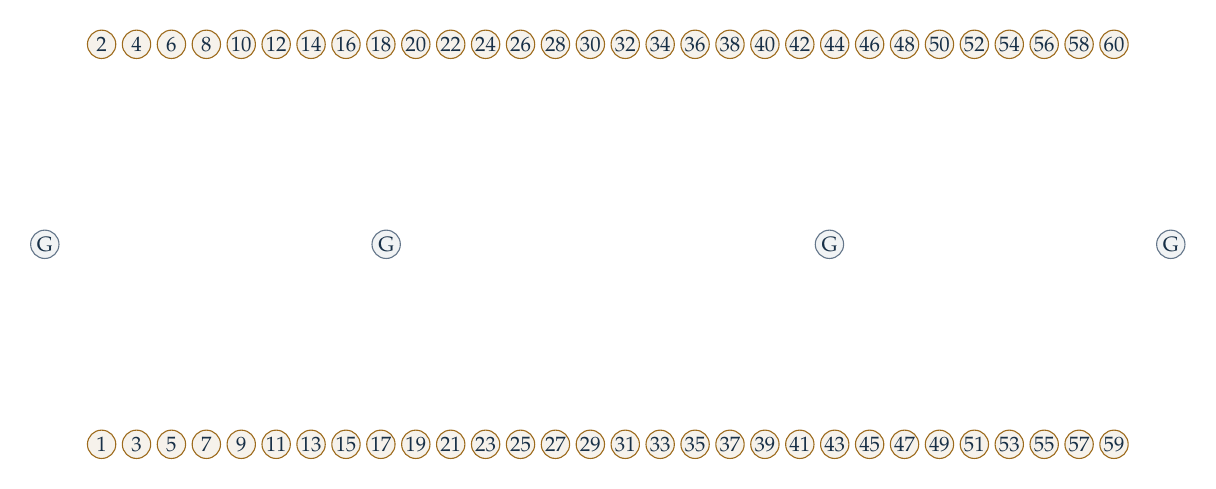
\begin{tikzpicture}[x=1mm,y=-1mm]
\draw[draw=amber,fill=amber!9,line width=.4pt] (7.213,50.799) circle (1.8);
\node[font=\fontsize{7.5}{8}\selectfont,text=navy] at (7.213,50.799) {1};
\draw[draw=amber,fill=amber!9,line width=.4pt] (24.947,0.000) circle (1.8);
\node[font=\fontsize{7.5}{8}\selectfont,text=navy] at (24.947,0.000) {10};
\draw[draw=amber,fill=amber!9,line width=.4pt] (29.381,50.799) circle (1.8);
\node[font=\fontsize{7.5}{8}\selectfont,text=navy] at (29.381,50.799) {11};
\draw[draw=amber,fill=amber!9,line width=.4pt] (29.381,0.000) circle (1.8);
\node[font=\fontsize{7.5}{8}\selectfont,text=navy] at (29.381,0.000) {12};
\draw[draw=amber,fill=amber!9,line width=.4pt] (33.814,50.799) circle (1.8);
\node[font=\fontsize{7.5}{8}\selectfont,text=navy] at (33.814,50.799) {13};
\draw[draw=amber,fill=amber!9,line width=.4pt] (33.814,0.000) circle (1.8);
\node[font=\fontsize{7.5}{8}\selectfont,text=navy] at (33.814,0.000) {14};
\draw[draw=amber,fill=amber!9,line width=.4pt] (38.248,50.799) circle (1.8);
\node[font=\fontsize{7.5}{8}\selectfont,text=navy] at (38.248,50.799) {15};
\draw[draw=amber,fill=amber!9,line width=.4pt] (38.248,0.000) circle (1.8);
\node[font=\fontsize{7.5}{8}\selectfont,text=navy] at (38.248,0.000) {16};
\draw[draw=amber,fill=amber!9,line width=.4pt] (42.681,50.799) circle (1.8);
\node[font=\fontsize{7.5}{8}\selectfont,text=navy] at (42.681,50.799) {17};
\draw[draw=amber,fill=amber!9,line width=.4pt] (42.681,0.000) circle (1.8);
\node[font=\fontsize{7.5}{8}\selectfont,text=navy] at (42.681,0.000) {18};
\draw[draw=amber,fill=amber!9,line width=.4pt] (47.115,50.799) circle (1.8);
\node[font=\fontsize{7.5}{8}\selectfont,text=navy] at (47.115,50.799) {19};
\draw[draw=amber,fill=amber!9,line width=.4pt] (7.213,0.000) circle (1.8);
\node[font=\fontsize{7.5}{8}\selectfont,text=navy] at (7.213,0.000) {2};
\draw[draw=amber,fill=amber!9,line width=.4pt] (47.115,0.000) circle (1.8);
\node[font=\fontsize{7.5}{8}\selectfont,text=navy] at (47.115,0.000) {20};
\draw[draw=amber,fill=amber!9,line width=.4pt] (51.549,50.799) circle (1.8);
\node[font=\fontsize{7.5}{8}\selectfont,text=navy] at (51.549,50.799) {21};
\draw[draw=amber,fill=amber!9,line width=.4pt] (51.549,0.000) circle (1.8);
\node[font=\fontsize{7.5}{8}\selectfont,text=navy] at (51.549,0.000) {22};
\draw[draw=amber,fill=amber!9,line width=.4pt] (55.982,50.799) circle (1.8);
\node[font=\fontsize{7.5}{8}\selectfont,text=navy] at (55.982,50.799) {23};
\draw[draw=amber,fill=amber!9,line width=.4pt] (55.982,0.000) circle (1.8);
\node[font=\fontsize{7.5}{8}\selectfont,text=navy] at (55.982,0.000) {24};
\draw[draw=amber,fill=amber!9,line width=.4pt] (60.416,50.799) circle (1.8);
\node[font=\fontsize{7.5}{8}\selectfont,text=navy] at (60.416,50.799) {25};
\draw[draw=amber,fill=amber!9,line width=.4pt] (60.416,0.000) circle (1.8);
\node[font=\fontsize{7.5}{8}\selectfont,text=navy] at (60.416,0.000) {26};
\draw[draw=amber,fill=amber!9,line width=.4pt] (64.850,50.799) circle (1.8);
\node[font=\fontsize{7.5}{8}\selectfont,text=navy] at (64.850,50.799) {27};
\draw[draw=amber,fill=amber!9,line width=.4pt] (64.850,0.000) circle (1.8);
\node[font=\fontsize{7.5}{8}\selectfont,text=navy] at (64.850,0.000) {28};
\draw[draw=amber,fill=amber!9,line width=.4pt] (69.283,50.799) circle (1.8);
\node[font=\fontsize{7.5}{8}\selectfont,text=navy] at (69.283,50.799) {29};
\draw[draw=amber,fill=amber!9,line width=.4pt] (11.646,50.799) circle (1.8);
\node[font=\fontsize{7.5}{8}\selectfont,text=navy] at (11.646,50.799) {3};
\draw[draw=amber,fill=amber!9,line width=.4pt] (69.283,0.000) circle (1.8);
\node[font=\fontsize{7.5}{8}\selectfont,text=navy] at (69.283,0.000) {30};
\draw[draw=amber,fill=amber!9,line width=.4pt] (73.717,50.799) circle (1.8);
\node[font=\fontsize{7.5}{8}\selectfont,text=navy] at (73.717,50.799) {31};
\draw[draw=amber,fill=amber!9,line width=.4pt] (73.717,0.000) circle (1.8);
\node[font=\fontsize{7.5}{8}\selectfont,text=navy] at (73.717,0.000) {32};
\draw[draw=amber,fill=amber!9,line width=.4pt] (78.150,50.799) circle (1.8);
\node[font=\fontsize{7.5}{8}\selectfont,text=navy] at (78.150,50.799) {33};
\draw[draw=amber,fill=amber!9,line width=.4pt] (78.150,0.000) circle (1.8);
\node[font=\fontsize{7.5}{8}\selectfont,text=navy] at (78.150,0.000) {34};
\draw[draw=amber,fill=amber!9,line width=.4pt] (82.584,50.799) circle (1.8);
\node[font=\fontsize{7.5}{8}\selectfont,text=navy] at (82.584,50.799) {35};
\draw[draw=amber,fill=amber!9,line width=.4pt] (82.584,0.000) circle (1.8);
\node[font=\fontsize{7.5}{8}\selectfont,text=navy] at (82.584,0.000) {36};
\draw[draw=amber,fill=amber!9,line width=.4pt] (87.018,50.799) circle (1.8);
\node[font=\fontsize{7.5}{8}\selectfont,text=navy] at (87.018,50.799) {37};
\draw[draw=amber,fill=amber!9,line width=.4pt] (87.018,0.000) circle (1.8);
\node[font=\fontsize{7.5}{8}\selectfont,text=navy] at (87.018,0.000) {38};
\draw[draw=amber,fill=amber!9,line width=.4pt] (91.451,50.799) circle (1.8);
\node[font=\fontsize{7.5}{8}\selectfont,text=navy] at (91.451,50.799) {39};
\draw[draw=amber,fill=amber!9,line width=.4pt] (11.646,0.000) circle (1.8);
\node[font=\fontsize{7.5}{8}\selectfont,text=navy] at (11.646,0.000) {4};
\draw[draw=amber,fill=amber!9,line width=.4pt] (91.451,0.000) circle (1.8);
\node[font=\fontsize{7.5}{8}\selectfont,text=navy] at (91.451,0.000) {40};
\draw[draw=amber,fill=amber!9,line width=.4pt] (95.885,50.799) circle (1.8);
\node[font=\fontsize{7.5}{8}\selectfont,text=navy] at (95.885,50.799) {41};
\draw[draw=amber,fill=amber!9,line width=.4pt] (95.885,0.000) circle (1.8);
\node[font=\fontsize{7.5}{8}\selectfont,text=navy] at (95.885,0.000) {42};
\draw[draw=amber,fill=amber!9,line width=.4pt] (100.319,50.799) circle (1.8);
\node[font=\fontsize{7.5}{8}\selectfont,text=navy] at (100.319,50.799) {43};
\draw[draw=amber,fill=amber!9,line width=.4pt] (100.319,0.000) circle (1.8);
\node[font=\fontsize{7.5}{8}\selectfont,text=navy] at (100.319,0.000) {44};
\draw[draw=amber,fill=amber!9,line width=.4pt] (104.752,50.799) circle (1.8);
\node[font=\fontsize{7.5}{8}\selectfont,text=navy] at (104.752,50.799) {45};
\draw[draw=amber,fill=amber!9,line width=.4pt] (104.752,0.000) circle (1.8);
\node[font=\fontsize{7.5}{8}\selectfont,text=navy] at (104.752,0.000) {46};
\draw[draw=amber,fill=amber!9,line width=.4pt] (109.186,50.799) circle (1.8);
\node[font=\fontsize{7.5}{8}\selectfont,text=navy] at (109.186,50.799) {47};
\draw[draw=amber,fill=amber!9,line width=.4pt] (109.186,0.000) circle (1.8);
\node[font=\fontsize{7.5}{8}\selectfont,text=navy] at (109.186,0.000) {48};
\draw[draw=amber,fill=amber!9,line width=.4pt] (113.619,50.799) circle (1.8);
\node[font=\fontsize{7.5}{8}\selectfont,text=navy] at (113.619,50.799) {49};
\draw[draw=amber,fill=amber!9,line width=.4pt] (16.080,50.799) circle (1.8);
\node[font=\fontsize{7.5}{8}\selectfont,text=navy] at (16.080,50.799) {5};
\draw[draw=amber,fill=amber!9,line width=.4pt] (113.619,0.000) circle (1.8);
\node[font=\fontsize{7.5}{8}\selectfont,text=navy] at (113.619,0.000) {50};
\draw[draw=amber,fill=amber!9,line width=.4pt] (118.053,50.799) circle (1.8);
\node[font=\fontsize{7.5}{8}\selectfont,text=navy] at (118.053,50.799) {51};
\draw[draw=amber,fill=amber!9,line width=.4pt] (118.053,0.000) circle (1.8);
\node[font=\fontsize{7.5}{8}\selectfont,text=navy] at (118.053,0.000) {52};
\draw[draw=amber,fill=amber!9,line width=.4pt] (122.487,50.799) circle (1.8);
\node[font=\fontsize{7.5}{8}\selectfont,text=navy] at (122.487,50.799) {53};
\draw[draw=amber,fill=amber!9,line width=.4pt] (122.487,0.000) circle (1.8);
\node[font=\fontsize{7.5}{8}\selectfont,text=navy] at (122.487,0.000) {54};
\draw[draw=amber,fill=amber!9,line width=.4pt] (126.920,50.799) circle (1.8);
\node[font=\fontsize{7.5}{8}\selectfont,text=navy] at (126.920,50.799) {55};
\draw[draw=amber,fill=amber!9,line width=.4pt] (126.920,0.000) circle (1.8);
\node[font=\fontsize{7.5}{8}\selectfont,text=navy] at (126.920,0.000) {56};
\draw[draw=amber,fill=amber!9,line width=.4pt] (131.354,50.799) circle (1.8);
\node[font=\fontsize{7.5}{8}\selectfont,text=navy] at (131.354,50.799) {57};
\draw[draw=amber,fill=amber!9,line width=.4pt] (131.354,0.000) circle (1.8);
\node[font=\fontsize{7.5}{8}\selectfont,text=navy] at (131.354,0.000) {58};
\draw[draw=amber,fill=amber!9,line width=.4pt] (135.787,50.799) circle (1.8);
\node[font=\fontsize{7.5}{8}\selectfont,text=navy] at (135.787,50.799) {59};
\draw[draw=amber,fill=amber!9,line width=.4pt] (16.080,0.000) circle (1.8);
\node[font=\fontsize{7.5}{8}\selectfont,text=navy] at (16.080,0.000) {6};
\draw[draw=amber,fill=amber!9,line width=.4pt] (135.787,0.000) circle (1.8);
\node[font=\fontsize{7.5}{8}\selectfont,text=navy] at (135.787,0.000) {60};
\draw[draw=amber,fill=amber!9,line width=.4pt] (20.513,50.799) circle (1.8);
\node[font=\fontsize{7.5}{8}\selectfont,text=navy] at (20.513,50.799) {7};
\draw[draw=amber,fill=amber!9,line width=.4pt] (20.513,0.000) circle (1.8);
\node[font=\fontsize{7.5}{8}\selectfont,text=navy] at (20.513,0.000) {8};
\draw[draw=amber,fill=amber!9,line width=.4pt] (24.947,50.799) circle (1.8);
\node[font=\fontsize{7.5}{8}\selectfont,text=navy] at (24.947,50.799) {9};
\draw[draw=muted,fill=muted!9,line width=.4pt] (0.000,25.400) circle (1.8);
\node[font=\fontsize{7.5}{8}\selectfont,text=navy] at (0.000,25.400) {G};
\draw[draw=muted,fill=muted!9,line width=.4pt] (43.352,25.400) circle (1.8);
\node[font=\fontsize{7.5}{8}\selectfont,text=navy] at (43.352,25.400) {G};
\draw[draw=muted,fill=muted!9,line width=.4pt] (99.648,25.400) circle (1.8);
\node[font=\fontsize{7.5}{8}\selectfont,text=navy] at (99.648,25.400) {G};
\draw[draw=muted,fill=muted!9,line width=.4pt] (143.000,25.400) circle (1.8);
\node[font=\fontsize{7.5}{8}\selectfont,text=navy] at (143.000,25.400) {G};
\end{tikzpicture}\end{center}
\textbf{J6 -- second 60-contact mezzanine}

\begin{center}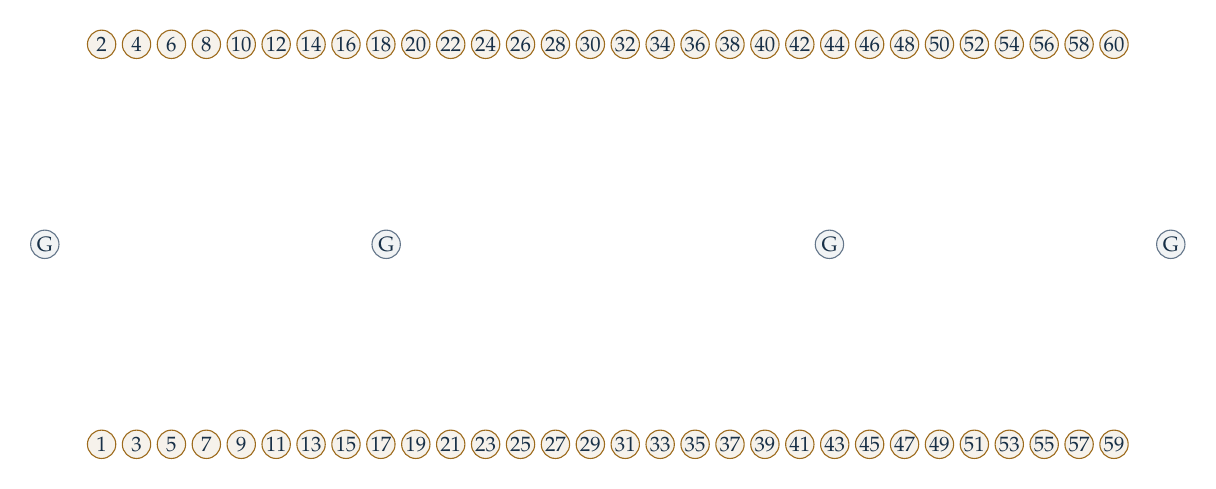
\begin{tikzpicture}[x=1mm,y=-1mm]
\draw[draw=amber,fill=amber!9,line width=.4pt] (7.213,50.799) circle (1.8);
\node[font=\fontsize{7.5}{8}\selectfont,text=navy] at (7.213,50.799) {1};
\draw[draw=amber,fill=amber!9,line width=.4pt] (24.947,0.000) circle (1.8);
\node[font=\fontsize{7.5}{8}\selectfont,text=navy] at (24.947,0.000) {10};
\draw[draw=amber,fill=amber!9,line width=.4pt] (29.381,50.799) circle (1.8);
\node[font=\fontsize{7.5}{8}\selectfont,text=navy] at (29.381,50.799) {11};
\draw[draw=amber,fill=amber!9,line width=.4pt] (29.381,0.000) circle (1.8);
\node[font=\fontsize{7.5}{8}\selectfont,text=navy] at (29.381,0.000) {12};
\draw[draw=amber,fill=amber!9,line width=.4pt] (33.814,50.799) circle (1.8);
\node[font=\fontsize{7.5}{8}\selectfont,text=navy] at (33.814,50.799) {13};
\draw[draw=amber,fill=amber!9,line width=.4pt] (33.814,0.000) circle (1.8);
\node[font=\fontsize{7.5}{8}\selectfont,text=navy] at (33.814,0.000) {14};
\draw[draw=amber,fill=amber!9,line width=.4pt] (38.248,50.799) circle (1.8);
\node[font=\fontsize{7.5}{8}\selectfont,text=navy] at (38.248,50.799) {15};
\draw[draw=amber,fill=amber!9,line width=.4pt] (38.248,0.000) circle (1.8);
\node[font=\fontsize{7.5}{8}\selectfont,text=navy] at (38.248,0.000) {16};
\draw[draw=amber,fill=amber!9,line width=.4pt] (42.681,50.799) circle (1.8);
\node[font=\fontsize{7.5}{8}\selectfont,text=navy] at (42.681,50.799) {17};
\draw[draw=amber,fill=amber!9,line width=.4pt] (42.681,0.000) circle (1.8);
\node[font=\fontsize{7.5}{8}\selectfont,text=navy] at (42.681,0.000) {18};
\draw[draw=amber,fill=amber!9,line width=.4pt] (47.115,50.799) circle (1.8);
\node[font=\fontsize{7.5}{8}\selectfont,text=navy] at (47.115,50.799) {19};
\draw[draw=amber,fill=amber!9,line width=.4pt] (7.213,0.000) circle (1.8);
\node[font=\fontsize{7.5}{8}\selectfont,text=navy] at (7.213,0.000) {2};
\draw[draw=amber,fill=amber!9,line width=.4pt] (47.115,0.000) circle (1.8);
\node[font=\fontsize{7.5}{8}\selectfont,text=navy] at (47.115,0.000) {20};
\draw[draw=amber,fill=amber!9,line width=.4pt] (51.549,50.799) circle (1.8);
\node[font=\fontsize{7.5}{8}\selectfont,text=navy] at (51.549,50.799) {21};
\draw[draw=amber,fill=amber!9,line width=.4pt] (51.549,0.000) circle (1.8);
\node[font=\fontsize{7.5}{8}\selectfont,text=navy] at (51.549,0.000) {22};
\draw[draw=amber,fill=amber!9,line width=.4pt] (55.982,50.799) circle (1.8);
\node[font=\fontsize{7.5}{8}\selectfont,text=navy] at (55.982,50.799) {23};
\draw[draw=amber,fill=amber!9,line width=.4pt] (55.982,0.000) circle (1.8);
\node[font=\fontsize{7.5}{8}\selectfont,text=navy] at (55.982,0.000) {24};
\draw[draw=amber,fill=amber!9,line width=.4pt] (60.416,50.799) circle (1.8);
\node[font=\fontsize{7.5}{8}\selectfont,text=navy] at (60.416,50.799) {25};
\draw[draw=amber,fill=amber!9,line width=.4pt] (60.416,0.000) circle (1.8);
\node[font=\fontsize{7.5}{8}\selectfont,text=navy] at (60.416,0.000) {26};
\draw[draw=amber,fill=amber!9,line width=.4pt] (64.850,50.799) circle (1.8);
\node[font=\fontsize{7.5}{8}\selectfont,text=navy] at (64.850,50.799) {27};
\draw[draw=amber,fill=amber!9,line width=.4pt] (64.850,0.000) circle (1.8);
\node[font=\fontsize{7.5}{8}\selectfont,text=navy] at (64.850,0.000) {28};
\draw[draw=amber,fill=amber!9,line width=.4pt] (69.283,50.799) circle (1.8);
\node[font=\fontsize{7.5}{8}\selectfont,text=navy] at (69.283,50.799) {29};
\draw[draw=amber,fill=amber!9,line width=.4pt] (11.646,50.799) circle (1.8);
\node[font=\fontsize{7.5}{8}\selectfont,text=navy] at (11.646,50.799) {3};
\draw[draw=amber,fill=amber!9,line width=.4pt] (69.283,0.000) circle (1.8);
\node[font=\fontsize{7.5}{8}\selectfont,text=navy] at (69.283,0.000) {30};
\draw[draw=amber,fill=amber!9,line width=.4pt] (73.717,50.799) circle (1.8);
\node[font=\fontsize{7.5}{8}\selectfont,text=navy] at (73.717,50.799) {31};
\draw[draw=amber,fill=amber!9,line width=.4pt] (73.717,0.000) circle (1.8);
\node[font=\fontsize{7.5}{8}\selectfont,text=navy] at (73.717,0.000) {32};
\draw[draw=amber,fill=amber!9,line width=.4pt] (78.150,50.799) circle (1.8);
\node[font=\fontsize{7.5}{8}\selectfont,text=navy] at (78.150,50.799) {33};
\draw[draw=amber,fill=amber!9,line width=.4pt] (78.150,0.000) circle (1.8);
\node[font=\fontsize{7.5}{8}\selectfont,text=navy] at (78.150,0.000) {34};
\draw[draw=amber,fill=amber!9,line width=.4pt] (82.584,50.799) circle (1.8);
\node[font=\fontsize{7.5}{8}\selectfont,text=navy] at (82.584,50.799) {35};
\draw[draw=amber,fill=amber!9,line width=.4pt] (82.584,0.000) circle (1.8);
\node[font=\fontsize{7.5}{8}\selectfont,text=navy] at (82.584,0.000) {36};
\draw[draw=amber,fill=amber!9,line width=.4pt] (87.018,50.799) circle (1.8);
\node[font=\fontsize{7.5}{8}\selectfont,text=navy] at (87.018,50.799) {37};
\draw[draw=amber,fill=amber!9,line width=.4pt] (87.018,0.000) circle (1.8);
\node[font=\fontsize{7.5}{8}\selectfont,text=navy] at (87.018,0.000) {38};
\draw[draw=amber,fill=amber!9,line width=.4pt] (91.451,50.799) circle (1.8);
\node[font=\fontsize{7.5}{8}\selectfont,text=navy] at (91.451,50.799) {39};
\draw[draw=amber,fill=amber!9,line width=.4pt] (11.646,0.000) circle (1.8);
\node[font=\fontsize{7.5}{8}\selectfont,text=navy] at (11.646,0.000) {4};
\draw[draw=amber,fill=amber!9,line width=.4pt] (91.451,0.000) circle (1.8);
\node[font=\fontsize{7.5}{8}\selectfont,text=navy] at (91.451,0.000) {40};
\draw[draw=amber,fill=amber!9,line width=.4pt] (95.885,50.799) circle (1.8);
\node[font=\fontsize{7.5}{8}\selectfont,text=navy] at (95.885,50.799) {41};
\draw[draw=amber,fill=amber!9,line width=.4pt] (95.885,0.000) circle (1.8);
\node[font=\fontsize{7.5}{8}\selectfont,text=navy] at (95.885,0.000) {42};
\draw[draw=amber,fill=amber!9,line width=.4pt] (100.319,50.799) circle (1.8);
\node[font=\fontsize{7.5}{8}\selectfont,text=navy] at (100.319,50.799) {43};
\draw[draw=amber,fill=amber!9,line width=.4pt] (100.319,0.000) circle (1.8);
\node[font=\fontsize{7.5}{8}\selectfont,text=navy] at (100.319,0.000) {44};
\draw[draw=amber,fill=amber!9,line width=.4pt] (104.752,50.799) circle (1.8);
\node[font=\fontsize{7.5}{8}\selectfont,text=navy] at (104.752,50.799) {45};
\draw[draw=amber,fill=amber!9,line width=.4pt] (104.752,0.000) circle (1.8);
\node[font=\fontsize{7.5}{8}\selectfont,text=navy] at (104.752,0.000) {46};
\draw[draw=amber,fill=amber!9,line width=.4pt] (109.186,50.799) circle (1.8);
\node[font=\fontsize{7.5}{8}\selectfont,text=navy] at (109.186,50.799) {47};
\draw[draw=amber,fill=amber!9,line width=.4pt] (109.186,0.000) circle (1.8);
\node[font=\fontsize{7.5}{8}\selectfont,text=navy] at (109.186,0.000) {48};
\draw[draw=amber,fill=amber!9,line width=.4pt] (113.619,50.799) circle (1.8);
\node[font=\fontsize{7.5}{8}\selectfont,text=navy] at (113.619,50.799) {49};
\draw[draw=amber,fill=amber!9,line width=.4pt] (16.080,50.799) circle (1.8);
\node[font=\fontsize{7.5}{8}\selectfont,text=navy] at (16.080,50.799) {5};
\draw[draw=amber,fill=amber!9,line width=.4pt] (113.619,0.000) circle (1.8);
\node[font=\fontsize{7.5}{8}\selectfont,text=navy] at (113.619,0.000) {50};
\draw[draw=amber,fill=amber!9,line width=.4pt] (118.053,50.799) circle (1.8);
\node[font=\fontsize{7.5}{8}\selectfont,text=navy] at (118.053,50.799) {51};
\draw[draw=amber,fill=amber!9,line width=.4pt] (118.053,0.000) circle (1.8);
\node[font=\fontsize{7.5}{8}\selectfont,text=navy] at (118.053,0.000) {52};
\draw[draw=amber,fill=amber!9,line width=.4pt] (122.487,50.799) circle (1.8);
\node[font=\fontsize{7.5}{8}\selectfont,text=navy] at (122.487,50.799) {53};
\draw[draw=amber,fill=amber!9,line width=.4pt] (122.487,0.000) circle (1.8);
\node[font=\fontsize{7.5}{8}\selectfont,text=navy] at (122.487,0.000) {54};
\draw[draw=amber,fill=amber!9,line width=.4pt] (126.920,50.799) circle (1.8);
\node[font=\fontsize{7.5}{8}\selectfont,text=navy] at (126.920,50.799) {55};
\draw[draw=amber,fill=amber!9,line width=.4pt] (126.920,0.000) circle (1.8);
\node[font=\fontsize{7.5}{8}\selectfont,text=navy] at (126.920,0.000) {56};
\draw[draw=amber,fill=amber!9,line width=.4pt] (131.354,50.799) circle (1.8);
\node[font=\fontsize{7.5}{8}\selectfont,text=navy] at (131.354,50.799) {57};
\draw[draw=amber,fill=amber!9,line width=.4pt] (131.354,0.000) circle (1.8);
\node[font=\fontsize{7.5}{8}\selectfont,text=navy] at (131.354,0.000) {58};
\draw[draw=amber,fill=amber!9,line width=.4pt] (135.787,50.799) circle (1.8);
\node[font=\fontsize{7.5}{8}\selectfont,text=navy] at (135.787,50.799) {59};
\draw[draw=amber,fill=amber!9,line width=.4pt] (16.080,0.000) circle (1.8);
\node[font=\fontsize{7.5}{8}\selectfont,text=navy] at (16.080,0.000) {6};
\draw[draw=amber,fill=amber!9,line width=.4pt] (135.787,0.000) circle (1.8);
\node[font=\fontsize{7.5}{8}\selectfont,text=navy] at (135.787,0.000) {60};
\draw[draw=amber,fill=amber!9,line width=.4pt] (20.513,50.799) circle (1.8);
\node[font=\fontsize{7.5}{8}\selectfont,text=navy] at (20.513,50.799) {7};
\draw[draw=amber,fill=amber!9,line width=.4pt] (20.513,0.000) circle (1.8);
\node[font=\fontsize{7.5}{8}\selectfont,text=navy] at (20.513,0.000) {8};
\draw[draw=amber,fill=amber!9,line width=.4pt] (24.947,50.799) circle (1.8);
\node[font=\fontsize{7.5}{8}\selectfont,text=navy] at (24.947,50.799) {9};
\draw[draw=muted,fill=muted!9,line width=.4pt] (0.000,25.400) circle (1.8);
\node[font=\fontsize{7.5}{8}\selectfont,text=navy] at (0.000,25.400) {G};
\draw[draw=muted,fill=muted!9,line width=.4pt] (43.352,25.400) circle (1.8);
\node[font=\fontsize{7.5}{8}\selectfont,text=navy] at (43.352,25.400) {G};
\draw[draw=muted,fill=muted!9,line width=.4pt] (99.648,25.400) circle (1.8);
\node[font=\fontsize{7.5}{8}\selectfont,text=navy] at (99.648,25.400) {G};
\draw[draw=muted,fill=muted!9,line width=.4pt] (143.000,25.400) circle (1.8);
\node[font=\fontsize{7.5}{8}\selectfont,text=navy] at (143.000,25.400) {G};
\end{tikzpicture}\end{center}
{\small All 120 numbered J5/J6 contacts are amber: unassigned. Each set of G lands shares one electrical G endpoint. The shared GND net still has gaps.}

\textbf{Before a mating board can be released:} reconcile connector top/bottom views, connector orientation and the final contact-to-FPGA map on both sides. A clear drawing does not by itself establish that the two boards will mate electrically.

\textbf{How to read the rows.} The saved orientation places even-numbered contacts in the upper row and odd-numbered contacts in the lower row. The layout of the mating connector may be viewed from the opposite side; confirm the manufacturer's drawing rather than copying this picture as a mating-face map.


\clearpage\section{J4: read the custom cable contact map}\label{sec:cablemap}

J4 uses the shape of a micro-HDMI connector with a custom electrical assignment. View the map from the PCB front, as for J5/J6. Repeated SH labels are shell pads on one electrical endpoint. Amber contacts are unassigned, gray contacts belong to nets with gaps, and teal contacts are on fully connected assigned nets.

\begin{center}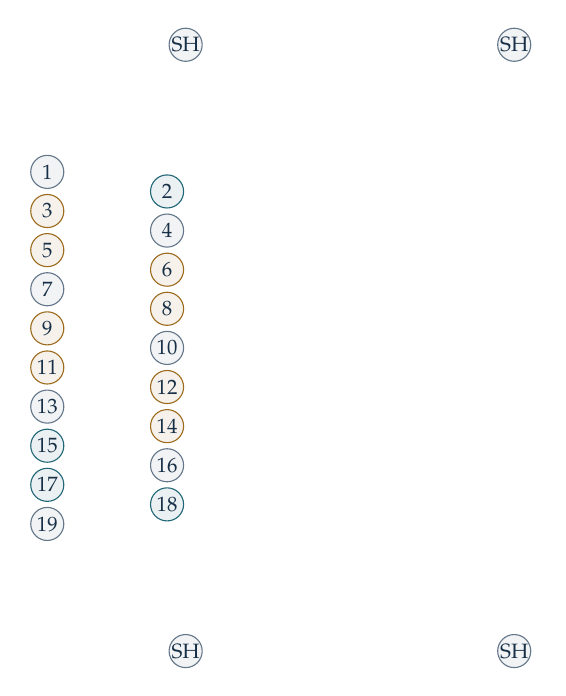
\begin{tikzpicture}[x=1mm,y=-1mm]
\draw[draw=muted,fill=muted!9,line width=.4pt] (0.000,16.145) circle (2.1);
\node[font=\fontsize{7.5}{8}\selectfont,text=navy] at (0.000,16.145) {1};
\draw[draw=muted,fill=muted!9,line width=.4pt] (15.214,38.500) circle (2.1);
\node[font=\fontsize{7.5}{8}\selectfont,text=navy] at (15.214,38.500) {10};
\draw[draw=amber,fill=amber!9,line width=.4pt] (0.000,40.984) circle (2.1);
\node[font=\fontsize{7.5}{8}\selectfont,text=navy] at (0.000,40.984) {11};
\draw[draw=amber,fill=amber!9,line width=.4pt] (15.214,43.468) circle (2.1);
\node[font=\fontsize{7.5}{8}\selectfont,text=navy] at (15.214,43.468) {12};
\draw[draw=muted,fill=muted!9,line width=.4pt] (0.000,45.952) circle (2.1);
\node[font=\fontsize{7.5}{8}\selectfont,text=navy] at (0.000,45.952) {13};
\draw[draw=amber,fill=amber!9,line width=.4pt] (15.214,48.435) circle (2.1);
\node[font=\fontsize{7.5}{8}\selectfont,text=navy] at (15.214,48.435) {14};
\draw[draw=teal,fill=teal!9,line width=.4pt] (0.000,50.919) circle (2.1);
\node[font=\fontsize{7.5}{8}\selectfont,text=navy] at (0.000,50.919) {15};
\draw[draw=muted,fill=muted!9,line width=.4pt] (15.214,53.403) circle (2.1);
\node[font=\fontsize{7.5}{8}\selectfont,text=navy] at (15.214,53.403) {16};
\draw[draw=teal,fill=teal!9,line width=.4pt] (0.000,55.887) circle (2.1);
\node[font=\fontsize{7.5}{8}\selectfont,text=navy] at (0.000,55.887) {17};
\draw[draw=teal,fill=teal!9,line width=.4pt] (15.214,58.371) circle (2.1);
\node[font=\fontsize{7.5}{8}\selectfont,text=navy] at (15.214,58.371) {18};
\draw[draw=muted,fill=muted!9,line width=.4pt] (0.000,60.855) circle (2.1);
\node[font=\fontsize{7.5}{8}\selectfont,text=navy] at (0.000,60.855) {19};
\draw[draw=teal,fill=teal!9,line width=.4pt] (15.214,18.629) circle (2.1);
\node[font=\fontsize{7.5}{8}\selectfont,text=navy] at (15.214,18.629) {2};
\draw[draw=amber,fill=amber!9,line width=.4pt] (0.000,21.113) circle (2.1);
\node[font=\fontsize{7.5}{8}\selectfont,text=navy] at (0.000,21.113) {3};
\draw[draw=muted,fill=muted!9,line width=.4pt] (15.214,23.597) circle (2.1);
\node[font=\fontsize{7.5}{8}\selectfont,text=navy] at (15.214,23.597) {4};
\draw[draw=amber,fill=amber!9,line width=.4pt] (0.000,26.081) circle (2.1);
\node[font=\fontsize{7.5}{8}\selectfont,text=navy] at (0.000,26.081) {5};
\draw[draw=amber,fill=amber!9,line width=.4pt] (15.214,28.565) circle (2.1);
\node[font=\fontsize{7.5}{8}\selectfont,text=navy] at (15.214,28.565) {6};
\draw[draw=muted,fill=muted!9,line width=.4pt] (0.000,31.048) circle (2.1);
\node[font=\fontsize{7.5}{8}\selectfont,text=navy] at (0.000,31.048) {7};
\draw[draw=amber,fill=amber!9,line width=.4pt] (15.214,33.532) circle (2.1);
\node[font=\fontsize{7.5}{8}\selectfont,text=navy] at (15.214,33.532) {8};
\draw[draw=amber,fill=amber!9,line width=.4pt] (0.000,36.016) circle (2.1);
\node[font=\fontsize{7.5}{8}\selectfont,text=navy] at (0.000,36.016) {9};
\draw[draw=muted,fill=muted!9,line width=.4pt] (17.573,77.000) circle (2.1);
\node[font=\fontsize{7.5}{8}\selectfont,text=navy] at (17.573,77.000) {SH};
\draw[draw=muted,fill=muted!9,line width=.4pt] (59.302,77.000) circle (2.1);
\node[font=\fontsize{7.5}{8}\selectfont,text=navy] at (59.302,77.000) {SH};
\draw[draw=muted,fill=muted!9,line width=.4pt] (17.573,0.000) circle (2.1);
\node[font=\fontsize{7.5}{8}\selectfont,text=navy] at (17.573,0.000) {SH};
\draw[draw=muted,fill=muted!9,line width=.4pt] (59.302,0.000) circle (2.1);
\node[font=\fontsize{7.5}{8}\selectfont,text=navy] at (59.302,0.000) {SH};
\end{tikzpicture}\end{center}
\textbf{The saved assignments, one contact at a time}

\begingroup\fontsize{9.2}{11.7}\selectfont\setlength{\tabcolsep}{2.8pt}\renewcommand{\arraystretch}{0.92}
\begin{longtable}{@{}P{34mm}P{113mm}P{15mm}@{}}
\toprule \textbf{Endpoint} & \textbf{Saved net / state} & \textbf{Code} \\ \midrule
\endfirsthead\toprule \textbf{Endpoint} & \textbf{Saved net / state} & \textbf{Code} \\ \midrule
\endhead\midrule\multicolumn{3}{r}{\footnotesize Continued on next page}\endfoot\bottomrule\endlastfoot
\nolinkurl{J4.1} & \nolinkurl{VCCAUX_1V8} & P \\
\nolinkurl{J4.2} & \nolinkurl{JTAG_TMS} & C \\
\nolinkurl{J4.3} & Unassigned & U \\
\nolinkurl{J4.4} & \nolinkurl{GND} & P \\
\nolinkurl{J4.5} & Unassigned & U \\
\nolinkurl{J4.6} & Unassigned & U \\
\nolinkurl{J4.7} & \nolinkurl{GND} & P \\
\nolinkurl{J4.8} & Unassigned & U \\
\nolinkurl{J4.9} & Unassigned & U \\
\nolinkurl{J4.10} & \nolinkurl{GND} & P \\
\nolinkurl{J4.11} & Unassigned & U \\
\nolinkurl{J4.12} & Unassigned & U \\
\nolinkurl{J4.13} & \nolinkurl{GND} & P \\
\nolinkurl{J4.14} & Unassigned & U \\
\nolinkurl{J4.15} & \nolinkurl{JTAG_TDI} & C \\
\nolinkurl{J4.16} & \nolinkurl{GND} & P \\
\nolinkurl{J4.17} & \nolinkurl{JTAG_TCK} & C \\
\nolinkurl{J4.18} & \nolinkurl{JTAG_TDO} & C \\
\nolinkurl{J4.19} & \nolinkurl{LINK_12V} & P \\
\nolinkurl{J4.SH} & \nolinkurl{GND} & P \\
\end{longtable}\endgroup

\textbf{Read an example.} J4.17 is JTAG TCK; J4.19 is the proposed 12 V input. J4.3 and J4.5 are an unassigned lane-pair position. The eight lane contacts are not connected to FPGA balls yet. Ground returns, cable orientation, carrier mapping and electrical limits still need verification. Do not connect standard HDMI equipment.


\clearpage\section{Which components can we reconsider?}\label{sec:minimum}

The review asks two separate questions: \textbf{is the function needed?} and \textbf{is this exact implementation the smallest adequate one?} A part can support a necessary function while its value, quantity or footprint remains open to optimization.

\begingroup\fontsize{9.8}{12.3}\selectfont\setlength{\tabcolsep}{2.8pt}\renewcommand{\arraystretch}{1.12}
\begin{longtable}{@{}P{53mm}P{13mm}P{100mm}@{}}
\toprule \textbf{Decision class} & \textbf{Parts} & \textbf{Interpretation} \\ \midrule
\endfirsthead\toprule \textbf{Decision class} & \textbf{Parts} & \textbf{Interpretation} \\ \midrule
\endhead\midrule\multicolumn{3}{r}{\footnotesize Continued on next page}\endfoot\bottomrule\endlastfoot
Keep function & 32 & Essential in this topology; an equivalent redesign is possible. \\
Depends on system choice & 13 & Needed by the chosen boot, clock, rail or connection strategy. \\
Check before reducing & 84 & Supports power, startup or signal quality; exact individual minimum is unproven. \\
Removal candidate & 1 & R12: its present status signal has no functional consumer. \\
\end{longtable}\endgroup

\begingroup\fontsize{9.1}{11.6}\selectfont\setlength{\tabcolsep}{2.8pt}\renewcommand{\arraystretch}{1.12}
\begin{longtable}{@{}P{40mm}P{57mm}P{69mm}@{}}
\toprule \textbf{Candidate / group} & \textbf{Reason} & \textbf{Required action before claiming success} \\ \midrule
\endfirsthead\toprule \textbf{Candidate / group} & \textbf{Reason} & \textbf{Required action before claiming success} \\ \midrule
\endhead\midrule\multicolumn{3}{r}{\footnotesize Continued on next page}\endfoot\bottomrule\endlastfoot
R12 & PGOOD\_IO has no consumer. & Remove/review its branch deliberately, or give it a monitoring function. \\
R110 & DONE already has an internal pull-up. & Check startup configuration and loading before removing the external pull-up. \\
R111-R114 & Mode/PUDC\_B straps can use fixed ties. & Preserve the intended logic states in the redesigned copper. \\
R104 / R106 / R107 & Fitted zero-ohm signal links. & Replace by reviewed copper; an empty footprint would break the signal. \\
Capacitors and damping parts & Network performance matters more than count. & Demonstrate supply/edge behavior with the actual load, routing and assembly. \\
J4 / J5 / J6 & Each serves the chosen system interface. & No separate J2/J3 debug header or test-point component remains to remove. \\
\end{longtable}\endgroup

\textbf{Why not shrink the outline immediately?} The 15 $\times$ 15 mm FPGA is only one object in a 33 $\times$ 36 mm board. Remaining space may be required for BGA escape, rail distribution, ground returns, connector access and assembly tolerance. The present minimum courtyard gap of about 0.010 mm is not an assembler-approved clearance. J4's drawn body adds about 0.65 mm beyond one edge.

The board is the \textbf{smallest published checkpoint}, not a demonstrated global minimum or a qualified complete assembly. There is no proof that reducing the count by one part reduces the outline.

\saybox{We have one clear removal candidate and several conditional simplifications. We should optimize the circuit and routing against measurable requirements, not infer that every empty patch of the drawing is wasted area.}


\clearpage\section{What has been checked, and what has not?}\label{sec:checks}

\textbf{DRC} checks PCB geometry against the saved design rules. \textbf{ERC} checks schematic electrical-rule categories. \textbf{Parity} checks correspondence between the saved schematic and PCB. These are useful checks, but a wrong connection can be copied consistently into both files.

\begingroup\fontsize{9.3}{11.8}\selectfont\setlength{\tabcolsep}{2.8pt}\renewcommand{\arraystretch}{1.12}
\begin{longtable}{@{}P{41mm}P{37mm}P{88mm}@{}}
\toprule \textbf{Check} & \textbf{Saved result} & \textbf{Meaning / limitation} \\ \midrule
\endfirsthead\toprule \textbf{Check} & \textbf{Saved result} & \textbf{Meaning / limitation} \\ \midrule
\endhead\midrule\multicolumn{3}{r}{\footnotesize Continued on next page}\endfoot\bottomrule\endlastfoot
Components / endpoints & 130 / 762 & Explained and cross-checked against saved evidence. \\
Physical DRC / parity & 0 / 0 & No reported geometry/parity findings under the saved rules; not electrical approval. \\
Assigned-net connectivity & 146 gaps & Power/ground routing remains; this count excludes unassigned interfaces. \\
Unassigned endpoints & 331 & 203 FPGA + 120 mezzanine + eight cable contacts. \\
Schematic ERC & 331 open pins + 5 warnings & Known open interfaces and symbol-type warnings remain. \\
Boot / clock / JTAG nets & 25 nets connected & Copper connectivity; no demonstrated programming or cold boot. \\
Power-good nets & 2 sequencing + 1 status & The status net is unconsumed; it is not a third enable stage. \\
Built hardware & Not tested & No rail, thermal, capture or sustained-link measurements from this board. \\
\end{longtable}\endgroup

\textbf{Where the 146 gaps are recorded}

\begingroup\fontsize{9.2}{11.7}\selectfont\setlength{\tabcolsep}{2.8pt}\renewcommand{\arraystretch}{1.12}
\begin{longtable}{@{}P{64mm}P{15mm}P{64mm}P{15mm}@{}}
\toprule \textbf{Net} & \textbf{Gaps} & \textbf{Net} & \textbf{Gaps} \\ \midrule
\endfirsthead\toprule \textbf{Net} & \textbf{Gaps} & \textbf{Net} & \textbf{Gaps} \\ \midrule
\endhead\midrule\multicolumn{4}{r}{\footnotesize Continued on next page}\endfoot\bottomrule\endlastfoot
\nolinkurl{GND} & 8 & \nolinkurl{LINK_12V} & 9 \\
\nolinkurl{VAUX_REG_1V803} & 1 & \nolinkurl{VCCAUX_1V8} & 49 \\
\nolinkurl{VCCINT_1V0} & 34 & \nolinkurl{VCC_ASIC_1V5} & 37 \\
\nolinkurl{VCC_LINK_2V5} & 8 & Total & 146 \\
\end{longtable}\endgroup

\textbf{U4.11 is a useful example.} Its schematic net is GND, but its VSEL copper strap is still open. Pin 3 is the converter's high-current GND terminal; the two pin functions should not be confused. The U1 diode-pin error is different again: those pins need a corrected net assignment, so it is not included in the 146 assigned-net count.

\saybox{The saved layout passes its geometry and parity checks. That does not make the circuitry correct or complete: we still have power routing, interface assignments, electrical corrections and hardware tests ahead.}


\clearpage\section{A briefing you can give to your professor}\label{sec:briefing}

\saybox{Our smallest published PCB is 33 by 36 millimeters and uses a 100T FPGA in a 15 by 15 millimeter package. It is intended to capture the eight-ASIC interface and send data to the XEM8310 receiver. Its 130 components fall into seven functions: FPGA logic, power, decoupling, boot memory, clock, startup/programming and three connectors.}

\textbf{Continue with the design choices.}\par
``The four local supplies support the core, auxiliary/configuration circuits and two interface-voltage domains. J5 and J6 are the requested two 60-contact mezzanines. J4 combines custom cable power and JTAG, with data contacts still to assign. There are no separate debug headers, user LEDs or standalone test points in this version.''

\textbf{Then state the honest result.}\par
``The component audit found that R12 has no current consumer. Other reductions require specific circuit or performance checks. We also found two FPGA pins that must be grounded and four regulator pins needing grounding review. These findings are documented, but the native circuit is unchanged. The design still has 146 assigned-net gaps and 331 unassigned endpoints.''

\textbf{Questions to be ready for}

\begingroup\fontsize{9.3}{11.8}\selectfont\setlength{\tabcolsep}{2.8pt}\renewcommand{\arraystretch}{1.12}
\begin{longtable}{@{}P{56mm}P{112mm}@{}}
\toprule \textbf{Question} & \textbf{Answer} \\ \midrule
\endfirsthead\toprule \textbf{Question} & \textbf{Answer} \\ \midrule
\endhead\midrule\multicolumn{2}{r}{\footnotesize Continued on next page}\endfoot\bottomrule\endlastfoot
Is every capacitor mandatory? & The network function is necessary. We have not demonstrated that every individual capacitor is the minimum adequate population. \\
Why use flash? & It enables autonomous configuration after power-up. Removing it requires another configuration source. \\
Are 203 FPGA pins spare? & No. They are unassigned today; the application and link maps have not been implemented. \\
Does zero DRC mean it works? & No. It checks saved geometry rules. Electrical requirements and powered behavior are separate. \\
Can 120 contacts carry 117 signals? & The count fits with three proposed reserves plus separate ground lands. Mapping, electrical and timing validation remain. \\
What is the next evidence needed? & Approved ASIC pad/timing data; closed pin/cable contracts; corrected schematic; complete qualified routing; then prototype measurements. \\
\end{longtable}\endgroup

\textbf{Use the report during questions.} Find a part in Appendix~\ref{app:parts}; find a ball or contact in Appendices~\ref{app:fpga}--\ref{app:devices}. A P label means the net has a gap somewhere, while G/R explicitly identifies a pending connection correction or review.


\clearpage\section{Sources, revision and reading limits}\label{sec:sources}

This is a learning report derived from the current saved circuit and the later component/unused-pin audit. It supersedes the earlier report's interpretation of the six NC markers; it does not modify native CAD or claim fabrication readiness. Manufacturer statements and the actual saved net assignments are kept separate from engineering choices that still need validation.

\textbf{Native board SHA-256}\par

\nolinkurl{ae601df3925e5ec5e90c8a2e747356e432d0558e820199cf7c01c6bf8a7fef96}


\textbf{Source records.} The report uses the current component list, all-pin CSV, native readback, routing snapshot, component necessity audit and pin-status dataset. The portable source archive includes these ledgers and a coverage record. All 130 components and 762 endpoint IDs are covered; the appendices contain each endpoint once in their primary tables.

\textbf{Primary references and project evidence}
\begingroup\small\begin{enumerate}[label={[\arabic*]},leftmargin=8mm,itemsep=4pt]
\item \href{https://www.ti.com/lit/ds/symlink/tps62135.pdf}{Texas Instruments, TPS62135/TPS621351 datasheet.} Pin table p3; single-divider circuit Figure 5 p16; distributed capacitance pp32--33; layout p36. FB2 grounding remains a review finding, not an implemented correction.
\item \href{https://docs.amd.com/api/khub/documents/iAkxxTOk96ANLJqYf2hgrQ/content}{AMD DS181, Artix-7 DC and AC characteristics.} Supply limits, sequencing and ramp requirements.
\item \href{https://docs.amd.com/api/khub/documents/6L8DUUei7ZCE78qwQafC3A/content}{AMD UG483, 7 Series PCB Design Guide.} Capacitor guidance, placement and power-network analysis.
\item \href{https://docs.amd.com/v/u/en-US/ug470_7Series_Config}{AMD UG470, 7 Series Configuration User Guide.} Configuration voltages, mode/PUDC\_B straps, PROGRAM\_B/INIT\_B pull-ups and DONE behavior.
\item \href{https://www.macronix.com/Lists/Datasheet/Attachments/8704/MX25U12835F,\%201.8V,\%20128Mb,\%20v1.9.pdf}{Macronix MX25U12835F, 1.8 V flash, v1.9.} Exact-part pin 7 is RESET/SIO3.
\item \href{https://abracon.com/Oscillators/ASE3series.pdf}{Abracon ASE3 series oscillator datasheet.} Supply and four-pin mapping. A generic bypass note has mismatched 7/14-pin wording; the selected four-pin table is used here.
\item \href{https://docs.amd.com/api/khub/documents/kHyYQ6XzXnQwR2O~gaV~MQ/content}{AMD UG475 v1.20, Table 1-12, p26.} Unused DXP/DXN pins require GND. This is the basis for the two explicit corrections.
\item \href{https://howardwhsrun.github.io/FPGA_4K/sources/slides/Chip_FPGA_Interface.pdf}{Gerald's ASIC interface slides, pp14--17 and 25--28.} Recording/SPI tutorial behavior. Timing/channel-label conflicts and missing electrical limits are preserved as open questions. The team's later correction adds four SPI clocks to reach 117 signals.
\item \href{https://docs.opalkelly.com/xem8310/}{Opal Kelly XEM8310 documentation.} Downstream FPGA module and interface context; no automatic target-power or JTAG bridge is assumed.
\item \href{https://github.com/controlpaths/cp_som_one/tree/b272899d62ac2e454f85c413d64d62271137da27}{Controlpaths CP SOM ONE, pinned reference revision.} Power/schematic/layout reference; its device, package and load differ from this board.
\end{enumerate}\endgroup

\textbf{Status boundary.} No new ERC/DRC or powered hardware test was performed for this document. The numerical CAD results refer to the frozen source board. The later manufacturer review adds the diode-ground and FB2 findings. Routing, ASIC/XEM8310 electrical contracts, firmware, timing, power integrity, thermal and manufacturing approval remain unfinished.

\clearpage\appendix\section{Every component: purpose and removal consequence}\label{app:parts}
Use this as a lookup table. The decision categories apply to the current topology, not to every possible FPGA design. K = keep function; S = system choice; Q = qualify before reduction; X = removal candidate. Values are saved design values, not a released procurement list.

Every two-terminal part lists both actual endpoints. Larger devices point to the complete tables that follow. C/P/U/G/R are pin/net status codes from page~\pageref{sec:pinstatus}; G/R replace any implication that a saved NC marker is approved final wiring.

\begingroup\fontsize{8.7}{11.2}\selectfont\setlength{\tabcolsep}{2.8pt}\renewcommand{\arraystretch}{1.05}
\begin{longtable}{@{}P{27mm}P{77mm}P{62mm}@{}}
\toprule \textbf{Part / value} & \textbf{Role; consequence if removed} & \textbf{Actual endpoint: net [status]} \\ \midrule
\endfirsthead\toprule \textbf{Part / value} & \textbf{Role; consequence if removed} & \textbf{Actual endpoint: net [status]} \\ \midrule
\endhead\midrule\multicolumn{3}{r}{\footnotesize Continued on next page}\endfoot\bottomrule\endlastfoot
\textbf{C1} [Q]\newline 47u 25V X5R & \textbf{Cable-entry bulk reservoir}\newline Reduces cable-entry energy reserve; depends on cable impedance, inrush and source behavior. & \nolinkurl{C1.1}: \nolinkurl{LINK_12V} [P]\newline \nolinkurl{C1.2}: \nolinkurl{GND} [P] \\
\textbf{C2} [Q]\newline 100n 100V X7R & \textbf{Cable-entry high-frequency bypass}\newline Changes entry-node high-frequency impedance. & \nolinkurl{C2.1}: \nolinkurl{LINK_12V} [P]\newline \nolinkurl{C2.2}: \nolinkurl{GND} [P] \\
\textbf{C3} [K]\newline 22u 25V X5R & \textbf{Converter input reservoir}\newline The local current loop relies on distant capacitors and cable inductance; input ripple and unstable startup become possible. & \nolinkurl{C3.1}: \nolinkurl{LINK_12V} [P]\newline \nolinkurl{C3.2}: \nolinkurl{GND} [P] \\
\textbf{C4} [Q]\newline 100n 100V X7R & \textbf{High-frequency input bypass}\newline Changes high-frequency input impedance. The larger capacitor may not behave identically at fast edges. & \nolinkurl{C4.1}: \nolinkurl{LINK_12V} [P]\newline \nolinkurl{C4.2}: \nolinkurl{GND} [P] \\
\textbf{C5} [K]\newline 22u 16V X5R & \textbf{Converter local output capacitor}\newline The output filter and sensed node lose their intended local capacitor; supply ripple and control behavior change. & \nolinkurl{C5.1}: \nolinkurl{VCORE_REG_1V025} [C]\newline \nolinkurl{C5.2}: \nolinkurl{GND} [P] \\
\textbf{C6} [Q]\newline 10n 50V X7R & \textbf{Soft-start timing capacitor}\newline The converter uses its fast internal startup behavior; inrush and FPGA rail ramp/sequence change. & \nolinkurl{C6.1}: \nolinkurl{SS_CORE} [C]\newline \nolinkurl{C6.2}: \nolinkurl{GND} [P] \\
\textbf{C7} [K]\newline 22u 25V X5R & \textbf{Converter input reservoir}\newline The local current loop relies on distant capacitors and cable inductance; input ripple and unstable startup become possible. & \nolinkurl{C7.1}: \nolinkurl{LINK_12V} [P]\newline \nolinkurl{C7.2}: \nolinkurl{GND} [P] \\
\textbf{C8} [Q]\newline 100n 100V X7R & \textbf{High-frequency input bypass}\newline Changes high-frequency input impedance. The larger capacitor may not behave identically at fast edges. & \nolinkurl{C8.1}: \nolinkurl{LINK_12V} [P]\newline \nolinkurl{C8.2}: \nolinkurl{GND} [P] \\
\textbf{C9} [K]\newline 22u 16V X5R & \textbf{Converter local output capacitor}\newline The output filter and sensed node lose their intended local capacitor; supply ripple and control behavior change. & \nolinkurl{C9.1}: \nolinkurl{VAUX_REG_1V803} [P]\newline \nolinkurl{C9.2}: \nolinkurl{GND} [P] \\
\textbf{C10} [Q]\newline 10n 50V X7R & \textbf{Soft-start timing capacitor}\newline The converter uses its fast internal startup behavior; inrush and FPGA rail ramp/sequence change. & \nolinkurl{C10.1}: \nolinkurl{SS_AUX} [C]\newline \nolinkurl{C10.2}: \nolinkurl{GND} [P] \\
\textbf{C11} [K]\newline 22u 25V X5R & \textbf{Converter input reservoir}\newline The local current loop relies on distant capacitors and cable inductance; input ripple and unstable startup become possible. & \nolinkurl{C11.1}: \nolinkurl{LINK_12V} [P]\newline \nolinkurl{C11.2}: \nolinkurl{GND} [P] \\
\textbf{C12} [Q]\newline 100n 100V X7R & \textbf{High-frequency input bypass}\newline Changes high-frequency input impedance. The larger capacitor may not behave identically at fast edges. & \nolinkurl{C12.1}: \nolinkurl{LINK_12V} [P]\newline \nolinkurl{C12.2}: \nolinkurl{GND} [P] \\
\textbf{C13} [K]\newline 22u 16V X5R & \textbf{Converter local output capacitor}\newline The output filter and sensed node lose their intended local capacitor; supply ripple and control behavior change. & \nolinkurl{C13.1}: \nolinkurl{VCC_LINK_2V5} [P]\newline \nolinkurl{C13.2}: \nolinkurl{GND} [P] \\
\textbf{C14} [Q]\newline 10n 50V X7R & \textbf{Soft-start timing capacitor}\newline The converter uses its fast internal startup behavior; inrush and FPGA rail ramp/sequence change. & \nolinkurl{C14.1}: \nolinkurl{SS_CFG} [C]\newline \nolinkurl{C14.2}: \nolinkurl{GND} [P] \\
\textbf{C15} [K]\newline 22u 25V X5R & \textbf{Converter input reservoir}\newline The local current loop relies on distant capacitors and cable inductance; input ripple and unstable startup become possible. & \nolinkurl{C15.1}: \nolinkurl{LINK_12V} [P]\newline \nolinkurl{C15.2}: \nolinkurl{GND} [P] \\
\textbf{C16} [Q]\newline 100n 100V X7R & \textbf{High-frequency input bypass}\newline Changes high-frequency input impedance. The larger capacitor may not behave identically at fast edges. & \nolinkurl{C16.1}: \nolinkurl{LINK_12V} [P]\newline \nolinkurl{C16.2}: \nolinkurl{GND} [P] \\
\textbf{C17} [K]\newline 22u 16V X5R & \textbf{Converter local output capacitor}\newline The output filter and sensed node lose their intended local capacitor; supply ripple and control behavior change. & \nolinkurl{C17.1}: \nolinkurl{VCC_ASIC_1V5} [P]\newline \nolinkurl{C17.2}: \nolinkurl{GND} [P] \\
\textbf{C18} [Q]\newline 10n 50V X7R & \textbf{Soft-start timing capacitor}\newline The converter uses its fast internal startup behavior; inrush and FPGA rail ramp/sequence change. & \nolinkurl{C18.1}: \nolinkurl{SS_ASIC} [C]\newline \nolinkurl{C18.2}: \nolinkurl{GND} [P] \\
\textbf{C20} [Q]\newline 330u 2.5V polymer ESR25m & \textbf{Bulk energy reserve}\newline Less local stored charge and changed power-network impedance; may cause supply noise or transient failures. Removing one is not automatically safe or automatically fatal. & \nolinkurl{C20.1}: \nolinkurl{VCCINT_1V0} [P]\newline \nolinkurl{C20.2}: \nolinkurl{GND} [P] \\
\textbf{C21} [Q]\newline 100u 6.3V X5R & \textbf{Bulk energy reserve}\newline Less local stored charge and changed power-network impedance; may cause supply noise or transient failures. Removing one is not automatically safe or automatically fatal. & \nolinkurl{C21.1}: \nolinkurl{VCCINT_1V0} [P]\newline \nolinkurl{C21.2}: \nolinkurl{GND} [P] \\
\textbf{C22} [Q]\newline 4.7u 10V X7R & \textbf{Local supply bypass}\newline Less local stored charge and changed power-network impedance; may cause supply noise or transient failures. Removing one is not automatically safe or automatically fatal. & \nolinkurl{C22.1}: \nolinkurl{VCCINT_1V0} [P]\newline \nolinkurl{C22.2}: \nolinkurl{GND} [P] \\
\textbf{C23} [Q]\newline 4.7u 10V X7R & \textbf{Local supply bypass}\newline Less local stored charge and changed power-network impedance; may cause supply noise or transient failures. Removing one is not automatically safe or automatically fatal. & \nolinkurl{C23.1}: \nolinkurl{VCCINT_1V0} [P]\newline \nolinkurl{C23.2}: \nolinkurl{GND} [P] \\
\textbf{C24} [Q]\newline 4.7u 10V X7R & \textbf{Local supply bypass}\newline Less local stored charge and changed power-network impedance; may cause supply noise or transient failures. Removing one is not automatically safe or automatically fatal. & \nolinkurl{C24.1}: \nolinkurl{VCCINT_1V0} [P]\newline \nolinkurl{C24.2}: \nolinkurl{GND} [P] \\
\textbf{C25} [Q]\newline 4.7u 10V X7R & \textbf{Local supply bypass}\newline Less local stored charge and changed power-network impedance; may cause supply noise or transient failures. Removing one is not automatically safe or automatically fatal. & \nolinkurl{C25.1}: \nolinkurl{VCCINT_1V0} [P]\newline \nolinkurl{C25.2}: \nolinkurl{GND} [P] \\
\textbf{C26} [Q]\newline 4.7u 10V X7R & \textbf{Local supply bypass}\newline Less local stored charge and changed power-network impedance; may cause supply noise or transient failures. Removing one is not automatically safe or automatically fatal. & \nolinkurl{C26.1}: \nolinkurl{VCCINT_1V0} [P]\newline \nolinkurl{C26.2}: \nolinkurl{GND} [P] \\
\textbf{C27} [Q]\newline 4.7u 10V X7R & \textbf{Local supply bypass}\newline Less local stored charge and changed power-network impedance; may cause supply noise or transient failures. Removing one is not automatically safe or automatically fatal. & \nolinkurl{C27.1}: \nolinkurl{VCCINT_1V0} [P]\newline \nolinkurl{C27.2}: \nolinkurl{GND} [P] \\
\textbf{C28} [Q]\newline 470n 6.3V X7R & \textbf{Local supply bypass}\newline Less local stored charge and changed power-network impedance; may cause supply noise or transient failures. Removing one is not automatically safe or automatically fatal. & \nolinkurl{C28.1}: \nolinkurl{VCCINT_1V0} [P]\newline \nolinkurl{C28.2}: \nolinkurl{GND} [P] \\
\textbf{C29} [Q]\newline 470n 6.3V X7R & \textbf{Local supply bypass}\newline Less local stored charge and changed power-network impedance; may cause supply noise or transient failures. Removing one is not automatically safe or automatically fatal. & \nolinkurl{C29.1}: \nolinkurl{VCCINT_1V0} [P]\newline \nolinkurl{C29.2}: \nolinkurl{GND} [P] \\
\textbf{C30} [Q]\newline 470n 6.3V X7R & \textbf{Local supply bypass}\newline Less local stored charge and changed power-network impedance; may cause supply noise or transient failures. Removing one is not automatically safe or automatically fatal. & \nolinkurl{C30.1}: \nolinkurl{VCCINT_1V0} [P]\newline \nolinkurl{C30.2}: \nolinkurl{GND} [P] \\
\textbf{C31} [Q]\newline 470n 6.3V X7R & \textbf{Local supply bypass}\newline Less local stored charge and changed power-network impedance; may cause supply noise or transient failures. Removing one is not automatically safe or automatically fatal. & \nolinkurl{C31.1}: \nolinkurl{VCCINT_1V0} [P]\newline \nolinkurl{C31.2}: \nolinkurl{GND} [P] \\
\textbf{C32} [Q]\newline 470n 6.3V X7R & \textbf{Local supply bypass}\newline Less local stored charge and changed power-network impedance; may cause supply noise or transient failures. Removing one is not automatically safe or automatically fatal. & \nolinkurl{C32.1}: \nolinkurl{VCCINT_1V0} [P]\newline \nolinkurl{C32.2}: \nolinkurl{GND} [P] \\
\textbf{C33} [Q]\newline 470n 6.3V X7R & \textbf{Local supply bypass}\newline Less local stored charge and changed power-network impedance; may cause supply noise or transient failures. Removing one is not automatically safe or automatically fatal. & \nolinkurl{C33.1}: \nolinkurl{VCCINT_1V0} [P]\newline \nolinkurl{C33.2}: \nolinkurl{GND} [P] \\
\textbf{C34} [Q]\newline 470n 6.3V X7R & \textbf{Local supply bypass}\newline Less local stored charge and changed power-network impedance; may cause supply noise or transient failures. Removing one is not automatically safe or automatically fatal. & \nolinkurl{C34.1}: \nolinkurl{VCCINT_1V0} [P]\newline \nolinkurl{C34.2}: \nolinkurl{GND} [P] \\
\textbf{C35} [Q]\newline 470n 6.3V X7R & \textbf{Local supply bypass}\newline Less local stored charge and changed power-network impedance; may cause supply noise or transient failures. Removing one is not automatically safe or automatically fatal. & \nolinkurl{C35.1}: \nolinkurl{VCCINT_1V0} [P]\newline \nolinkurl{C35.2}: \nolinkurl{GND} [P] \\
\textbf{C36} [Q]\newline 470n 6.3V X7R & \textbf{Local supply bypass}\newline Less local stored charge and changed power-network impedance; may cause supply noise or transient failures. Removing one is not automatically safe or automatically fatal. & \nolinkurl{C36.1}: \nolinkurl{VCCINT_1V0} [P]\newline \nolinkurl{C36.2}: \nolinkurl{GND} [P] \\
\textbf{C37} [Q]\newline 470n 6.3V X7R & \textbf{Local supply bypass}\newline Less local stored charge and changed power-network impedance; may cause supply noise or transient failures. Removing one is not automatically safe or automatically fatal. & \nolinkurl{C37.1}: \nolinkurl{VCCINT_1V0} [P]\newline \nolinkurl{C37.2}: \nolinkurl{GND} [P] \\
\textbf{C40} [Q]\newline 47u 6.3V X7R & \textbf{Bulk energy reserve}\newline Less local stored charge and changed power-network impedance; may cause supply noise or transient failures. Removing one is not automatically safe or automatically fatal. & \nolinkurl{C40.1}: \nolinkurl{VCCAUX_1V8} [P]\newline \nolinkurl{C40.2}: \nolinkurl{GND} [P] \\
\textbf{C41} [Q]\newline 4.7u 10V X7R & \textbf{Local supply bypass}\newline Less local stored charge and changed power-network impedance; may cause supply noise or transient failures. Removing one is not automatically safe or automatically fatal. & \nolinkurl{C41.1}: \nolinkurl{VCCAUX_1V8} [P]\newline \nolinkurl{C41.2}: \nolinkurl{GND} [P] \\
\textbf{C42} [Q]\newline 4.7u 10V X7R & \textbf{Local supply bypass}\newline Less local stored charge and changed power-network impedance; may cause supply noise or transient failures. Removing one is not automatically safe or automatically fatal. & \nolinkurl{C42.1}: \nolinkurl{VCCAUX_1V8} [P]\newline \nolinkurl{C42.2}: \nolinkurl{GND} [P] \\
\textbf{C43} [Q]\newline 470n 6.3V X7R & \textbf{Local supply bypass}\newline Less local stored charge and changed power-network impedance; may cause supply noise or transient failures. Removing one is not automatically safe or automatically fatal. & \nolinkurl{C43.1}: \nolinkurl{VCCAUX_1V8} [P]\newline \nolinkurl{C43.2}: \nolinkurl{GND} [P] \\
\textbf{C44} [Q]\newline 470n 6.3V X7R & \textbf{Local supply bypass}\newline Less local stored charge and changed power-network impedance; may cause supply noise or transient failures. Removing one is not automatically safe or automatically fatal. & \nolinkurl{C44.1}: \nolinkurl{VCCAUX_1V8} [P]\newline \nolinkurl{C44.2}: \nolinkurl{GND} [P] \\
\textbf{C45} [Q]\newline 470n 6.3V X7R & \textbf{Local supply bypass}\newline Less local stored charge and changed power-network impedance; may cause supply noise or transient failures. Removing one is not automatically safe or automatically fatal. & \nolinkurl{C45.1}: \nolinkurl{VCCAUX_1V8} [P]\newline \nolinkurl{C45.2}: \nolinkurl{GND} [P] \\
\textbf{C46} [Q]\newline 470n 6.3V X7R & \textbf{Local supply bypass}\newline Less local stored charge and changed power-network impedance; may cause supply noise or transient failures. Removing one is not automatically safe or automatically fatal. & \nolinkurl{C46.1}: \nolinkurl{VCCAUX_1V8} [P]\newline \nolinkurl{C46.2}: \nolinkurl{GND} [P] \\
\textbf{C50} [Q]\newline 47u 6.3V X7R & \textbf{Bulk energy reserve}\newline Less local stored charge and changed power-network impedance; may cause supply noise or transient failures. Removing one is not automatically safe or automatically fatal. & \nolinkurl{C50.1}: \nolinkurl{VCCAUX_1V8} [P]\newline \nolinkurl{C50.2}: \nolinkurl{GND} [P] \\
\textbf{C51} [Q]\newline 4.7u 10V X7R & \textbf{Local supply bypass}\newline Less local stored charge and changed power-network impedance; may cause supply noise or transient failures. Removing one is not automatically safe or automatically fatal. & \nolinkurl{C51.1}: \nolinkurl{VCCAUX_1V8} [P]\newline \nolinkurl{C51.2}: \nolinkurl{GND} [P] \\
\textbf{C52} [Q]\newline 4.7u 10V X7R & \textbf{Local supply bypass}\newline Less local stored charge and changed power-network impedance; may cause supply noise or transient failures. Removing one is not automatically safe or automatically fatal. & \nolinkurl{C52.1}: \nolinkurl{VCCAUX_1V8} [P]\newline \nolinkurl{C52.2}: \nolinkurl{GND} [P] \\
\textbf{C53} [Q]\newline 470n 6.3V X7R & \textbf{Local supply bypass}\newline Less local stored charge and changed power-network impedance; may cause supply noise or transient failures. Removing one is not automatically safe or automatically fatal. & \nolinkurl{C53.1}: \nolinkurl{VCCAUX_1V8} [P]\newline \nolinkurl{C53.2}: \nolinkurl{GND} [P] \\
\textbf{C54} [Q]\newline 470n 6.3V X7R & \textbf{Local supply bypass}\newline Less local stored charge and changed power-network impedance; may cause supply noise or transient failures. Removing one is not automatically safe or automatically fatal. & \nolinkurl{C54.1}: \nolinkurl{VCCAUX_1V8} [P]\newline \nolinkurl{C54.2}: \nolinkurl{GND} [P] \\
\textbf{C55} [Q]\newline 470n 6.3V X7R & \textbf{Local supply bypass}\newline Less local stored charge and changed power-network impedance; may cause supply noise or transient failures. Removing one is not automatically safe or automatically fatal. & \nolinkurl{C55.1}: \nolinkurl{VCCAUX_1V8} [P]\newline \nolinkurl{C55.2}: \nolinkurl{GND} [P] \\
\textbf{C56} [Q]\newline 470n 6.3V X7R & \textbf{Local supply bypass}\newline Less local stored charge and changed power-network impedance; may cause supply noise or transient failures. Removing one is not automatically safe or automatically fatal. & \nolinkurl{C56.1}: \nolinkurl{VCCAUX_1V8} [P]\newline \nolinkurl{C56.2}: \nolinkurl{GND} [P] \\
\textbf{C57} [Q]\newline 4.7u 10V X7R & \textbf{Local supply bypass}\newline Less local stored charge and changed power-network impedance; may cause supply noise or transient failures. Removing one is not automatically safe or automatically fatal. & \nolinkurl{C57.1}: \nolinkurl{VCC_LINK_2V5} [P]\newline \nolinkurl{C57.2}: \nolinkurl{GND} [P] \\
\textbf{C58} [Q]\newline 4.7u 10V X7R & \textbf{Local supply bypass}\newline Less local stored charge and changed power-network impedance; may cause supply noise or transient failures. Removing one is not automatically safe or automatically fatal. & \nolinkurl{C58.1}: \nolinkurl{VCC_LINK_2V5} [P]\newline \nolinkurl{C58.2}: \nolinkurl{GND} [P] \\
\textbf{C59} [Q]\newline 470n 6.3V X7R & \textbf{Local supply bypass}\newline Less local stored charge and changed power-network impedance; may cause supply noise or transient failures. Removing one is not automatically safe or automatically fatal. & \nolinkurl{C59.1}: \nolinkurl{VCC_LINK_2V5} [P]\newline \nolinkurl{C59.2}: \nolinkurl{GND} [P] \\
\textbf{C60} [Q]\newline 470n 6.3V X7R & \textbf{Local supply bypass}\newline Less local stored charge and changed power-network impedance; may cause supply noise or transient failures. Removing one is not automatically safe or automatically fatal. & \nolinkurl{C60.1}: \nolinkurl{VCC_LINK_2V5} [P]\newline \nolinkurl{C60.2}: \nolinkurl{GND} [P] \\
\textbf{C61} [Q]\newline 470n 6.3V X7R & \textbf{Local supply bypass}\newline Less local stored charge and changed power-network impedance; may cause supply noise or transient failures. Removing one is not automatically safe or automatically fatal. & \nolinkurl{C61.1}: \nolinkurl{VCC_LINK_2V5} [P]\newline \nolinkurl{C61.2}: \nolinkurl{GND} [P] \\
\textbf{C62} [Q]\newline 470n 6.3V X7R & \textbf{Local supply bypass}\newline Less local stored charge and changed power-network impedance; may cause supply noise or transient failures. Removing one is not automatically safe or automatically fatal. & \nolinkurl{C62.1}: \nolinkurl{VCC_LINK_2V5} [P]\newline \nolinkurl{C62.2}: \nolinkurl{GND} [P] \\
\textbf{C63} [Q]\newline 47u 6.3V X7R & \textbf{Bulk energy reserve}\newline Less local stored charge and changed power-network impedance; may cause supply noise or transient failures. Removing one is not automatically safe or automatically fatal. & \nolinkurl{C63.1}: \nolinkurl{VCC_LINK_2V5} [P]\newline \nolinkurl{C63.2}: \nolinkurl{GND} [P] \\
\textbf{C64} [Q]\newline 4.7u 10V X7R & \textbf{Local supply bypass}\newline Less local stored charge and changed power-network impedance; may cause supply noise or transient failures. Removing one is not automatically safe or automatically fatal. & \nolinkurl{C64.1}: \nolinkurl{VCC_ASIC_1V5} [P]\newline \nolinkurl{C64.2}: \nolinkurl{GND} [P] \\
\textbf{C65} [Q]\newline 4.7u 10V X7R & \textbf{Local supply bypass}\newline Less local stored charge and changed power-network impedance; may cause supply noise or transient failures. Removing one is not automatically safe or automatically fatal. & \nolinkurl{C65.1}: \nolinkurl{VCC_ASIC_1V5} [P]\newline \nolinkurl{C65.2}: \nolinkurl{GND} [P] \\
\textbf{C66} [Q]\newline 470n 6.3V X7R & \textbf{Local supply bypass}\newline Less local stored charge and changed power-network impedance; may cause supply noise or transient failures. Removing one is not automatically safe or automatically fatal. & \nolinkurl{C66.1}: \nolinkurl{VCC_ASIC_1V5} [P]\newline \nolinkurl{C66.2}: \nolinkurl{GND} [P] \\
\textbf{C67} [Q]\newline 470n 6.3V X7R & \textbf{Local supply bypass}\newline Less local stored charge and changed power-network impedance; may cause supply noise or transient failures. Removing one is not automatically safe or automatically fatal. & \nolinkurl{C67.1}: \nolinkurl{VCC_ASIC_1V5} [P]\newline \nolinkurl{C67.2}: \nolinkurl{GND} [P] \\
\textbf{C68} [Q]\newline 470n 6.3V X7R & \textbf{Local supply bypass}\newline Less local stored charge and changed power-network impedance; may cause supply noise or transient failures. Removing one is not automatically safe or automatically fatal. & \nolinkurl{C68.1}: \nolinkurl{VCC_ASIC_1V5} [P]\newline \nolinkurl{C68.2}: \nolinkurl{GND} [P] \\
\textbf{C69} [Q]\newline 470n 6.3V X7R & \textbf{Local supply bypass}\newline Less local stored charge and changed power-network impedance; may cause supply noise or transient failures. Removing one is not automatically safe or automatically fatal. & \nolinkurl{C69.1}: \nolinkurl{VCC_ASIC_1V5} [P]\newline \nolinkurl{C69.2}: \nolinkurl{GND} [P] \\
\textbf{C70} [Q]\newline 4.7u 10V X7R & \textbf{Local supply bypass}\newline Less local stored charge and changed power-network impedance; may cause supply noise or transient failures. Removing one is not automatically safe or automatically fatal. & \nolinkurl{C70.1}: \nolinkurl{VCC_ASIC_1V5} [P]\newline \nolinkurl{C70.2}: \nolinkurl{GND} [P] \\
\textbf{C71} [Q]\newline 4.7u 10V X7R & \textbf{Local supply bypass}\newline Less local stored charge and changed power-network impedance; may cause supply noise or transient failures. Removing one is not automatically safe or automatically fatal. & \nolinkurl{C71.1}: \nolinkurl{VCC_ASIC_1V5} [P]\newline \nolinkurl{C71.2}: \nolinkurl{GND} [P] \\
\textbf{C72} [Q]\newline 470n 6.3V X7R & \textbf{Local supply bypass}\newline Less local stored charge and changed power-network impedance; may cause supply noise or transient failures. Removing one is not automatically safe or automatically fatal. & \nolinkurl{C72.1}: \nolinkurl{VCC_ASIC_1V5} [P]\newline \nolinkurl{C72.2}: \nolinkurl{GND} [P] \\
\textbf{C73} [Q]\newline 470n 6.3V X7R & \textbf{Local supply bypass}\newline Less local stored charge and changed power-network impedance; may cause supply noise or transient failures. Removing one is not automatically safe or automatically fatal. & \nolinkurl{C73.1}: \nolinkurl{VCC_ASIC_1V5} [P]\newline \nolinkurl{C73.2}: \nolinkurl{GND} [P] \\
\textbf{C74} [Q]\newline 470n 6.3V X7R & \textbf{Local supply bypass}\newline Less local stored charge and changed power-network impedance; may cause supply noise or transient failures. Removing one is not automatically safe or automatically fatal. & \nolinkurl{C74.1}: \nolinkurl{VCC_ASIC_1V5} [P]\newline \nolinkurl{C74.2}: \nolinkurl{GND} [P] \\
\textbf{C75} [Q]\newline 470n 6.3V X7R & \textbf{Local supply bypass}\newline Less local stored charge and changed power-network impedance; may cause supply noise or transient failures. Removing one is not automatically safe or automatically fatal. & \nolinkurl{C75.1}: \nolinkurl{VCC_ASIC_1V5} [P]\newline \nolinkurl{C75.2}: \nolinkurl{GND} [P] \\
\textbf{C76} [Q]\newline 4.7u 10V X7R & \textbf{Local supply bypass}\newline Less local stored charge and changed power-network impedance; may cause supply noise or transient failures. Removing one is not automatically safe or automatically fatal. & \nolinkurl{C76.1}: \nolinkurl{VCC_ASIC_1V5} [P]\newline \nolinkurl{C76.2}: \nolinkurl{GND} [P] \\
\textbf{C77} [Q]\newline 4.7u 10V X7R & \textbf{Local supply bypass}\newline Less local stored charge and changed power-network impedance; may cause supply noise or transient failures. Removing one is not automatically safe or automatically fatal. & \nolinkurl{C77.1}: \nolinkurl{VCC_ASIC_1V5} [P]\newline \nolinkurl{C77.2}: \nolinkurl{GND} [P] \\
\textbf{C78} [Q]\newline 470n 6.3V X7R & \textbf{Local supply bypass}\newline Less local stored charge and changed power-network impedance; may cause supply noise or transient failures. Removing one is not automatically safe or automatically fatal. & \nolinkurl{C78.1}: \nolinkurl{VCC_ASIC_1V5} [P]\newline \nolinkurl{C78.2}: \nolinkurl{GND} [P] \\
\textbf{C79} [Q]\newline 470n 6.3V X7R & \textbf{Local supply bypass}\newline Less local stored charge and changed power-network impedance; may cause supply noise or transient failures. Removing one is not automatically safe or automatically fatal. & \nolinkurl{C79.1}: \nolinkurl{VCC_ASIC_1V5} [P]\newline \nolinkurl{C79.2}: \nolinkurl{GND} [P] \\
\textbf{C80} [Q]\newline 470n 6.3V X7R & \textbf{Local supply bypass}\newline Less local stored charge and changed power-network impedance; may cause supply noise or transient failures. Removing one is not automatically safe or automatically fatal. & \nolinkurl{C80.1}: \nolinkurl{VCC_ASIC_1V5} [P]\newline \nolinkurl{C80.2}: \nolinkurl{GND} [P] \\
\textbf{C81} [Q]\newline 470n 6.3V X7R & \textbf{Local supply bypass}\newline Less local stored charge and changed power-network impedance; may cause supply noise or transient failures. Removing one is not automatically safe or automatically fatal. & \nolinkurl{C81.1}: \nolinkurl{VCC_ASIC_1V5} [P]\newline \nolinkurl{C81.2}: \nolinkurl{GND} [P] \\
\textbf{C82} [Q]\newline 47u 6.3V X7R & \textbf{Bulk energy reserve}\newline Less local stored charge and changed power-network impedance; may cause supply noise or transient failures. Removing one is not automatically safe or automatically fatal. & \nolinkurl{C82.1}: \nolinkurl{VCC_ASIC_1V5} [P]\newline \nolinkurl{C82.2}: \nolinkurl{GND} [P] \\
\textbf{C90} [Q]\newline 100n 16V X7R & \textbf{Local supply bypass}\newline Less local stored charge and changed power-network impedance; may cause supply noise or transient failures. Removing one is not automatically safe or automatically fatal. & \nolinkurl{C90.1}: \nolinkurl{VCCAUX_1V8} [P]\newline \nolinkurl{C90.2}: \nolinkurl{GND} [P] \\
\textbf{C91} [Q]\newline 1u 10V X7R & \textbf{Local supply bypass}\newline Less local stored charge and changed power-network impedance; may cause supply noise or transient failures. Removing one is not automatically safe or automatically fatal. & \nolinkurl{C91.1}: \nolinkurl{VCCAUX_1V8} [P]\newline \nolinkurl{C91.2}: \nolinkurl{GND} [P] \\
\textbf{C92} [Q]\newline 47u 6.3V X7R & \textbf{Bulk energy reserve}\newline Less local stored charge and changed power-network impedance; may cause supply noise or transient failures. Removing one is not automatically safe or automatically fatal. & \nolinkurl{C92.1}: \nolinkurl{VCCAUX_1V8} [P]\newline \nolinkurl{C92.2}: \nolinkurl{GND} [P] \\
\textbf{C100} [K]\newline 100n & \textbf{Flash local supply bypass}\newline Removes the smallest local flash reservoir; remote rail capacitance does not guarantee an equivalent short current loop. & \nolinkurl{C100.1}: \nolinkurl{VCCAUX_1V8} [P]\newline \nolinkurl{C100.2}: \nolinkurl{GND} [P] \\
\textbf{C101} [Q]\newline 1u & \textbf{Flash local bulk reservoir}\newline Less local reserve; flash current transients must then be met by C100 and the rail network. & \nolinkurl{C101.1}: \nolinkurl{VCCAUX_1V8} [P]\newline \nolinkurl{C101.2}: \nolinkurl{GND} [P] \\
\textbf{C102} [K]\newline 10n & \textbf{Oscillator local supply bypass}\newline Removes its intended shortest bypass path. & \nolinkurl{C102.1}: \nolinkurl{VCCAUX_1V8} [P]\newline \nolinkurl{C102.2}: \nolinkurl{GND} [P] \\
\textbf{C103} [Q]\newline 100n & \textbf{Additional oscillator bypass}\newline Less local supply filtering; consequence depends on supply impedance and clock sensitivity. & \nolinkurl{C103.1}: \nolinkurl{VCCAUX_1V8} [P]\newline \nolinkurl{C103.2}: \nolinkurl{GND} [P] \\
\textbf{J4} [S]\newline CUSTOM POWER + JTAG / DATA TBD & \textbf{Shared power / JTAG / future data cable}\newline The selected power-entry and external programming access disappear. & Complete pins: Appendix~\ref{app:connectors}. \\
\textbf{J5} [S]\newline QSH-030-01-L-D-A & \textbf{60-contact ASIC mezzanine}\newline The proposed 117-contact interface no longer fits in the remaining 60 contacts. & Complete pins: Appendix~\ref{app:connectors}. \\
\textbf{J6} [S]\newline QSH-030-01-L-D-A & \textbf{60-contact ASIC mezzanine}\newline The proposed 117-contact interface no longer fits in the remaining 60 contacts. & Complete pins: Appendix~\ref{app:connectors}. \\
\textbf{L1} [K]\newline 1uH 5.4A Isat30\% & \textbf{Buck energy-storage inductor}\newline Open circuit cuts power to the rail; replacing with a short exposes the load to switching pulses. & \nolinkurl{L1.1}: \nolinkurl{SW_CORE} [C]\newline \nolinkurl{L1.2}: \nolinkurl{VCORE_REG_1V025} [C] \\
\textbf{L2} [K]\newline 1uH 5.4A Isat30\% & \textbf{Buck energy-storage inductor}\newline Open circuit cuts power to the rail; replacing with a short exposes the load to switching pulses. & \nolinkurl{L2.1}: \nolinkurl{SW_AUX} [C]\newline \nolinkurl{L2.2}: \nolinkurl{VAUX_REG_1V803} [P] \\
\textbf{L3} [K]\newline 1uH 5.4A Isat30\% & \textbf{Buck energy-storage inductor}\newline Open circuit cuts power to the rail; replacing with a short exposes the load to switching pulses. & \nolinkurl{L3.1}: \nolinkurl{SW_CFG} [C]\newline \nolinkurl{L3.2}: \nolinkurl{VCC_LINK_2V5} [P] \\
\textbf{L4} [K]\newline 1uH 5.4A Isat30\% & \textbf{Buck energy-storage inductor}\newline Open circuit cuts power to the rail; replacing with a short exposes the load to switching pulses. & \nolinkurl{L4.1}: \nolinkurl{SW_ASIC} [C]\newline \nolinkurl{L4.2}: \nolinkurl{VCC_ASIC_1V5} [P] \\
\textbf{R1} [K]\newline 32.4k 0.1\% & \textbf{Core / block ram feedback divider}\newline The intended feedback ratio is lost; the rail may be wrong, too low or driven high. & \nolinkurl{R1.1}: \nolinkurl{VCORE_REG_1V025} [C]\newline \nolinkurl{R1.2}: \nolinkurl{FB_CORE} [C] \\
\textbf{R2} [K]\newline 69.8k 0.1\% & \textbf{Core / block ram feedback divider}\newline The intended feedback ratio is lost; the rail may be wrong, too low or driven high. & \nolinkurl{R2.1}: \nolinkurl{FB_CORE} [C]\newline \nolinkurl{R2.2}: \nolinkurl{GND} [P] \\
\textbf{R3} [K]\newline 110k 0.1\% & \textbf{Auxiliary / configuration feedback divider}\newline The intended feedback ratio is lost; the rail may be wrong, too low or driven high. & \nolinkurl{R3.1}: \nolinkurl{VAUX_REG_1V803} [P]\newline \nolinkurl{R3.2}: \nolinkurl{FB_AUX} [C] \\
\textbf{R4} [K]\newline 69.8k 0.1\% & \textbf{Auxiliary / configuration feedback divider}\newline The intended feedback ratio is lost; the rail may be wrong, too low or driven high. & \nolinkurl{R4.1}: \nolinkurl{FB_AUX} [C]\newline \nolinkurl{R4.2}: \nolinkurl{GND} [P] \\
\textbf{R5} [K]\newline 180k 0.1\% & \textbf{2.5 v link bank feedback divider}\newline The intended feedback ratio is lost; the rail may be wrong, too low or driven high. & \nolinkurl{R5.1}: \nolinkurl{VCC_LINK_2V5} [P]\newline \nolinkurl{R5.2}: \nolinkurl{FB_CFG} [C] \\
\textbf{R6} [K]\newline 69.8k 0.1\% & \textbf{2.5 v link bank feedback divider}\newline The intended feedback ratio is lost; the rail may be wrong, too low or driven high. & \nolinkurl{R6.1}: \nolinkurl{FB_CFG} [C]\newline \nolinkurl{R6.2}: \nolinkurl{GND} [P] \\
\textbf{R7} [K]\newline 80.6k 0.1\% & \textbf{1.5 v asic-facing banks feedback divider}\newline The intended feedback ratio is lost; the rail may be wrong, too low or driven high. & \nolinkurl{R7.1}: \nolinkurl{VCC_ASIC_1V5} [P]\newline \nolinkurl{R7.2}: \nolinkurl{FB_ASIC} [C] \\
\textbf{R8} [K]\newline 69.8k 0.1\% & \textbf{1.5 v asic-facing banks feedback divider}\newline The intended feedback ratio is lost; the rail may be wrong, too low or driven high. & \nolinkurl{R8.1}: \nolinkurl{FB_ASIC} [C]\newline \nolinkurl{R8.2}: \nolinkurl{GND} [P] \\
\textbf{R9} [K]\newline 15m 1\% 1W & \textbf{Distributed-capacitance isolation}\newline Removing it opens the rail; shorting it defeats the deliberately separated local and distributed capacitor networks. & \nolinkurl{R9.1}: \nolinkurl{VCORE_REG_1V025} [C]\newline \nolinkurl{R9.2}: \nolinkurl{VCCINT_1V0} [P] \\
\textbf{R10} [K]\newline 100k & \textbf{Power-up sequencing pull-up}\newline The downstream enable no longer receives its designed high level. & \nolinkurl{R10.1}: \nolinkurl{LINK_12V} [P]\newline \nolinkurl{R10.2}: \nolinkurl{PG_CORE} [C] \\
\textbf{R11} [K]\newline 100k & \textbf{Power-up sequencing pull-up}\newline The downstream enable no longer receives its designed high level. & \nolinkurl{R11.1}: \nolinkurl{LINK_12V} [P]\newline \nolinkurl{R11.2}: \nolinkurl{PG_AUX} [C] \\
\textbf{R12} [X]\newline 100k & \textbf{Unconsumed I/O-good status pull-up}\newline No existing rail-enable or data path is removed. The status branch would lose its defined high state. & \nolinkurl{R12.1}: \nolinkurl{VCCAUX_1V8} [P]\newline \nolinkurl{R12.2}: \nolinkurl{PGOOD_IO} [C] \\
\textbf{R100} [K]\newline 2.4k & \textbf{Flash chip-select pull-up}\newline Flash chip select loses its external defined idle-high state during startup. & \nolinkurl{R100.1}: \nolinkurl{VCCAUX_1V8} [P]\newline \nolinkurl{R100.2}: \nolinkurl{FLASH_CS_B} [C] \\
\textbf{R101} [S]\newline 4.7k & \textbf{Flash WP / DQ2 default high}\newline The flash write-protect/data pin may lose its defined default level when FPGA outputs are undriven. & \nolinkurl{R101.1}: \nolinkurl{VCCAUX_1V8} [P]\newline \nolinkurl{R101.2}: \nolinkurl{FLASH_DQ2} [C] \\
\textbf{R102} [S]\newline 4.7k & \textbf{Flash RESET / DQ3 default high}\newline The reset/data pin may lose its defined default level before configuration. & \nolinkurl{R102.1}: \nolinkurl{VCCAUX_1V8} [P]\newline \nolinkurl{R102.2}: \nolinkurl{FLASH_DQ3} [C] \\
\textbf{R103} [Q]\newline 33 & \textbf{Flash clock source damping}\newline If simply depopulated, the signal path is broken. Replacing it with copper removes the damping. & \nolinkurl{R103.1}: \nolinkurl{FPGA_CCLK} [C]\newline \nolinkurl{R103.2}: \nolinkurl{FLASH_SCLK} [C] \\
\textbf{R104} [Q]\newline 0 & \textbf{Zero-ohm flash signal link}\newline Depopulating it breaks the signal; a deliberate trace replacement keeps connectivity. & \nolinkurl{R104.1}: \nolinkurl{FPGA_CFG_DQ0} [C]\newline \nolinkurl{R104.2}: \nolinkurl{FLASH_DQ0} [C] \\
\textbf{R105} [Q]\newline 33 & \textbf{Flash data source damping}\newline If simply depopulated, the signal path is broken. Replacing it with copper removes the damping. & \nolinkurl{R105.1}: \nolinkurl{FPGA_CFG_DQ1} [C]\newline \nolinkurl{R105.2}: \nolinkurl{FLASH_DQ1} [C] \\
\textbf{R106} [Q]\newline 0 & \textbf{Zero-ohm flash signal link}\newline Depopulating it breaks the signal; a deliberate trace replacement keeps connectivity. & \nolinkurl{R106.1}: \nolinkurl{FPGA_CFG_DQ2} [C]\newline \nolinkurl{R106.2}: \nolinkurl{FLASH_DQ2} [C] \\
\textbf{R107} [Q]\newline 0 & \textbf{Zero-ohm flash signal link}\newline Depopulating it breaks the signal; a deliberate trace replacement keeps connectivity. & \nolinkurl{R107.1}: \nolinkurl{FPGA_CFG_DQ3} [C]\newline \nolinkurl{R107.2}: \nolinkurl{FLASH_DQ3} [C] \\
\textbf{R108} [K]\newline 4.7k & \textbf{PROGRAM\_B pull-up}\newline Configuration reset/initialization behavior can become undefined or stall. & \nolinkurl{R108.1}: \nolinkurl{VCCAUX_1V8} [P]\newline \nolinkurl{R108.2}: \nolinkurl{FPGA_PROGRAM_B} [C] \\
\textbf{R109} [K]\newline 4.7k & \textbf{INIT\_B pull-up}\newline Configuration reset/initialization behavior can become undefined or stall. & \nolinkurl{R109.1}: \nolinkurl{VCCAUX_1V8} [P]\newline \nolinkurl{R109.2}: \nolinkurl{FPGA_INIT_B} [C] \\
\textbf{R110} [Q]\newline 4.7k & \textbf{Additional DONE pull-up}\newline DONE retains its internal pull-up; whether its rise is acceptable depends on configuration settings and loading. & \nolinkurl{R110.1}: \nolinkurl{VCCAUX_1V8} [P]\newline \nolinkurl{R110.2}: \nolinkurl{FPGA_DONE} [C] \\
\textbf{R111} [S]\newline 1k & \textbf{Configuration strap M0}\newline The deliberately fixed configuration input loses its chosen strap unless replaced by a direct connection. & \nolinkurl{R111.1}: \nolinkurl{VCCAUX_1V8} [P]\newline \nolinkurl{R111.2}: \nolinkurl{CFG_M0} [C] \\
\textbf{R112} [S]\newline 1k & \textbf{Configuration strap M1}\newline The deliberately fixed configuration input loses its chosen strap unless replaced by a direct connection. & \nolinkurl{R112.1}: \nolinkurl{CFG_M1} [C]\newline \nolinkurl{R112.2}: \nolinkurl{GND} [P] \\
\textbf{R113} [S]\newline 1k & \textbf{Configuration strap M2}\newline The deliberately fixed configuration input loses its chosen strap unless replaced by a direct connection. & \nolinkurl{R113.1}: \nolinkurl{CFG_M2} [C]\newline \nolinkurl{R113.2}: \nolinkurl{GND} [P] \\
\textbf{R114} [S]\newline 1k & \textbf{Configuration strap PUDC\_B}\newline The deliberately fixed configuration input loses its chosen strap unless replaced by a direct connection. & \nolinkurl{R114.1}: \nolinkurl{VCCAUX_1V8} [P]\newline \nolinkurl{R114.2}: \nolinkurl{CFG_PUDC_B} [C] \\
\textbf{R115} [Q]\newline 10k & \textbf{JTAG TMS external idle bias}\newline External idle bias disappears; behavior then depends on device internal pulls and the actual adapter/cable. & \nolinkurl{R115.1}: \nolinkurl{VCCAUX_1V8} [P]\newline \nolinkurl{R115.2}: \nolinkurl{JTAG_TMS} [C] \\
\textbf{R116} [Q]\newline 10k & \textbf{JTAG TDI external idle bias}\newline External idle bias disappears; behavior then depends on device internal pulls and the actual adapter/cable. & \nolinkurl{R116.1}: \nolinkurl{VCCAUX_1V8} [P]\newline \nolinkurl{R116.2}: \nolinkurl{JTAG_TDI} [C] \\
\textbf{R117} [Q]\newline 10k & \textbf{JTAG TCK external idle bias}\newline External idle bias disappears; behavior then depends on device internal pulls and the actual adapter/cable. & \nolinkurl{R117.1}: \nolinkurl{VCCAUX_1V8} [P]\newline \nolinkurl{R117.2}: \nolinkurl{JTAG_TCK} [C] \\
\textbf{R118} [Q]\newline 33 & \textbf{JTAG TDO source damping}\newline If simply depopulated, the signal path is broken. Replacing it with copper removes the damping. & \nolinkurl{R118.1}: \nolinkurl{FPGA_TDO} [C]\newline \nolinkurl{R118.2}: \nolinkurl{JTAG_TDO} [C] \\
\textbf{R119} [Q]\newline 33 & \textbf{Oscillator output damping}\newline If simply depopulated, the signal path is broken. Replacing it with copper removes the damping. & \nolinkurl{R119.1}: \nolinkurl{OSC_32M_RAW} [C]\newline \nolinkurl{R119.2}: \nolinkurl{CLK_32MHZ} [C] \\
\textbf{R122} [K]\newline 15m 1\% 1W & \textbf{Distributed-capacitance isolation}\newline Removing it opens the rail; shorting it defeats the deliberately separated local and distributed capacitor networks. & \nolinkurl{R122.1}: \nolinkurl{VAUX_REG_1V803} [P]\newline \nolinkurl{R122.2}: \nolinkurl{VCCAUX_1V8} [P] \\
\textbf{U1} [K]\newline XC7A100T-CSG324 & \textbf{Acquire, time and package ASIC data}\newline There is no FPGA function. & Complete pins: Appendix~\ref{app:fpga}. \\
\textbf{U2} [K]\newline TPS62135RGXR & \textbf{Core / block ram converter}\newline This rail loses its source. The connected FPGA power pins cannot simply be left open. & Complete pins: Appendix~\ref{app:devices}. \\
\textbf{U3} [K]\newline TPS62135RGXR & \textbf{Auxiliary / configuration converter}\newline This rail loses its source. The connected FPGA power pins cannot simply be left open. & Complete pins: Appendix~\ref{app:devices}. \\
\textbf{U4} [S]\newline TPS62135RGXR & \textbf{2.5 v link bank converter}\newline This rail loses its source. The connected FPGA power pins cannot simply be left open. & Complete pins: Appendix~\ref{app:devices}. \\
\textbf{U5} [S]\newline TPS62135RGXR & \textbf{1.5 v asic-facing banks converter}\newline This rail loses its source. The connected FPGA power pins cannot simply be left open. & Complete pins: Appendix~\ref{app:devices}. \\
\textbf{U6} [S]\newline MX25U12835FM2I-10G & \textbf{Nonvolatile boot image}\newline The selected SPI self-boot path is lost; an external configuration method would be required each startup. & Complete pins: Appendix~\ref{app:devices}. \\
\textbf{Y1} [S]\newline ASE3 32MHz 1.8V & \textbf{32 MHz system reference}\newline The present application clock path stops; SPI configuration may still use its own clock, but application operation requires an alternative reference. & Complete pins: Appendix~\ref{app:devices}. \\
\end{longtable}\endgroup

\clearpage\section{All 324 FPGA balls}\label{app:fpga}
The function column follows the package pin inventory; a capability in the pin name is not an implemented application assignment. U means awaiting assignment. C/P describe whole-net connectivity. G means mandatory GND correction with NC still present in the saved circuit.

\begingroup\fontsize{8.8}{11.3}\selectfont\setlength{\tabcolsep}{2.8pt}\renewcommand{\arraystretch}{1.03}
\begin{longtable}{@{}P{20mm}P{10mm}P{70mm}P{51mm}P{11mm}@{}}
\toprule \textbf{Endpoint} & \textbf{Bank} & \textbf{Package function} & \textbf{Saved net / state} & \textbf{Code} \\ \midrule
\endfirsthead\toprule \textbf{Endpoint} & \textbf{Bank} & \textbf{Package function} & \textbf{Saved net / state} & \textbf{Code} \\ \midrule
\endhead\midrule\multicolumn{5}{r}{\footnotesize Continued on next page}\endfoot\bottomrule\endlastfoot
\nolinkurl{U1.A1} & 35 & \nolinkurl{IO_L9N_T1_DQS_AD7N_35} & Unassigned & U \\
\nolinkurl{U1.A2} & NA & \nolinkurl{GND} & \nolinkurl{GND} & P \\
\nolinkurl{U1.A3} & 35 & \nolinkurl{IO_L8N_T1_AD14N_35} & Unassigned & U \\
\nolinkurl{U1.A4} & 35 & \nolinkurl{IO_L8P_T1_AD14P_35} & Unassigned & U \\
\nolinkurl{U1.A5} & 35 & \nolinkurl{IO_L3N_T0_DQS_AD5N_35} & Unassigned & U \\
\nolinkurl{U1.A6} & 35 & \nolinkurl{IO_L3P_T0_DQS_AD5P_35} & Unassigned & U \\
\nolinkurl{U1.A7} & 35 & \nolinkurl{VCCO_35} & \nolinkurl{VCC_ASIC_1V5} & P \\
\nolinkurl{U1.A8} & 16 & \nolinkurl{IO_L12N_T1_MRCC_16} & Unassigned & U \\
\nolinkurl{U1.A9} & 16 & \nolinkurl{IO_L14N_T2_SRCC_16} & Unassigned & U \\
\nolinkurl{U1.A10} & 16 & \nolinkurl{IO_L14P_T2_SRCC_16} & Unassigned & U \\
\nolinkurl{U1.A11} & 15 & \nolinkurl{IO_L4N_T0_15} & Unassigned & U \\
\nolinkurl{U1.A12} & NA & \nolinkurl{GND} & \nolinkurl{GND} & P \\
\nolinkurl{U1.A13} & 15 & \nolinkurl{IO_L9P_T1_DQS_AD3P_15} & Unassigned & U \\
\nolinkurl{U1.A14} & 15 & \nolinkurl{IO_L9N_T1_DQS_AD3N_15} & Unassigned & U \\
\nolinkurl{U1.A15} & 15 & \nolinkurl{IO_L8P_T1_AD10P_15} & Unassigned & U \\
\nolinkurl{U1.A16} & 15 & \nolinkurl{IO_L8N_T1_AD10N_15} & Unassigned & U \\
\nolinkurl{U1.A17} & 15 & \nolinkurl{VCCO_15} & \nolinkurl{VCC_ASIC_1V5} & P \\
\nolinkurl{U1.A18} & 15 & \nolinkurl{IO_L10N_T1_AD11N_15} & Unassigned & U \\
\nolinkurl{U1.B1} & 35 & \nolinkurl{IO_L9P_T1_DQS_AD7P_35} & Unassigned & U \\
\nolinkurl{U1.B2} & 35 & \nolinkurl{IO_L10N_T1_AD15N_35} & Unassigned & U \\
\nolinkurl{U1.B3} & 35 & \nolinkurl{IO_L10P_T1_AD15P_35} & Unassigned & U \\
\nolinkurl{U1.B4} & 35 & \nolinkurl{IO_L7N_T1_AD6N_35} & Unassigned & U \\
\nolinkurl{U1.B5} & NA & \nolinkurl{GND} & \nolinkurl{GND} & P \\
\nolinkurl{U1.B6} & 35 & \nolinkurl{IO_L2N_T0_AD12N_35} & Unassigned & U \\
\nolinkurl{U1.B7} & 35 & \nolinkurl{IO_L2P_T0_AD12P_35} & Unassigned & U \\
\nolinkurl{U1.B8} & 16 & \nolinkurl{IO_L12P_T1_MRCC_16} & Unassigned & U \\
\nolinkurl{U1.B9} & 16 & \nolinkurl{IO_L11N_T1_SRCC_16} & Unassigned & U \\
\nolinkurl{U1.B10} & 16 & \nolinkurl{VCCO_16} & \nolinkurl{VCC_LINK_2V5} & P \\
\nolinkurl{U1.B11} & 15 & \nolinkurl{IO_L4P_T0_15} & Unassigned & U \\
\nolinkurl{U1.B12} & 15 & \nolinkurl{IO_L3N_T0_DQS_AD1N_15} & Unassigned & U \\
\nolinkurl{U1.B13} & 15 & \nolinkurl{IO_L2P_T0_AD8P_15} & Unassigned & U \\
\nolinkurl{U1.B14} & 15 & \nolinkurl{IO_L2N_T0_AD8N_15} & Unassigned & U \\
\nolinkurl{U1.B15} & NA & \nolinkurl{GND} & \nolinkurl{GND} & P \\
\nolinkurl{U1.B16} & 15 & \nolinkurl{IO_L7P_T1_AD2P_15} & Unassigned & U \\
\nolinkurl{U1.B17} & 15 & \nolinkurl{IO_L7N_T1_AD2N_15} & Unassigned & U \\
\nolinkurl{U1.B18} & 15 & \nolinkurl{IO_L10P_T1_AD11P_15} & Unassigned & U \\
\nolinkurl{U1.C1} & 35 & \nolinkurl{IO_L16N_T2_35} & Unassigned & U \\
\nolinkurl{U1.C2} & 35 & \nolinkurl{IO_L16P_T2_35} & Unassigned & U \\
\nolinkurl{U1.C3} & 35 & \nolinkurl{VCCO_35} & \nolinkurl{VCC_ASIC_1V5} & P \\
\nolinkurl{U1.C4} & 35 & \nolinkurl{IO_L7P_T1_AD6P_35} & Unassigned & U \\
\nolinkurl{U1.C5} & 35 & \nolinkurl{IO_L1N_T0_AD4N_35} & Unassigned & U \\
\nolinkurl{U1.C6} & 35 & \nolinkurl{IO_L1P_T0_AD4P_35} & Unassigned & U \\
\nolinkurl{U1.C7} & 35 & \nolinkurl{IO_L4N_T0_35} & Unassigned & U \\
\nolinkurl{U1.C8} & NA & \nolinkurl{GND} & \nolinkurl{GND} & P \\
\nolinkurl{U1.C9} & 16 & \nolinkurl{IO_L11P_T1_SRCC_16} & Unassigned & U \\
\nolinkurl{U1.C10} & 16 & \nolinkurl{IO_L13N_T2_MRCC_16} & Unassigned & U \\
\nolinkurl{U1.C11} & 16 & \nolinkurl{IO_L13P_T2_MRCC_16} & Unassigned & U \\
\nolinkurl{U1.C12} & 15 & \nolinkurl{IO_L3P_T0_DQS_AD1P_15} & Unassigned & U \\
\nolinkurl{U1.C13} & 15 & \nolinkurl{VCCO_15} & \nolinkurl{VCC_ASIC_1V5} & P \\
\nolinkurl{U1.C14} & 15 & \nolinkurl{IO_L1N_T0_AD0N_15} & Unassigned & U \\
\nolinkurl{U1.C15} & 15 & \nolinkurl{IO_L12N_T1_MRCC_15} & Unassigned & U \\
\nolinkurl{U1.C16} & 15 & \nolinkurl{IO_L20P_T3_A20_15} & Unassigned & U \\
\nolinkurl{U1.C17} & 15 & \nolinkurl{IO_L20N_T3_A19_15} & Unassigned & U \\
\nolinkurl{U1.C18} & NA & \nolinkurl{GND} & \nolinkurl{GND} & P \\
\nolinkurl{U1.D1} & NA & \nolinkurl{GND} & \nolinkurl{GND} & P \\
\nolinkurl{U1.D2} & 35 & \nolinkurl{IO_L14N_T2_SRCC_35} & Unassigned & U \\
\nolinkurl{U1.D3} & 35 & \nolinkurl{IO_L12N_T1_MRCC_35} & Unassigned & U \\
\nolinkurl{U1.D4} & 35 & \nolinkurl{IO_L11N_T1_SRCC_35} & Unassigned & U \\
\nolinkurl{U1.D5} & 35 & \nolinkurl{IO_L11P_T1_SRCC_35} & Unassigned & U \\
\nolinkurl{U1.D6} & 35 & \nolinkurl{VCCO_35} & \nolinkurl{VCC_ASIC_1V5} & P \\
\nolinkurl{U1.D7} & 35 & \nolinkurl{IO_L6N_T0_VREF_35} & Unassigned & U \\
\nolinkurl{U1.D8} & 35 & \nolinkurl{IO_L4P_T0_35} & Unassigned & U \\
\nolinkurl{U1.D9} & 16 & \nolinkurl{IO_L6N_T0_VREF_16} & Unassigned & U \\
\nolinkurl{U1.D10} & 16 & \nolinkurl{IO_L19N_T3_VREF_16} & Unassigned & U \\
\nolinkurl{U1.D11} & NA & \nolinkurl{GND} & \nolinkurl{GND} & P \\
\nolinkurl{U1.D12} & 15 & \nolinkurl{IO_L6P_T0_15} & Unassigned & U \\
\nolinkurl{U1.D13} & 15 & \nolinkurl{IO_L6N_T0_VREF_15} & Unassigned & U \\
\nolinkurl{U1.D14} & 15 & \nolinkurl{IO_L1P_T0_AD0P_15} & Unassigned & U \\
\nolinkurl{U1.D15} & 15 & \nolinkurl{IO_L12P_T1_MRCC_15} & Unassigned & U \\
\nolinkurl{U1.D16} & 15 & \nolinkurl{VCCO_15} & \nolinkurl{VCC_ASIC_1V5} & P \\
\nolinkurl{U1.D17} & 15 & \nolinkurl{IO_L16N_T2_A27_15} & Unassigned & U \\
\nolinkurl{U1.D18} & 15 & \nolinkurl{IO_L21N_T3_DQS_A18_15} & Unassigned & U \\
\nolinkurl{U1.E1} & 35 & \nolinkurl{IO_L18N_T2_35} & Unassigned & U \\
\nolinkurl{U1.E2} & 35 & \nolinkurl{IO_L14P_T2_SRCC_35} & Unassigned & U \\
\nolinkurl{U1.E3} & 35 & \nolinkurl{IO_L12P_T1_MRCC_35} & Unassigned & U \\
\nolinkurl{U1.E4} & NA & \nolinkurl{GND} & \nolinkurl{GND} & P \\
\nolinkurl{U1.E5} & 35 & \nolinkurl{IO_L5N_T0_AD13N_35} & Unassigned & U \\
\nolinkurl{U1.E6} & 35 & \nolinkurl{IO_L5P_T0_AD13P_35} & Unassigned & U \\
\nolinkurl{U1.E7} & 35 & \nolinkurl{IO_L6P_T0_35} & Unassigned & U \\
\nolinkurl{U1.E8} & 0 & \nolinkurl{VCCBATT_0} & \nolinkurl{GND} & P \\
\nolinkurl{U1.E9} & 0 & \nolinkurl{CCLK_0} & \nolinkurl{FPGA_CCLK} & C \\
\nolinkurl{U1.E10} & 0 & \nolinkurl{TCK_0} & \nolinkurl{JTAG_TCK} & C \\
\nolinkurl{U1.E11} & 0 & \nolinkurl{TDI_0} & \nolinkurl{JTAG_TDI} & C \\
\nolinkurl{U1.E12} & 0 & \nolinkurl{TMS_0} & \nolinkurl{JTAG_TMS} & C \\
\nolinkurl{U1.E13} & 0 & \nolinkurl{TDO_0} & \nolinkurl{FPGA_TDO} & C \\
\nolinkurl{U1.E14} & NA & \nolinkurl{GND} & \nolinkurl{GND} & P \\
\nolinkurl{U1.E15} & 15 & \nolinkurl{IO_L11P_T1_SRCC_15} & Unassigned & U \\
\nolinkurl{U1.E16} & 15 & \nolinkurl{IO_L11N_T1_SRCC_15} & Unassigned & U \\
\nolinkurl{U1.E17} & 15 & \nolinkurl{IO_L16P_T2_A28_15} & Unassigned & U \\
\nolinkurl{U1.E18} & 15 & \nolinkurl{IO_L21P_T3_DQS_15} & Unassigned & U \\
\nolinkurl{U1.F1} & 35 & \nolinkurl{IO_L18P_T2_35} & Unassigned & U \\
\nolinkurl{U1.F2} & 35 & \nolinkurl{VCCO_35} & \nolinkurl{VCC_ASIC_1V5} & P \\
\nolinkurl{U1.F3} & 35 & \nolinkurl{IO_L13N_T2_MRCC_35} & Unassigned & U \\
\nolinkurl{U1.F4} & 35 & \nolinkurl{IO_L13P_T2_MRCC_35} & Unassigned & U \\
\nolinkurl{U1.F5} & 35 & \nolinkurl{IO_0_35} & Unassigned & U \\
\nolinkurl{U1.F6} & 35 & \nolinkurl{IO_L19N_T3_VREF_35} & Unassigned & U \\
\nolinkurl{U1.F7} & NA & \nolinkurl{GND} & \nolinkurl{GND} & P \\
\nolinkurl{U1.F8} & NA & \nolinkurl{VCCINT} & \nolinkurl{VCCINT_1V0} & P \\
\nolinkurl{U1.F9} & NA & \nolinkurl{GND} & \nolinkurl{GND} & P \\
\nolinkurl{U1.F10} & NA & \nolinkurl{VCCBRAM} & \nolinkurl{VCCINT_1V0} & P \\
\nolinkurl{U1.F11} & NA & \nolinkurl{GND} & \nolinkurl{GND} & P \\
\nolinkurl{U1.F12} & NA & \nolinkurl{VCCAUX} & \nolinkurl{VCCAUX_1V8} & P \\
\nolinkurl{U1.F13} & 15 & \nolinkurl{IO_L5P_T0_AD9P_15} & Unassigned & U \\
\nolinkurl{U1.F14} & 15 & \nolinkurl{IO_L5N_T0_AD9N_15} & Unassigned & U \\
\nolinkurl{U1.F15} & 15 & \nolinkurl{IO_L14P_T2_SRCC_15} & Unassigned & U \\
\nolinkurl{U1.F16} & 15 & \nolinkurl{IO_L14N_T2_SRCC_15} & Unassigned & U \\
\nolinkurl{U1.F17} & NA & \nolinkurl{GND} & \nolinkurl{GND} & P \\
\nolinkurl{U1.F18} & 15 & \nolinkurl{IO_L22N_T3_A16_15} & Unassigned & U \\
\nolinkurl{U1.G1} & 35 & \nolinkurl{IO_L17N_T2_35} & Unassigned & U \\
\nolinkurl{U1.G2} & 35 & \nolinkurl{IO_L15N_T2_DQS_35} & Unassigned & U \\
\nolinkurl{U1.G3} & 35 & \nolinkurl{IO_L20N_T3_35} & Unassigned & U \\
\nolinkurl{U1.G4} & 35 & \nolinkurl{IO_L20P_T3_35} & Unassigned & U \\
\nolinkurl{U1.G5} & 35 & \nolinkurl{VCCO_35} & \nolinkurl{VCC_ASIC_1V5} & P \\
\nolinkurl{U1.G6} & 35 & \nolinkurl{IO_L19P_T3_35} & Unassigned & U \\
\nolinkurl{U1.G7} & NA & \nolinkurl{VCCINT} & \nolinkurl{VCCINT_1V0} & P \\
\nolinkurl{U1.G8} & NA & \nolinkurl{GND} & \nolinkurl{GND} & P \\
\nolinkurl{U1.G9} & NA & \nolinkurl{VCCINT} & \nolinkurl{VCCINT_1V0} & P \\
\nolinkurl{U1.G10} & NA & \nolinkurl{GND} & \nolinkurl{GND} & P \\
\nolinkurl{U1.G11} & NA & \nolinkurl{VCCBRAM} & \nolinkurl{VCCINT_1V0} & P \\
\nolinkurl{U1.G12} & NA & \nolinkurl{GND} & \nolinkurl{GND} & P \\
\nolinkurl{U1.G13} & 15 & \nolinkurl{IO_0_15} & Unassigned & U \\
\nolinkurl{U1.G14} & 15 & \nolinkurl{IO_L15N_T2_DQS_ADV_B_15} & Unassigned & U \\
\nolinkurl{U1.G15} & 15 & \nolinkurl{VCCO_15} & \nolinkurl{VCC_ASIC_1V5} & P \\
\nolinkurl{U1.G16} & 15 & \nolinkurl{IO_L13N_T2_MRCC_15} & Unassigned & U \\
\nolinkurl{U1.G17} & 15 & \nolinkurl{IO_L18N_T2_A23_15} & Unassigned & U \\
\nolinkurl{U1.G18} & 15 & \nolinkurl{IO_L22P_T3_A17_15} & Unassigned & U \\
\nolinkurl{U1.H1} & 35 & \nolinkurl{IO_L17P_T2_35} & Unassigned & U \\
\nolinkurl{U1.H2} & 35 & \nolinkurl{IO_L15P_T2_DQS_35} & Unassigned & U \\
\nolinkurl{U1.H3} & NA & \nolinkurl{GND} & \nolinkurl{GND} & P \\
\nolinkurl{U1.H4} & 35 & \nolinkurl{IO_L21N_T3_DQS_35} & Unassigned & U \\
\nolinkurl{U1.H5} & 35 & \nolinkurl{IO_L24N_T3_35} & Unassigned & U \\
\nolinkurl{U1.H6} & 35 & \nolinkurl{IO_L24P_T3_35} & Unassigned & U \\
\nolinkurl{U1.H7} & NA & \nolinkurl{GND} & \nolinkurl{GND} & P \\
\nolinkurl{U1.H8} & NA & \nolinkurl{VCCINT} & \nolinkurl{VCCINT_1V0} & P \\
\nolinkurl{U1.H9} & 0 & \nolinkurl{GNDADC_0} & \nolinkurl{GND} & P \\
\nolinkurl{U1.H10} & 0 & \nolinkurl{VCCADC_0} & \nolinkurl{VCCAUX_1V8} & P \\
\nolinkurl{U1.H11} & NA & \nolinkurl{GND} & \nolinkurl{GND} & P \\
\nolinkurl{U1.H12} & NA & \nolinkurl{VCCAUX} & \nolinkurl{VCCAUX_1V8} & P \\
\nolinkurl{U1.H13} & NA & \nolinkurl{GND} & \nolinkurl{GND} & P \\
\nolinkurl{U1.H14} & 15 & \nolinkurl{IO_L15P_T2_DQS_15} & Unassigned & U \\
\nolinkurl{U1.H15} & 15 & \nolinkurl{IO_L19N_T3_A21_VREF_15} & Unassigned & U \\
\nolinkurl{U1.H16} & 15 & \nolinkurl{IO_L13P_T2_MRCC_15} & Unassigned & U \\
\nolinkurl{U1.H17} & 15 & \nolinkurl{IO_L18P_T2_A24_15} & Unassigned & U \\
\nolinkurl{U1.H18} & 15 & \nolinkurl{VCCO_15} & \nolinkurl{VCC_ASIC_1V5} & P \\
\nolinkurl{U1.J1} & 35 & \nolinkurl{VCCO_35} & \nolinkurl{VCC_ASIC_1V5} & P \\
\nolinkurl{U1.J2} & 35 & \nolinkurl{IO_L22N_T3_35} & Unassigned & U \\
\nolinkurl{U1.J3} & 35 & \nolinkurl{IO_L22P_T3_35} & Unassigned & U \\
\nolinkurl{U1.J4} & 35 & \nolinkurl{IO_L21P_T3_DQS_35} & Unassigned & U \\
\nolinkurl{U1.J5} & 35 & \nolinkurl{IO_25_35} & Unassigned & U \\
\nolinkurl{U1.J6} & NA & \nolinkurl{GND} & \nolinkurl{GND} & P \\
\nolinkurl{U1.J7} & NA & \nolinkurl{VCCINT} & \nolinkurl{VCCINT_1V0} & P \\
\nolinkurl{U1.J8} & NA & \nolinkurl{GND} & \nolinkurl{GND} & P \\
\nolinkurl{U1.J9} & 0 & \nolinkurl{VREFN_0} & \nolinkurl{GND} & P \\
\nolinkurl{U1.J10} & 0 & \nolinkurl{VP_0} & \nolinkurl{GND} & P \\
\nolinkurl{U1.J11} & NA & \nolinkurl{VCCINT} & \nolinkurl{VCCINT_1V0} & P \\
\nolinkurl{U1.J12} & NA & \nolinkurl{GND} & \nolinkurl{GND} & P \\
\nolinkurl{U1.J13} & 15 & \nolinkurl{IO_L17N_T2_A25_15} & Unassigned & U \\
\nolinkurl{U1.J14} & 15 & \nolinkurl{IO_L19P_T3_A22_15} & Unassigned & U \\
\nolinkurl{U1.J15} & 15 & \nolinkurl{IO_L24N_T3_RS0_15} & Unassigned & U \\
\nolinkurl{U1.J16} & NA & \nolinkurl{GND} & \nolinkurl{GND} & P \\
\nolinkurl{U1.J17} & 15 & \nolinkurl{IO_L23P_T3_FOE_B_15} & Unassigned & U \\
\nolinkurl{U1.J18} & 15 & \nolinkurl{IO_L23N_T3_FWE_B_15} & Unassigned & U \\
\nolinkurl{U1.K1} & 35 & \nolinkurl{IO_L23N_T3_35} & Unassigned & U \\
\nolinkurl{U1.K2} & 35 & \nolinkurl{IO_L23P_T3_35} & Unassigned & U \\
\nolinkurl{U1.K3} & 34 & \nolinkurl{IO_L2P_T0_34} & Unassigned & U \\
\nolinkurl{U1.K4} & 34 & \nolinkurl{VCCO_34} & \nolinkurl{VCC_ASIC_1V5} & P \\
\nolinkurl{U1.K5} & 34 & \nolinkurl{IO_L5P_T0_34} & Unassigned & U \\
\nolinkurl{U1.K6} & 34 & \nolinkurl{IO_0_34} & Unassigned & U \\
\nolinkurl{U1.K7} & NA & \nolinkurl{GND} & \nolinkurl{GND} & P \\
\nolinkurl{U1.K8} & NA & \nolinkurl{VCCINT} & \nolinkurl{VCCINT_1V0} & P \\
\nolinkurl{U1.K9} & 0 & \nolinkurl{VN_0} & \nolinkurl{GND} & P \\
\nolinkurl{U1.K10} & 0 & \nolinkurl{VREFP_0} & \nolinkurl{GND} & P \\
\nolinkurl{U1.K11} & NA & \nolinkurl{GND} & \nolinkurl{GND} & P \\
\nolinkurl{U1.K12} & NA & \nolinkurl{VCCAUX} & \nolinkurl{VCCAUX_1V8} & P \\
\nolinkurl{U1.K13} & 15 & \nolinkurl{IO_L17P_T2_A26_15} & Unassigned & U \\
\nolinkurl{U1.K14} & 15 & \nolinkurl{VCCO_15} & \nolinkurl{VCC_ASIC_1V5} & P \\
\nolinkurl{U1.K15} & 15 & \nolinkurl{IO_L24P_T3_RS1_15} & Unassigned & U \\
\nolinkurl{U1.K16} & 15 & \nolinkurl{IO_25_15} & Unassigned & U \\
\nolinkurl{U1.K17} & 14 & \nolinkurl{IO_L1P_T0_D00_MOSI_14} & \nolinkurl{FPGA_CFG_DQ0} & C \\
\nolinkurl{U1.K18} & 14 & \nolinkurl{IO_L1N_T0_D01_DIN_14} & \nolinkurl{FPGA_CFG_DQ1} & C \\
\nolinkurl{U1.L1} & 34 & \nolinkurl{IO_L1P_T0_34} & Unassigned & U \\
\nolinkurl{U1.L2} & NA & \nolinkurl{GND} & \nolinkurl{GND} & P \\
\nolinkurl{U1.L3} & 34 & \nolinkurl{IO_L2N_T0_34} & Unassigned & U \\
\nolinkurl{U1.L4} & 34 & \nolinkurl{IO_L5N_T0_34} & Unassigned & U \\
\nolinkurl{U1.L5} & 34 & \nolinkurl{IO_L6N_T0_VREF_34} & Unassigned & U \\
\nolinkurl{U1.L6} & 34 & \nolinkurl{IO_L6P_T0_34} & Unassigned & U \\
\nolinkurl{U1.L7} & NA & \nolinkurl{VCCINT} & \nolinkurl{VCCINT_1V0} & P \\
\nolinkurl{U1.L8} & NA & \nolinkurl{GND} & \nolinkurl{GND} & P \\
\nolinkurl{U1.L9} & 0 & \nolinkurl{DXN_0} & NC in CAD & G \\
\nolinkurl{U1.L10} & 0 & \nolinkurl{DXP_0} & NC in CAD & G \\
\nolinkurl{U1.L11} & NA & \nolinkurl{VCCINT} & \nolinkurl{VCCINT_1V0} & P \\
\nolinkurl{U1.L12} & NA & \nolinkurl{GND} & \nolinkurl{GND} & P \\
\nolinkurl{U1.L13} & 14 & \nolinkurl{IO_L6P_T0_FCS_B_14} & \nolinkurl{FLASH_CS_B} & C \\
\nolinkurl{U1.L14} & 14 & \nolinkurl{IO_L2P_T0_D02_14} & \nolinkurl{FPGA_CFG_DQ2} & C \\
\nolinkurl{U1.L15} & 14 & \nolinkurl{IO_L3P_T0_DQS_PUDC_B_14} & \nolinkurl{CFG_PUDC_B} & C \\
\nolinkurl{U1.L16} & 14 & \nolinkurl{IO_L3N_T0_DQS_EMCCLK_14} & Unassigned & U \\
\nolinkurl{U1.L17} & 14 & \nolinkurl{VCCO_14} & \nolinkurl{VCCAUX_1V8} & P \\
\nolinkurl{U1.L18} & 14 & \nolinkurl{IO_L4P_T0_D04_14} & Unassigned & U \\
\nolinkurl{U1.M1} & 34 & \nolinkurl{IO_L1N_T0_34} & Unassigned & U \\
\nolinkurl{U1.M2} & 34 & \nolinkurl{IO_L4N_T0_34} & Unassigned & U \\
\nolinkurl{U1.M3} & 34 & \nolinkurl{IO_L4P_T0_34} & Unassigned & U \\
\nolinkurl{U1.M4} & 34 & \nolinkurl{IO_L16P_T2_34} & Unassigned & U \\
\nolinkurl{U1.M5} & NA & \nolinkurl{GND} & \nolinkurl{GND} & P \\
\nolinkurl{U1.M6} & 34 & \nolinkurl{IO_L18P_T2_34} & Unassigned & U \\
\nolinkurl{U1.M7} & NA & \nolinkurl{GND} & \nolinkurl{GND} & P \\
\nolinkurl{U1.M8} & NA & \nolinkurl{VCCINT} & \nolinkurl{VCCINT_1V0} & P \\
\nolinkurl{U1.M9} & NA & \nolinkurl{GND} & \nolinkurl{GND} & P \\
\nolinkurl{U1.M10} & NA & \nolinkurl{VCCINT} & \nolinkurl{VCCINT_1V0} & P \\
\nolinkurl{U1.M11} & NA & \nolinkurl{GND} & \nolinkurl{GND} & P \\
\nolinkurl{U1.M12} & NA & \nolinkurl{VCCAUX} & \nolinkurl{VCCAUX_1V8} & P \\
\nolinkurl{U1.M13} & 14 & \nolinkurl{IO_L6N_T0_D08_VREF_14} & Unassigned & U \\
\nolinkurl{U1.M14} & 14 & \nolinkurl{IO_L2N_T0_D03_14} & \nolinkurl{FPGA_CFG_DQ3} & C \\
\nolinkurl{U1.M15} & NA & \nolinkurl{GND} & \nolinkurl{GND} & P \\
\nolinkurl{U1.M16} & 14 & \nolinkurl{IO_L10P_T1_D14_14} & Unassigned & U \\
\nolinkurl{U1.M17} & 14 & \nolinkurl{IO_L10N_T1_D15_14} & Unassigned & U \\
\nolinkurl{U1.M18} & 14 & \nolinkurl{IO_L4N_T0_D05_14} & Unassigned & U \\
\nolinkurl{U1.N1} & 34 & \nolinkurl{IO_L3N_T0_DQS_34} & Unassigned & U \\
\nolinkurl{U1.N2} & 34 & \nolinkurl{IO_L3P_T0_DQS_34} & Unassigned & U \\
\nolinkurl{U1.N3} & 34 & \nolinkurl{VCCO_34} & \nolinkurl{VCC_ASIC_1V5} & P \\
\nolinkurl{U1.N4} & 34 & \nolinkurl{IO_L16N_T2_34} & Unassigned & U \\
\nolinkurl{U1.N5} & 34 & \nolinkurl{IO_L13P_T2_MRCC_34} & Unassigned & U \\
\nolinkurl{U1.N6} & 34 & \nolinkurl{IO_L18N_T2_34} & Unassigned & U \\
\nolinkurl{U1.N7} & NA & \nolinkurl{VCCINT} & \nolinkurl{VCCINT_1V0} & P \\
\nolinkurl{U1.N8} & NA & \nolinkurl{GND} & \nolinkurl{GND} & P \\
\nolinkurl{U1.N9} & NA & \nolinkurl{VCCINT} & \nolinkurl{VCCINT_1V0} & P \\
\nolinkurl{U1.N10} & NA & \nolinkurl{GND} & \nolinkurl{GND} & P \\
\nolinkurl{U1.N11} & NA & \nolinkurl{VCCINT} & \nolinkurl{VCCINT_1V0} & P \\
\nolinkurl{U1.N12} & NA & \nolinkurl{GND} & \nolinkurl{GND} & P \\
\nolinkurl{U1.N13} & 14 & \nolinkurl{VCCO_14} & \nolinkurl{VCCAUX_1V8} & P \\
\nolinkurl{U1.N14} & 14 & \nolinkurl{IO_L8P_T1_D11_14} & Unassigned & U \\
\nolinkurl{U1.N15} & 14 & \nolinkurl{IO_L11P_T1_SRCC_14} & Unassigned & U \\
\nolinkurl{U1.N16} & 14 & \nolinkurl{IO_L11N_T1_SRCC_14} & Unassigned & U \\
\nolinkurl{U1.N17} & 14 & \nolinkurl{IO_L9P_T1_DQS_14} & Unassigned & U \\
\nolinkurl{U1.N18} & NA & \nolinkurl{GND} & \nolinkurl{GND} & P \\
\nolinkurl{U1.P1} & NA & \nolinkurl{GND} & \nolinkurl{GND} & P \\
\nolinkurl{U1.P2} & 34 & \nolinkurl{IO_L15P_T2_DQS_34} & Unassigned & U \\
\nolinkurl{U1.P3} & 34 & \nolinkurl{IO_L14N_T2_SRCC_34} & Unassigned & U \\
\nolinkurl{U1.P4} & 34 & \nolinkurl{IO_L14P_T2_SRCC_34} & Unassigned & U \\
\nolinkurl{U1.P5} & 34 & \nolinkurl{IO_L13N_T2_MRCC_34} & Unassigned & U \\
\nolinkurl{U1.P6} & 34 & \nolinkurl{VCCO_34} & \nolinkurl{VCC_ASIC_1V5} & P \\
\nolinkurl{U1.P7} & 0 & \nolinkurl{INIT_B_0} & \nolinkurl{FPGA_INIT_B} & C \\
\nolinkurl{U1.P8} & 0 & \nolinkurl{CFGBVS_0} & \nolinkurl{GND} & P \\
\nolinkurl{U1.P9} & 0 & \nolinkurl{PROGRAM_B_0} & \nolinkurl{FPGA_PROGRAM_B} & C \\
\nolinkurl{U1.P10} & 0 & \nolinkurl{DONE_0} & \nolinkurl{FPGA_DONE} & C \\
\nolinkurl{U1.P11} & 0 & \nolinkurl{M2_0} & \nolinkurl{CFG_M2} & C \\
\nolinkurl{U1.P12} & 0 & \nolinkurl{M0_0} & \nolinkurl{CFG_M0} & C \\
\nolinkurl{U1.P13} & 0 & \nolinkurl{M1_0} & \nolinkurl{CFG_M1} & C \\
\nolinkurl{U1.P14} & 14 & \nolinkurl{IO_L8N_T1_D12_14} & Unassigned & U \\
\nolinkurl{U1.P15} & 14 & \nolinkurl{IO_L13P_T2_MRCC_14} & Unassigned & U \\
\nolinkurl{U1.P16} & 14 & \nolinkurl{VCCO_14} & \nolinkurl{VCCAUX_1V8} & P \\
\nolinkurl{U1.P17} & 14 & \nolinkurl{IO_L12P_T1_MRCC_14} & \nolinkurl{CLK_32MHZ} & C \\
\nolinkurl{U1.P18} & 14 & \nolinkurl{IO_L9N_T1_DQS_D13_14} & Unassigned & U \\
\nolinkurl{U1.R1} & 34 & \nolinkurl{IO_L17P_T2_34} & Unassigned & U \\
\nolinkurl{U1.R2} & 34 & \nolinkurl{IO_L15N_T2_DQS_34} & Unassigned & U \\
\nolinkurl{U1.R3} & 34 & \nolinkurl{IO_L11P_T1_SRCC_34} & Unassigned & U \\
\nolinkurl{U1.R4} & NA & \nolinkurl{GND} & \nolinkurl{GND} & P \\
\nolinkurl{U1.R5} & 34 & \nolinkurl{IO_L19N_T3_VREF_34} & Unassigned & U \\
\nolinkurl{U1.R6} & 34 & \nolinkurl{IO_L19P_T3_34} & Unassigned & U \\
\nolinkurl{U1.R7} & 34 & \nolinkurl{IO_L23P_T3_34} & Unassigned & U \\
\nolinkurl{U1.R8} & 34 & \nolinkurl{IO_L24P_T3_34} & Unassigned & U \\
\nolinkurl{U1.R9} & 0 & \nolinkurl{VCCO_0} & \nolinkurl{VCCAUX_1V8} & P \\
\nolinkurl{U1.R10} & 14 & \nolinkurl{IO_25_14} & Unassigned & U \\
\nolinkurl{U1.R11} & 14 & \nolinkurl{IO_0_14} & Unassigned & U \\
\nolinkurl{U1.R12} & 14 & \nolinkurl{IO_L5P_T0_D06_14} & Unassigned & U \\
\nolinkurl{U1.R13} & 14 & \nolinkurl{IO_L5N_T0_D07_14} & Unassigned & U \\
\nolinkurl{U1.R14} & NA & \nolinkurl{GND} & \nolinkurl{GND} & P \\
\nolinkurl{U1.R15} & 14 & \nolinkurl{IO_L13N_T2_MRCC_14} & Unassigned & U \\
\nolinkurl{U1.R16} & 14 & \nolinkurl{IO_L15P_T2_DQS_RDWR_B_14} & Unassigned & U \\
\nolinkurl{U1.R17} & 14 & \nolinkurl{IO_L12N_T1_MRCC_14} & Unassigned & U \\
\nolinkurl{U1.R18} & 14 & \nolinkurl{IO_L7P_T1_D09_14} & Unassigned & U \\
\nolinkurl{U1.T1} & 34 & \nolinkurl{IO_L17N_T2_34} & Unassigned & U \\
\nolinkurl{U1.T2} & 34 & \nolinkurl{VCCO_34} & \nolinkurl{VCC_ASIC_1V5} & P \\
\nolinkurl{U1.T3} & 34 & \nolinkurl{IO_L11N_T1_SRCC_34} & Unassigned & U \\
\nolinkurl{U1.T4} & 34 & \nolinkurl{IO_L12N_T1_MRCC_34} & Unassigned & U \\
\nolinkurl{U1.T5} & 34 & \nolinkurl{IO_L12P_T1_MRCC_34} & Unassigned & U \\
\nolinkurl{U1.T6} & 34 & \nolinkurl{IO_L23N_T3_34} & Unassigned & U \\
\nolinkurl{U1.T7} & NA & \nolinkurl{GND} & \nolinkurl{GND} & P \\
\nolinkurl{U1.T8} & 34 & \nolinkurl{IO_L24N_T3_34} & Unassigned & U \\
\nolinkurl{U1.T9} & 14 & \nolinkurl{IO_L24P_T3_A01_D17_14} & Unassigned & U \\
\nolinkurl{U1.T10} & 14 & \nolinkurl{IO_L24N_T3_A00_D16_14} & Unassigned & U \\
\nolinkurl{U1.T11} & 14 & \nolinkurl{IO_L19P_T3_A10_D26_14} & Unassigned & U \\
\nolinkurl{U1.T12} & 14 & \nolinkurl{VCCO_14} & \nolinkurl{VCCAUX_1V8} & P \\
\nolinkurl{U1.T13} & 14 & \nolinkurl{IO_L23P_T3_A03_D19_14} & Unassigned & U \\
\nolinkurl{U1.T14} & 14 & \nolinkurl{IO_L14P_T2_SRCC_14} & Unassigned & U \\
\nolinkurl{U1.T15} & 14 & \nolinkurl{IO_L14N_T2_SRCC_14} & Unassigned & U \\
\nolinkurl{U1.T16} & 14 & \nolinkurl{IO_L15N_T2_DQS_DOUT_CSO_B_14} & Unassigned & U \\
\nolinkurl{U1.T17} & NA & \nolinkurl{GND} & \nolinkurl{GND} & P \\
\nolinkurl{U1.T18} & 14 & \nolinkurl{IO_L7N_T1_D10_14} & Unassigned & U \\
\nolinkurl{U1.U1} & 34 & \nolinkurl{IO_L7P_T1_34} & Unassigned & U \\
\nolinkurl{U1.U2} & 34 & \nolinkurl{IO_L9P_T1_DQS_34} & Unassigned & U \\
\nolinkurl{U1.U3} & 34 & \nolinkurl{IO_L8N_T1_34} & Unassigned & U \\
\nolinkurl{U1.U4} & 34 & \nolinkurl{IO_L8P_T1_34} & Unassigned & U \\
\nolinkurl{U1.U5} & 34 & \nolinkurl{VCCO_34} & \nolinkurl{VCC_ASIC_1V5} & P \\
\nolinkurl{U1.U6} & 34 & \nolinkurl{IO_L22N_T3_34} & Unassigned & U \\
\nolinkurl{U1.U7} & 34 & \nolinkurl{IO_L22P_T3_34} & Unassigned & U \\
\nolinkurl{U1.U8} & 34 & \nolinkurl{IO_25_34} & Unassigned & U \\
\nolinkurl{U1.U9} & 34 & \nolinkurl{IO_L21P_T3_DQS_34} & Unassigned & U \\
\nolinkurl{U1.U10} & NA & \nolinkurl{GND} & \nolinkurl{GND} & P \\
\nolinkurl{U1.U11} & 14 & \nolinkurl{IO_L19N_T3_A09_D25_VREF_14} & Unassigned & U \\
\nolinkurl{U1.U12} & 14 & \nolinkurl{IO_L20P_T3_A08_D24_14} & Unassigned & U \\
\nolinkurl{U1.U13} & 14 & \nolinkurl{IO_L23N_T3_A02_D18_14} & Unassigned & U \\
\nolinkurl{U1.U14} & 14 & \nolinkurl{IO_L22P_T3_A05_D21_14} & Unassigned & U \\
\nolinkurl{U1.U15} & 14 & \nolinkurl{VCCO_14} & \nolinkurl{VCCAUX_1V8} & P \\
\nolinkurl{U1.U16} & 14 & \nolinkurl{IO_L18P_T2_A12_D28_14} & Unassigned & U \\
\nolinkurl{U1.U17} & 14 & \nolinkurl{IO_L17P_T2_A14_D30_14} & Unassigned & U \\
\nolinkurl{U1.U18} & 14 & \nolinkurl{IO_L17N_T2_A13_D29_14} & Unassigned & U \\
\nolinkurl{U1.V1} & 34 & \nolinkurl{IO_L7N_T1_34} & Unassigned & U \\
\nolinkurl{U1.V2} & 34 & \nolinkurl{IO_L9N_T1_DQS_34} & Unassigned & U \\
\nolinkurl{U1.V3} & NA & \nolinkurl{GND} & \nolinkurl{GND} & P \\
\nolinkurl{U1.V4} & 34 & \nolinkurl{IO_L10N_T1_34} & Unassigned & U \\
\nolinkurl{U1.V5} & 34 & \nolinkurl{IO_L10P_T1_34} & Unassigned & U \\
\nolinkurl{U1.V6} & 34 & \nolinkurl{IO_L20N_T3_34} & Unassigned & U \\
\nolinkurl{U1.V7} & 34 & \nolinkurl{IO_L20P_T3_34} & Unassigned & U \\
\nolinkurl{U1.V8} & 34 & \nolinkurl{VCCO_34} & \nolinkurl{VCC_ASIC_1V5} & P \\
\nolinkurl{U1.V9} & 34 & \nolinkurl{IO_L21N_T3_DQS_34} & Unassigned & U \\
\nolinkurl{U1.V10} & 14 & \nolinkurl{IO_L21P_T3_DQS_14} & Unassigned & U \\
\nolinkurl{U1.V11} & 14 & \nolinkurl{IO_L21N_T3_DQS_A06_D22_14} & Unassigned & U \\
\nolinkurl{U1.V12} & 14 & \nolinkurl{IO_L20N_T3_A07_D23_14} & Unassigned & U \\
\nolinkurl{U1.V13} & NA & \nolinkurl{GND} & \nolinkurl{GND} & P \\
\nolinkurl{U1.V14} & 14 & \nolinkurl{IO_L22N_T3_A04_D20_14} & Unassigned & U \\
\nolinkurl{U1.V15} & 14 & \nolinkurl{IO_L16P_T2_CSI_B_14} & Unassigned & U \\
\nolinkurl{U1.V16} & 14 & \nolinkurl{IO_L16N_T2_A15_D31_14} & Unassigned & U \\
\nolinkurl{U1.V17} & 14 & \nolinkurl{IO_L18N_T2_A11_D27_14} & Unassigned & U \\
\nolinkurl{U1.V18} & 14 & \nolinkurl{VCCO_14} & \nolinkurl{VCCAUX_1V8} & P \\
\end{longtable}\endgroup

\clearpage\section{Every connector contact}\label{app:connectors}
\subsection*{J4: custom cable interface}
Saved assignments only. Eight contacts remain U. SH represents four physical shell pads. The custom electrical mapping is incompatible with ordinary HDMI equipment; verify the real cable and mating carrier before use.

\begingroup\fontsize{9.5}{12.0}\selectfont\setlength{\tabcolsep}{2.8pt}\renewcommand{\arraystretch}{1.12}
\begin{longtable}{@{}P{34mm}P{113mm}P{15mm}@{}}
\toprule \textbf{Endpoint} & \textbf{Saved net / state} & \textbf{Code} \\ \midrule
\endfirsthead\toprule \textbf{Endpoint} & \textbf{Saved net / state} & \textbf{Code} \\ \midrule
\endhead\midrule\multicolumn{3}{r}{\footnotesize Continued on next page}\endfoot\bottomrule\endlastfoot
\nolinkurl{J4.1} & \nolinkurl{VCCAUX_1V8} & P \\
\nolinkurl{J4.2} & \nolinkurl{JTAG_TMS} & C \\
\nolinkurl{J4.3} & Unassigned & U \\
\nolinkurl{J4.4} & \nolinkurl{GND} & P \\
\nolinkurl{J4.5} & Unassigned & U \\
\nolinkurl{J4.6} & Unassigned & U \\
\nolinkurl{J4.7} & \nolinkurl{GND} & P \\
\nolinkurl{J4.8} & Unassigned & U \\
\nolinkurl{J4.9} & Unassigned & U \\
\nolinkurl{J4.10} & \nolinkurl{GND} & P \\
\nolinkurl{J4.11} & Unassigned & U \\
\nolinkurl{J4.12} & Unassigned & U \\
\nolinkurl{J4.13} & \nolinkurl{GND} & P \\
\nolinkurl{J4.14} & Unassigned & U \\
\nolinkurl{J4.15} & \nolinkurl{JTAG_TDI} & C \\
\nolinkurl{J4.16} & \nolinkurl{GND} & P \\
\nolinkurl{J4.17} & \nolinkurl{JTAG_TCK} & C \\
\nolinkurl{J4.18} & \nolinkurl{JTAG_TDO} & C \\
\nolinkurl{J4.19} & \nolinkurl{LINK_12V} & P \\
\nolinkurl{J4.SH} & \nolinkurl{GND} & P \\
\end{longtable}\endgroup

\subsection*{J5 and J6: two 60-contact mezzanines}
Every numbered contact below remains unassigned. The 117-signal proposal has not become a native contact/ball map. G is the shared ground-blade endpoint, not one of the 60 numbered signal contacts; P means the overall ground net still has gaps.

\begingroup\fontsize{9.2}{11.7}\selectfont\setlength{\tabcolsep}{2.8pt}\renewcommand{\arraystretch}{1.03}
\begin{longtable}{@{}P{27mm}P{55mm}P{27mm}P{55mm}@{}}
\toprule \textbf{Endpoint} & \textbf{Saved state} & \textbf{Endpoint} & \textbf{Saved state} \\ \midrule
\endfirsthead\toprule \textbf{Endpoint} & \textbf{Saved state} & \textbf{Endpoint} & \textbf{Saved state} \\ \midrule
\endhead\midrule\multicolumn{4}{r}{\footnotesize Continued on next page}\endfoot\bottomrule\endlastfoot
\nolinkurl{J5.1} & Unassigned [U] & \nolinkurl{J6.1} & Unassigned [U] \\
\nolinkurl{J5.2} & Unassigned [U] & \nolinkurl{J6.2} & Unassigned [U] \\
\nolinkurl{J5.3} & Unassigned [U] & \nolinkurl{J6.3} & Unassigned [U] \\
\nolinkurl{J5.4} & Unassigned [U] & \nolinkurl{J6.4} & Unassigned [U] \\
\nolinkurl{J5.5} & Unassigned [U] & \nolinkurl{J6.5} & Unassigned [U] \\
\nolinkurl{J5.6} & Unassigned [U] & \nolinkurl{J6.6} & Unassigned [U] \\
\nolinkurl{J5.7} & Unassigned [U] & \nolinkurl{J6.7} & Unassigned [U] \\
\nolinkurl{J5.8} & Unassigned [U] & \nolinkurl{J6.8} & Unassigned [U] \\
\nolinkurl{J5.9} & Unassigned [U] & \nolinkurl{J6.9} & Unassigned [U] \\
\nolinkurl{J5.10} & Unassigned [U] & \nolinkurl{J6.10} & Unassigned [U] \\
\nolinkurl{J5.11} & Unassigned [U] & \nolinkurl{J6.11} & Unassigned [U] \\
\nolinkurl{J5.12} & Unassigned [U] & \nolinkurl{J6.12} & Unassigned [U] \\
\nolinkurl{J5.13} & Unassigned [U] & \nolinkurl{J6.13} & Unassigned [U] \\
\nolinkurl{J5.14} & Unassigned [U] & \nolinkurl{J6.14} & Unassigned [U] \\
\nolinkurl{J5.15} & Unassigned [U] & \nolinkurl{J6.15} & Unassigned [U] \\
\nolinkurl{J5.16} & Unassigned [U] & \nolinkurl{J6.16} & Unassigned [U] \\
\nolinkurl{J5.17} & Unassigned [U] & \nolinkurl{J6.17} & Unassigned [U] \\
\nolinkurl{J5.18} & Unassigned [U] & \nolinkurl{J6.18} & Unassigned [U] \\
\nolinkurl{J5.19} & Unassigned [U] & \nolinkurl{J6.19} & Unassigned [U] \\
\nolinkurl{J5.20} & Unassigned [U] & \nolinkurl{J6.20} & Unassigned [U] \\
\nolinkurl{J5.21} & Unassigned [U] & \nolinkurl{J6.21} & Unassigned [U] \\
\nolinkurl{J5.22} & Unassigned [U] & \nolinkurl{J6.22} & Unassigned [U] \\
\nolinkurl{J5.23} & Unassigned [U] & \nolinkurl{J6.23} & Unassigned [U] \\
\nolinkurl{J5.24} & Unassigned [U] & \nolinkurl{J6.24} & Unassigned [U] \\
\nolinkurl{J5.25} & Unassigned [U] & \nolinkurl{J6.25} & Unassigned [U] \\
\nolinkurl{J5.26} & Unassigned [U] & \nolinkurl{J6.26} & Unassigned [U] \\
\nolinkurl{J5.27} & Unassigned [U] & \nolinkurl{J6.27} & Unassigned [U] \\
\nolinkurl{J5.28} & Unassigned [U] & \nolinkurl{J6.28} & Unassigned [U] \\
\nolinkurl{J5.29} & Unassigned [U] & \nolinkurl{J6.29} & Unassigned [U] \\
\nolinkurl{J5.30} & Unassigned [U] & \nolinkurl{J6.30} & Unassigned [U] \\
\nolinkurl{J5.31} & Unassigned [U] & \nolinkurl{J6.31} & Unassigned [U] \\
\nolinkurl{J5.32} & Unassigned [U] & \nolinkurl{J6.32} & Unassigned [U] \\
\nolinkurl{J5.33} & Unassigned [U] & \nolinkurl{J6.33} & Unassigned [U] \\
\nolinkurl{J5.34} & Unassigned [U] & \nolinkurl{J6.34} & Unassigned [U] \\
\nolinkurl{J5.35} & Unassigned [U] & \nolinkurl{J6.35} & Unassigned [U] \\
\nolinkurl{J5.36} & Unassigned [U] & \nolinkurl{J6.36} & Unassigned [U] \\
\nolinkurl{J5.37} & Unassigned [U] & \nolinkurl{J6.37} & Unassigned [U] \\
\nolinkurl{J5.38} & Unassigned [U] & \nolinkurl{J6.38} & Unassigned [U] \\
\nolinkurl{J5.39} & Unassigned [U] & \nolinkurl{J6.39} & Unassigned [U] \\
\nolinkurl{J5.40} & Unassigned [U] & \nolinkurl{J6.40} & Unassigned [U] \\
\nolinkurl{J5.41} & Unassigned [U] & \nolinkurl{J6.41} & Unassigned [U] \\
\nolinkurl{J5.42} & Unassigned [U] & \nolinkurl{J6.42} & Unassigned [U] \\
\nolinkurl{J5.43} & Unassigned [U] & \nolinkurl{J6.43} & Unassigned [U] \\
\nolinkurl{J5.44} & Unassigned [U] & \nolinkurl{J6.44} & Unassigned [U] \\
\nolinkurl{J5.45} & Unassigned [U] & \nolinkurl{J6.45} & Unassigned [U] \\
\nolinkurl{J5.46} & Unassigned [U] & \nolinkurl{J6.46} & Unassigned [U] \\
\nolinkurl{J5.47} & Unassigned [U] & \nolinkurl{J6.47} & Unassigned [U] \\
\nolinkurl{J5.48} & Unassigned [U] & \nolinkurl{J6.48} & Unassigned [U] \\
\nolinkurl{J5.49} & Unassigned [U] & \nolinkurl{J6.49} & Unassigned [U] \\
\nolinkurl{J5.50} & Unassigned [U] & \nolinkurl{J6.50} & Unassigned [U] \\
\nolinkurl{J5.51} & Unassigned [U] & \nolinkurl{J6.51} & Unassigned [U] \\
\nolinkurl{J5.52} & Unassigned [U] & \nolinkurl{J6.52} & Unassigned [U] \\
\nolinkurl{J5.53} & Unassigned [U] & \nolinkurl{J6.53} & Unassigned [U] \\
\nolinkurl{J5.54} & Unassigned [U] & \nolinkurl{J6.54} & Unassigned [U] \\
\nolinkurl{J5.55} & Unassigned [U] & \nolinkurl{J6.55} & Unassigned [U] \\
\nolinkurl{J5.56} & Unassigned [U] & \nolinkurl{J6.56} & Unassigned [U] \\
\nolinkurl{J5.57} & Unassigned [U] & \nolinkurl{J6.57} & Unassigned [U] \\
\nolinkurl{J5.58} & Unassigned [U] & \nolinkurl{J6.58} & Unassigned [U] \\
\nolinkurl{J5.59} & Unassigned [U] & \nolinkurl{J6.59} & Unassigned [U] \\
\nolinkurl{J5.60} & Unassigned [U] & \nolinkurl{J6.60} & Unassigned [U] \\
\nolinkurl{J5.G} & \nolinkurl{GND} [P] & \nolinkurl{J6.G} & \nolinkurl{GND} [P] \\
\end{longtable}\endgroup

\clearpage\section{Converter, flash and oscillator pins}\label{app:devices}
The actual selected-part function is shown with the saved net. In particular, U6.7 is RESET/SIO3; U4.11 is VSEL (assigned GND, physically still open). All four FB2 pins are R: NC in the saved CAD, grounding review pending. P is a net-level status and does not assert that each listed pad is isolated.

\begingroup\fontsize{9.0}{11.5}\selectfont\setlength{\tabcolsep}{2.8pt}\renewcommand{\arraystretch}{0.9}
\begin{longtable}{@{}P{25mm}P{55mm}P{73mm}P{10mm}@{}}
\toprule \textbf{Endpoint} & \textbf{Selected-part function} & \textbf{Saved net / state} & \textbf{Code} \\ \midrule
\endfirsthead\toprule \textbf{Endpoint} & \textbf{Selected-part function} & \textbf{Saved net / state} & \textbf{Code} \\ \midrule
\endhead\midrule\multicolumn{4}{r}{\footnotesize Continued on next page}\endfoot\bottomrule\endlastfoot
\nolinkurl{U2.1} & VIN & \nolinkurl{LINK_12V} & P \\
\nolinkurl{U2.2} & SW & \nolinkurl{SW_CORE} & C \\
\nolinkurl{U2.3} & GND & \nolinkurl{GND} & P \\
\nolinkurl{U2.4} & FB2 & NC in CAD & R \\
\nolinkurl{U2.5} & FB & \nolinkurl{FB_CORE} & C \\
\nolinkurl{U2.6} & VOS & \nolinkurl{VCORE_REG_1V025} & C \\
\nolinkurl{U2.7} & PG & \nolinkurl{PG_CORE} & C \\
\nolinkurl{U2.8} & EN & \nolinkurl{LINK_12V} & P \\
\nolinkurl{U2.9} & SS/TR & \nolinkurl{SS_CORE} & C \\
\nolinkurl{U2.10} & MODE & \nolinkurl{LINK_12V} & P \\
\nolinkurl{U2.11} & VSEL & \nolinkurl{GND} & P \\
\nolinkurl{U3.1} & VIN & \nolinkurl{LINK_12V} & P \\
\nolinkurl{U3.2} & SW & \nolinkurl{SW_AUX} & C \\
\nolinkurl{U3.3} & GND & \nolinkurl{GND} & P \\
\nolinkurl{U3.4} & FB2 & NC in CAD & R \\
\nolinkurl{U3.5} & FB & \nolinkurl{FB_AUX} & C \\
\nolinkurl{U3.6} & VOS & \nolinkurl{VAUX_REG_1V803} & P \\
\nolinkurl{U3.7} & PG & \nolinkurl{PG_AUX} & C \\
\nolinkurl{U3.8} & EN & \nolinkurl{PG_CORE} & C \\
\nolinkurl{U3.9} & SS/TR & \nolinkurl{SS_AUX} & C \\
\nolinkurl{U3.10} & MODE & \nolinkurl{LINK_12V} & P \\
\nolinkurl{U3.11} & VSEL & \nolinkurl{GND} & P \\
\nolinkurl{U4.1} & VIN & \nolinkurl{LINK_12V} & P \\
\nolinkurl{U4.2} & SW & \nolinkurl{SW_CFG} & C \\
\nolinkurl{U4.3} & GND & \nolinkurl{GND} & P \\
\nolinkurl{U4.4} & FB2 & NC in CAD & R \\
\nolinkurl{U4.5} & FB & \nolinkurl{FB_CFG} & C \\
\nolinkurl{U4.6} & VOS & \nolinkurl{VCC_LINK_2V5} & P \\
\nolinkurl{U4.7} & PG & \nolinkurl{PGOOD_IO} & C \\
\nolinkurl{U4.8} & EN & \nolinkurl{PG_AUX} & C \\
\nolinkurl{U4.9} & SS/TR & \nolinkurl{SS_CFG} & C \\
\nolinkurl{U4.10} & MODE & \nolinkurl{LINK_12V} & P \\
\nolinkurl{U4.11} & VSEL & \nolinkurl{GND} & P \\
\nolinkurl{U5.1} & VIN & \nolinkurl{LINK_12V} & P \\
\nolinkurl{U5.2} & SW & \nolinkurl{SW_ASIC} & C \\
\nolinkurl{U5.3} & GND & \nolinkurl{GND} & P \\
\nolinkurl{U5.4} & FB2 & NC in CAD & R \\
\nolinkurl{U5.5} & FB & \nolinkurl{FB_ASIC} & C \\
\nolinkurl{U5.6} & VOS & \nolinkurl{VCC_ASIC_1V5} & P \\
\nolinkurl{U5.7} & PG & \nolinkurl{PGOOD_IO} & C \\
\nolinkurl{U5.8} & EN & \nolinkurl{PG_AUX} & C \\
\nolinkurl{U5.9} & SS/TR & \nolinkurl{SS_ASIC} & C \\
\nolinkurl{U5.10} & MODE & \nolinkurl{LINK_12V} & P \\
\nolinkurl{U5.11} & VSEL & \nolinkurl{GND} & P \\
\nolinkurl{U6.1} & CS\# & \nolinkurl{FLASH_CS_B} & C \\
\nolinkurl{U6.2} & SO / SIO1 & \nolinkurl{FLASH_DQ1} & C \\
\nolinkurl{U6.3} & WP\# / SIO2 & \nolinkurl{FLASH_DQ2} & C \\
\nolinkurl{U6.4} & GND & \nolinkurl{GND} & P \\
\nolinkurl{U6.5} & SI / SIO0 & \nolinkurl{FLASH_DQ0} & C \\
\nolinkurl{U6.6} & SCLK & \nolinkurl{FLASH_SCLK} & C \\
\nolinkurl{U6.7} & RESET\# / SIO3 & \nolinkurl{FLASH_DQ3} & C \\
\nolinkurl{U6.8} & VCC & \nolinkurl{VCCAUX_1V8} & P \\
\nolinkurl{Y1.1} & Enable & \nolinkurl{VCCAUX_1V8} & P \\
\nolinkurl{Y1.2} & GND & \nolinkurl{GND} & P \\
\nolinkurl{Y1.3} & Clock output & \nolinkurl{OSC_32M_RAW} & C \\
\nolinkurl{Y1.4} & VDD & \nolinkurl{VCCAUX_1V8} & P \\
\end{longtable}\endgroup

\vfill\textbf{End of reference.} All 130 component references and all 762 distinct numbered endpoints are included. The visual maps and text examples repeat selected identifiers for explanation; the primary appendix endpoint rows contain each endpoint once.
\end{document}
